\documentclass[11pt]{article}
\usepackage[margin=2.4cm]{geometry}
\usepackage{amsmath,amssymb,amsthm}
\usepackage{booktabs,array,graphicx,float,enumitem,microtype}
\usepackage[dvipsnames]{xcolor}
\usepackage[round,authoryear]{natbib}
\usepackage[hidelinks]{hyperref}
\graphicspath{{figures/}}
\setlist[itemize]{itemsep=1pt,topsep=2pt,parsep=0pt,leftmargin=1.4em}
\newtheorem{proposition}{Proposition}
\newtheorem{result}{Result}
\newtheorem{corollary}{Corollary}
\newcommand{\E}{\mathbb{E}}
\newcommand{\Var}{\mathrm{Var}}
\newcommand{\Cov}{\mathrm{Cov}}
\newcommand{\Corr}{\mathrm{Corr}}
\newcommand{\open}[1]{\textcolor{red!75!black}{\small[\textbf{Open:} #1]}}
\setlength{\parskip}{3pt}\setlength{\parindent}{0pt}

\title{Prevention, treatment and lifecycle health types\\[4pt]
	\large Streamlined outline: figures, equations and essential points}
\author{}
\date{November 2026}

\begin{document}
\maketitle

\textcolor{gray}{\small Boiled down from \texttt{paper\_skeleton.tex} (7 Nov), which keeps the full text, numbers and caveats. Every figure, equation and table is kept here; the text is cut to the argument. Open questions from the skeleton are collected in red at the end of each section.}

%% =============================================================================
\section{Introduction}
%% =============================================================================
\begin{itemize}
	\item Question: what are the returns to prevention over the life course, for whom, and when?
	\item Prevention acts on how health \emph{changes}; treatment pays for the level once realised. So the return to prevention depends on each lifecycle health type's mean path, not on the cross-section of levels.
	\item We estimate those types on UKHLS 2009--24 (ages 20--90), price them with an NHS cost proxy, and find a worst type of 15--18\% that carries most of the targetable return.
\end{itemize}

\subsection{Related literature}
\begin{itemize}
	\item Earnings dynamics and its use of the covariance matrix.
	\item Health measurement in economics (factor and item-response models).
	\item Stochastic specification closest to \citet{hosseini2022}: log frailty as fixed effect plus AR(1) plus transitory shock.
\end{itemize}
\open{Introduction still to be written.}

%% =============================================================================
\section{Conceptual framework}
\label{sec:framework}
%% =============================================================================

\subsection{Setup: deterministic type and stochastic noise}
\begin{itemize}
	\item Health of person $i$ of type $j$ at age $a$:
	\begin{equation}
		h_{i,a} = \bar h_{j,a} + u_{i,a}, \qquad \bar h_{j,a} \equiv H_j + \sum_{a'=1}^{a} d_{j,a'} .
		\label{eq:levels}
	\end{equation}
	\item Three kinds of information: what \emph{stays} (level), what is \emph{in the moment} (transitory, measurement error), how one is \emph{evolving} ($d_{j,a}$). Prevention targets the third; the first two are paid for as treatment.
	\item Each leaves a different trace on the covariance matrix: the basis for identification.
	\item Types are the object of interest because the return to prevention for a type depends only on its mean path (Result~\ref{res:prev}).
	\item Linear illustration ($d_{j,a}=d_j$):
	\begin{equation}
		\begin{gathered}
			\bar h_a=\bar H+a\bar d,
			\\
			\Var(h_a)=V_H+2aC_{Hd}+a^2V_d+v_a,
			\\
			\Cov(h_s,h_t)=V_H+(s+t)C_{Hd}+st\,V_d+\Cov(u_s,u_t).
		\end{gathered}
		\label{eq:linear}
	\end{equation}
	\item Units matter: the covariance matrix treats health as cardinal, so we need an anchor (costs, Section~\ref{sec:data}).
\end{itemize}

\subsection{Policy: the treatment bill, and prevention as avoiding it}
\label{sec:policy_fw}
\begin{itemize}
	\item Prevention from $r$ at intensity $\mu$ scales every future mean change by $(1-\mu)$:
	$$
	\bar h^{\mu}_{j,a}=\bar h_{j,a}+\mu\,(\bar h_{j,r-1}-\bar h_{j,a})\quad\text{for } a\ge r .
	$$
	\item We are assuming that prevention acts on health dispersion that is (i) deterministic and (ii) actionable. 
	\item Treatment bill still to come from age $r$:
	\begin{equation}
		C(r)=\sum_{a\ge r}\E[c(h_{i,a})]=\sum_{a\ge r}\Bigl[\underbrace{c(\bar h_a)}_{\text{mean path}}+\underbrace{\textstyle\sum_j\pi_{j,a}c(\bar h_{j,a})-c(\bar h_a)}_{\text{type differences}}+\underbrace{\E[c(h_{i,a})]-\textstyle\sum_j\pi_{j,a}c(\bar h_{j,a})}_{\text{realised deviations}}\Bigr].
		\label{eq:C}
	\end{equation}
	The third part is transitory and never prevented.
	\item Illustrative cost $c(h)=(1-h)^2$. Population cost at age $a$:
	\begin{equation}
		\E[c(h_{i,a})]=(1-\bar h_a)^2+\Var_j(\bar h_{j,a})+\textstyle\sum_j\pi_j\Var(u_{i,a}\mid j).
		\label{eq:popcost}
	\end{equation}
	\item In which case the total bill from age $r$ onwards is 
	\begin{equation}
		C(r)=\sum_{a\ge r}\bigl[(1-\bar h_a)^2+\Var(h_{i,a})\bigr]
	\end{equation}
	\item Returns to prevention are priced as the treatment costs that the prevention avoids. 
\end{itemize}


\begin{result}[Return to prevention by type]\label{res:prev}
	\begin{equation}
		P_j(r)=2\sum_{a\ge r}\underbrace{(1-\bar h_{j,a})}_{\text{gap at }a}\;\underbrace{(\bar h_{j,r-1}-\bar h_{j,a})}_{\text{preventable decline by }a}\;\equiv\;\sum_{a\ge r}s_j(a\mid r).
		\label{eq:Pj}
	\end{equation}
	A function of the type's mean path alone. A type pays back most where it is already in poor health and still declining.
\end{result}

\begin{corollary}[The uniform policy]\label{cor:uniform}
	\begin{equation}
		P(r)=2\sum_{a\ge r}\Bigl[\underbrace{(1-\bar h_a)(\bar h_{r-1}-\bar h_a)}_{\text{mean channel}}
		+\underbrace{\Cov_j\bigl(1-\bar h_{j,a},\,\bar h_{j,r-1}-\bar h_{j,a}\bigr)}_{\text{between-type channel}}\Bigr].
		\label{eq:P}
	\end{equation}
	The between-type channel splits into pathway, persistence and accumulation margins. The mean channel is most of the uniform return; the types add the dispersion of $P_j(r)$, which is what targeting works through.
\end{corollary}

\begin{itemize}
	\item General convex cost: marginal cost times decline,
	\begin{equation}
		P_j(r)=\sum_{a\ge r}G_{j,a}\,(\bar h_{j,r-1}-\bar h_{j,a}),\qquad G_{j,a}\equiv\E[-c'(h_{i,a})\mid j].
		\label{eq:Pj_general}
	\end{equation}
	\item Prevention acts on change, so the policy needs $(\pi_j,\bar h_{j,\cdot})$; the covariance structure is needed only to separate path from noise and to recover a person's type.
	\item $P(r)$ is first order and can exceed the bill. For the cubic cost we estimate, the saving at any $\mu$ is give by a third order approximation, exact.
\end{itemize}

\begin{result}[Targeting]\label{res:target}~
	\begin{itemize}
		\item Any allocation $\mu(z)$ with the same mean saves $\Cov(\mu(z),\E[P_i\mid z])$ over uniform: a signal is worth the return dispersion it reveals.
		\item Targeting on initial health works through the first row of the covariance matrix, attenuated by the signal share; targeting on type gains $\max_jP_j(r)-\sum_j\pi_jP_j(r)$.
	\end{itemize}
\end{result}

\subsection{Identification}
\label{sec:ident_fw}
\begin{itemize}
	\item Observed covariance $=$ between-type part $+$ noise part; the returns need the first, so we need to separate it from the second. 
	\item Assumptions: A1 window linearity, A2 noise orthogonal to $(H,d)$, A3 a noise class. In the linear case
	\begin{equation}
		\Cov(h_s,h_t)=V_H+(s+t)C_{Hd}+st\,V_d+\Cov(u_s,u_t).
		\label{eq:forward}
	\end{equation}
	\item Unrestricted noise variances can never rule out pure noise; stationary noise identifies $(C_{Hd},V_d)$ from the diagonal but not $V_H$ from $\sigma^2_u$.
\end{itemize}

\textbf{Terminology.} The noise class below, a persistent AR(1) component plus a one-period shock, is the \emph{persistent--transitory} specification, and the case with no persistent component is \emph{transitory only}: the standard specification and name in earnings and income dynamics \citep{macurdy1982,abowd1989,meghir2004,blundell2008}, also used for medical spending \citep{frenchjones2004,denardi2010} and frailty \citep{hosseini2022}. The transitory shock includes both pure noise (measurement error) and an \emph{episodic} shock, a genuine change in health that is gone by the next period; the covariance matrix cannot tell them apart.

\begin{proposition}[Identification within the persistent--transitory class]\label{prop:main}
	Under A1--A2 and $\Cov(u_s,u_t)=\rho^{\,t-s}v_s+\mathbf 1\{s=t\}\sigma^2_{\varepsilon,s}$: five waves identify $V_H,C_{Hd},V_d,\rho$ and both noise variances; four suffice without the transitory shock or with stationary noise; three without it and with stationary variance; two if also $C_{Hd}=0$ and memoryless noise.
\end{proposition}

\begin{itemize}
	\item One identifying force per region of the matrix: \textbf{diagonal} ($C_{Hd}$, $V_d$ from differences); \textbf{first row} (a line cannot mimic a decay: splits level from noise, gives $\rho$; the transitory shock is the anchor's excess); \textbf{interior} ($V_d$, overidentification).
	\item Linearity is local, so $C_{Hd}(a)$ can change sign: a flattening variance profile requires it.
	\item The uniform return is priced by the surface's moments alone:
	\begin{equation}
		P(r)=2\sum_{a\ge r}\bigl[(1-\bar h_a)(\bar h_{r-1}-\bar h_a)+ (a-r+1)\,C_{Hd} + a(a-r+1)\,V_d\bigr].
		\label{eq:Pr}
	\end{equation}
\end{itemize}

\begin{center}\small
	\begin{tabular}{@{}p{5.6cm}p{6.4cm}@{}}
		\toprule
		Policy object & Moments it needs \\
		\midrule
		$C(r)$, and the mean channel of $P(r)$ & mean path and variance: Figure~\ref{fig:exhibit1}(a), (b) \\
		accumulation margin; timing $r\mapsto P(r)$ & $V_d$ (with $C_{Hd}$): curvature of the surface \\
		pathway margin; targeting on a level & $C_{Hd}(a)$, its sign: Figure~\ref{fig:exhibit1}(c) \\
		targeting on a type & $P_j(r)$ across types: Section~\ref{sec:types} \\
		\bottomrule
	\end{tabular}
\end{center}

\open{which noise class to lead with (data point to a transitory shock and $\rho$ near 1); is the AR(1) ``noise within class'' or part of ``what stays''; mention selection here; how many identification cases to show.}

%% =============================================================================
\section{Data and motivating descriptives}
\label{sec:data}
%% =============================================================================

\subsection{Data and the health measure}
\begin{itemize}
	\item UKHLS waves 1--15 (2009--24), ages 20--90. Lifecycle sample: at least three observed ages, 334,194 person-ages on 38,963 people.
	\item Eight physical-health items (Table~\ref{tab:health_vars}), none tied to employment.
\end{itemize}

\begin{table}[H]
	\caption{Underlying health variables}
	\label{tab:health_vars}
	\centering\small
	\begin{tabular}{llc}
		\toprule
		Item & What it records & Categories \\
		\midrule
		GH & self-rated general health & 5 \\
		PF & moderate activities and climbing stairs & 5 \\
		RP & accomplished less, limited in kind of work or other activity & 9 \\
		BP & pain interference with normal activity & 5 \\
		LIM\_FL & functional limitations: mobility, lifting, dexterity, co-ordination & 5 \\
		LIM\_SELF & self-care: personal care, continence & 3 \\
		LIM\_SENS & sensory: hearing, sight & 3 \\
		COND & ever-diagnosed physical conditions, 0--5 and 6 or more & 7 \\
		\bottomrule
	\end{tabular}
\end{table}

\begin{itemize}
	\item Graded-response model \citep{samejima1969}:
	\begin{equation}
		P(Y_j \ge c \mid \theta) \;=\; \frac{1}{1 + \exp\{-a_j(\theta - b_{j,c-1})\}}
	\end{equation}
	\item Bounded expected-score twin:
	\begin{equation}
		h(\theta) \;=\; \frac{\sum_{j=1}^{J} \sum_{c=2}^{k_j} P(Y_j \ge c \mid \theta)}{\sum_{j=1}^{J} (k_j - 1)},
		\qquad h_i = h(\hat\theta_i), \quad \hat\theta_i = E[\theta \mid \mathbf{y}_i].
	\end{equation}
	\item Plus a 31-deficit frailty index and $\log(\text{frailty}+1/31)$; $h$ behaves like frailty, $\theta$ like log frailty.
	\item No measure is uniquely cardinal, but covariances are; costs give the anchor. Main text uses $\theta$ (unbounded, convex cost curve); the others are in Appendix~\ref{app:measures}.
	\item Cost proxy: annual NHS cost from in-patient, out-patient and GP use, waves 7--15, 2024/25 prices:
	\begin{equation}
		\widehat{C}_{it} \;=\;
		\underbrace{\text{adm}_{it}\bigl[\,c_{\text{short}}\,\mathbf{1}\{n_{it}\le 1\} + c_{\text{bed}}\, n_{it}\,\mathbf{1}\{n_{it}\ge 2\}\bigr]}_{\text{in-patient}}
		\;+\;
		\underbrace{c_{\text{op}} \cdot \widehat{n}^{\text{op}}_{it}}_{\text{out-patient}}
		\;+\;
		\underbrace{c_{\text{gp}} \cdot \widehat{n}^{\text{gp}}_{it}}_{\text{GP}} .
	\end{equation}
	Wrong in level (\pounds900 vs \pounds3{,}000 a head), right in shape.
	\item Figure~\ref{fig:cost}: cost is convex in poor health ($t=17.4$ on the quadratic) and close to age-invariant above $\theta\approx-2$; mortality is roughly log-linear in $\theta$, but age carries extra mortality risk.
\end{itemize}

\begin{figure}[H]\centering
	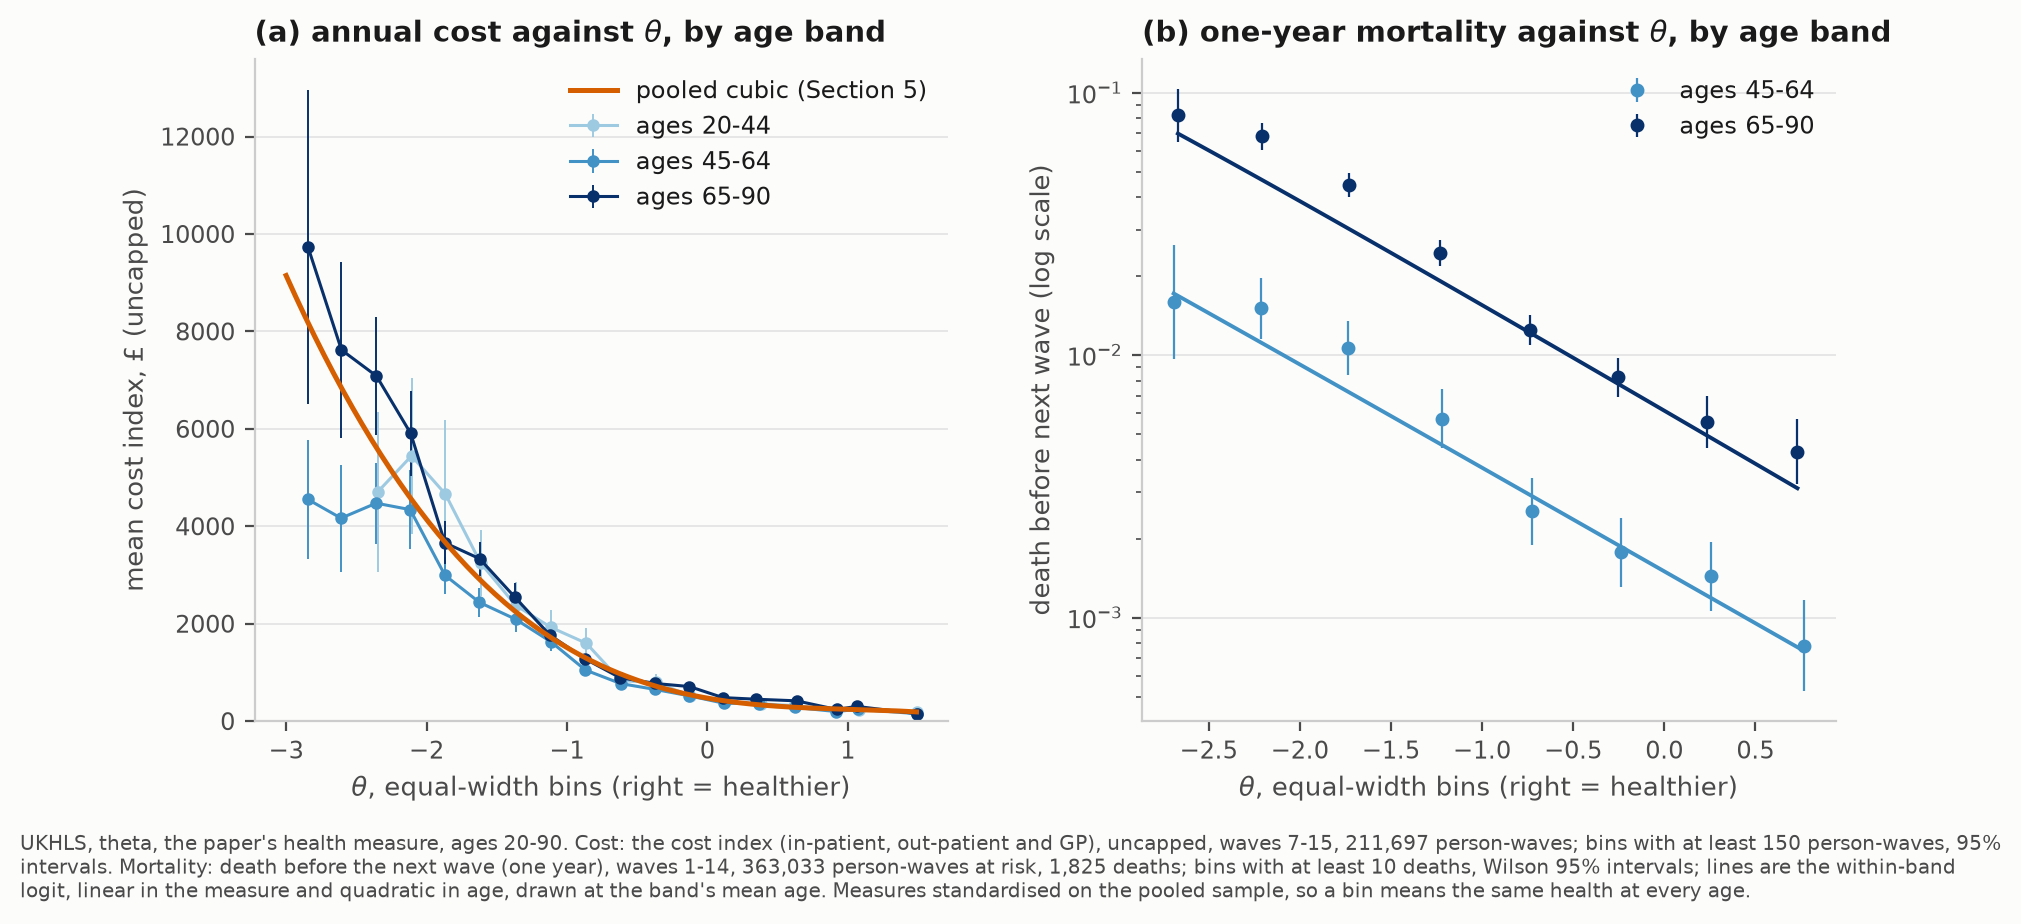
\includegraphics[width=\linewidth]{fig_cost_mortality_age.png}
	\caption{Cost (a) and one-year mortality (b) against $\theta$, by age band; orange line in (a) is the pooled cubic used for pricing.}
	\label{fig:cost}
\end{figure}

\subsection{The moments of health over the life course} \label{subsec:health_moments}

\begin{figure}[H]\centering
	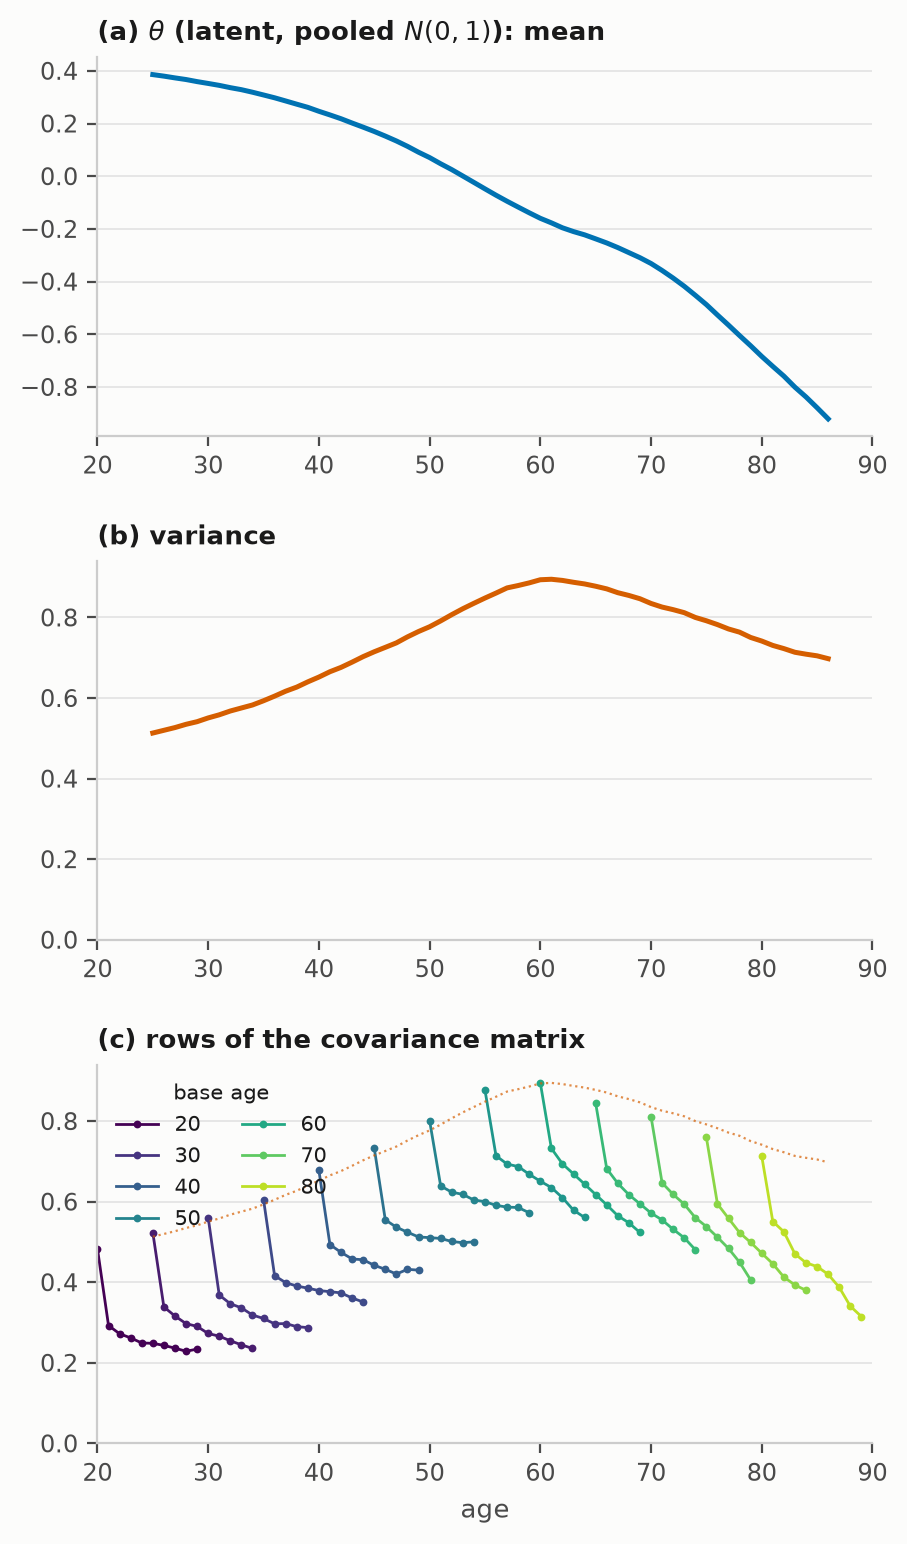
\includegraphics[width=0.55\linewidth]{fig_exhibit1.png}
	\caption{Mean path, variance profile and covariance rows of $\theta$, model-free.}
	\label{fig:exhibit1}
\end{figure}

\begin{itemize}
	\item (a) The mean decline accelerates with age: on its own this says intervene late.
	\item (b) Variance rises 60\% from 30 to 60, peaks at 62, then falls: $C_{Hd}(a)$ turns negative after 60.
	\item (c) A one-year transitory drop in every row, then divergence among the young and convergence among the old.
	\item One stationary noise process cannot produce both, so either noise moves with age or $C_{Hd}$ changes sign. Implication: target the low early; later, targeting on levels pays little.
	\item Same on log frailty; bounded measures ($h$, frailty) keep variance growing after 60.
\end{itemize}

\subsection{The linear approximation on real data} \label{subsec:lin_ident}
\begin{itemize}
	\item Fit $V_H$, $C_{Hd}$, $V_d$ and noise by constrained least squares on the ten moments of four ages four years apart, within four age bands (Case~4: persistent--transitory).
	\item $\Corr(H,d)$ goes from positive to negative with age ($+0.45$, $+0.78$, $-0.56$, $-0.53$); the sign path is robust across cases and measures.
\end{itemize}

\begin{figure}[H]\centering
	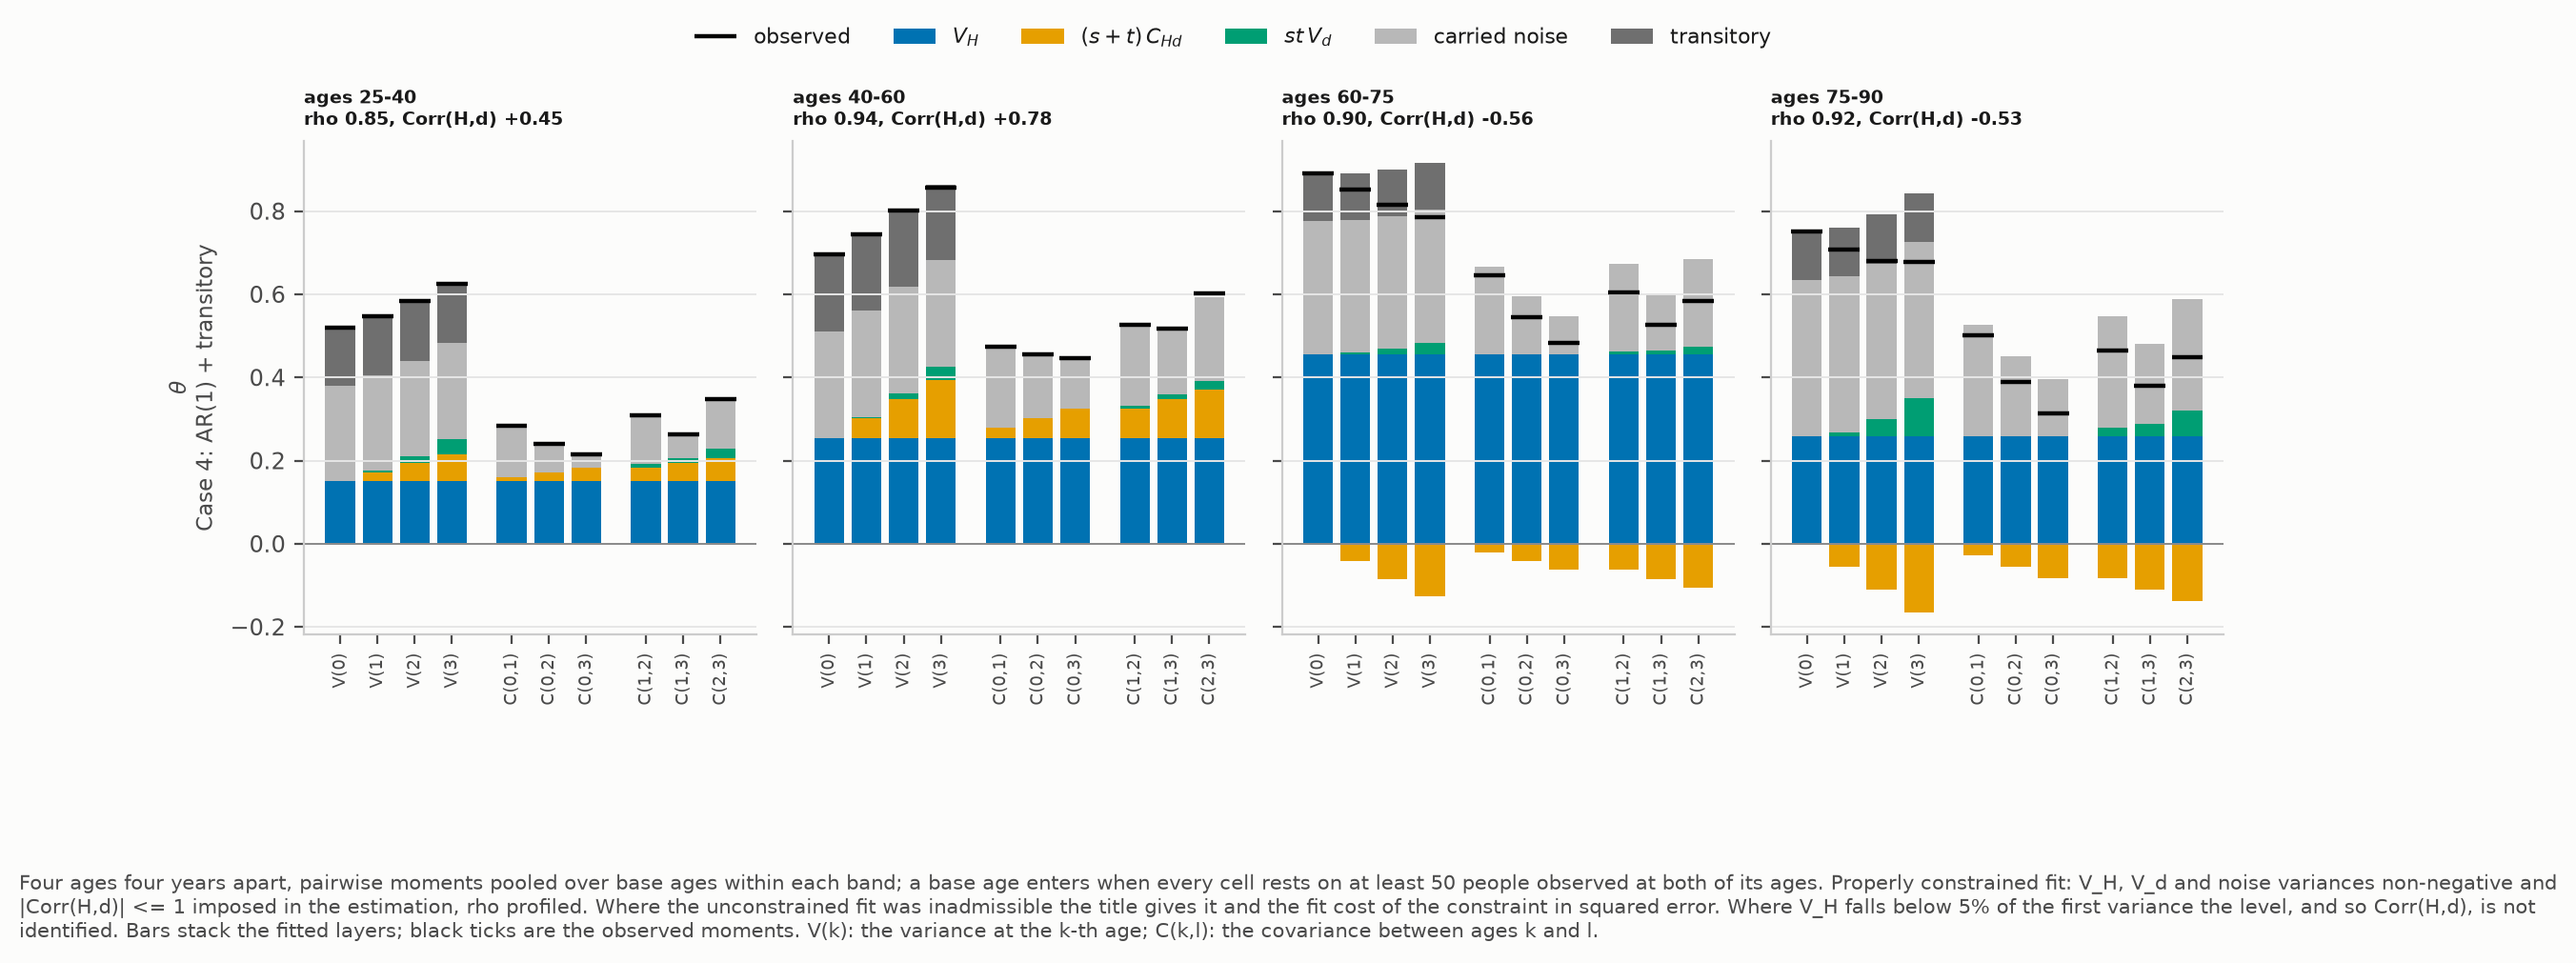
\includegraphics[width=\linewidth]{fig_exhibit2_main.png}
	\caption{The linear approximation on $\theta$, Case~4: fitted layers against observed moments by age band.}
	\label{fig:ex2main}
\end{figure}

\open{which identification cases to present here, and pairwise vs balanced moments; PSID replication to bring in; take posterior uncertainty in $\theta$ into the clustering.}

%% =============================================================================
\section{Lifecycle types}
\label{sec:types}
%% =============================================================================

\subsection{Why and how}
\begin{itemize}
	\item Health at 55 is an outcome of earlier dynamics, and divergence happens before late middle age, so we need the full lifecycle (most work uses the old or short windows).
	\item Cohort-independent types with cohort-dependent shares, estimated three ways: partial K-means, Bayesian mixtures, then against observables.
	\item Challenges: power and type definition; mortality and attrition; cohort effects; units and bounds.
\end{itemize}

\subsection{(A) Non-parametric types: partial K-means}
\begin{itemize}
	\item Minimise squared deviations over observed entries only, $K=3$, 50 starts; every person-wave weighted equally.
	\item Three ordered paths, 18/43/40\%. The worst type falls fastest to 60, then the order reverses: divergence then convergence.
	\item Within-type deviations are persistent (lag-1 autocorrelation 0.37--0.64), so the final model needs persistence.
\end{itemize}

\begin{figure}[H]\centering
	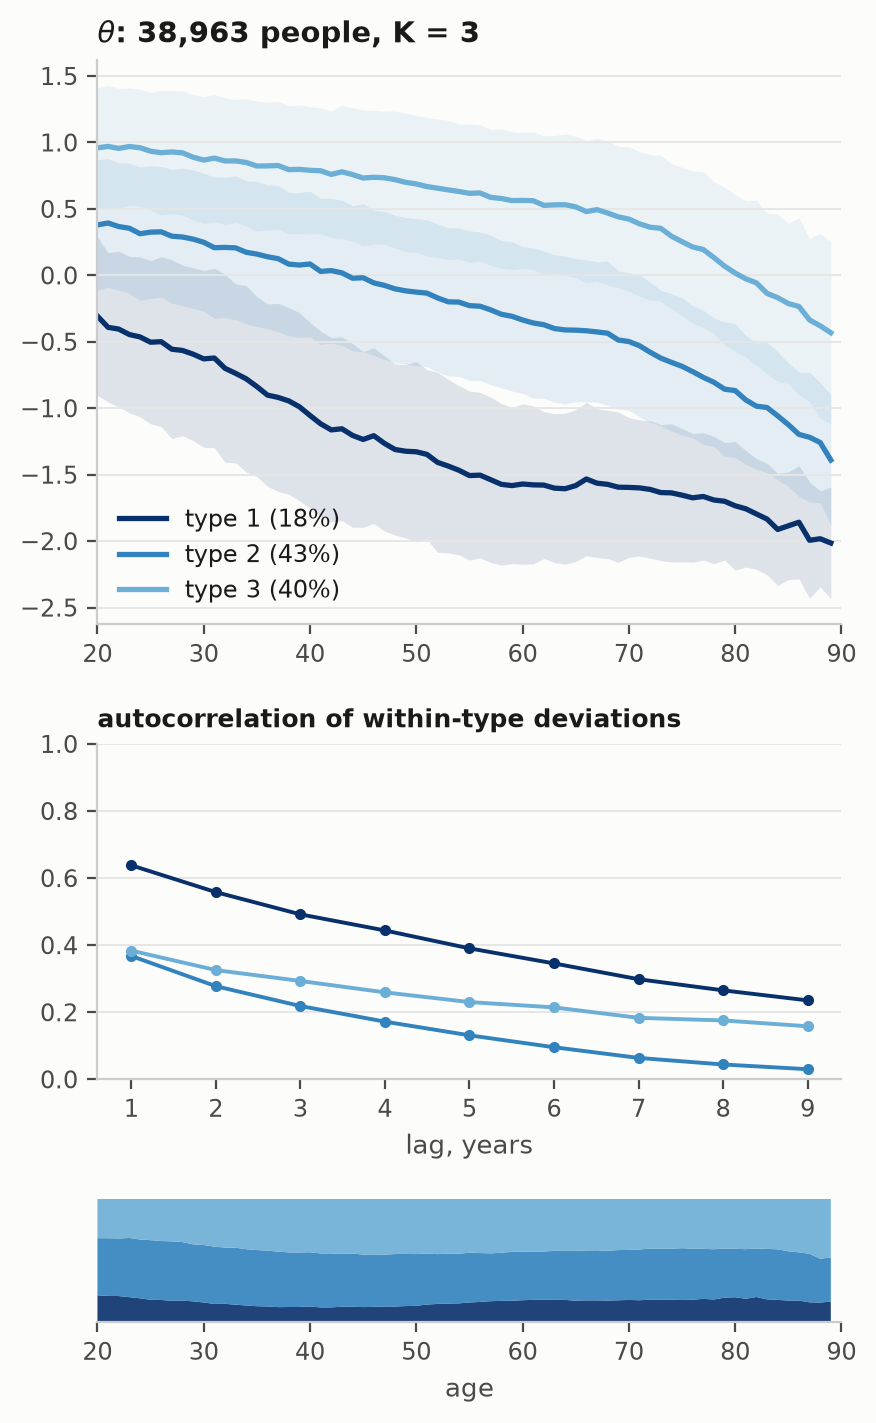
\includegraphics[width=0.55\linewidth]{fig_clusters.png}
	\caption{Partial K-means types ($K=3$) on $\theta$: type means, within-type autocorrelation, composition by age.}
	\label{fig:clusters}
\end{figure}

\begin{itemize}
	\item Between-type share of variance 48\% at 30, 65\% at 70; $\Cov_j(\bar h_{j,a},d_{j,a})$ changes sign at 61.
	\item Cohort adjustment leaves the typology unchanged (ARI 0.90).
\end{itemize}

\begin{figure}[H]\centering
	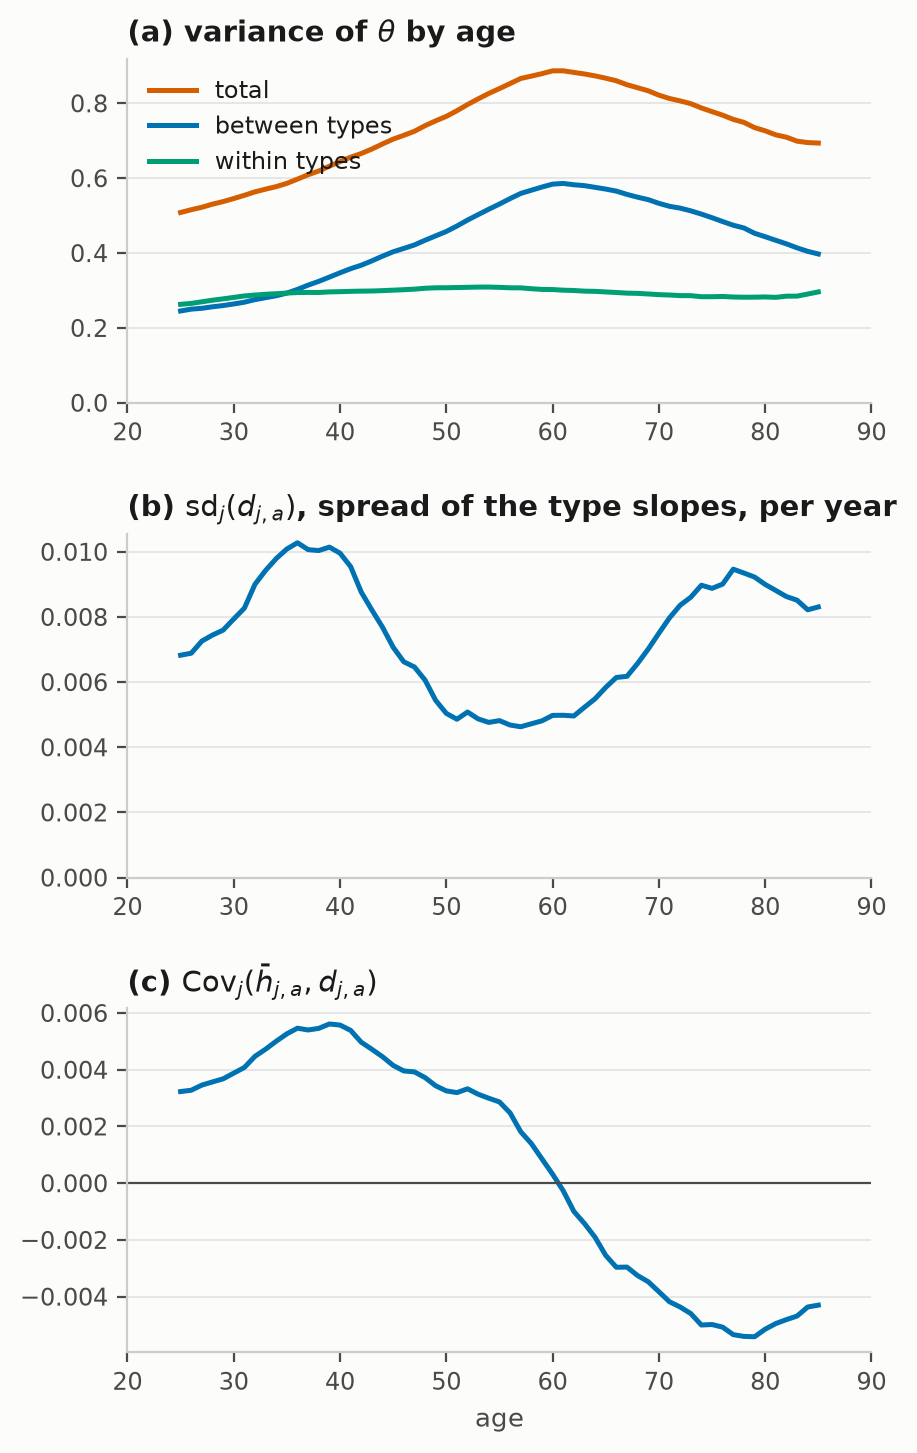
\includegraphics[width=0.55\linewidth]{fig_cluster_decomposition.png}
	\caption{Between versus within by age for the K-means types: variance split, spread of type slopes, level--slope covariance.}
	\label{fig:decomp}
\end{figure}

\subsection{(B) Parametric types: Bayesian mixtures} \label{subsec:parametric}
\begin{itemize}
	\item Baseline: mixture of quadratic growth curves, $\tilde a=(a-55)/10$, estimated in Stan:
	\begin{equation}
		y_{ia}=\alpha_{k_i}+\beta_{k_i}\tilde a+\gamma_{k_i}\tilde a^{2}+\varepsilon_{ia},\qquad \varepsilon_{ia}\sim N(0,\sigma^{2})\ \text{i.i.d.}
		\label{eq:mixbase}
	\end{equation}
	The transitory-only specification; same typology as K-means (ARI 0.85, 95\% same class).
	\item Main specification, persistent--transitory: an AR(1) state plus a transitory shock:
	\begin{equation}
		y_{ia}=\mu_{k_i}(a)+u_{ia}+\varepsilon_{ia},\qquad u_{ia}=\rho_{k_i}^{\,g}\,u_{i,a-g}+\eta_{ia},\quad \eta_{ia}\sim N\Bigl(0,\ \sigma^{2}\tfrac{1-\rho_{k_i}^{2g}}{1-\rho_{k_i}^{2}}\Bigr),\quad \varepsilon_{ia}\sim N(0,\sigma_{\varepsilon}^{2}).
		\label{eq:mixssm}
	\end{equation}
	Shares .25/.47/.29, persistence .87--.96. The worst class now starts near average and falls away.
	\item On $h$ and frailty the healthiest class collapses at the bound: one reason to use $\theta$.
\end{itemize}

\begin{figure}[H]\centering
	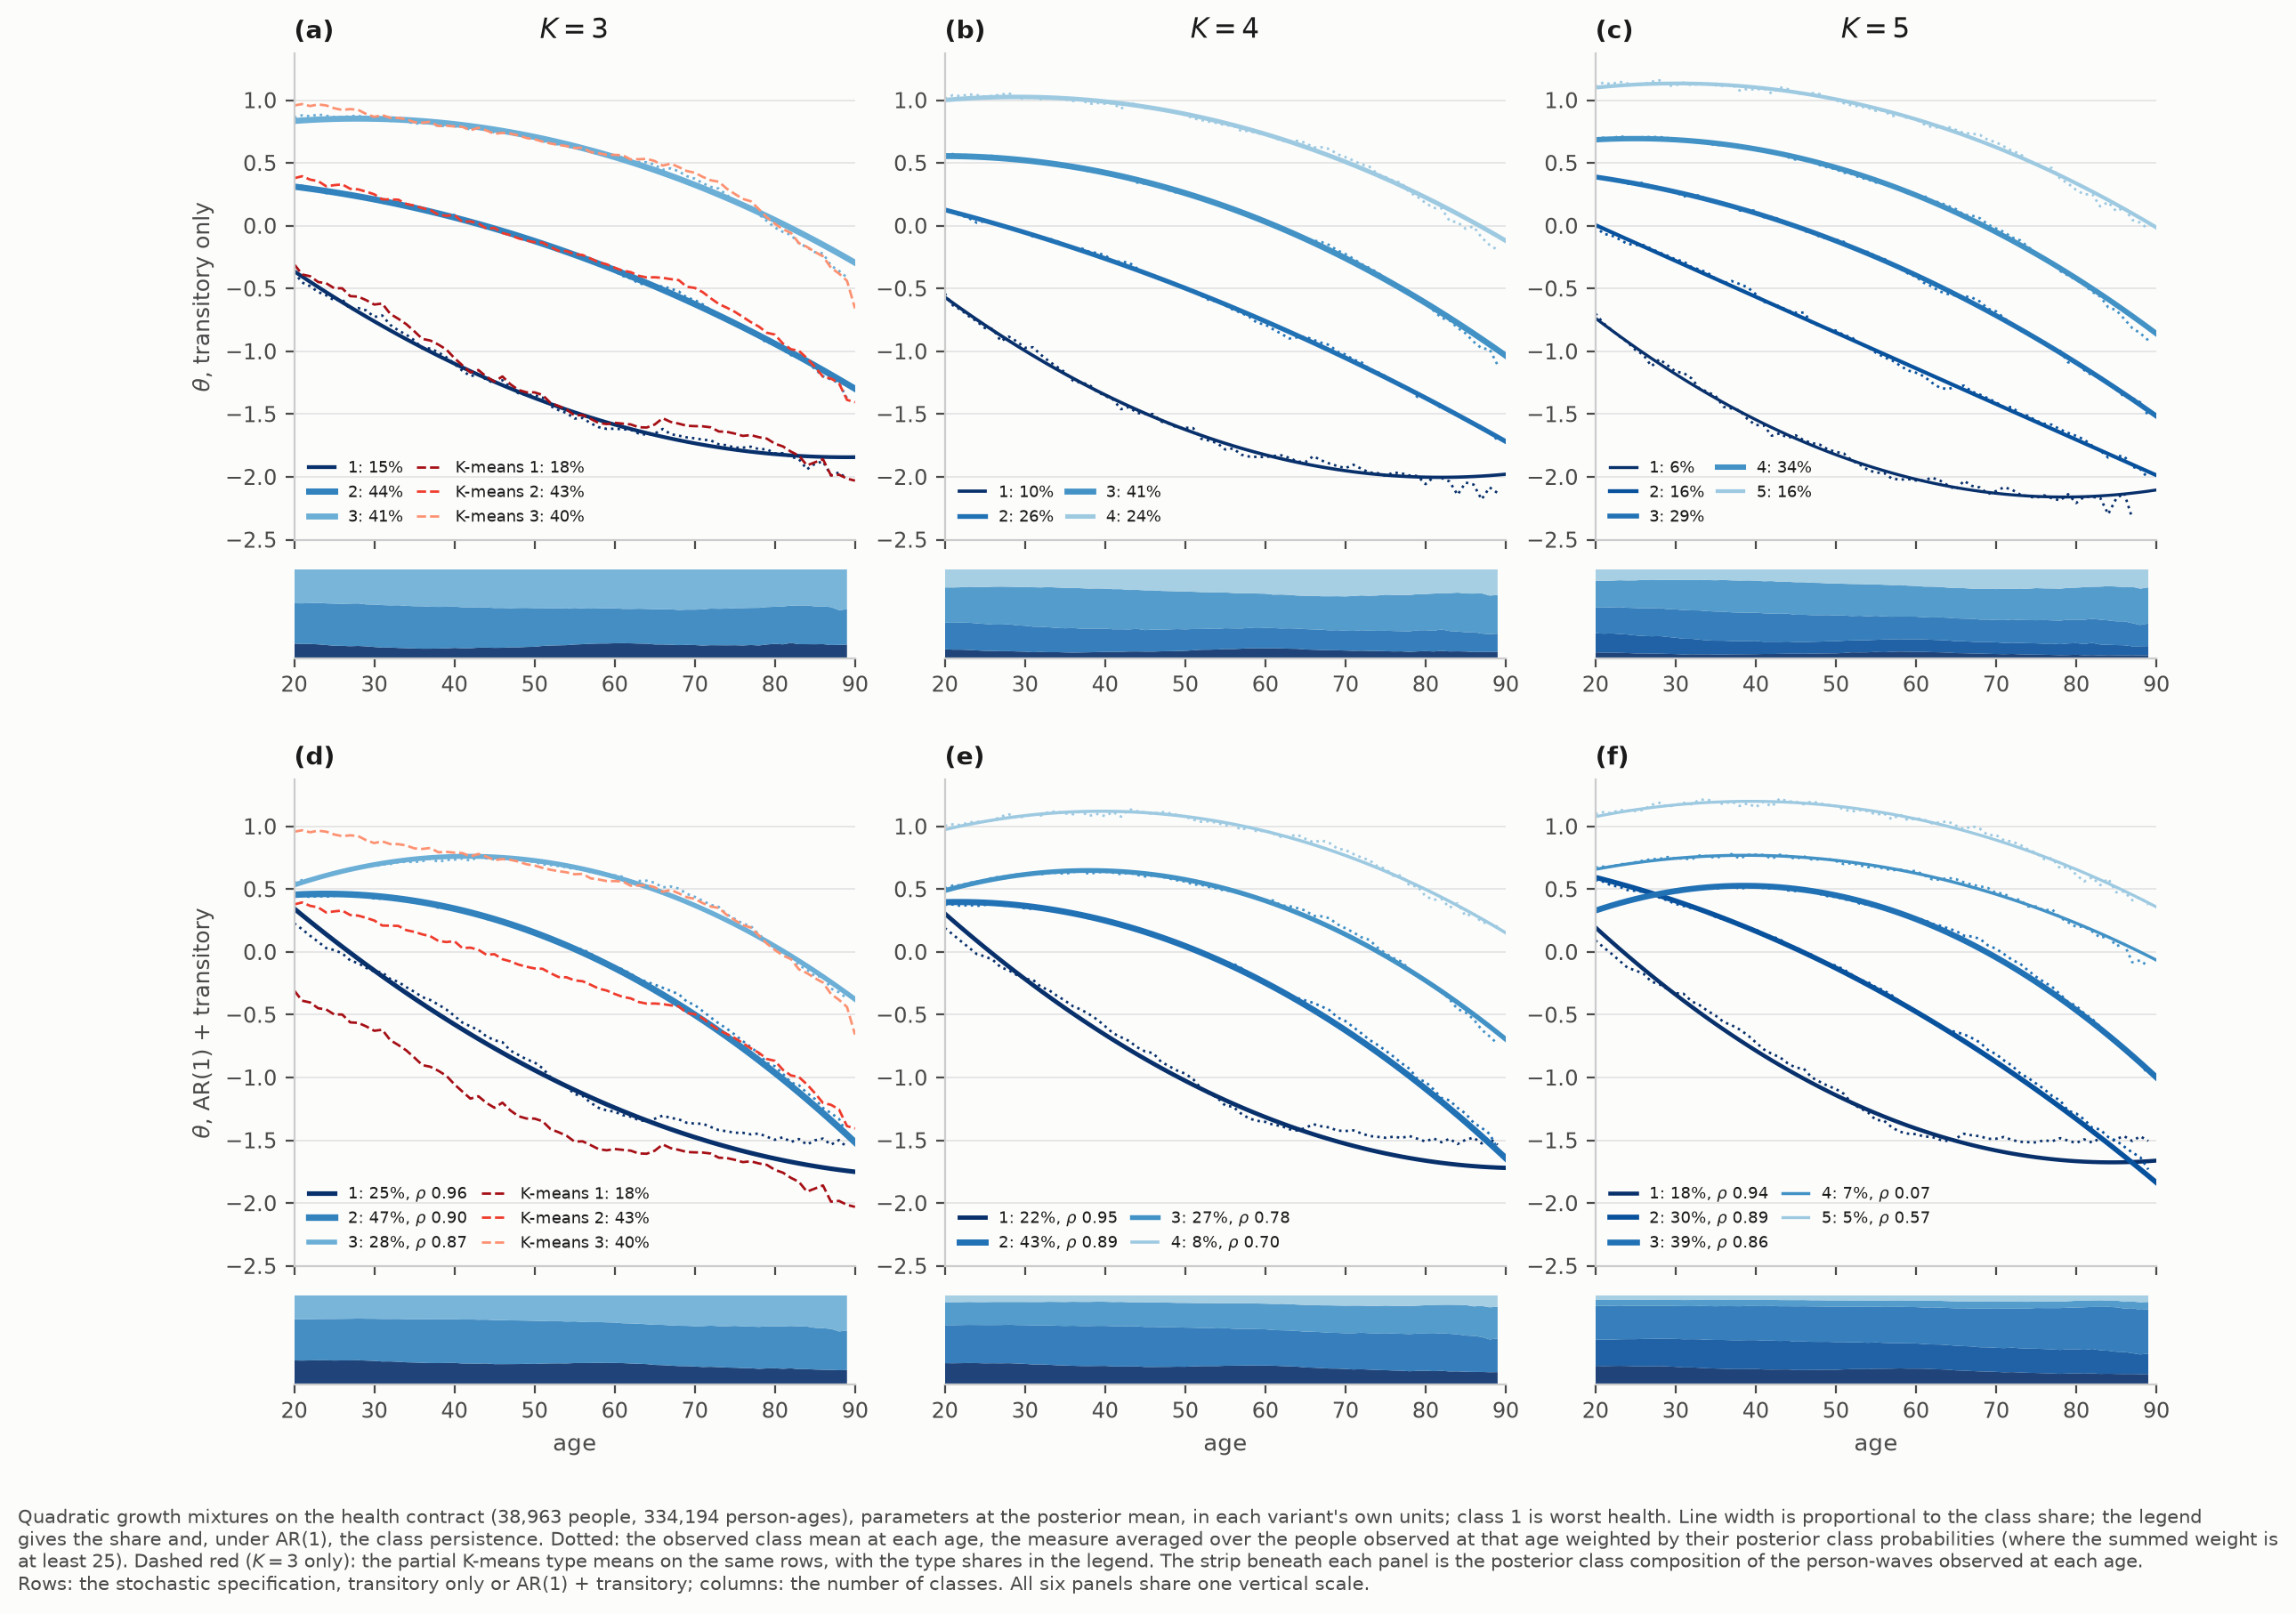
\includegraphics[width=\linewidth]{fig_class_trajectories_by_K.png}
	\caption{Mixtures on $\theta$: transitory only (a)--(c) and persistent--transitory (d)--(f), at $K=3,4,5$; red dashed is K-means.}
	\label{fig:trajK}
\end{figure}

\paragraph{Is there always a bad group?}
\begin{itemize}
	\item Yes, 15--18\% under every method, and mostly the same people (74--85\% overlap).
	\item The stochastic structure changes how they got there: level-based methods overstate early separation and understate decline, and decline is what prevention prices.
	\item This group drives the level--slope reversal: drop it and the reversal disappears.
\end{itemize}

\paragraph{Extensions.}
\begin{itemize}
	\item $K=4,5$: under the transitory-only specification each new class is a sicker group; under the persistent--transitory specification, small healthy groups.
	\item Multidimensional model (physical, mental, Gompertz--Makeham mortality, shared classes): the physical typology survives; mental health is faster and noisier; the worst class's hazard is 11.5$\times$ the best at 55 and 3.2$\times$ at 85.
	\item Windows: a window finds the bad type only if it contains the 40--60 divergence; about fifty years of ages are needed.
	\item Cohort shifts leave the typology unchanged but should not be read as cohort effects (age--cohort collinearity).
	\item Life expectancy from 25: 47.7/57.2/62.2 years; healthy LE separates the classes far more (17.5 vs 59.2).
	\item Death is hard to predict: class adds a little over age (AUC 0.85 to 0.88), less than current health (0.90).
\end{itemize}

\begin{figure}[H]\centering
	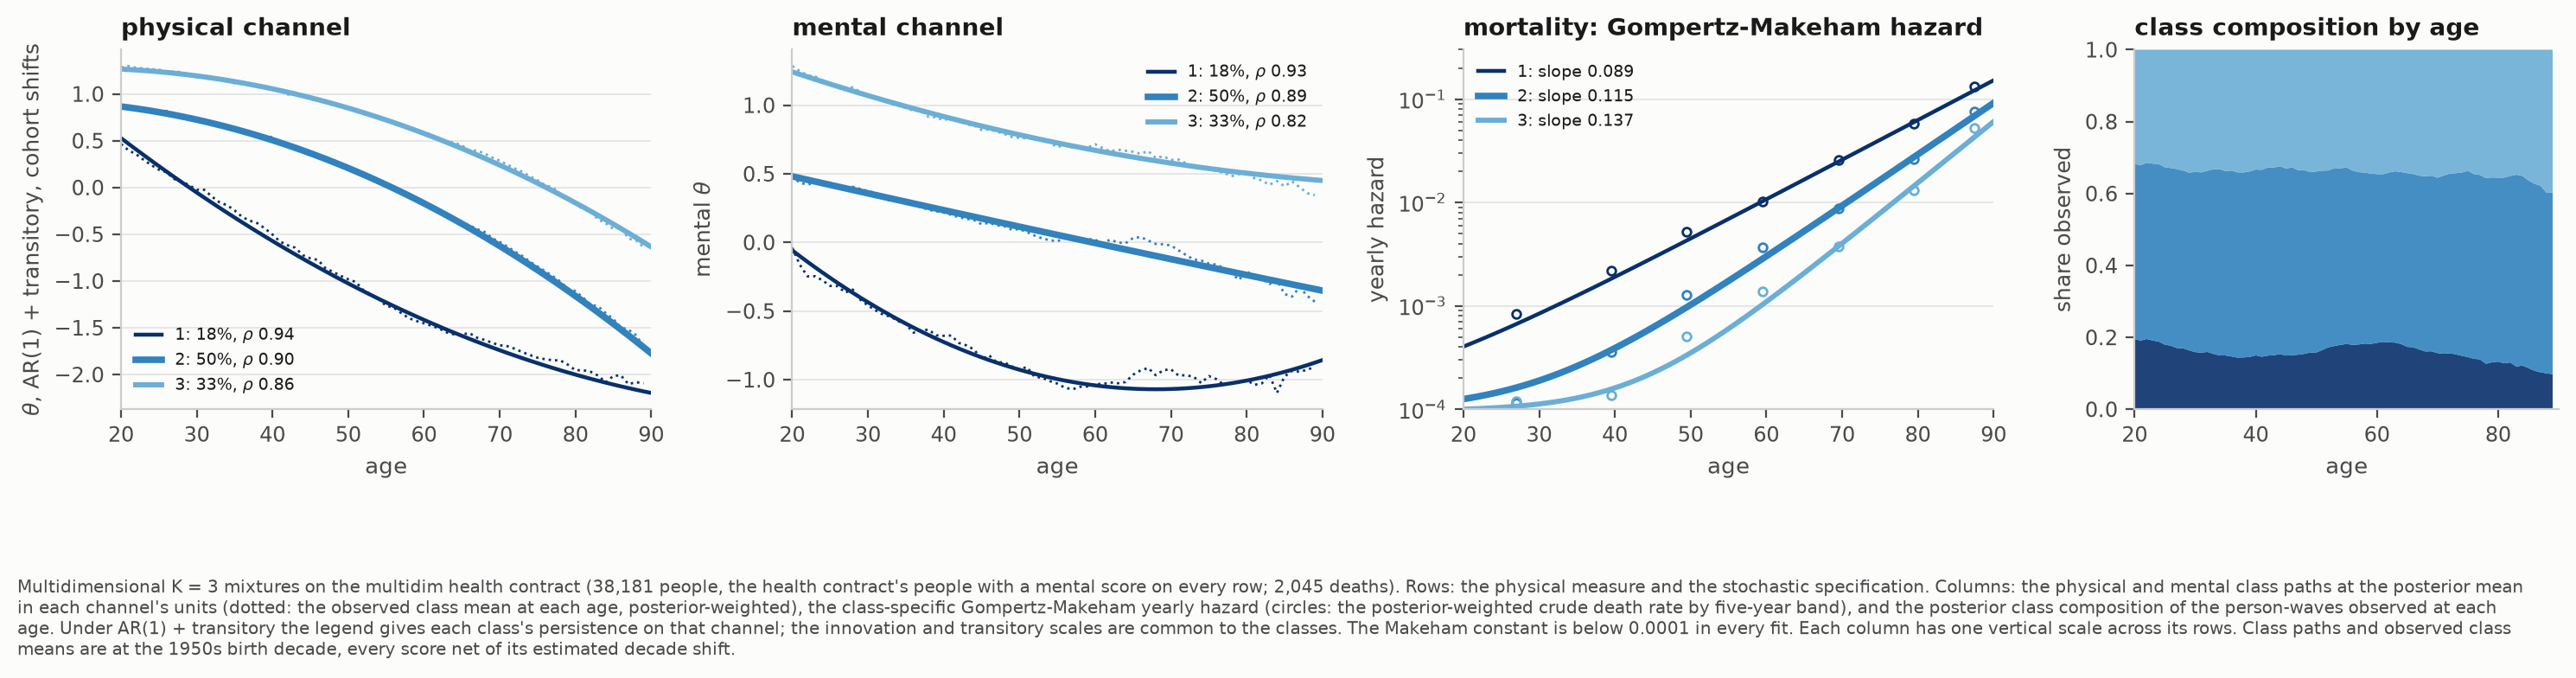
\includegraphics[width=\linewidth]{fig_multidim_trajectories_cohort.png}
	\caption{Multidimensional $K=3$ mixture with birth-decade shifts: physical and mental class paths, class hazards, composition.}
	\label{fig:multidim}
\end{figure}

\begin{figure}[H]\centering
	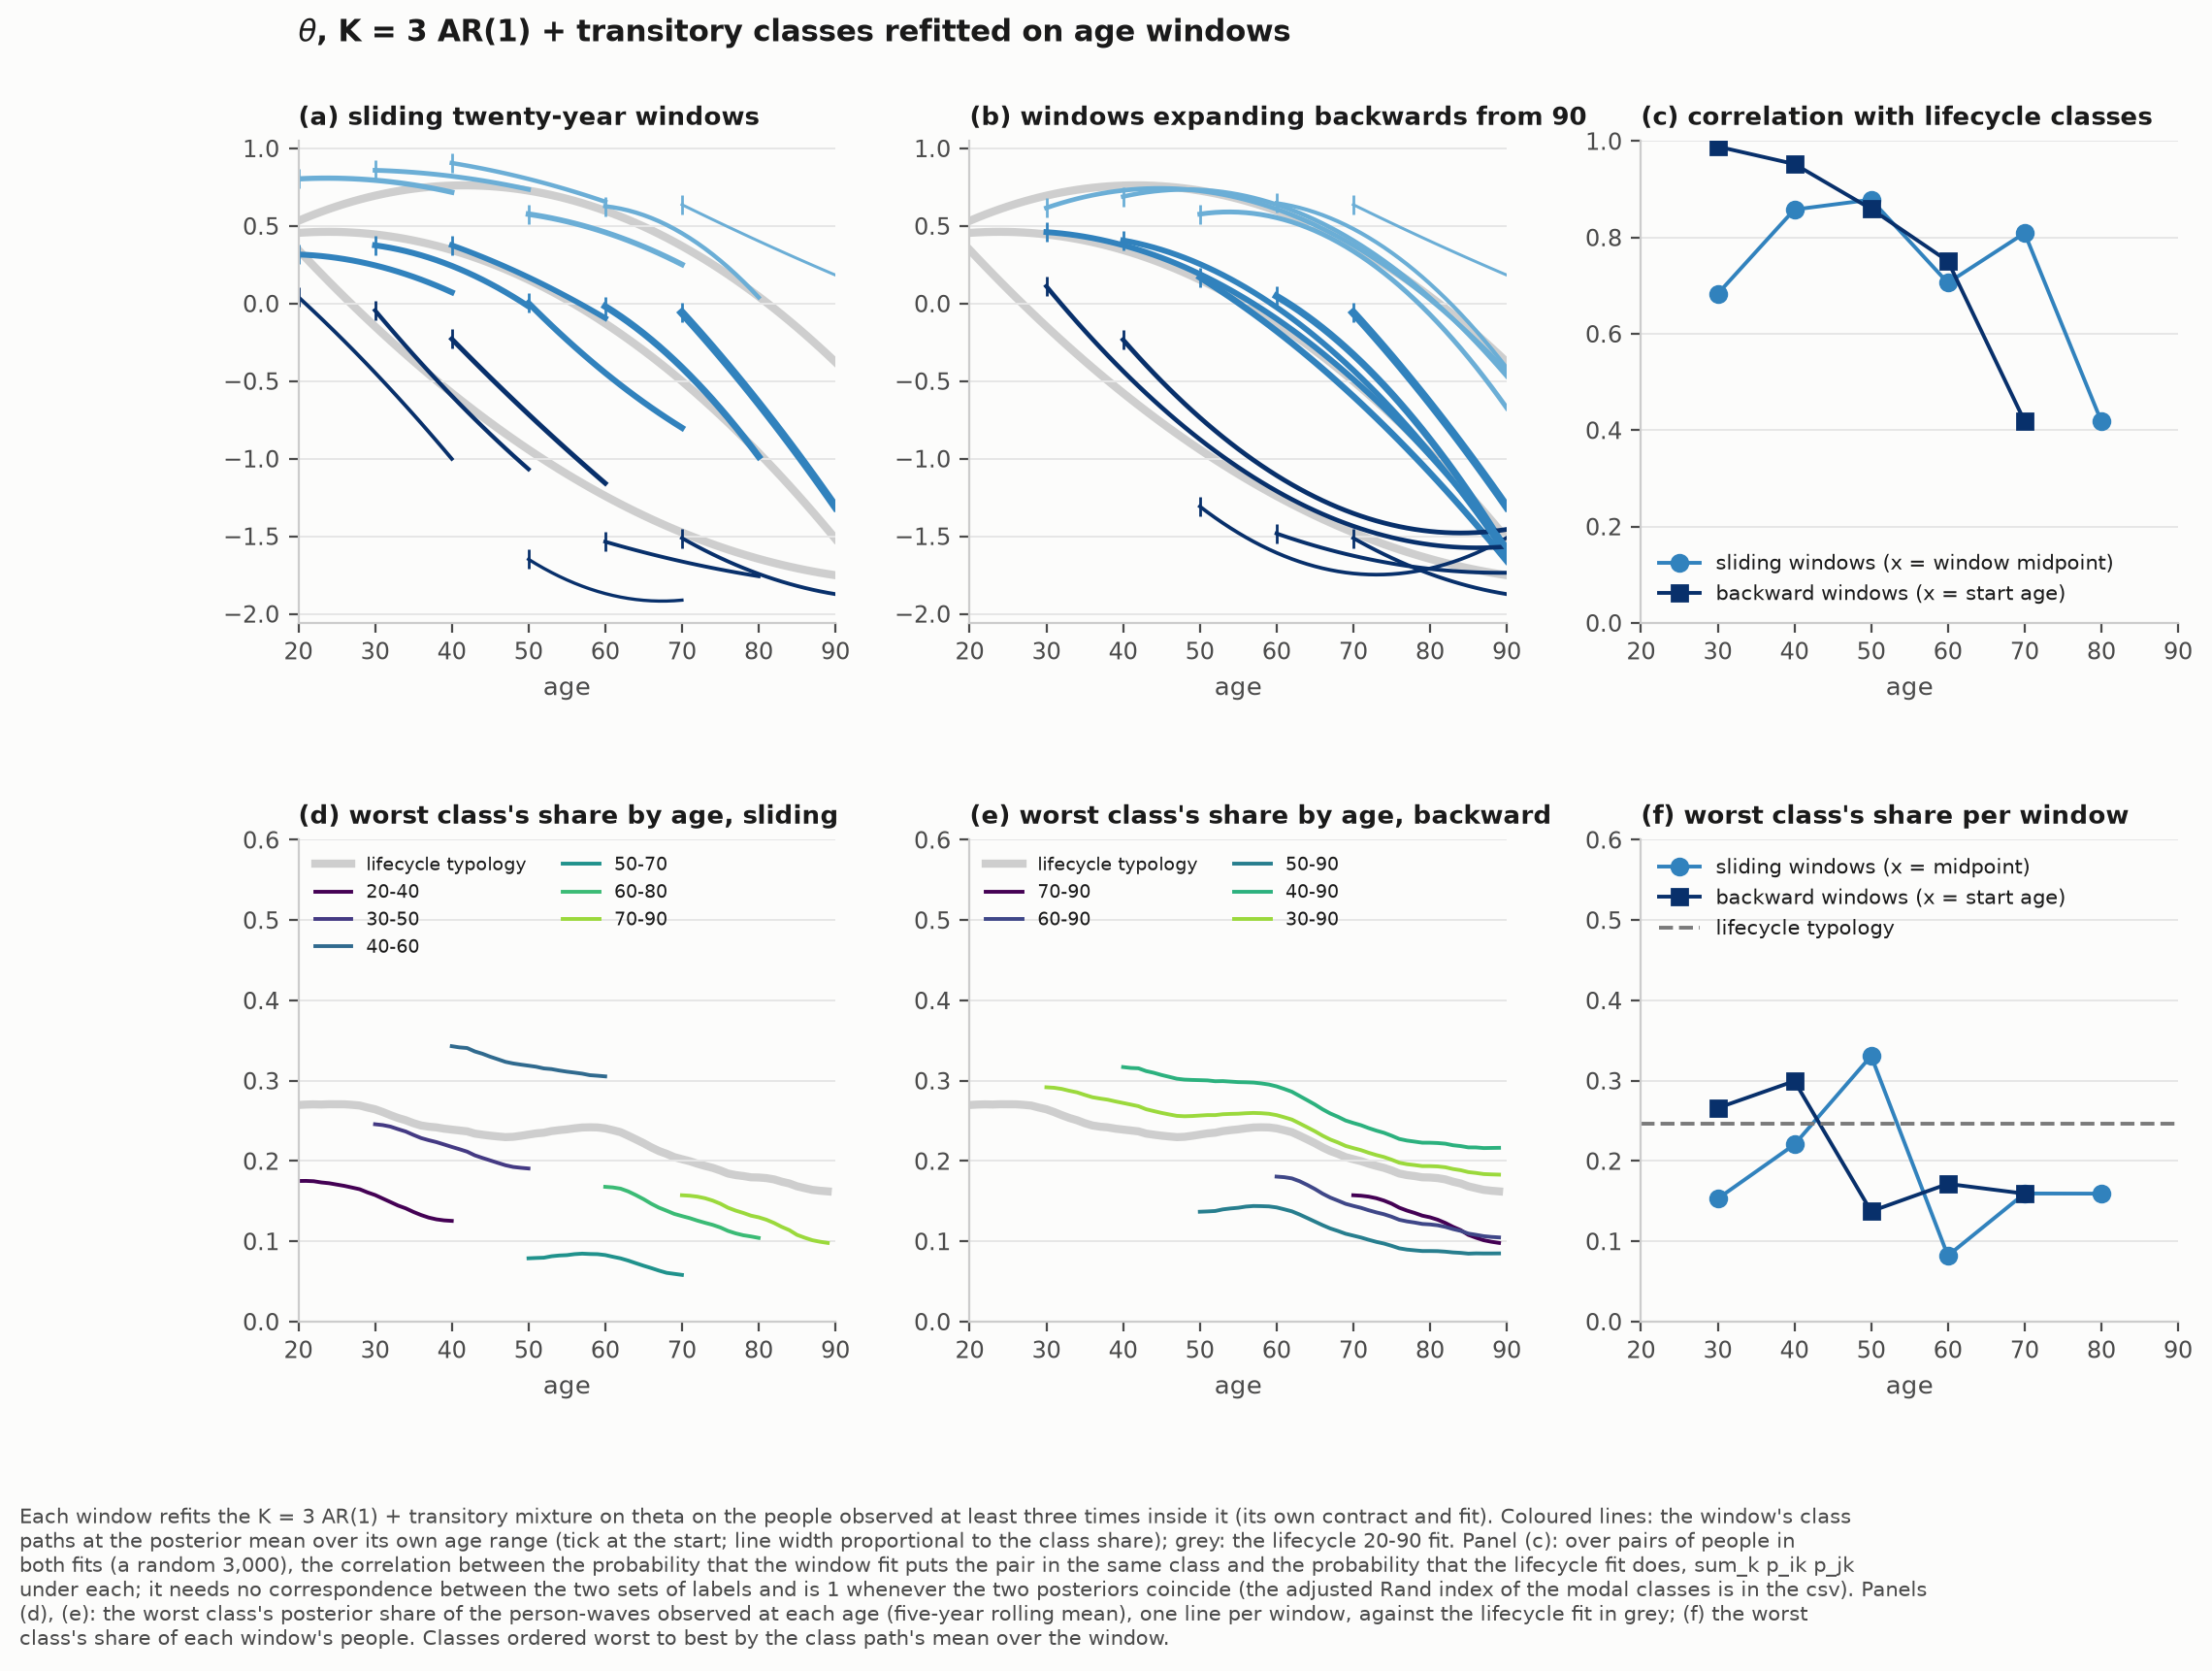
\includegraphics[width=\linewidth]{fig_windows_bayes.png}
	\caption{Persistent--transitory classes refitted on sliding and backward-expanding age windows, agreement with the lifecycle classes, and the worst class's share.}
	\label{fig:windows}
\end{figure}

\subsection{(C) Types against observables}
\label{sec:observables}
\begin{itemize}
	\item Gradients by education and income exist and run the expected way.
	\item But even 40 observable cells span half the range the types do; between-group variance shares 3--9\% against 48--65\% for types; ARI with types 0.01--0.03.
\end{itemize}

\begin{figure}[H]\centering
	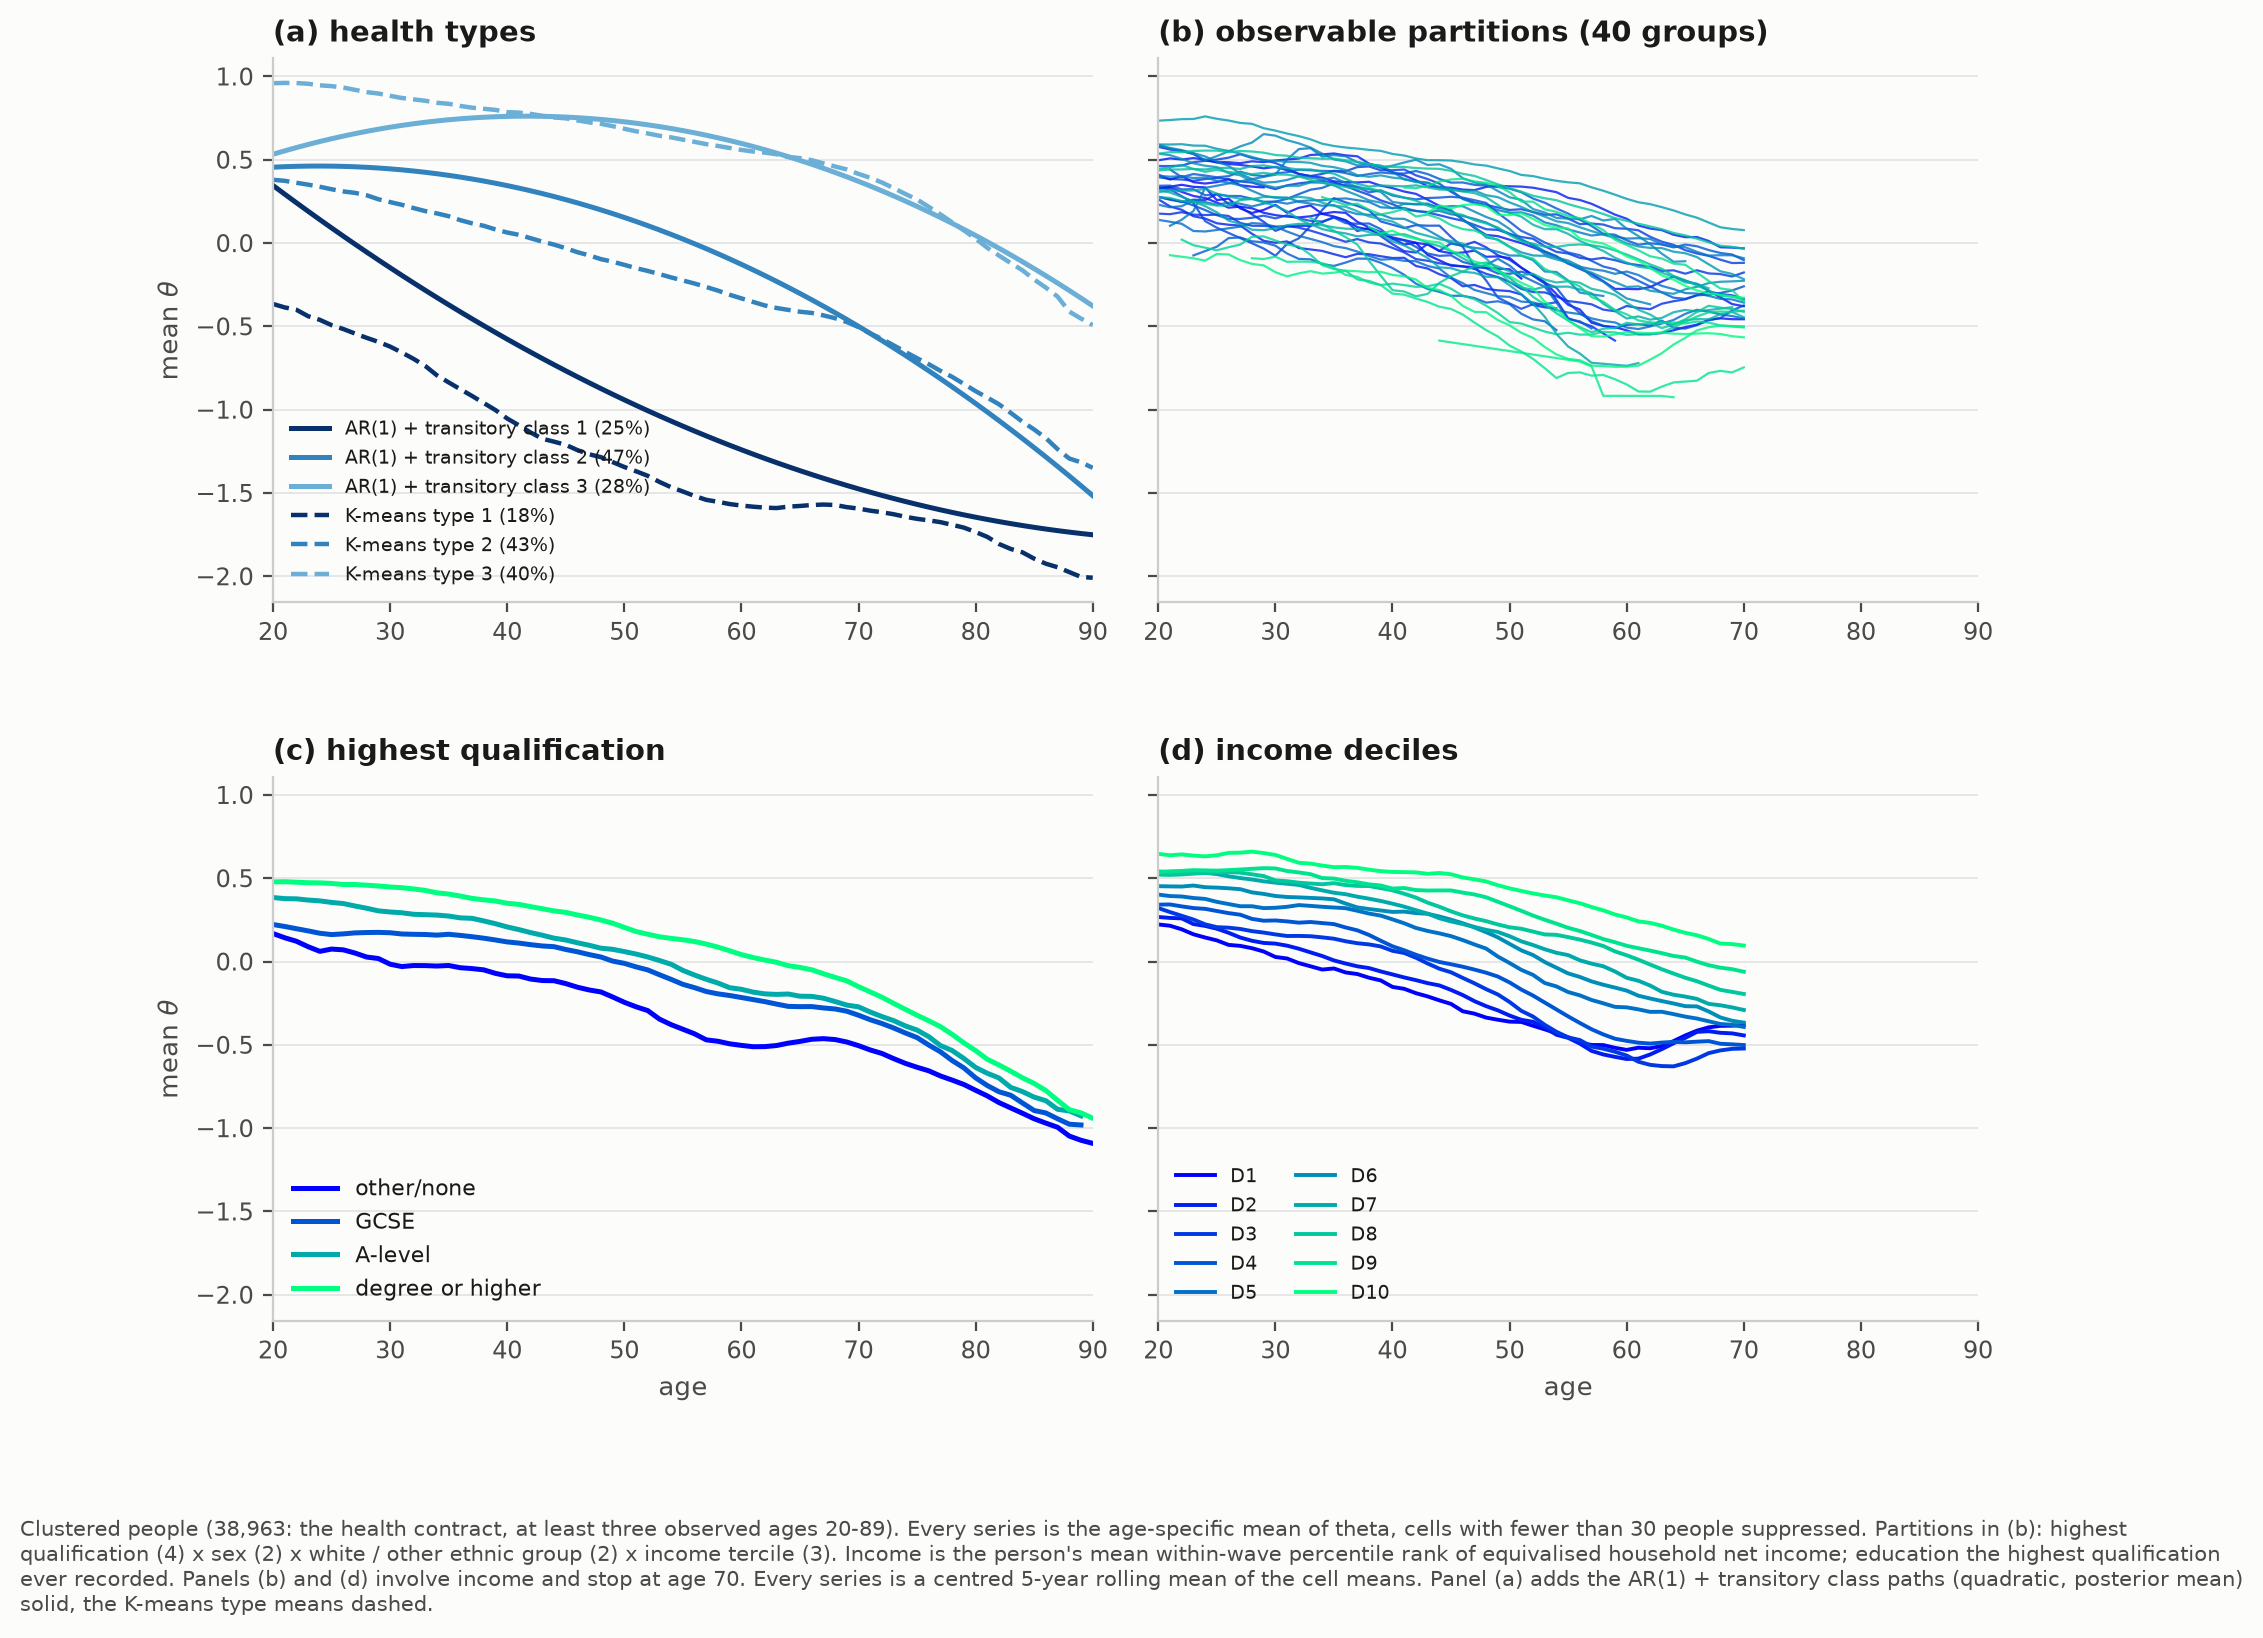
\includegraphics[width=\linewidth]{fig_observables.png}
	\caption{Lifecycle trajectories of $\theta$ by (a) type, (b) 40 observable cells, (c) education, (d) income decile.}
	\label{fig:obs}
\end{figure}

\subsection{Predictive value} \label{subsec:pred}
\begin{itemize}
	\item Predicting ahead (last two rows held out): observables add nothing; current health and the class add about the same; the model forecast does a little better.
	\item Predicting type (first two rows held out): observables barely predict it; one health reading is most of the value; health is the weakest guide to type when young.
	\item Headline: health is what matters, the model helps a bit, observables are almost irrelevant.
\end{itemize}

\begin{figure}[H]\centering
	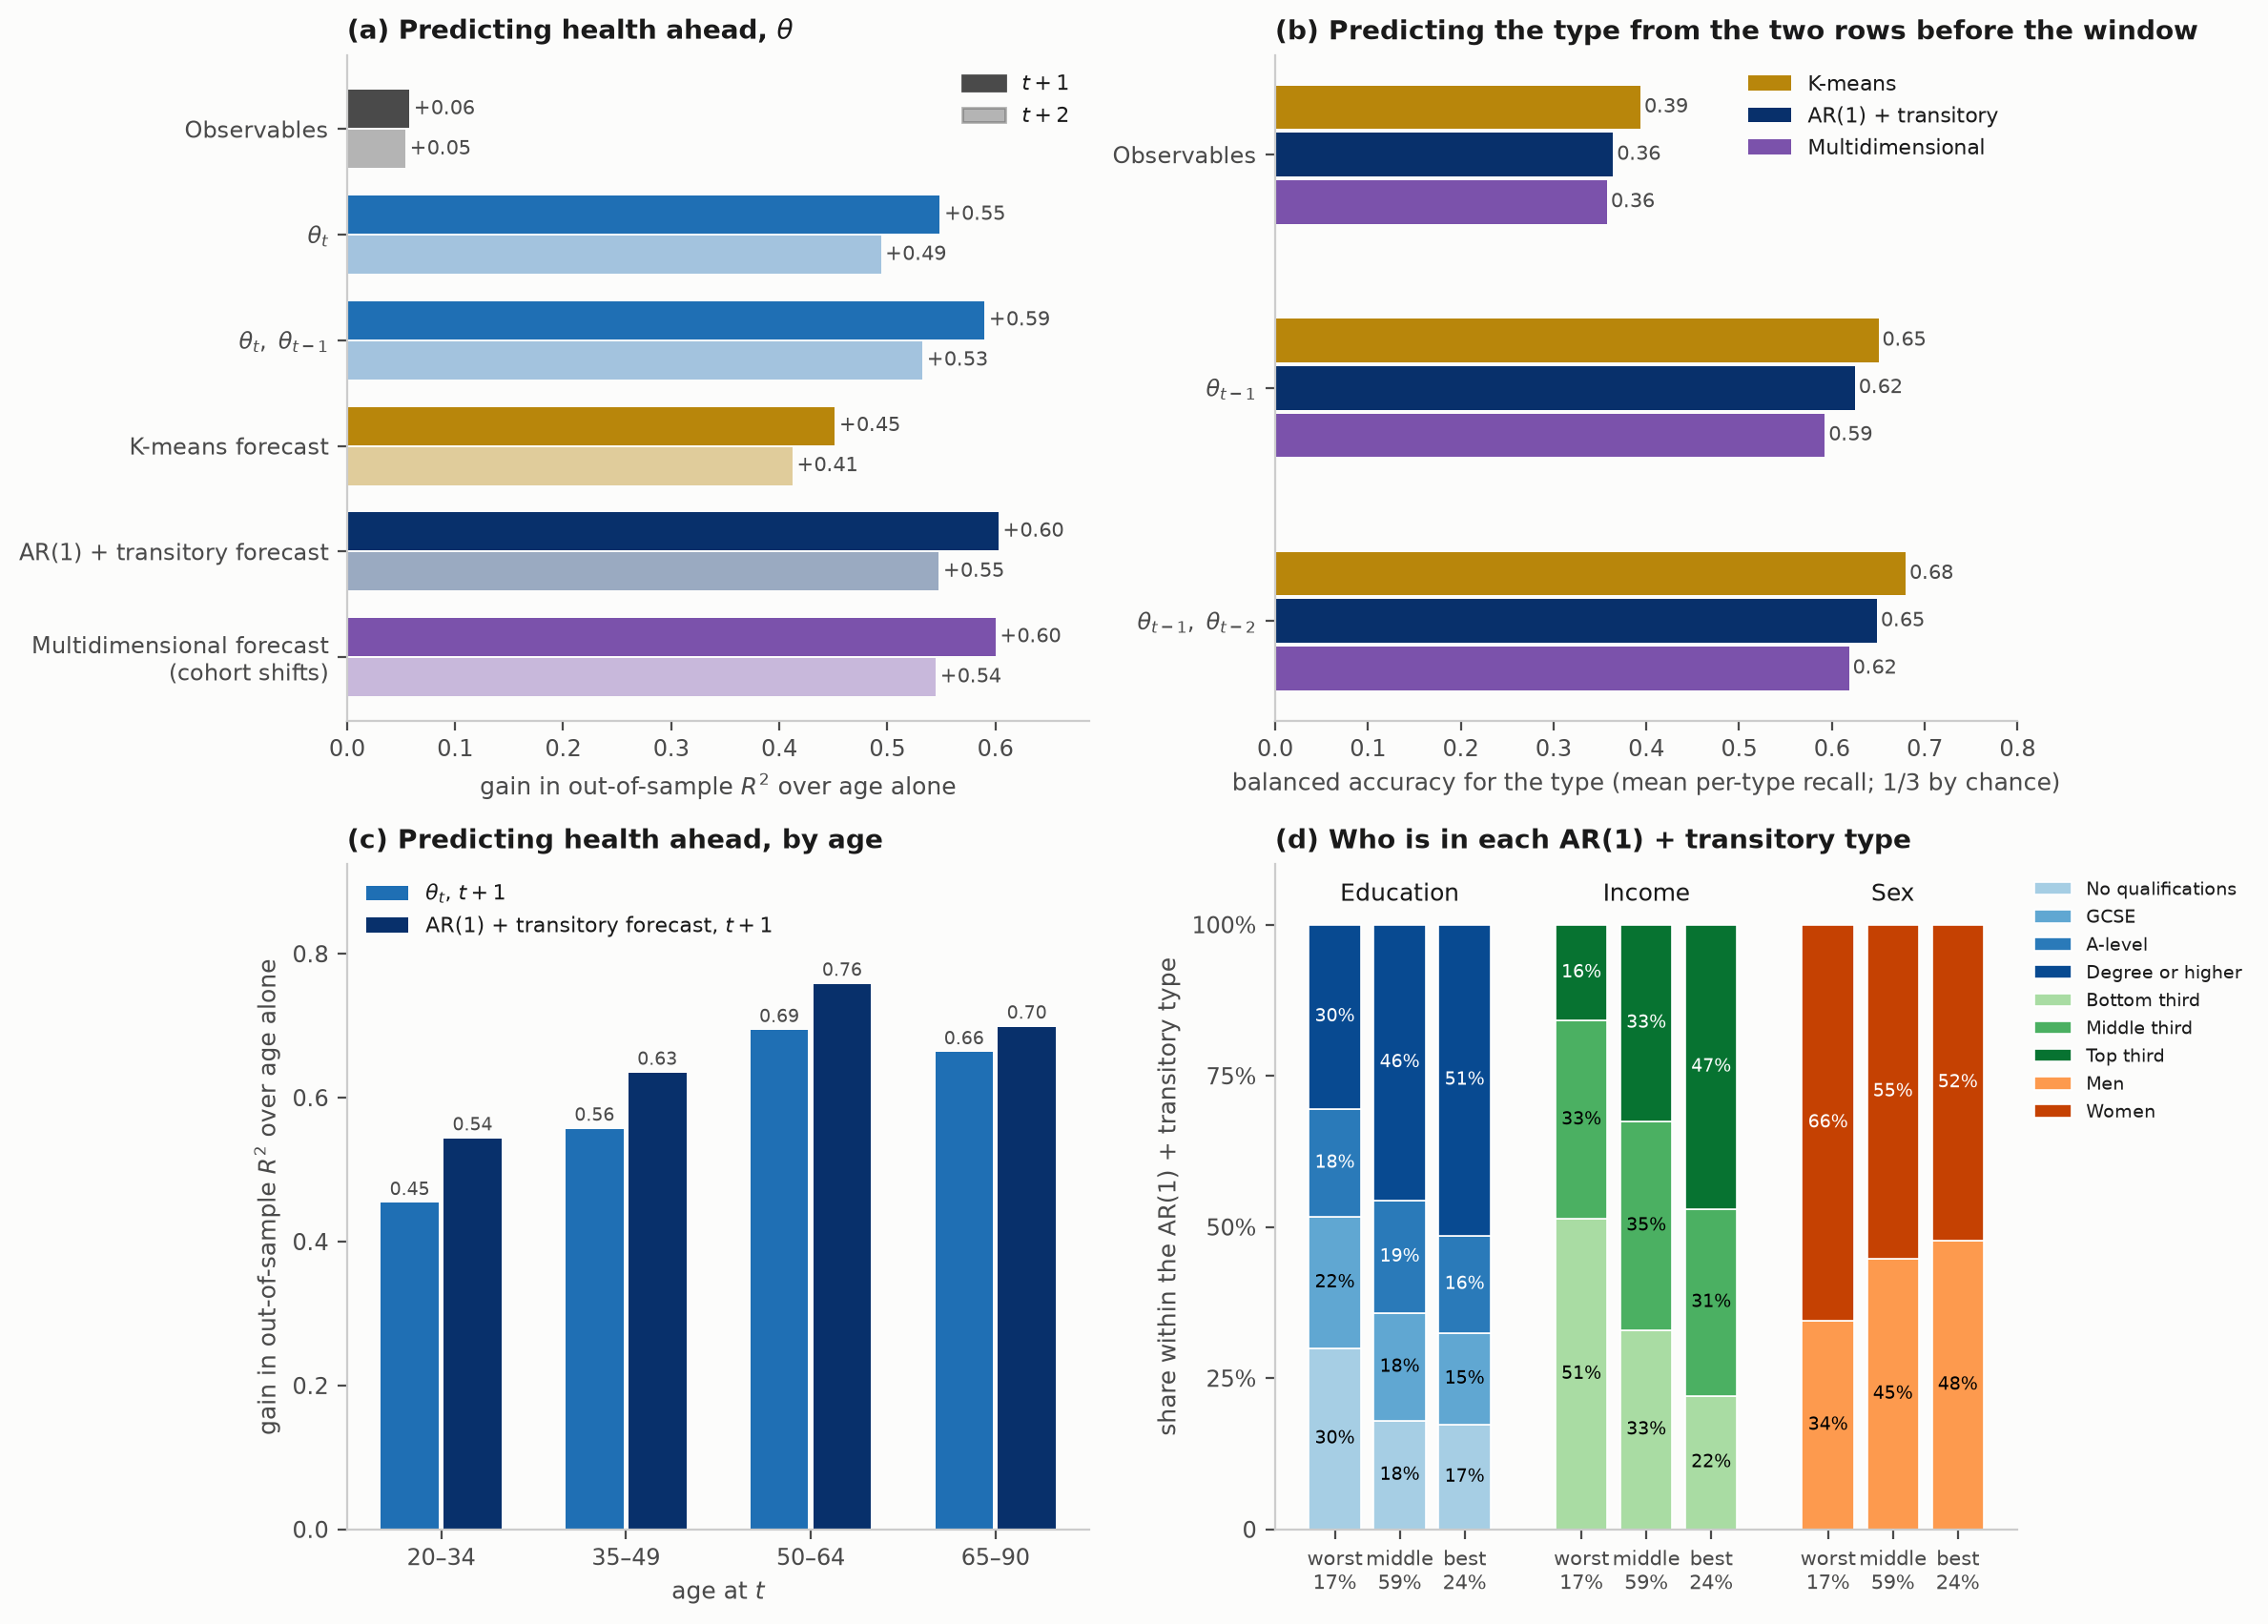
\includegraphics[width=\linewidth]{fig_prediction_summary.png}
	\caption{Out-of-sample gain over age in predicting $\theta$ ahead (a, c) and balanced accuracy in predicting the type (b), with the type composition by observables (d).}
	\label{fig:predsummary}
\end{figure}

\open{bounded observation model for $h$ and frailty; class composition in the persistent--transitory fits looks like mortality selection; calibrate healthy LE to ONS.}

%% =============================================================================
\section{Prevention exercises}
\label{sec:policy}
%% =============================================================================
\begin{itemize}
	\item Priced on the $K=3$ persistent--transitory classes with the estimated cubic cost curve; pounds to 90, undiscounted.
	\item \textbf{The bill}: \pounds67{,}500 per person from 25; 63\% mean path, 16\% type differences, 21\% unpreventable deviations.
	\item \textbf{Uniform prevention}: $P(r)/C(r)$ is 1.17 at 25, 0.78 at 50, 0.45 at 70; the exact saving at $\mu=1$ is 65\%, 52\%, 35\% of the bill. The later the start, the more is already determined.
	\item \textbf{By class}: the worst class returns 2.3$\times$ the uniform amount from 25 because its gap and decline coincide; the best class a tenth.
	\item \textbf{Timing}: the between-class channel stays positive at every start age once the transitory shock is separated (it turns negative by 50 under the transitory-only specification).
	\item \textbf{Targeting on class}: gains of 133\% from 25, 38\% from 50, 51\% from 70.
\end{itemize}

\begin{figure}[H]\centering
	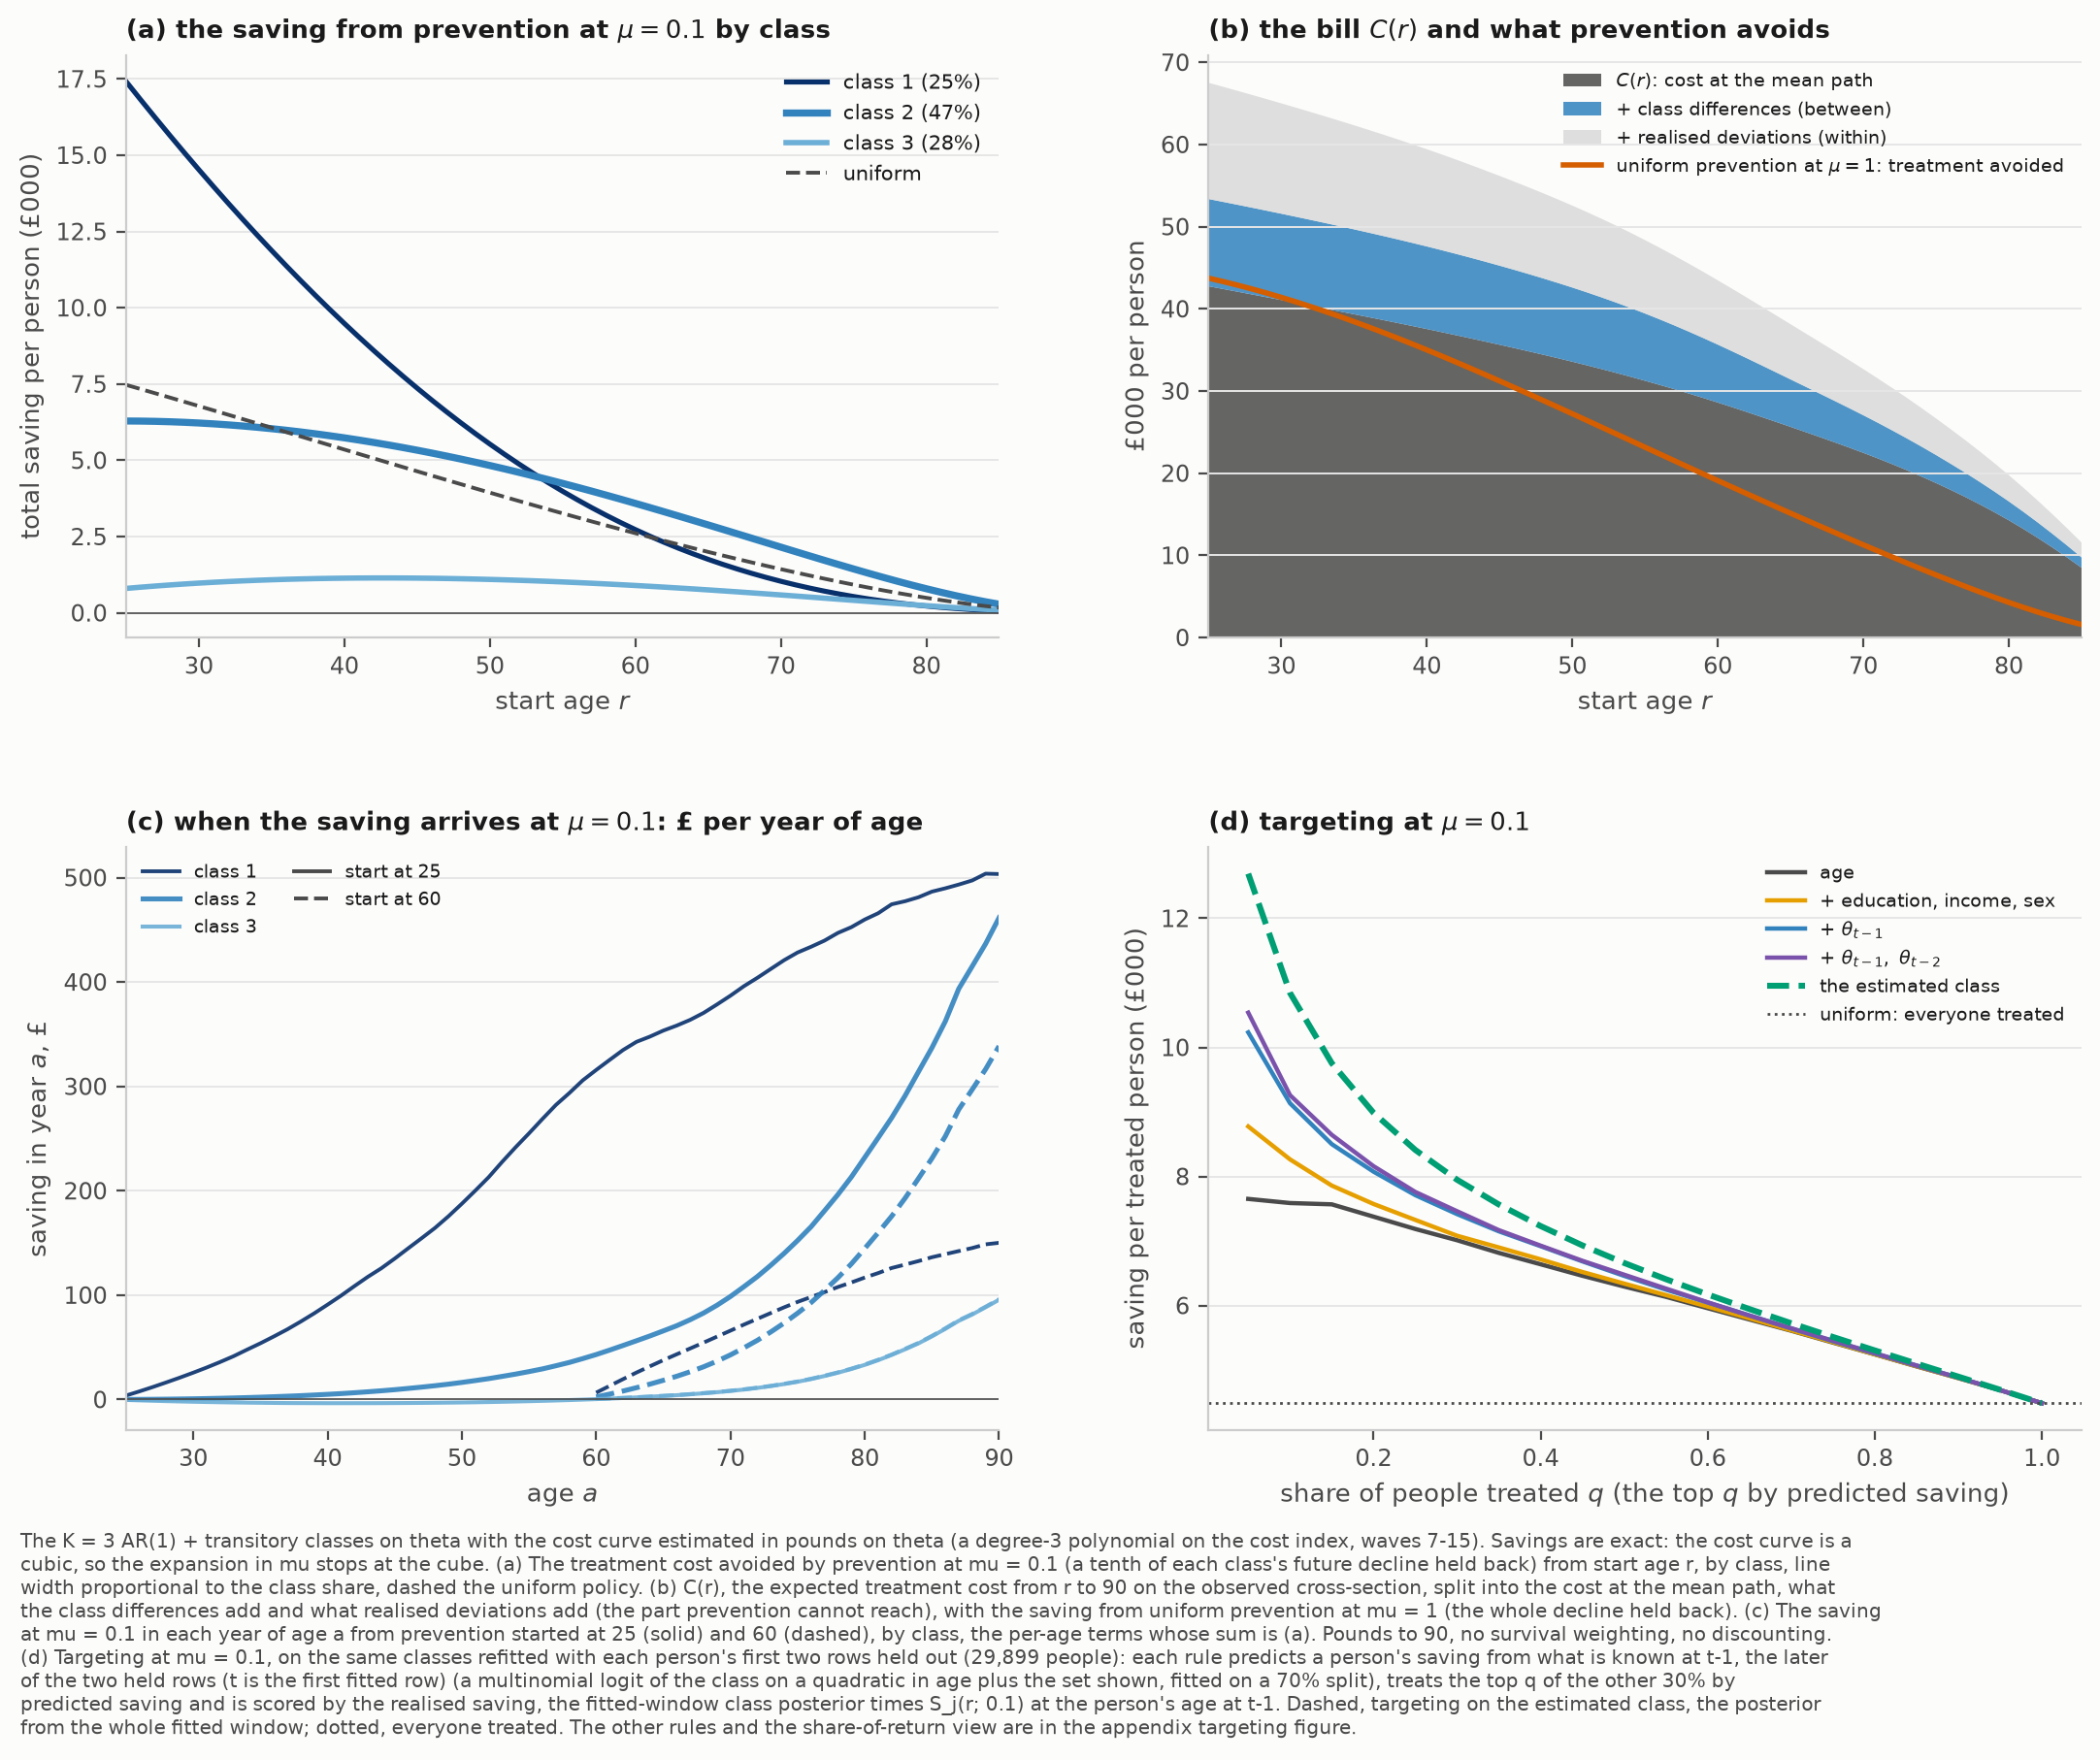
\includegraphics[width=\linewidth]{fig_prevention.png}
	\caption{Prevention in pounds: (a) saving at $\mu=0.1$ by class and start age; (b) the bill $C(r)$ and the uniform saving at $\mu=1$; (c) when the saving arrives; (d) targeting with what is known before the fitted window.}
	\label{fig:prevention}
\end{figure}

\begin{itemize}
	\item \textbf{When}: savings are back-loaded (half by 72 for the worst class, 82 middle, 86 best), so discounting will bite.
	\item \textbf{What to target on}: age first; then a health reading (\pounds9{,}100 per treated person at 10\% coverage) beats observables (\pounds8{,}300); the estimated class gets \pounds10{,}800. Two readings close about half the gap from age to class.
\end{itemize}

\begin{figure}[H]\centering
	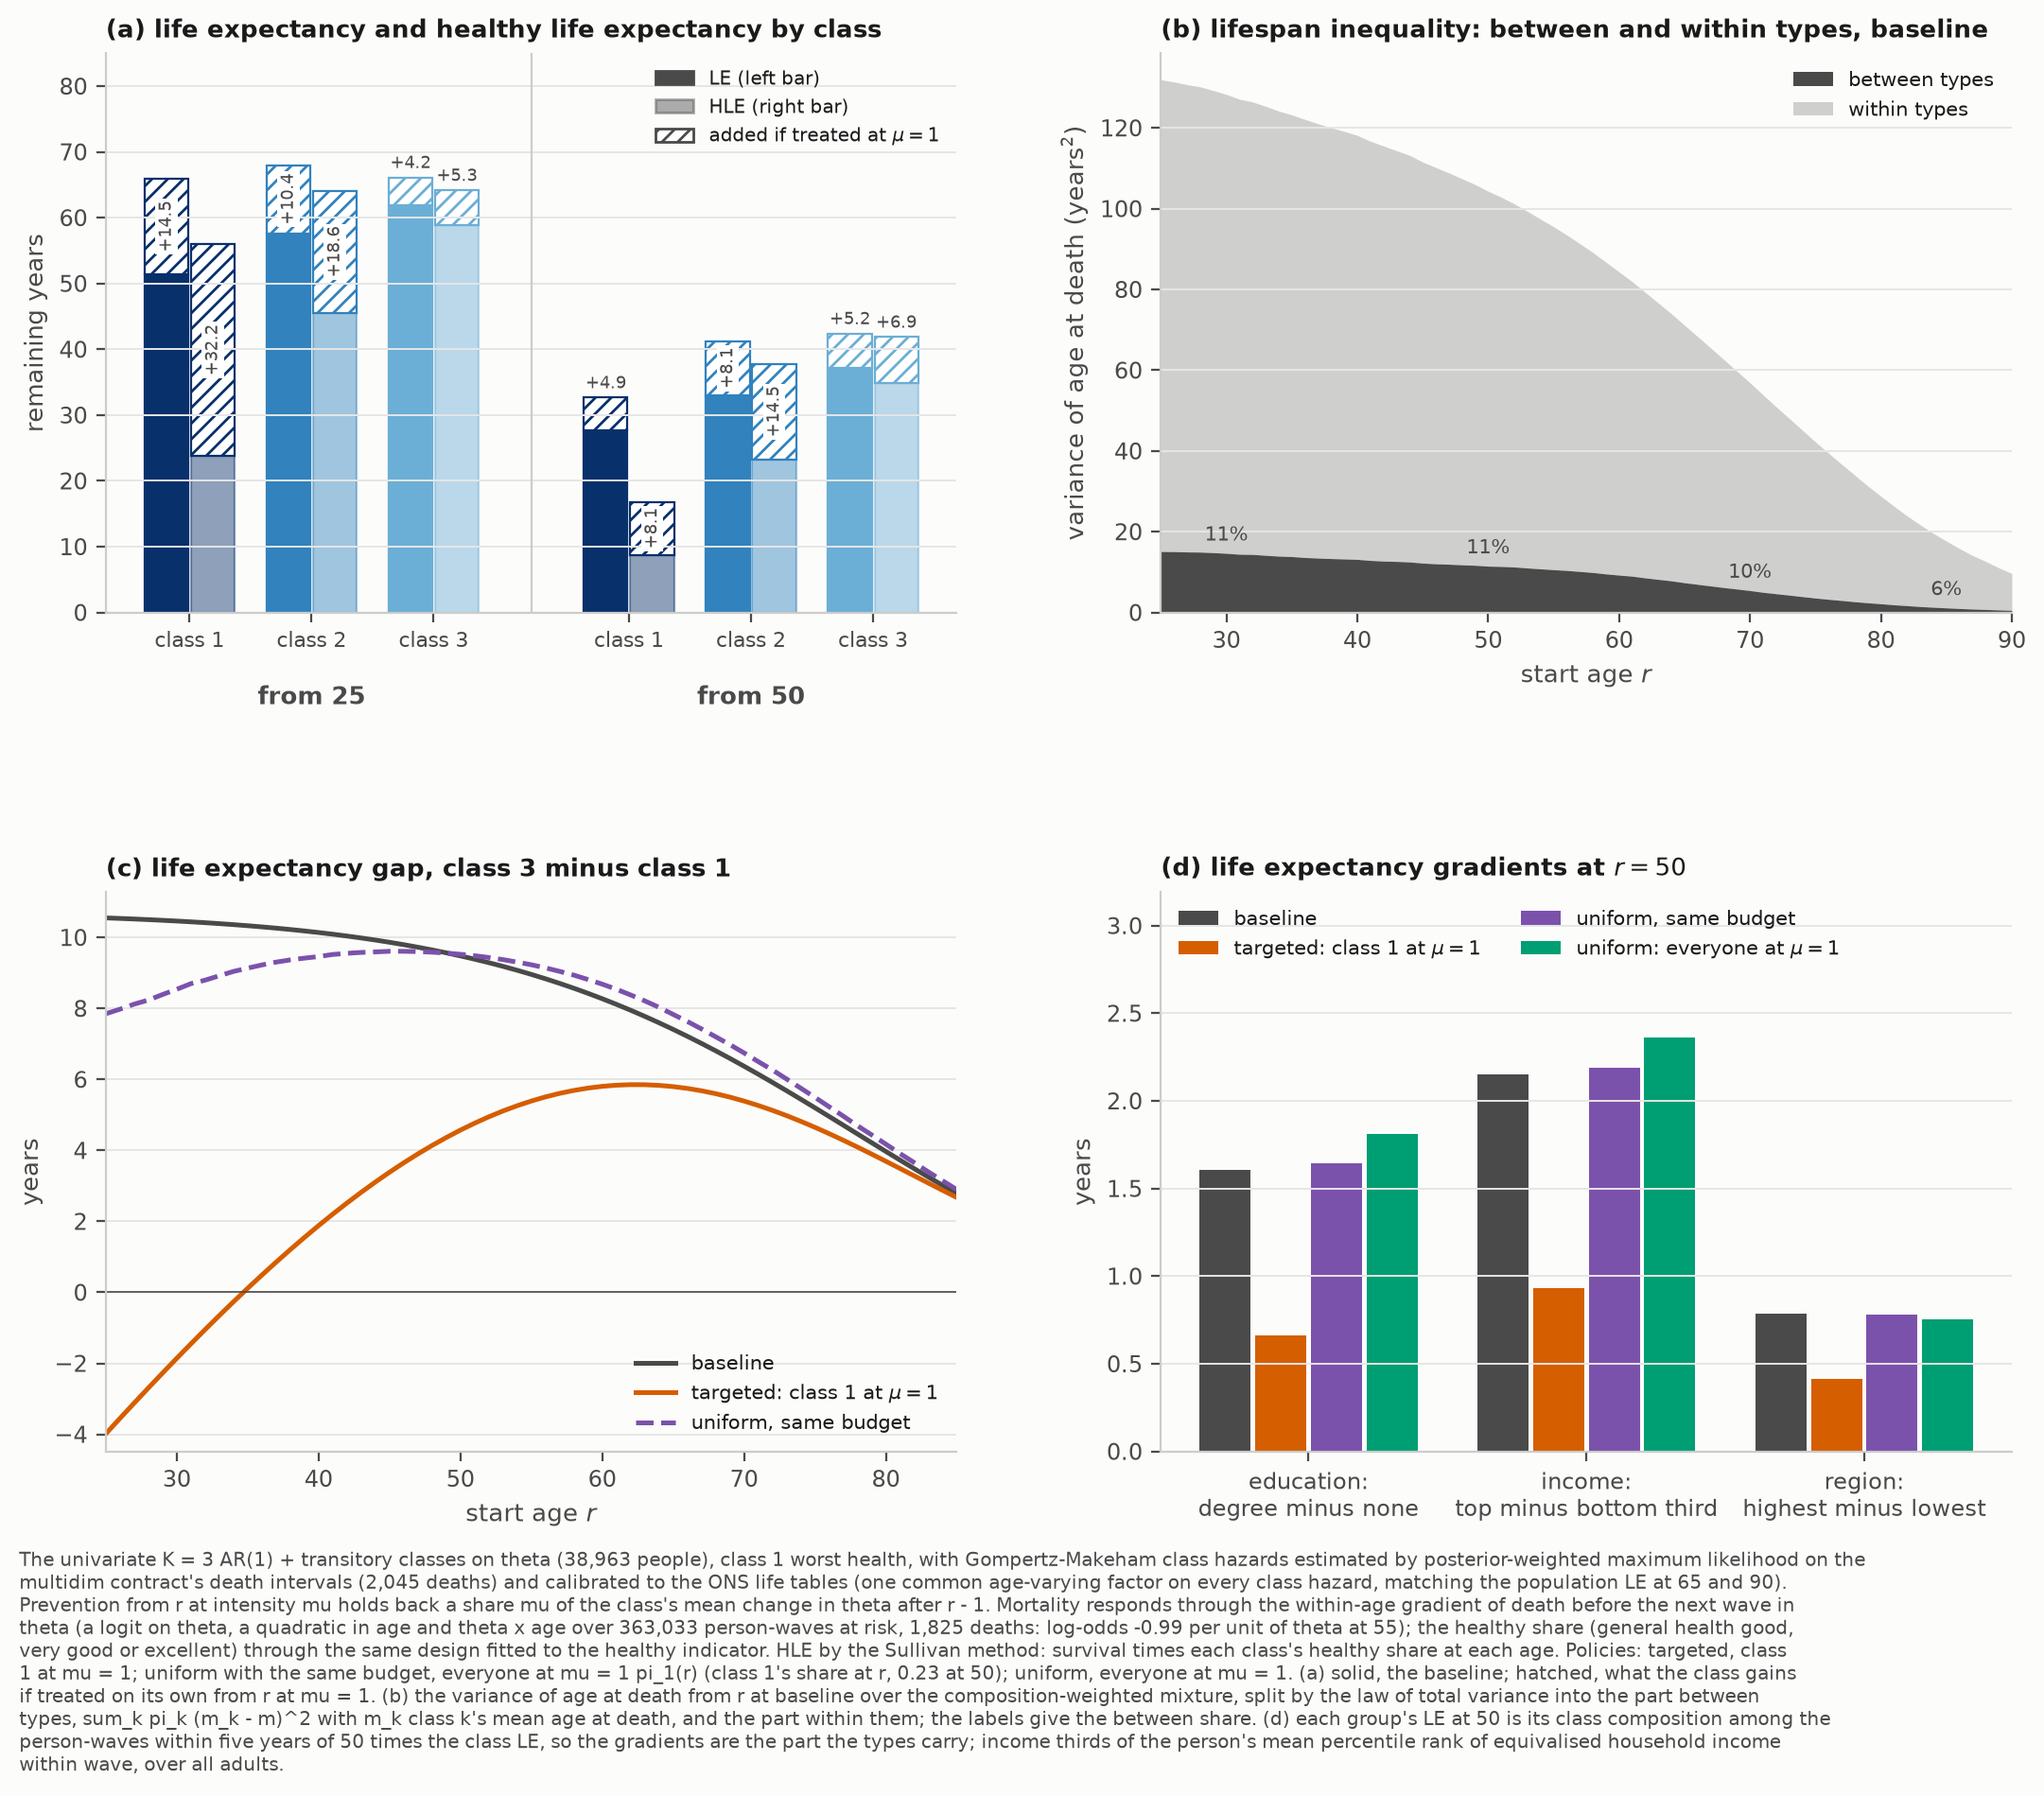
\includegraphics[width=\linewidth]{fig_prevention_le_uni_main.png}
	\caption{Targeted prevention in life years: (a) LE and HLE by class with gains if treated; (b) variance of age at death; (c) LE gap between best and worst class; (d) socioeconomic LE gradients.}
	\label{fig:prevle}
\end{figure}

\begin{itemize}
	\item Prevention adds more healthy years than years of life.
	\item Most lifespan inequality is within type (types explain about 11\%).
	\item Targeting the worst class from 50 halves the LE gap between types (9.5 to 4.6 years); the same budget spread evenly does not.
	\item It also more than halves the education and income LE gradients the types carry.
\end{itemize}

\open{gap between first-order and exact savings in the text; survival weighting and discounting; cost of a unit of $\mu$; within-class gradients; additive-prevention robustness; posterior uncertainty.}

%% =============================================================================
\section{Conclusions}
%% =============================================================================
\open{To be written.}

\bibliographystyle{plainnat}
\bibliography{references}

\clearpage
\appendix
\setcounter{page}{0}
\setcounter{figure}{0}
\setcounter{table}{0}
\setcounter{equation}{0}
\begin{center}
	{\LARGE\bf Appendices}
\end{center}
\medskip
\counterwithin{figure}{section}
\counterwithin{table}{section}
\counterwithin{equation}{section}
\renewcommand{\thefigure}{\thesection.\arabic{figure}}
\renewcommand{\thetable}{\thesection.\arabic{table}}
\renewcommand{\theequation}{\thesection.\arabic{equation}}

\section{Proofs and Additional Material for the Conceptual Framework}
\label{app:conceptual}
\open{Proofs and illustrative figures.}

\section{The Health Measure}
\label{app:health}

\subsection{Health Variables} \label{app:health_vars}
\begin{itemize}
	\item Item coding, impairment groups and the COND merge rule; 7.1\% of person-waves at the best answer on all items.
\end{itemize}

\begin{table}[H]
	\caption{Unconditional distribution by health variable}
	\label{tab:uncond_health_var}
	\centering\small
	\begin{tabular}{lr rrrrrrrrr}
		\toprule
		& $k$ & \multicolumn{9}{c}{share of person-waves, best category first (\%)} \\
		\cmidrule(l){3-11}
		GH & 5 & 13.29 & 33.33 & 31.71 & 15.58 & 6.10 & & & & \\
		PF & 5 & 65.13 & 11.66 & 11.82 & 4.60 & 6.79 & & & & \\
		RP & 9 & 52.18 & 6.85 & 12.77 & 4.55 & 11.57 & 2.68 & 4.76 & 1.20 & 3.44 \\
		BP & 5 & 53.72 & 25.24 & 9.14 & 8.26 & 3.64 & & & & \\
		LIM\_FL & 5 & 83.05 & 6.66 & 5.30 & 3.24 & 1.76 & & & & \\
		LIM\_SELF & 3 & 94.15 & 4.74 & 1.12 & & & & & & \\
		LIM\_SENS & 3 & 95.62 & 3.82 & 0.56 & & & & & & \\
		COND & 7 & 48.28 & 28.88 & 12.90 & 5.59 & 2.44 & 1.05 & 0.86 & & \\
		\bottomrule
	\end{tabular}
\end{table}

\subsection{The Graded Response Model} \label{app:grm_details}

\begin{table}[H]\centering\small
	\caption{Graded response model item parameters.}
	\label{tab:grm}
	\begin{tabular}{lrrl}
		\toprule
		Item & $k$ & $a$ & thresholds \\
		\midrule
		GH & 5 & 2.03 & $-2.10$\; $-0.98$\; $0.16$\; $1.45$ \\
		PF & 5 & 3.52 & $-1.73$\; $-1.38$\; $-0.80$\; $-0.40$ \\
		RP & 9 & 3.09 & $-2.20$\; $-2.03$\; $-1.56$\; $-1.37$\; $-0.81$\; $-0.64$\; $-0.23$\; $-0.03$ \\
		BP & 5 & 2.31 & $-2.35$\; $-1.50$\; $-0.99$\; $-0.09$ \\
		LIM\_FL & 5 & 3.38 & $-2.49$\; $-1.94$\; $-1.46$\; $-1.07$ \\
		LIM\_SELF & 3 & 2.43 & $-2.95$\; $-1.99$ \\
		LIM\_SENS & 3 & 1.36 & $-4.49$\; $-2.85$ \\
		COND & 7 & 1.18 & $-4.61$\; $-3.90$\; $-3.12$\; $-2.26$\; $-1.25$\; $0.11$ \\
		\bottomrule
	\end{tabular}
\end{table}

\begin{figure}[H]\centering
	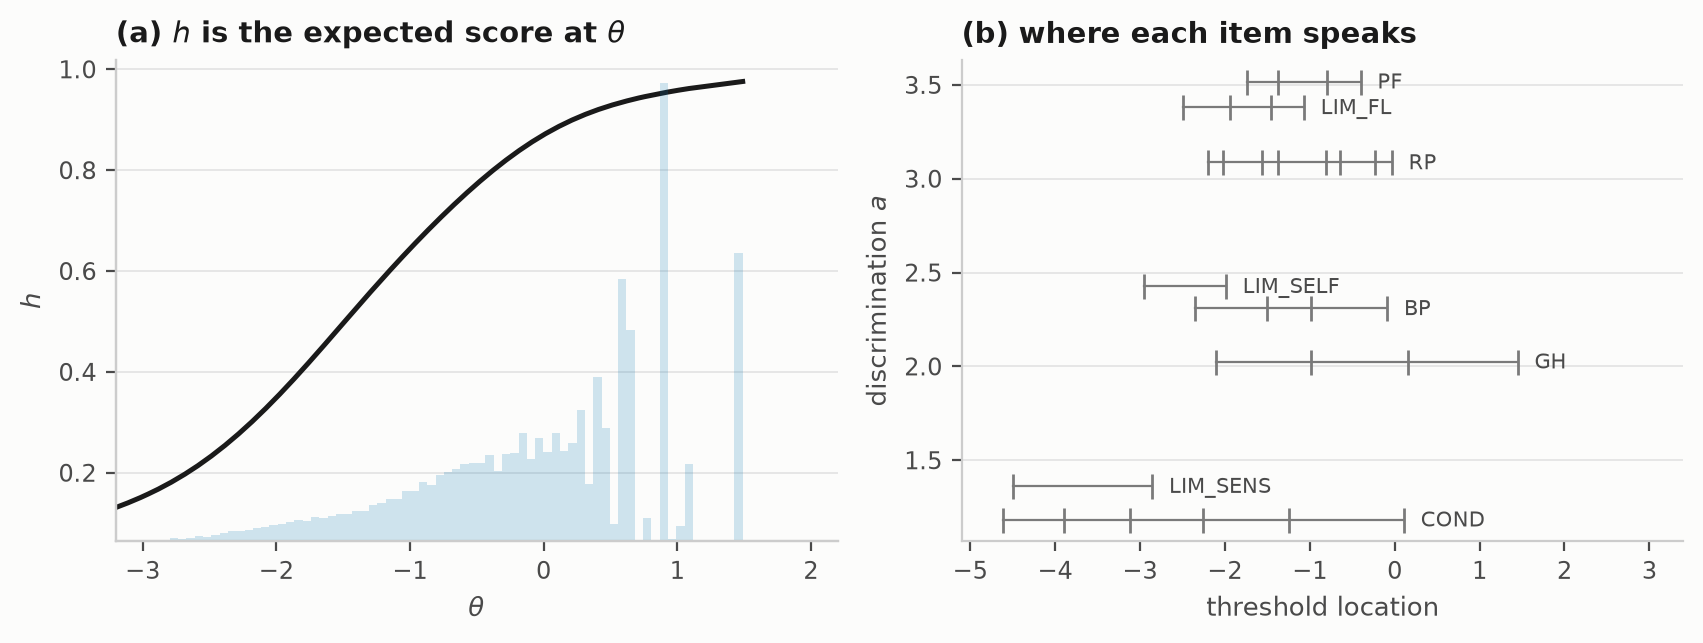
\includegraphics[width=\linewidth]{fig_health_scale.png}
	\caption{(a) The map from $\theta$ to $h$; (b) item discriminations against thresholds.}
	\label{fig:h_theta_comp}
\end{figure}

\begin{table}[H]\centering\small
	\begin{tabular}{lrrrr}
\toprule
 & $\theta$ & $h$ & frailty index (negated) & log frailty (negated) \\
\midrule
UKHLS PCS & 0.903 & 0.935 & 0.859 & 0.837 \\
UKHLS MCS & 0.274 & 0.266 & 0.232 & 0.228 \\
chronic count (negated) & 0.576 & 0.587 & 0.785 & 0.763 \\
Spearman, vs $\theta$ & 1.000 & 1.000 & 0.920 & 0.920 \\
\bottomrule
\end{tabular}

	\caption{Correlations of the four measures with comparison metrics.}
	\label{tab:corr}
\end{table}

\subsection{The Frailty Indices} \label{app:frailty}
\begin{itemize}
	\item 31 equal-weight deficits (SF-12 physical items, eight impairment areas, 17 conditions); differs from \citet{hosseini2022} in deficits, self-rated health and treatment of zeros.
\end{itemize}

\section{The Cost Proxy}
\label{app:cost}

\subsection{Inputs}
\begin{table}[H]\centering\small
	\caption{UKHLS variables behind the cost proxy, waves 7--15.}
	\label{tab:costvars}
	\begin{tabular}{llp{6.4cm}}
		\toprule
		Quantity & Source & Coverage \\
		\midrule
		Any admission & \texttt{hosp} & complete for respondents \\
		Nights in hospital & \texttt{hospd} & all admitted; median 3, mean 7.5, max 300 \\
		Maternity flag & \texttt{hospch} & 12.7\% of admissions; left out \\
		GP visits, banded & \texttt{hl2gp} & 0 / 1--2 / 3--5 / 6--10 / more than 10 \\
		Out-patient attendances, banded & \texttt{hl2hop} & same bands \\
		\bottomrule
	\end{tabular}
\end{table}

\subsection{Sensitivity of the Convexity}
\begin{itemize}
	\item All twelve costing variants are convex ($t$ 17--36); long-stay pricing moves the sickest-to-healthiest ratio most.
\end{itemize}
\begin{figure}[H]
	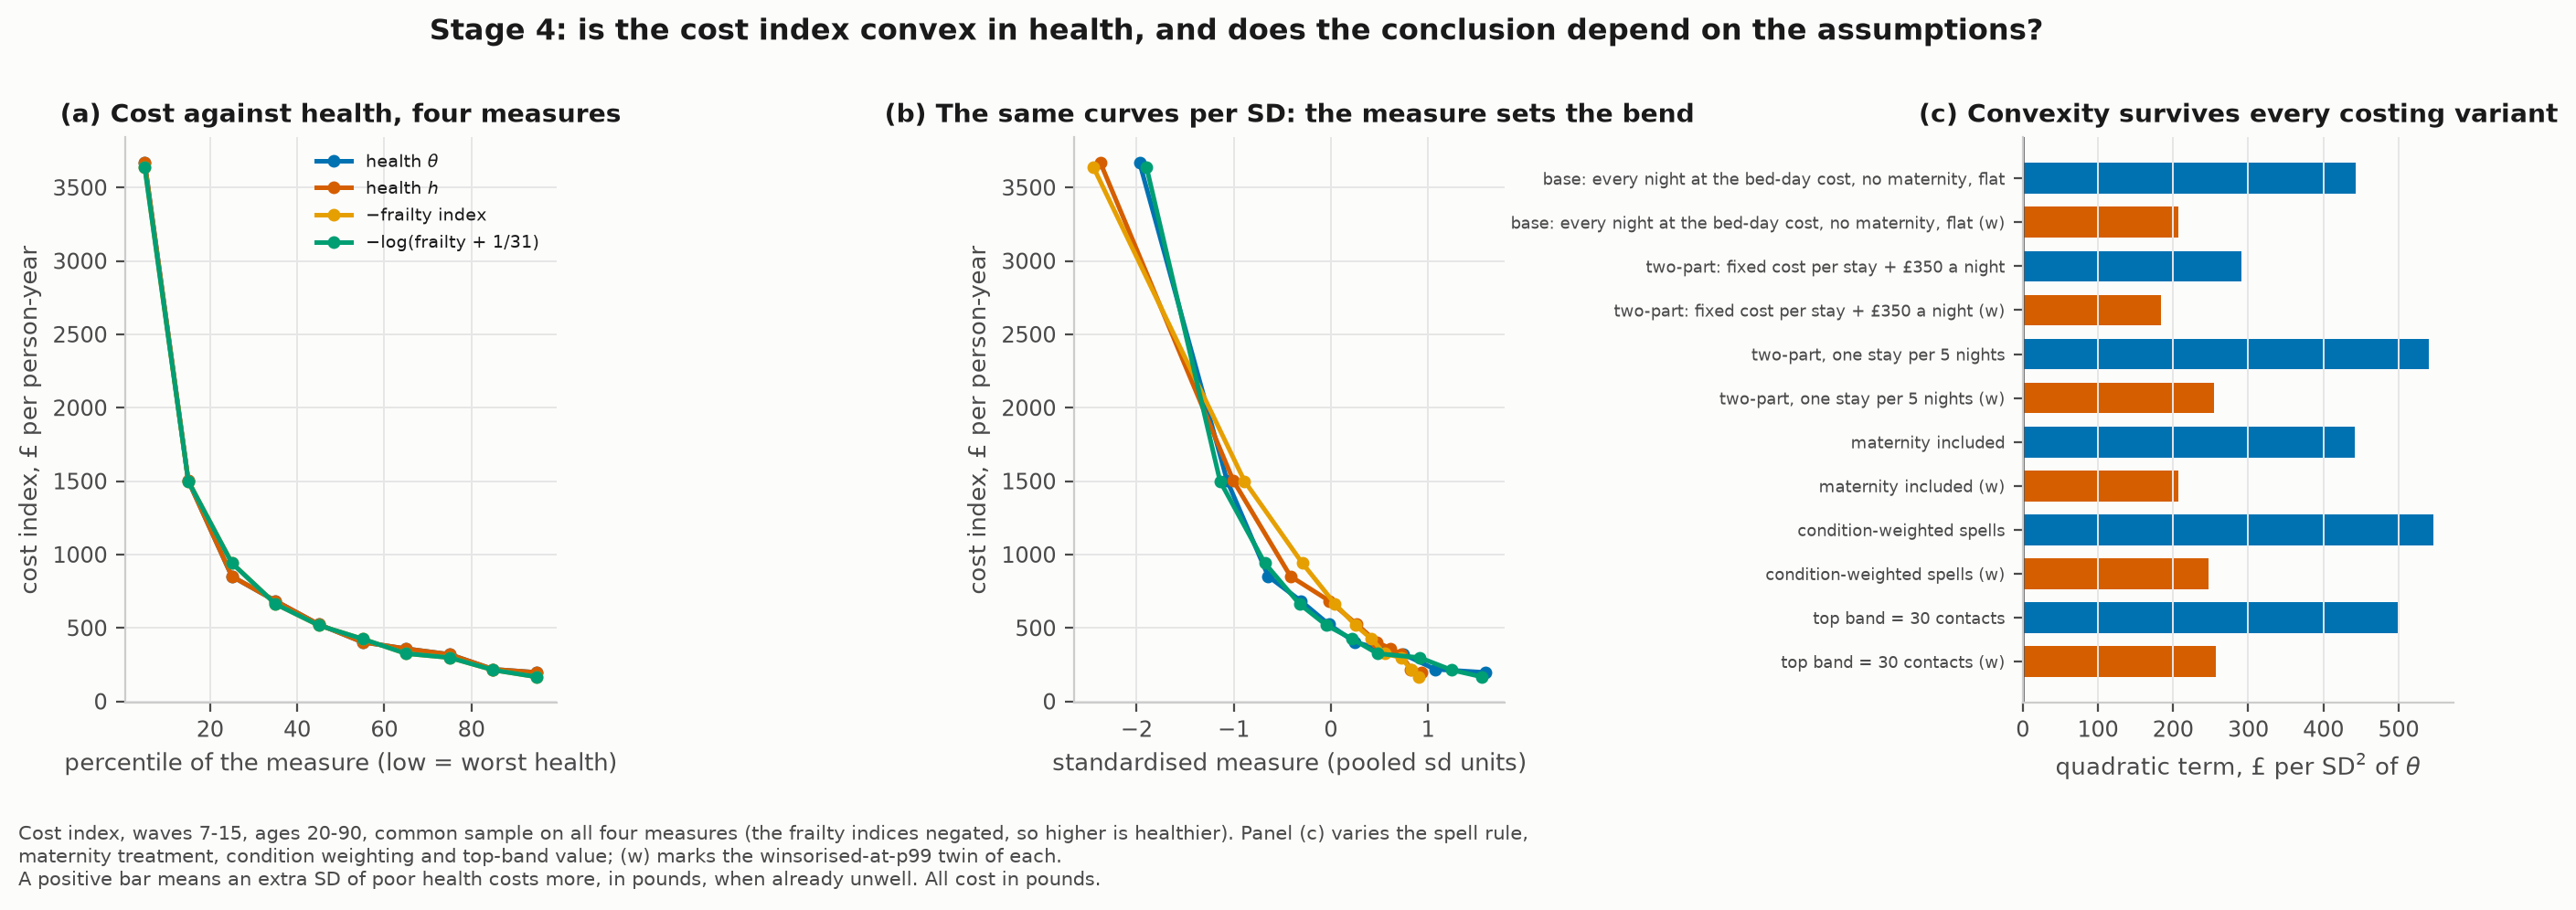
\includegraphics[width=\linewidth]{fig_cost_convexity}
	\caption{Cost against the four measures, and sensitivity of the convexity to each costing assumption.}
	\label{fig:costconvex}
\end{figure}

\subsection{Validation against Published Profiles}
\label{app:costval}
\begin{itemize}
	\item Concentration passes; level undershoots as expected; age profile too flat (3$\times$ vs 7$\times$), so not for cost-by-age projections. The health gradient is strong.
\end{itemize}
\begin{figure}[H]\centering
	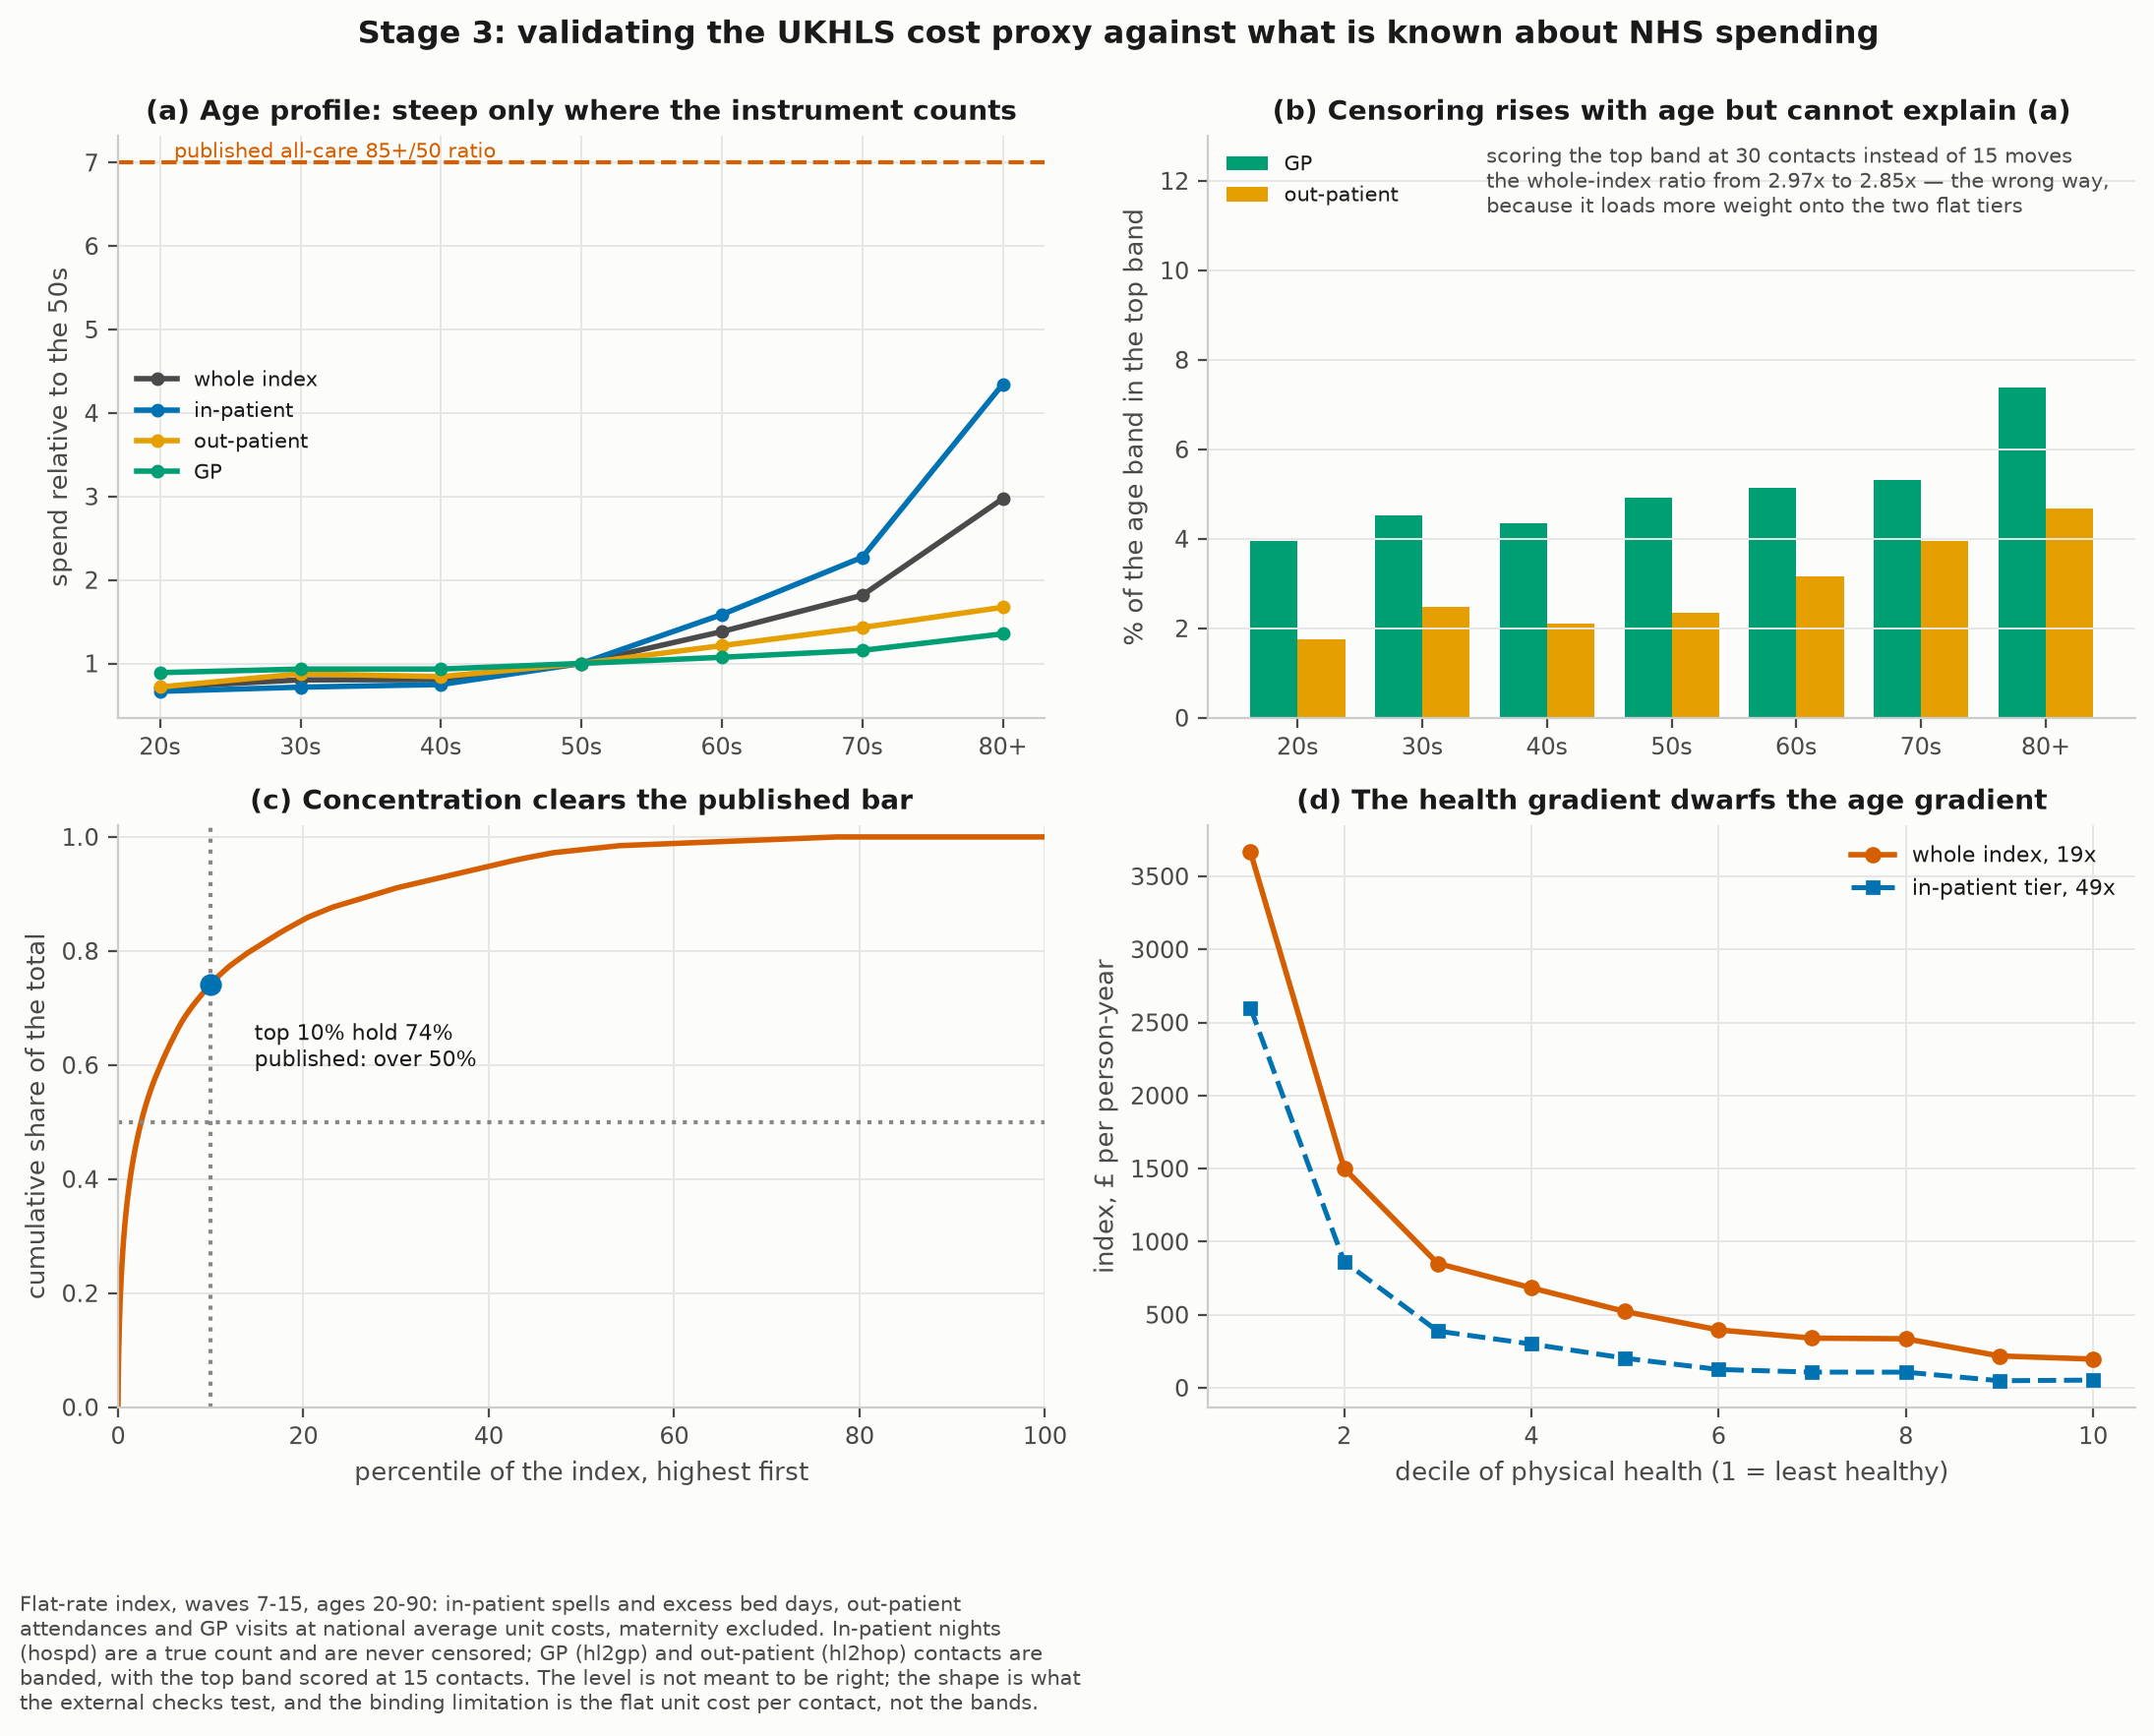
\includegraphics[width=\linewidth]{fig_cost_validation}
	\caption{Validation: age profile, top-coding, concentration, health gradient.}
	\label{fig:costval}
\end{figure}

\section{Additional Descriptive Results} \label{app:descriptive}

\subsection{Robustness of the Moments}
\label{app:moments_robust}
\begin{itemize}
	\item Balanced rows sit lower but keep the first-year drop and the slope signs.
	\item Cost itself is almost entirely a one-period draw: the in-the-moment part of the bill that prevention cannot reach.
\end{itemize}
\begin{figure}[H]\centering
	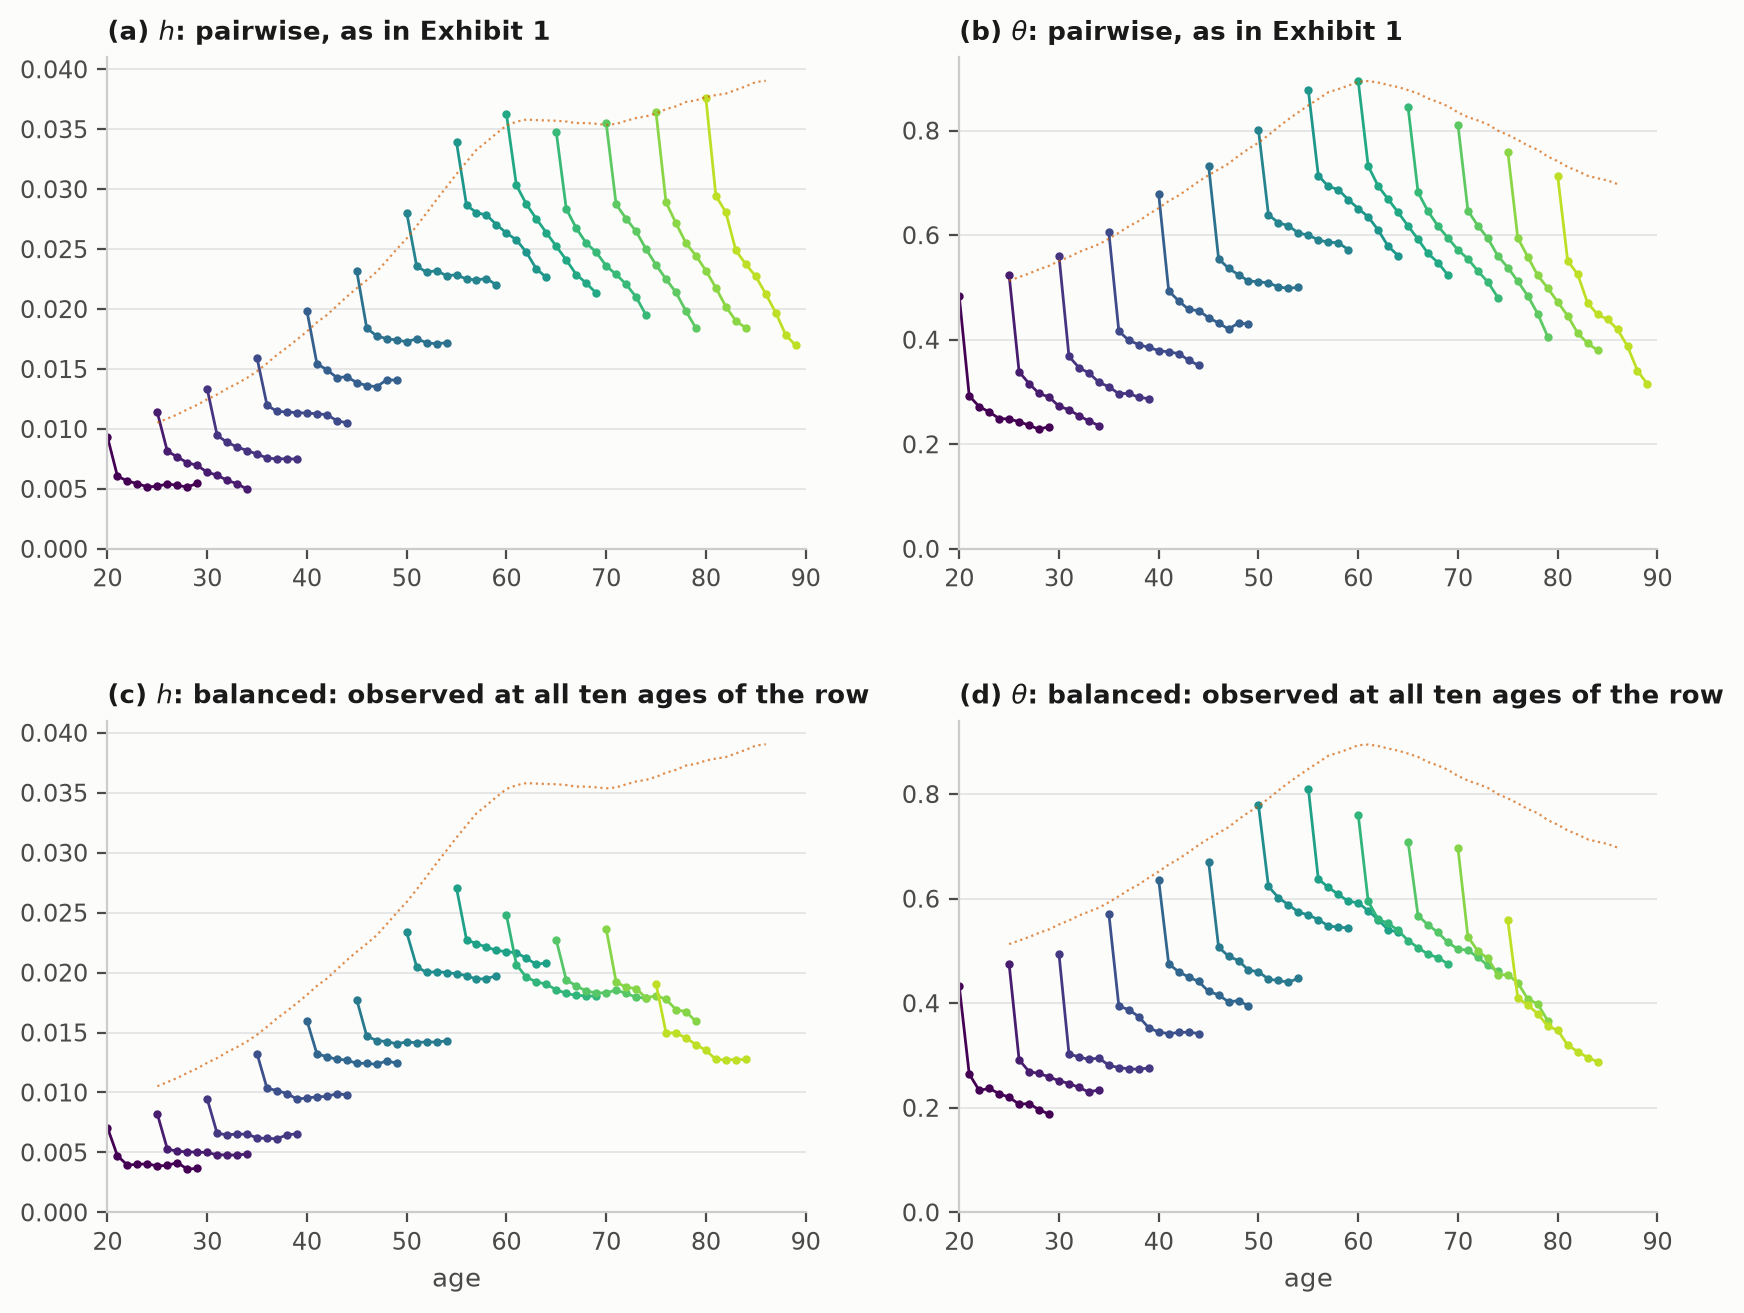
\includegraphics[width=\linewidth]{fig_exhibit1_balanced.png}
	\caption{Covariance rows on pairwise (top) and balanced (bottom) samples.}
	\label{fig:ex1balanced}
\end{figure}
\begin{figure}[H]\centering
	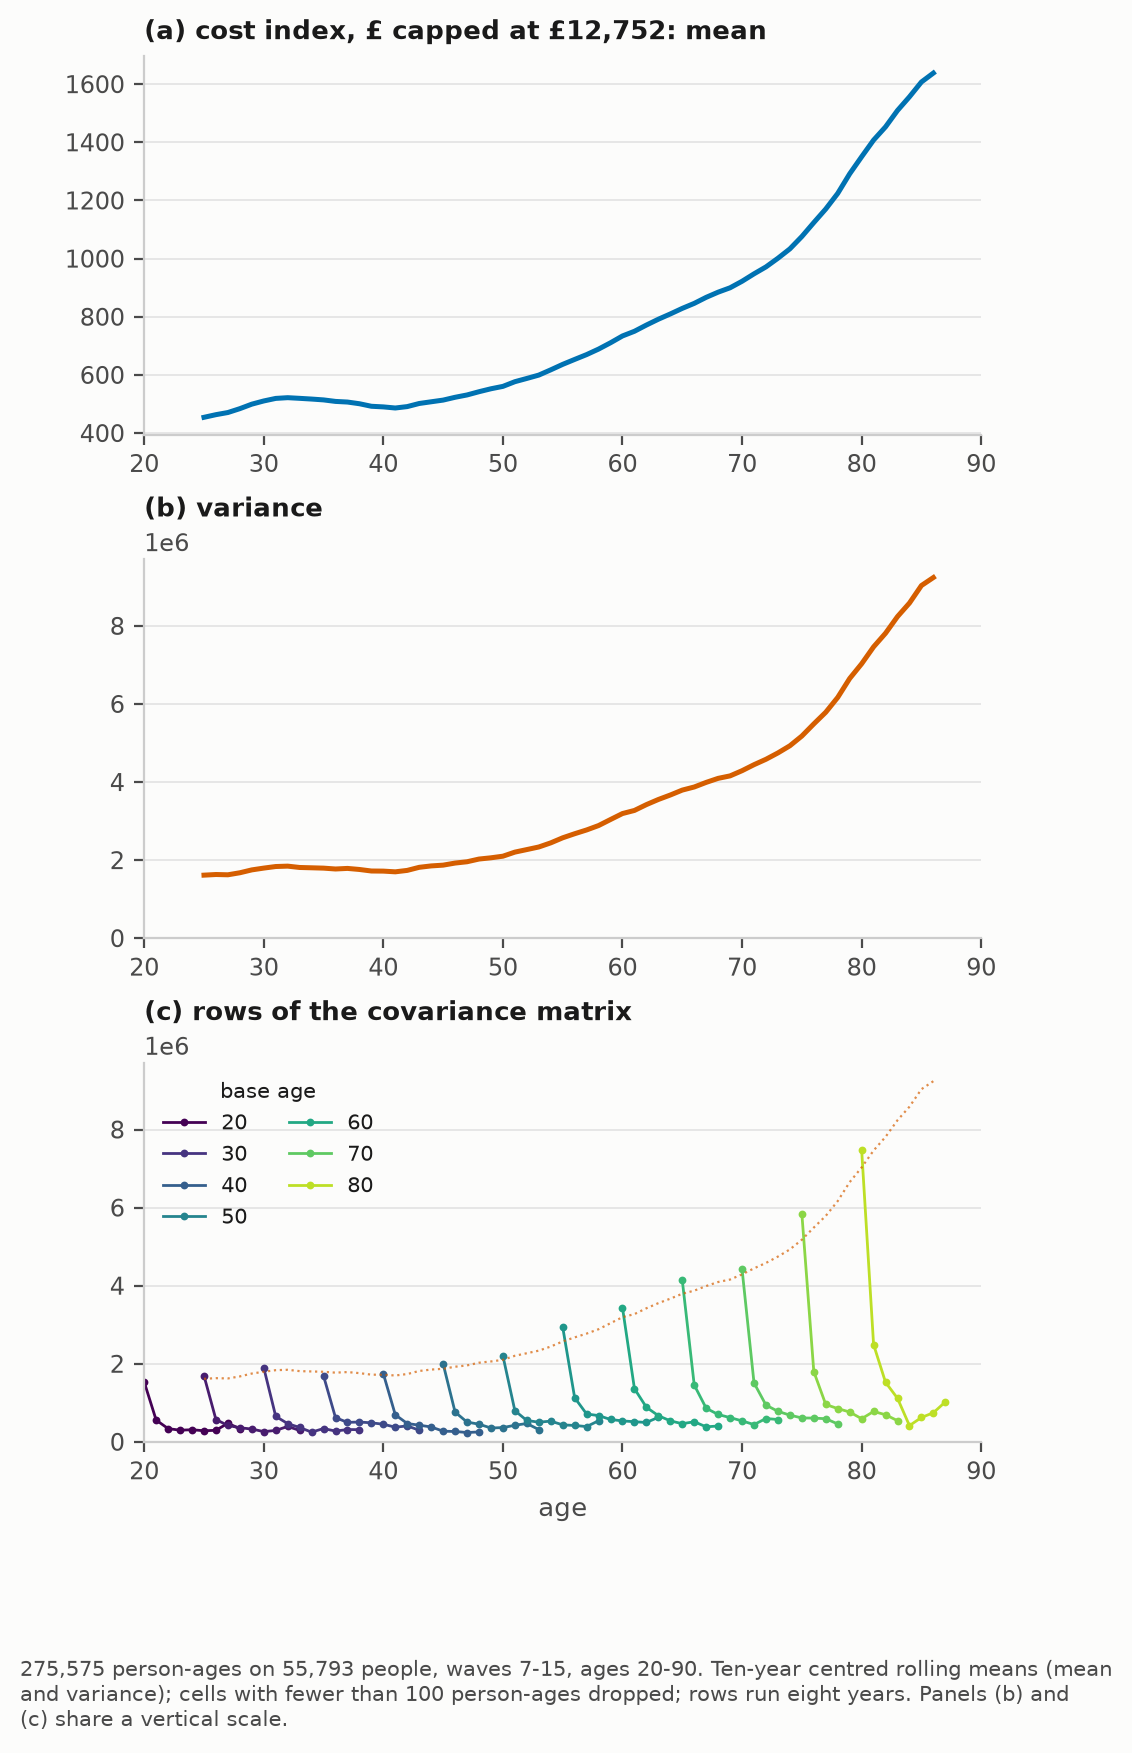
\includegraphics[width=0.55\linewidth]{fig_exhibit1_cost.png}
	\caption{The cost index through the moments of Figure~\ref{fig:exhibit1}.}
	\label{fig:ex1cost}
\end{figure}

\subsection{The Linear Approximation}
\label{app:linear_robust}
\begin{figure}[H]\centering
	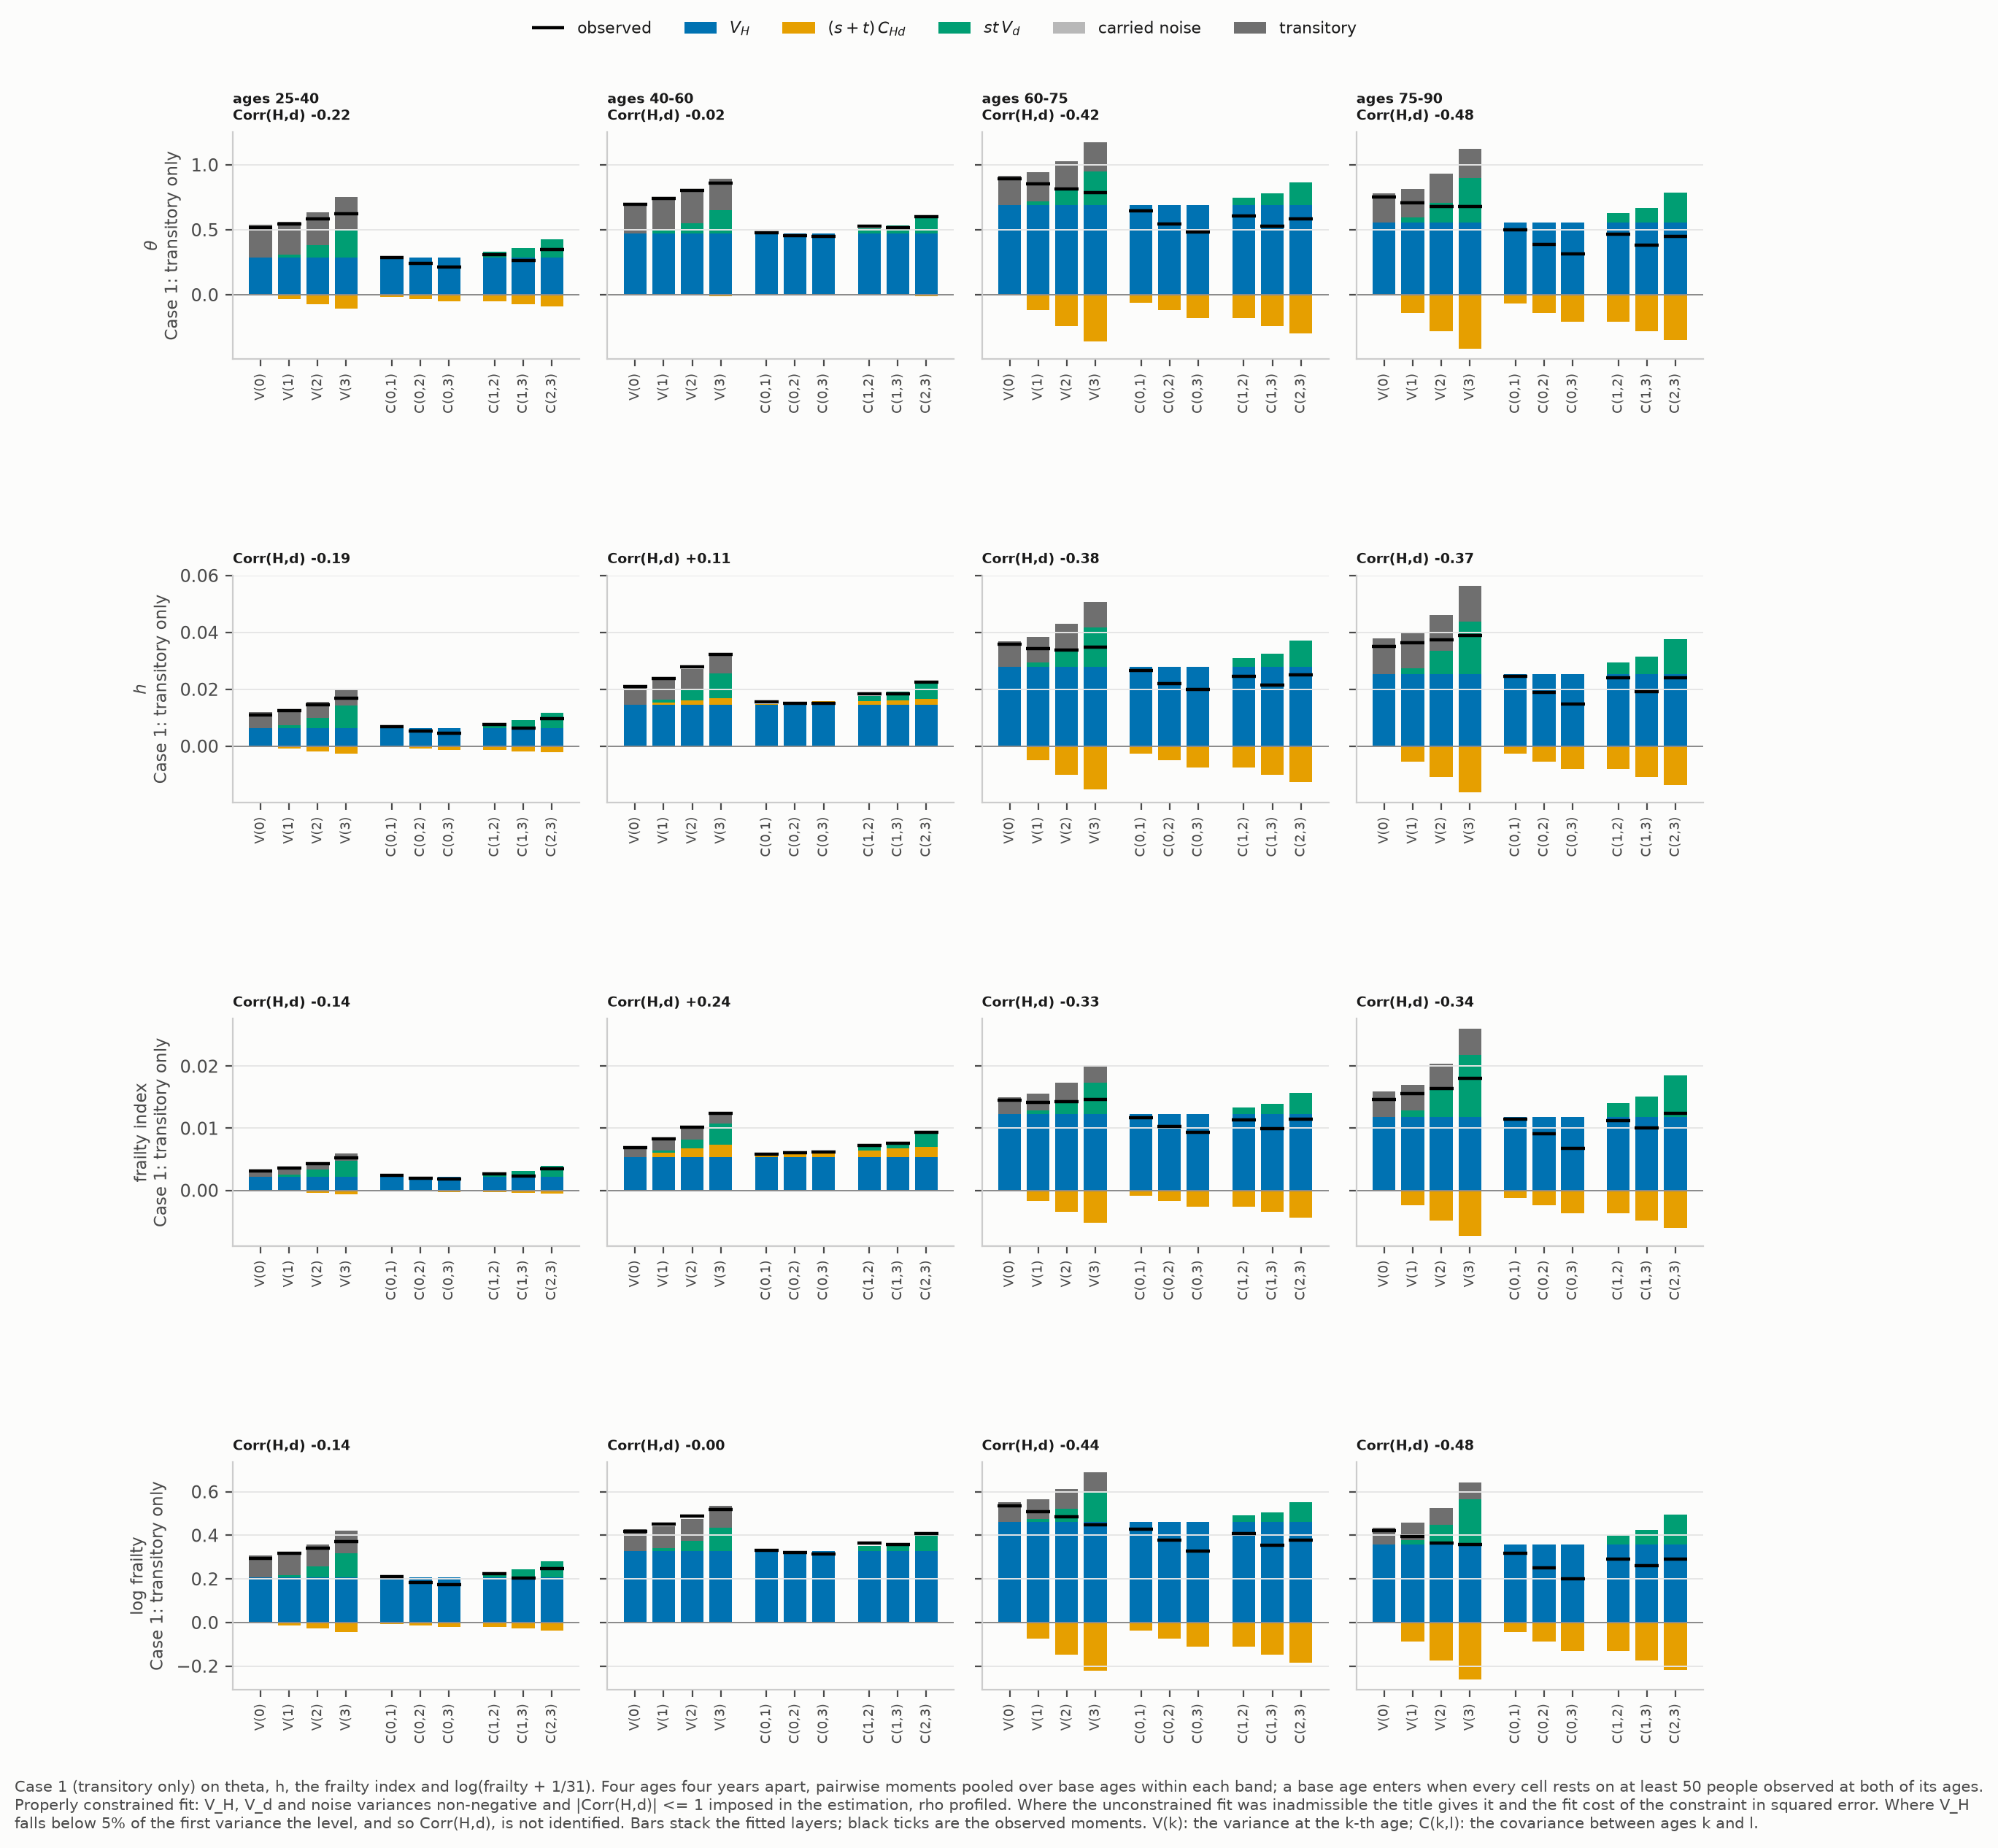
\includegraphics[width=\linewidth]{fig_exhibit2_case1.png}
	\caption{Figure~\ref{fig:ex2main} under Case~1 (transitory only), on all four measures.}
	\label{fig:ex2case1}
\end{figure}
\begin{figure}[H]\centering
	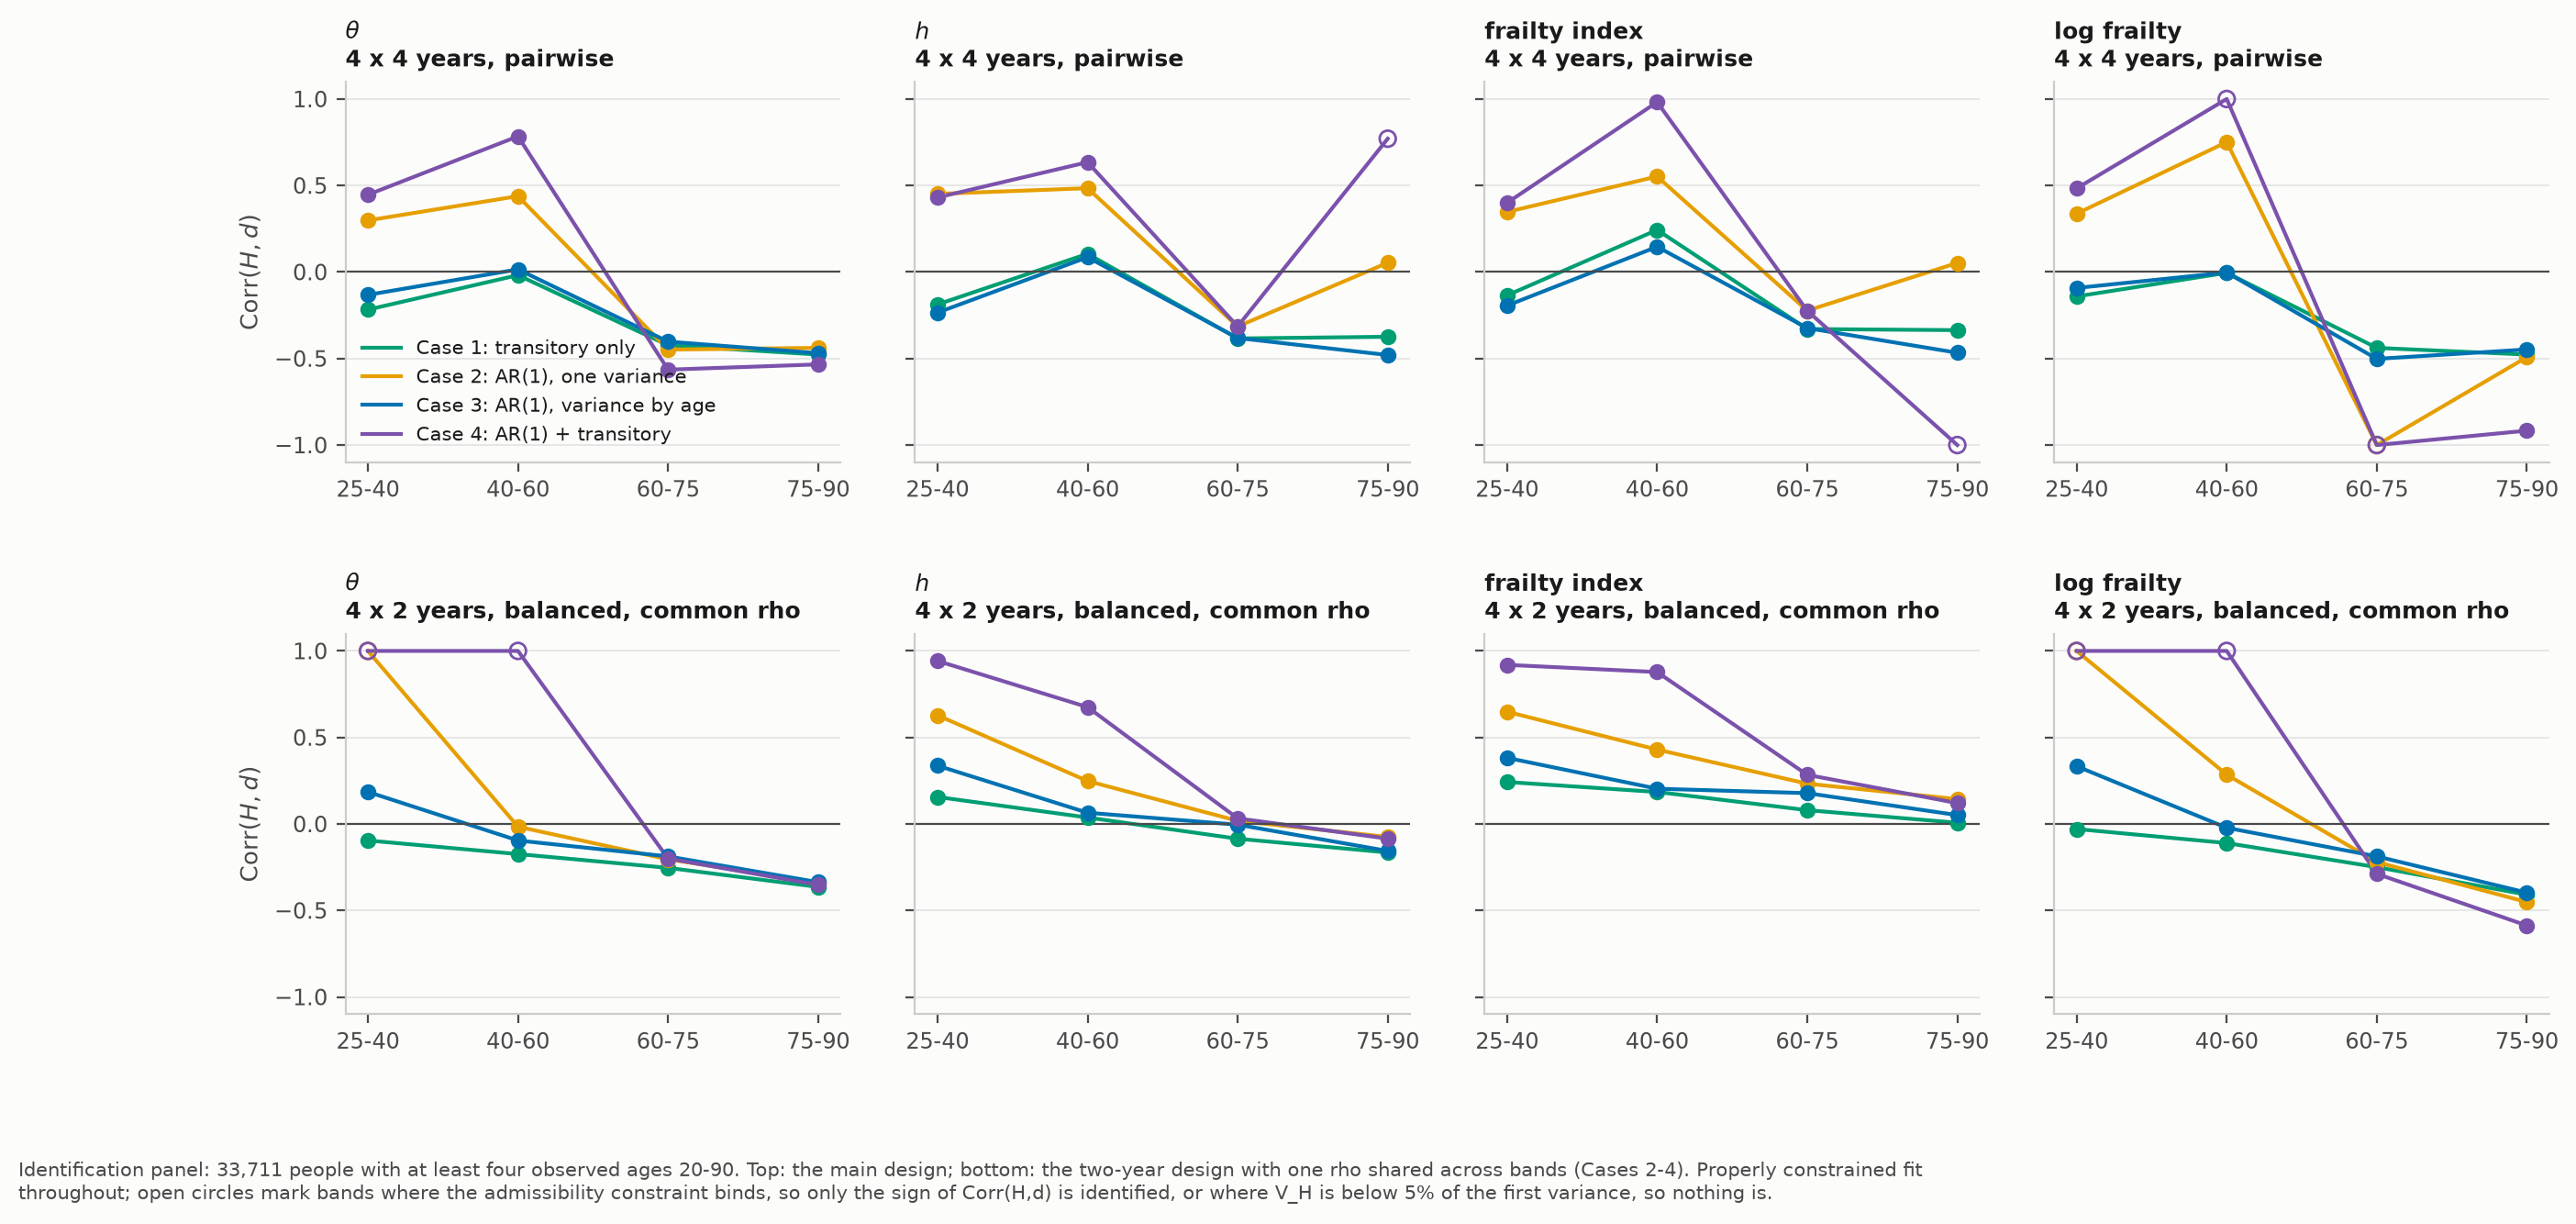
\includegraphics[width=\linewidth]{fig_exhibit2_corr.png}
	\caption{Implied $\Corr(H,d)$ by age band under Cases 1--4, all measures, two designs.}
	\label{fig:ex2corr}
\end{figure}
\begin{figure}[H]\centering
	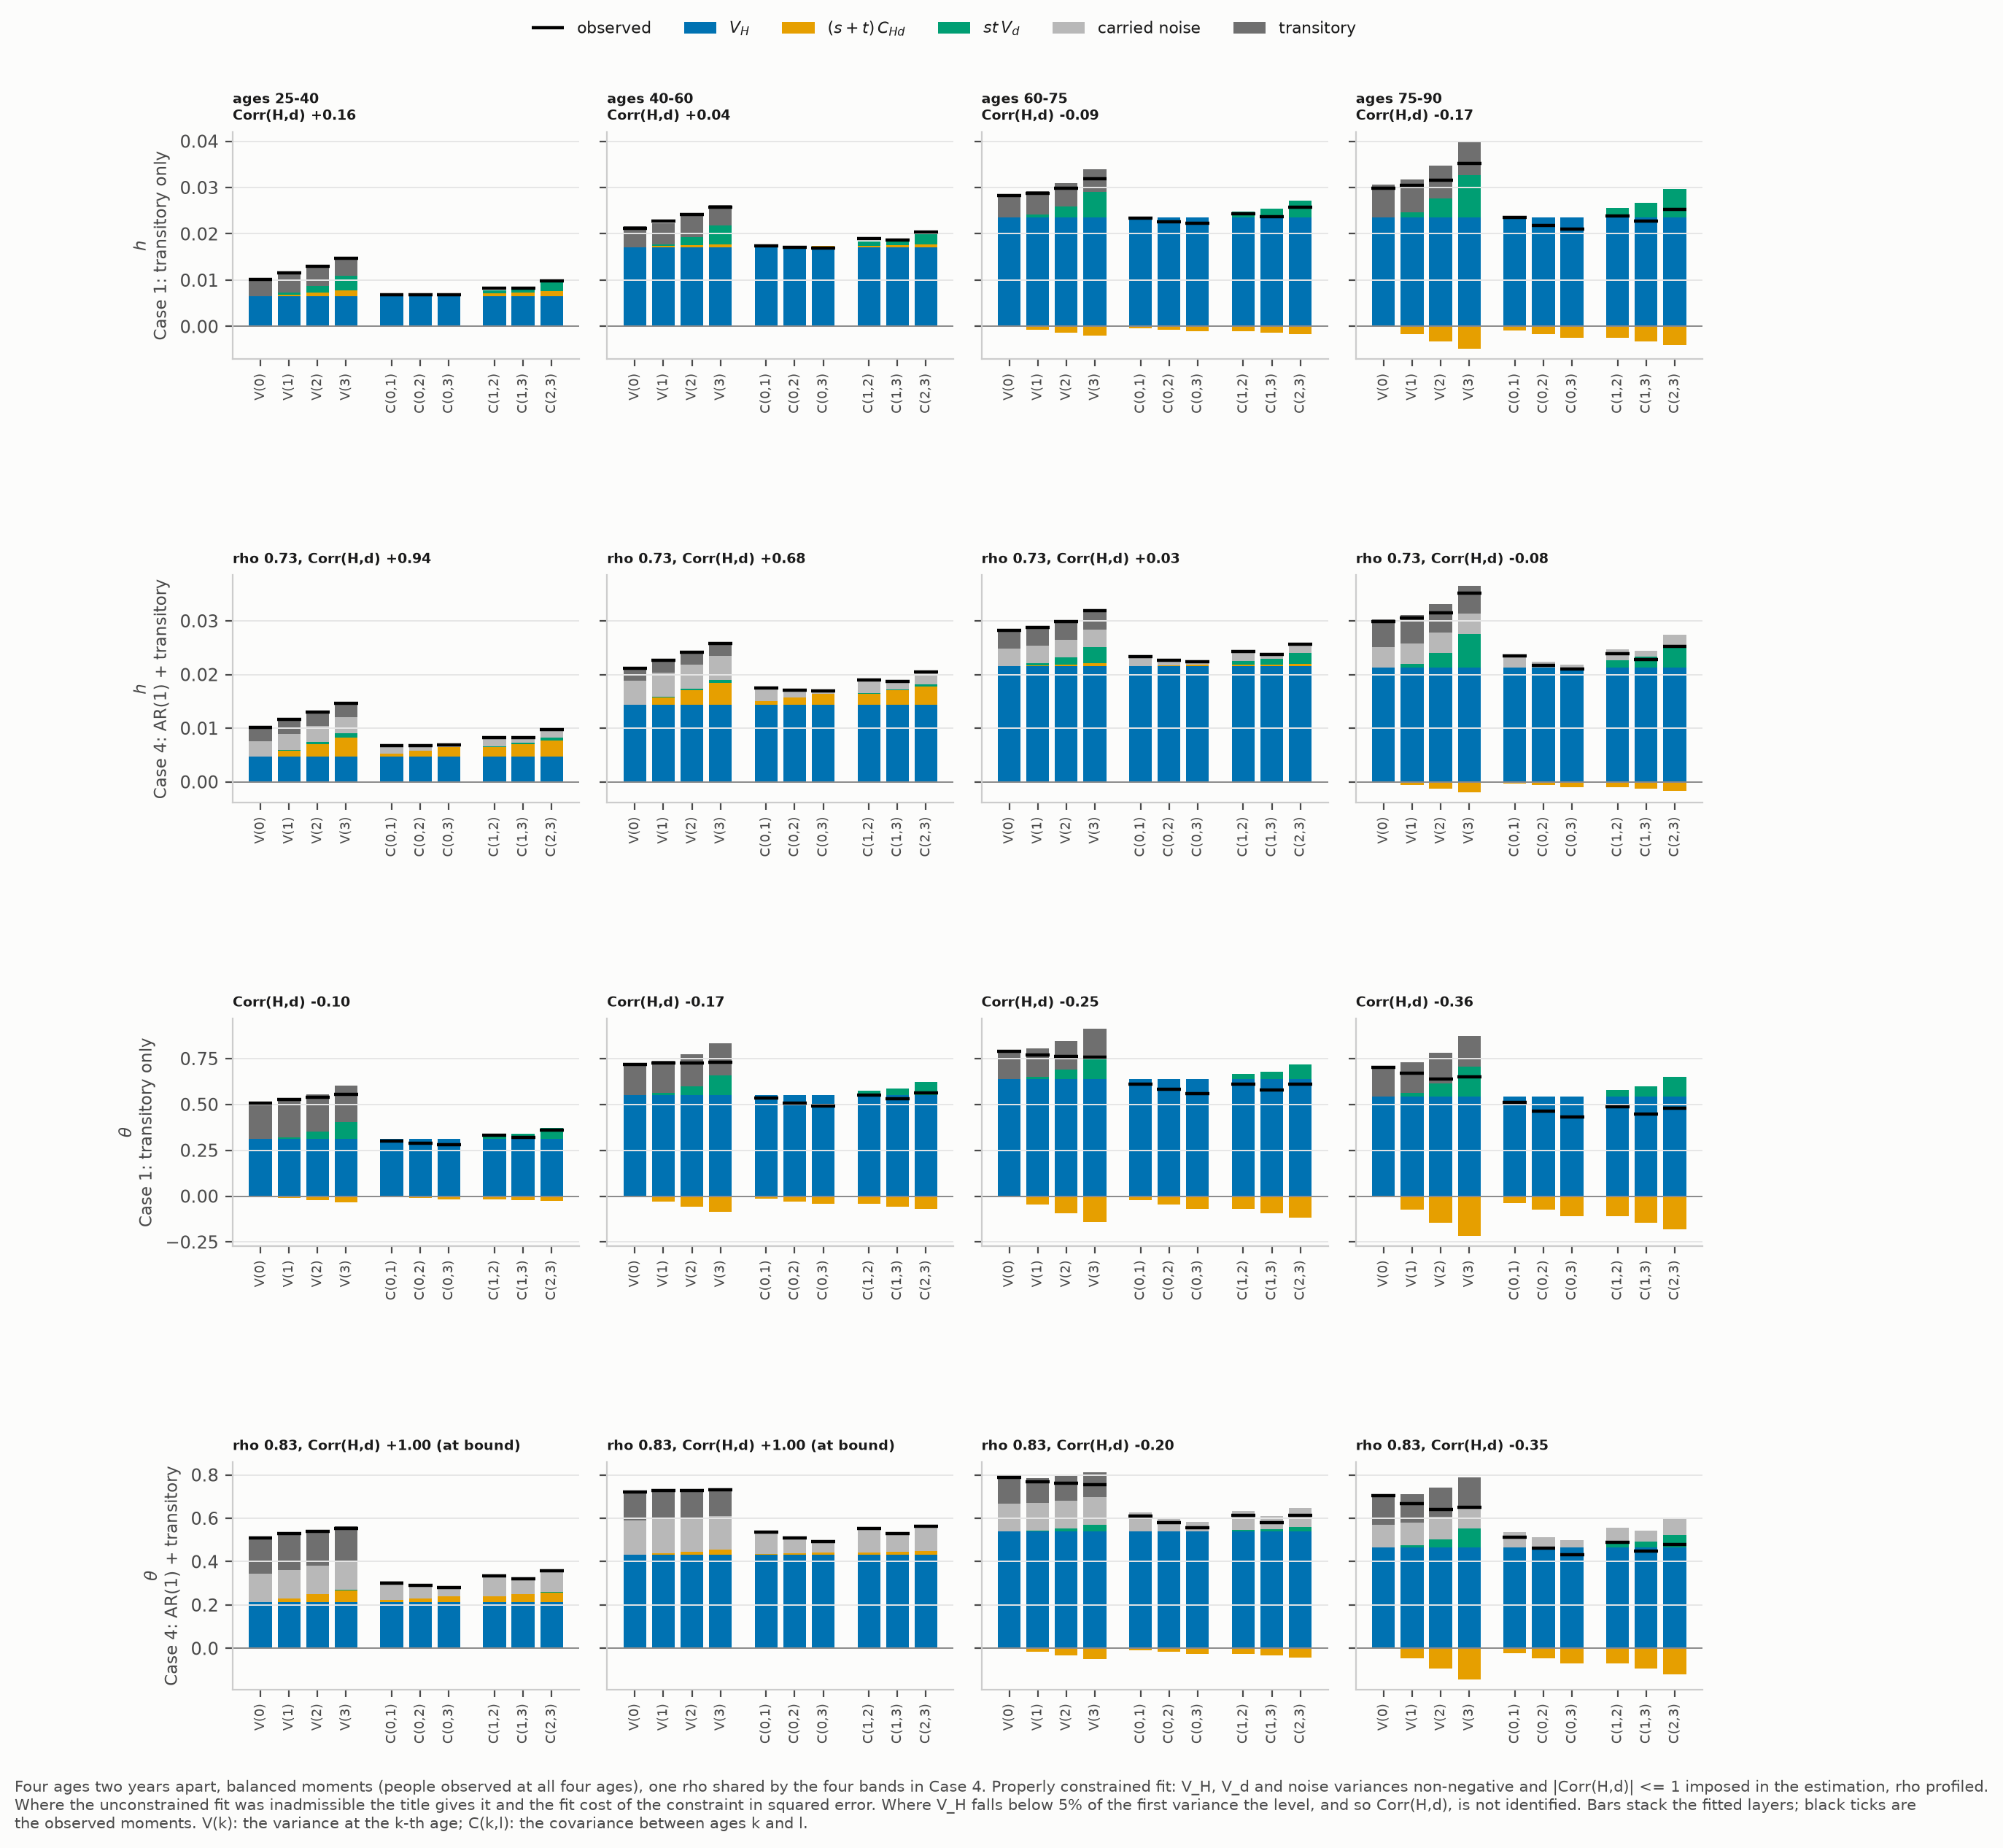
\includegraphics[width=\linewidth]{fig_exhibit2_2y.png}
	\caption{Figure~\ref{fig:ex2main} on the two-year balanced design.}
	\label{fig:ex2twoyear}
\end{figure}

\section{Additional K-Means Results} \label{app:kmeans}

\subsection{The Types on Predicted Cost}
\label{app:clusters_predcost}
\begin{figure}[H]\centering
	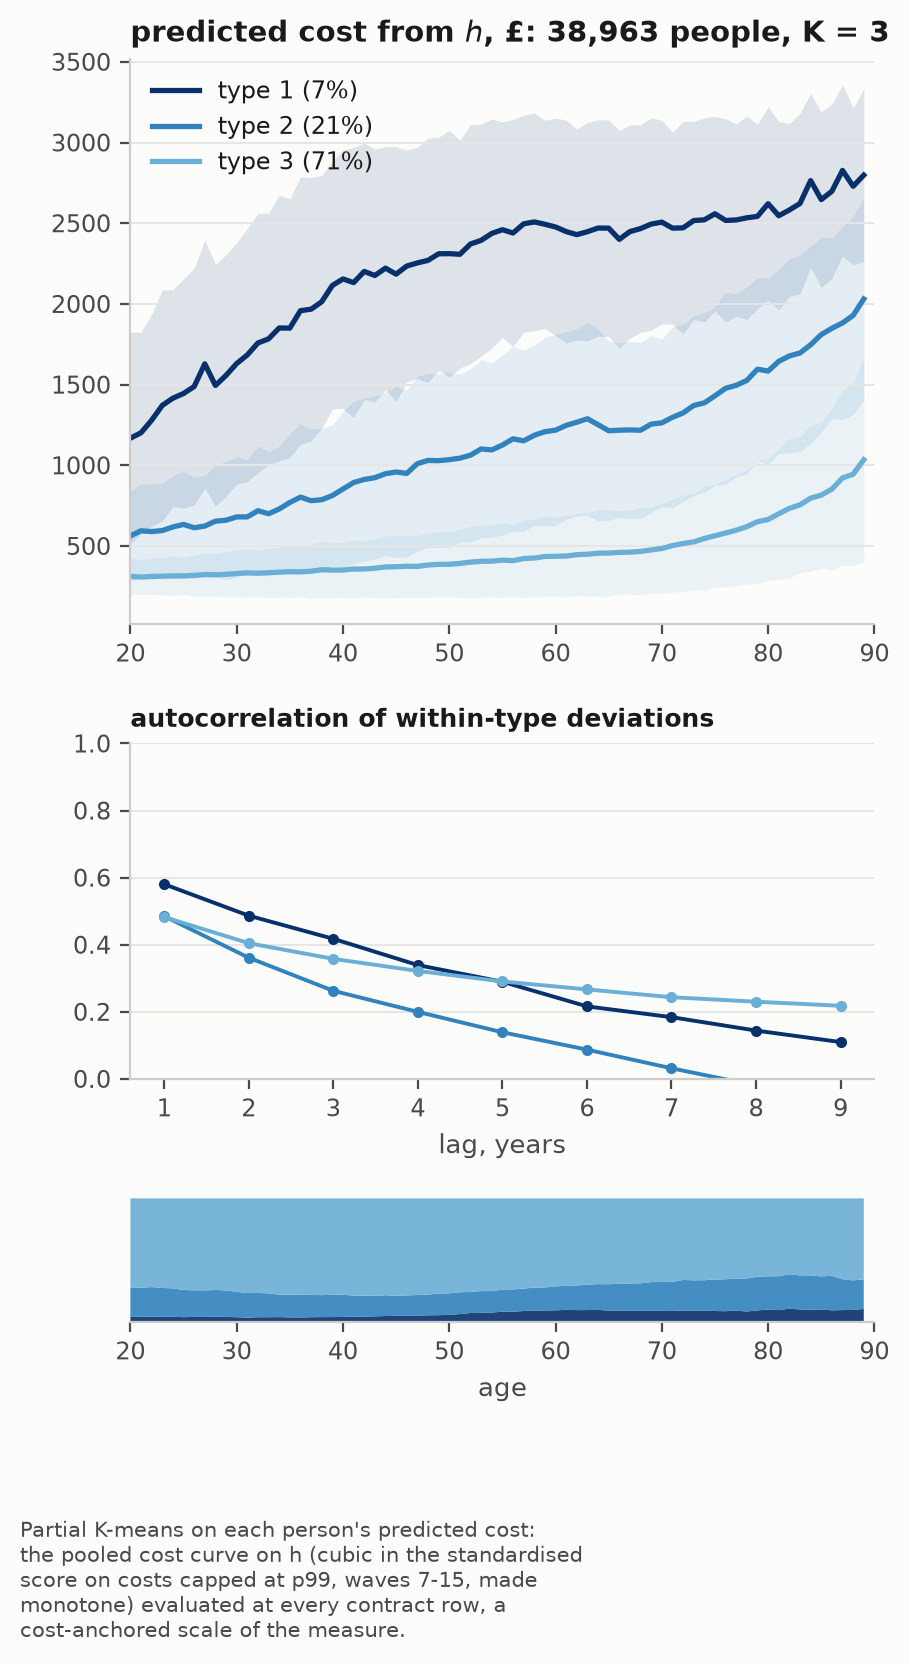
\includegraphics[width=0.55\linewidth]{fig_clusters_predcost.png}
	\caption{Partial K-means on predicted cost; lands with the $h$ types (ARI 0.65).}
	\label{fig:clusterspredcost}
\end{figure}

\subsection{Types over Age Windows}
\label{app:kmeans_windows}
\begin{itemize}
	\item K-means is more stable across windows than the mixture, but only because it is insensitive to where the decline happens.
\end{itemize}
\begin{figure}[H]\centering
	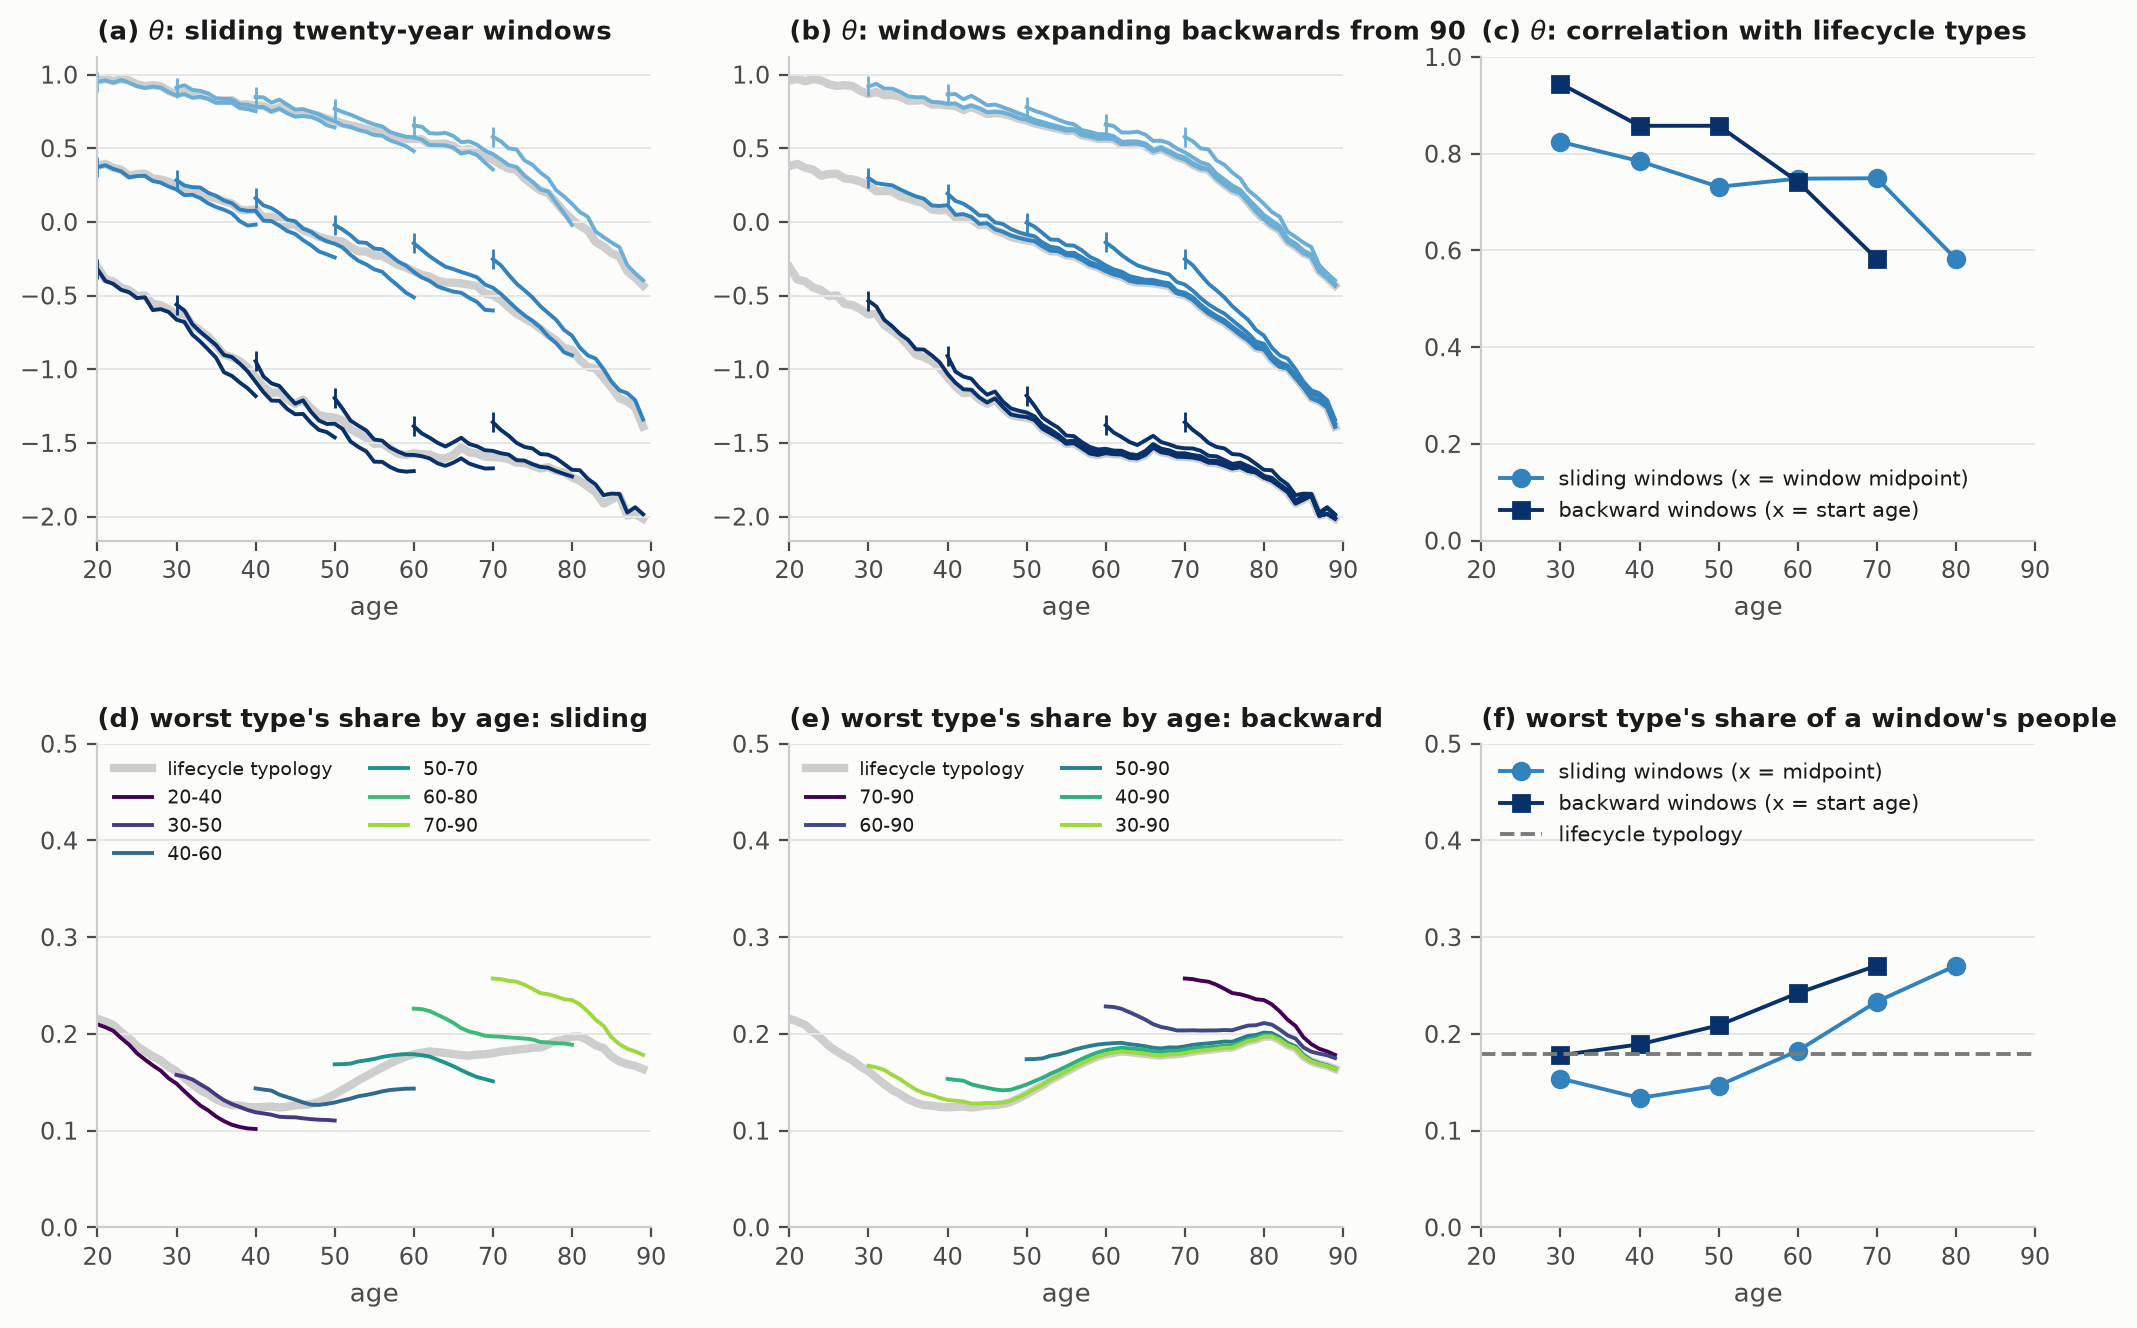
\includegraphics[width=\linewidth]{fig_windows.png}
	\caption{As Figure~\ref{fig:windows}, for partial K-means.}
	\label{fig:windows_kmeans}
\end{figure}

\section{Additional Bayesian Results} \label{app:bayesian}

\subsection{The Worst Type by Method and Number of Classes}
\label{app:worsttype}
\begin{itemize}
	\item The error structure changes the worst type's path, not its membership; more classes tighten it without changing its shape.
\end{itemize}
\begin{figure}[H]\centering
	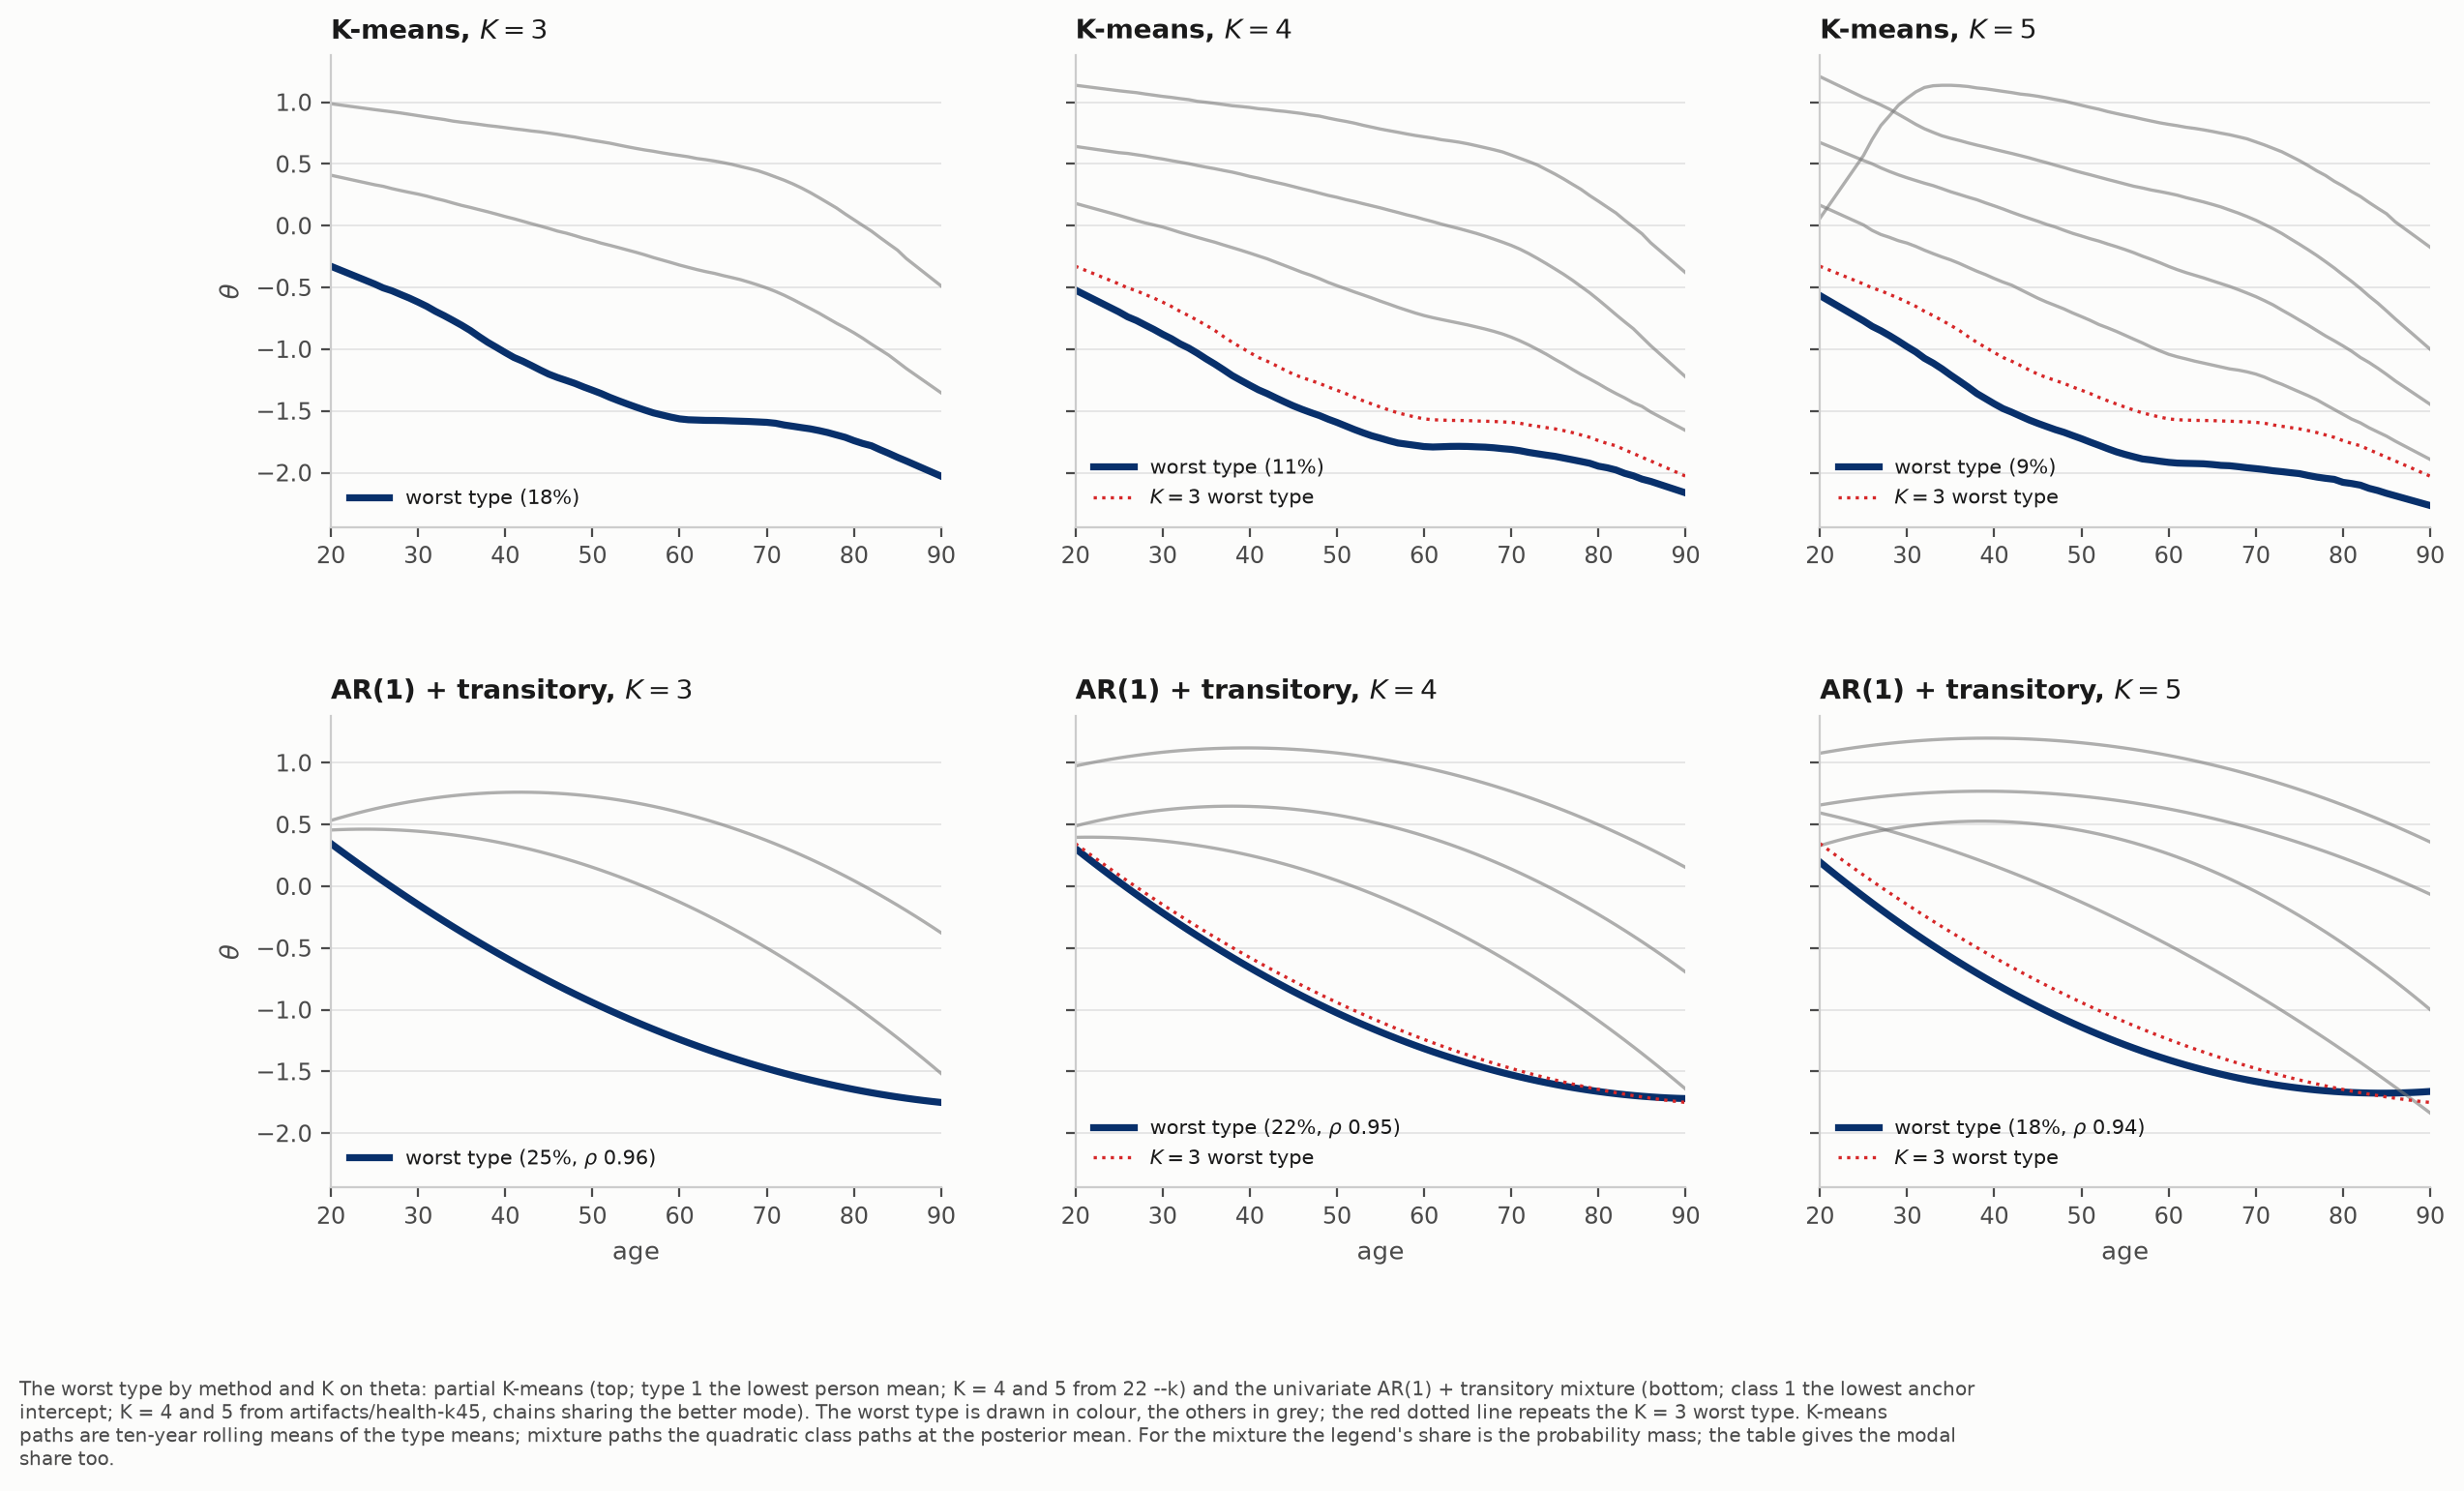
\includegraphics[width=0.9\linewidth]{fig_worst_type_by_K.png}
	\caption{The worst type under K-means and the persistent--transitory mixture, $K=3,4,5$.}
	\label{fig:worsttype}
\end{figure}
\begin{table}[H]\centering\scriptsize\setlength{\tabcolsep}{2.5pt}
	\begin{tabular}{llrrrrrrrrr}
\toprule
method & $K$ & share & $\theta_{20}$ & $\theta_{50}$ & $\theta_{80}$ & slope to 50 & sd at 50 & $\rho$ & of $K{=}3$ worst & worst under other \\
\midrule
K-means & 3 & 18\% & -0.33 & -1.33 & -1.74 & -0.033 & 0.66 &  & 100\% & 85\% \\
 & 4 & 11\% & -0.52 & -1.59 & -1.95 & -0.036 & 0.59 &  & 63\% & 92\% \\
 & 5 & 9\% & -0.57 & -1.72 & -2.08 & -0.039 & 0.55 &  & 48\% & 94\% \\
\addlinespace
AR(1) + transitory & 3 & 18\% (25\%) & 0.35 & -0.94 & -1.65 & -0.043 & 0.81 & 0.96 & 100\% & 83\% \\
 & 4 & 15\% (22\%) & 0.31 & -1.03 & -1.66 & -0.044 & 0.80 & 0.95 & 84\% & 67\% \\
 & 5 & 14\% (18\%) & 0.20 & -1.14 & -1.67 & -0.045 & 0.79 & 0.94 & 76\% & 57\% \\
\bottomrule
\end{tabular}

	\caption{The worst type by method and $K$.}
	\label{tab:worsttype}
\end{table}

\subsection{Which Type Drives the Level--Slope Reversal?}
\label{app:reversal}
\begin{itemize}
	\item The worst type's own convergence carries nearly all the negative covariance after 60, also with within-person slopes.
\end{itemize}
\begin{figure}[H]\centering
	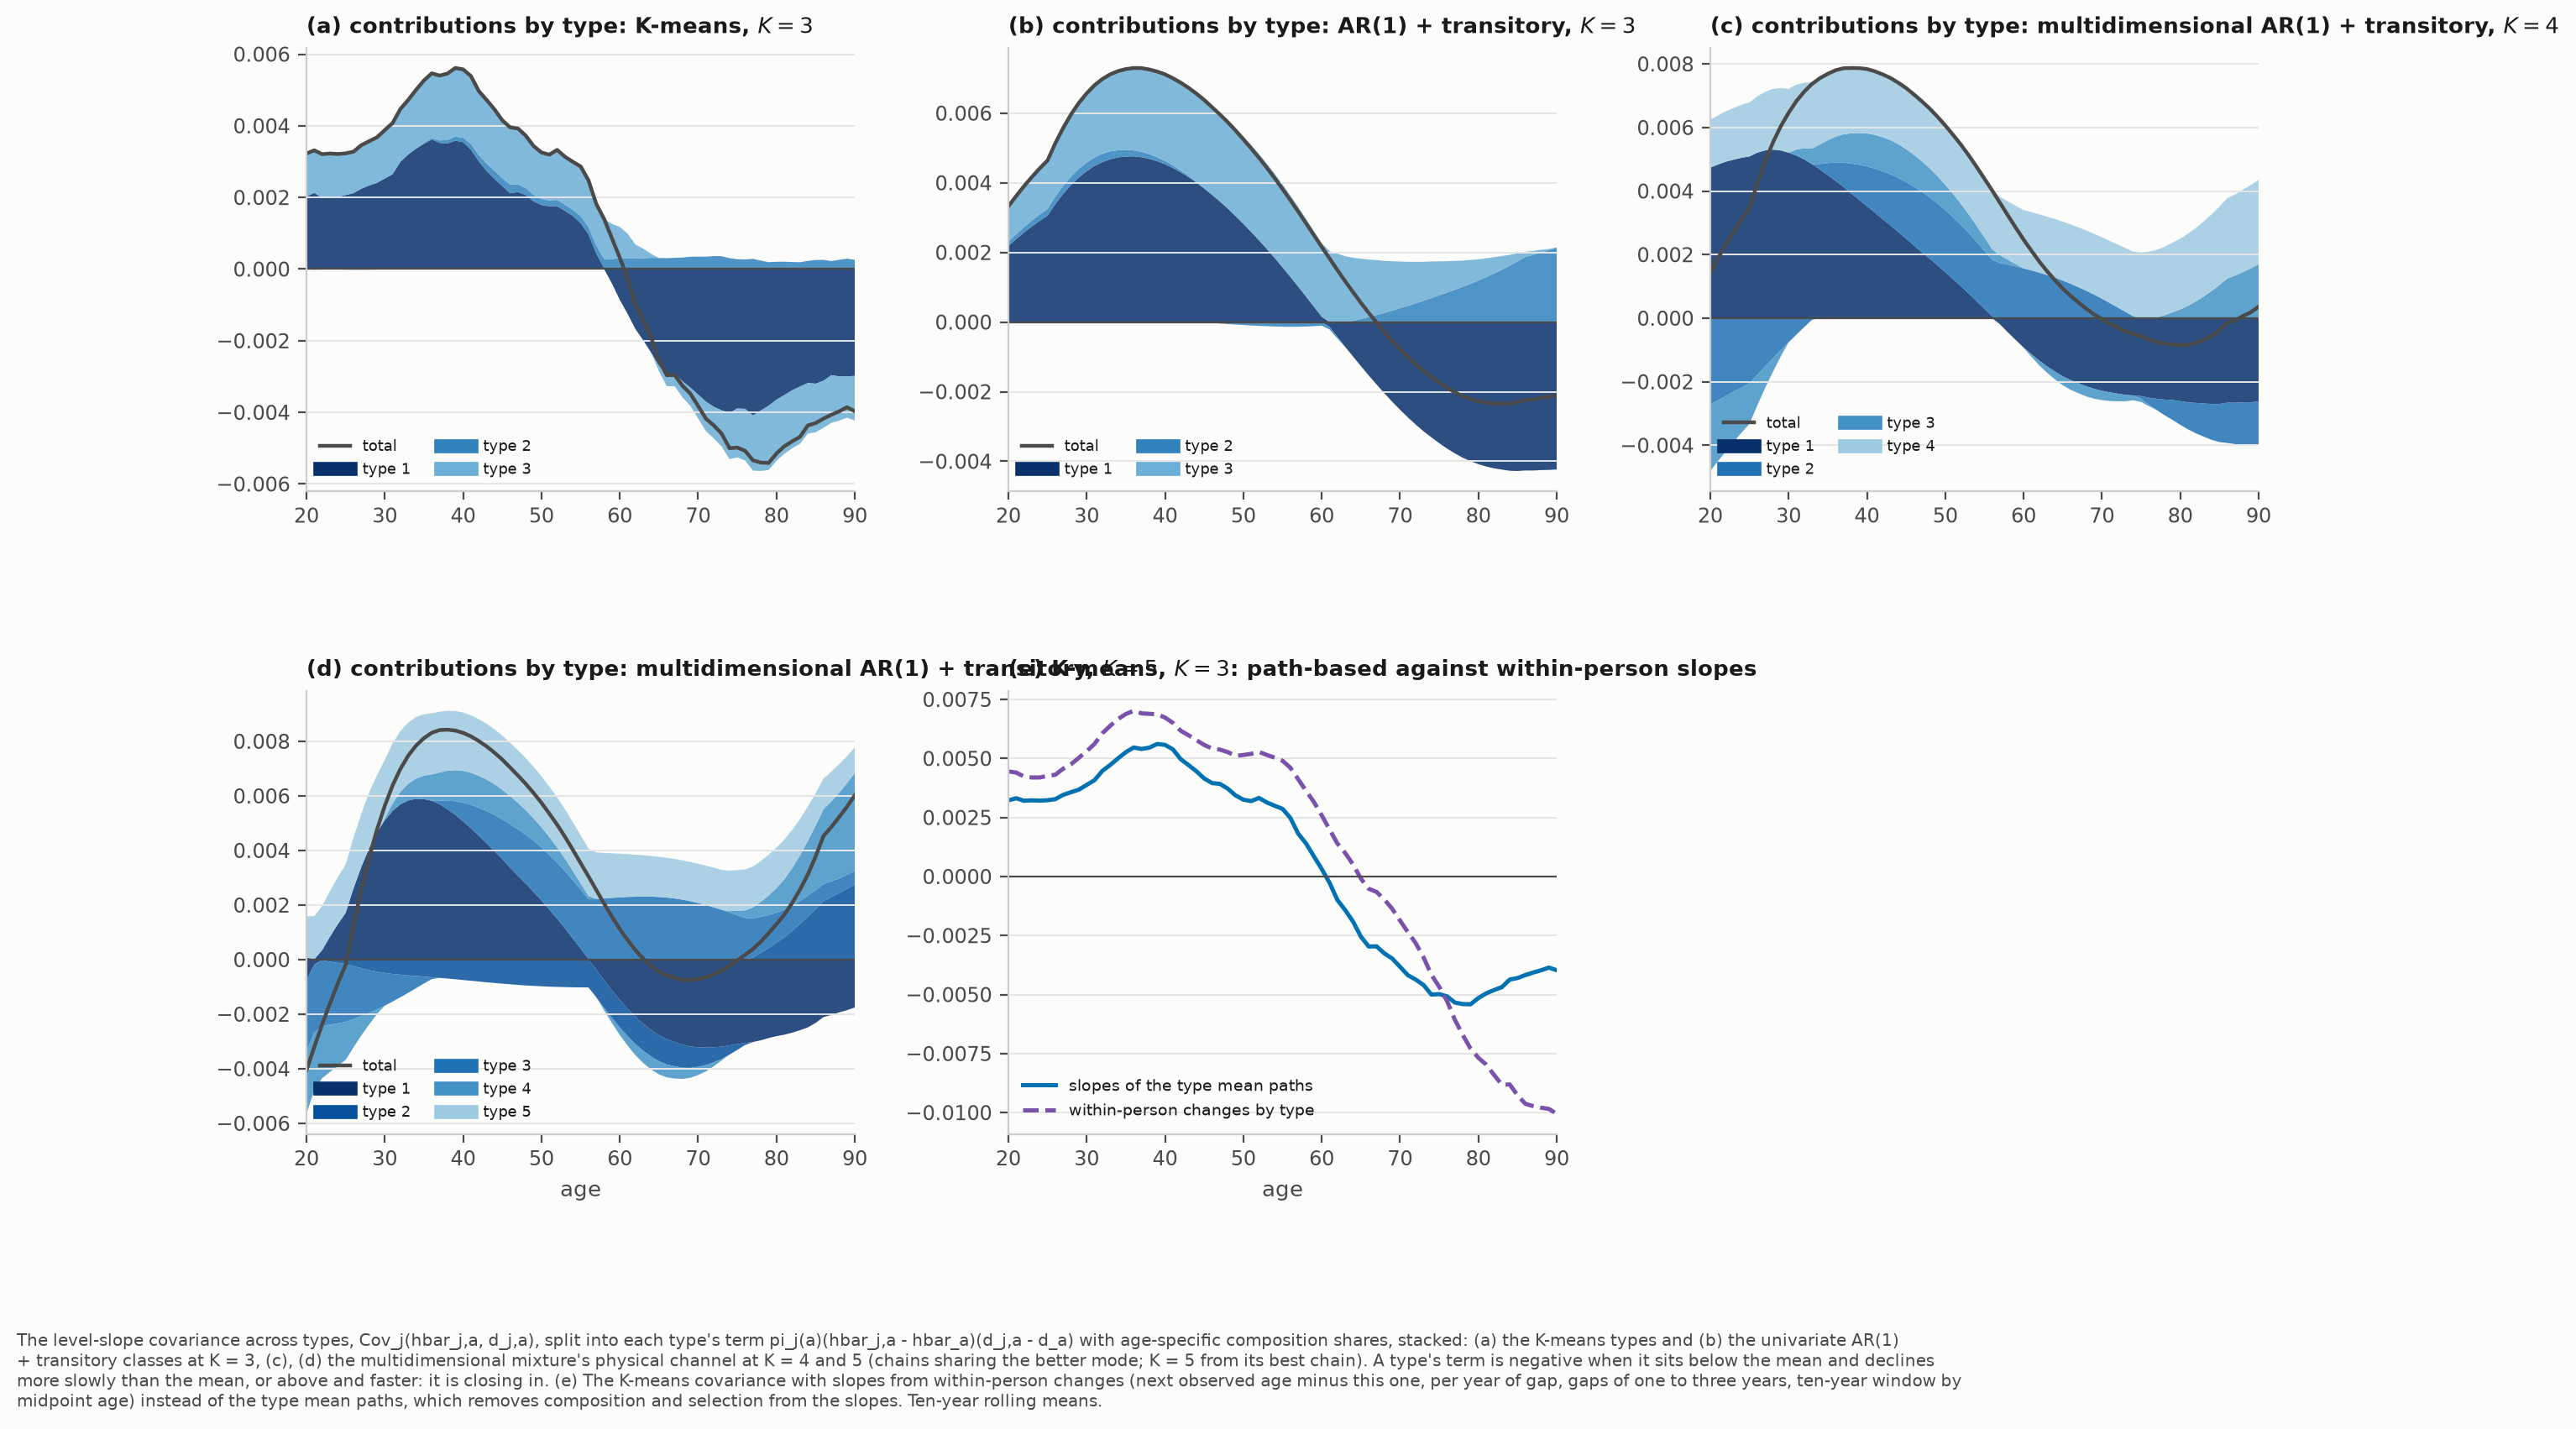
\includegraphics[width=\linewidth]{fig_reversal_types.png}
	\caption{The level--slope covariance split into each type's term, by typology.}
	\label{fig:reversaltypes}
\end{figure}

\subsection{Birth-Decade Cohort Effects}
\label{app:cohort}\label{app:kmeans_cohort}
\begin{itemize}
	\item Neither K-means with flexible age nor the mixtures with decade shifts change the typology; believe the flexible version's shifts (zero before 1970).
\end{itemize}
\begin{figure}[H]\centering
	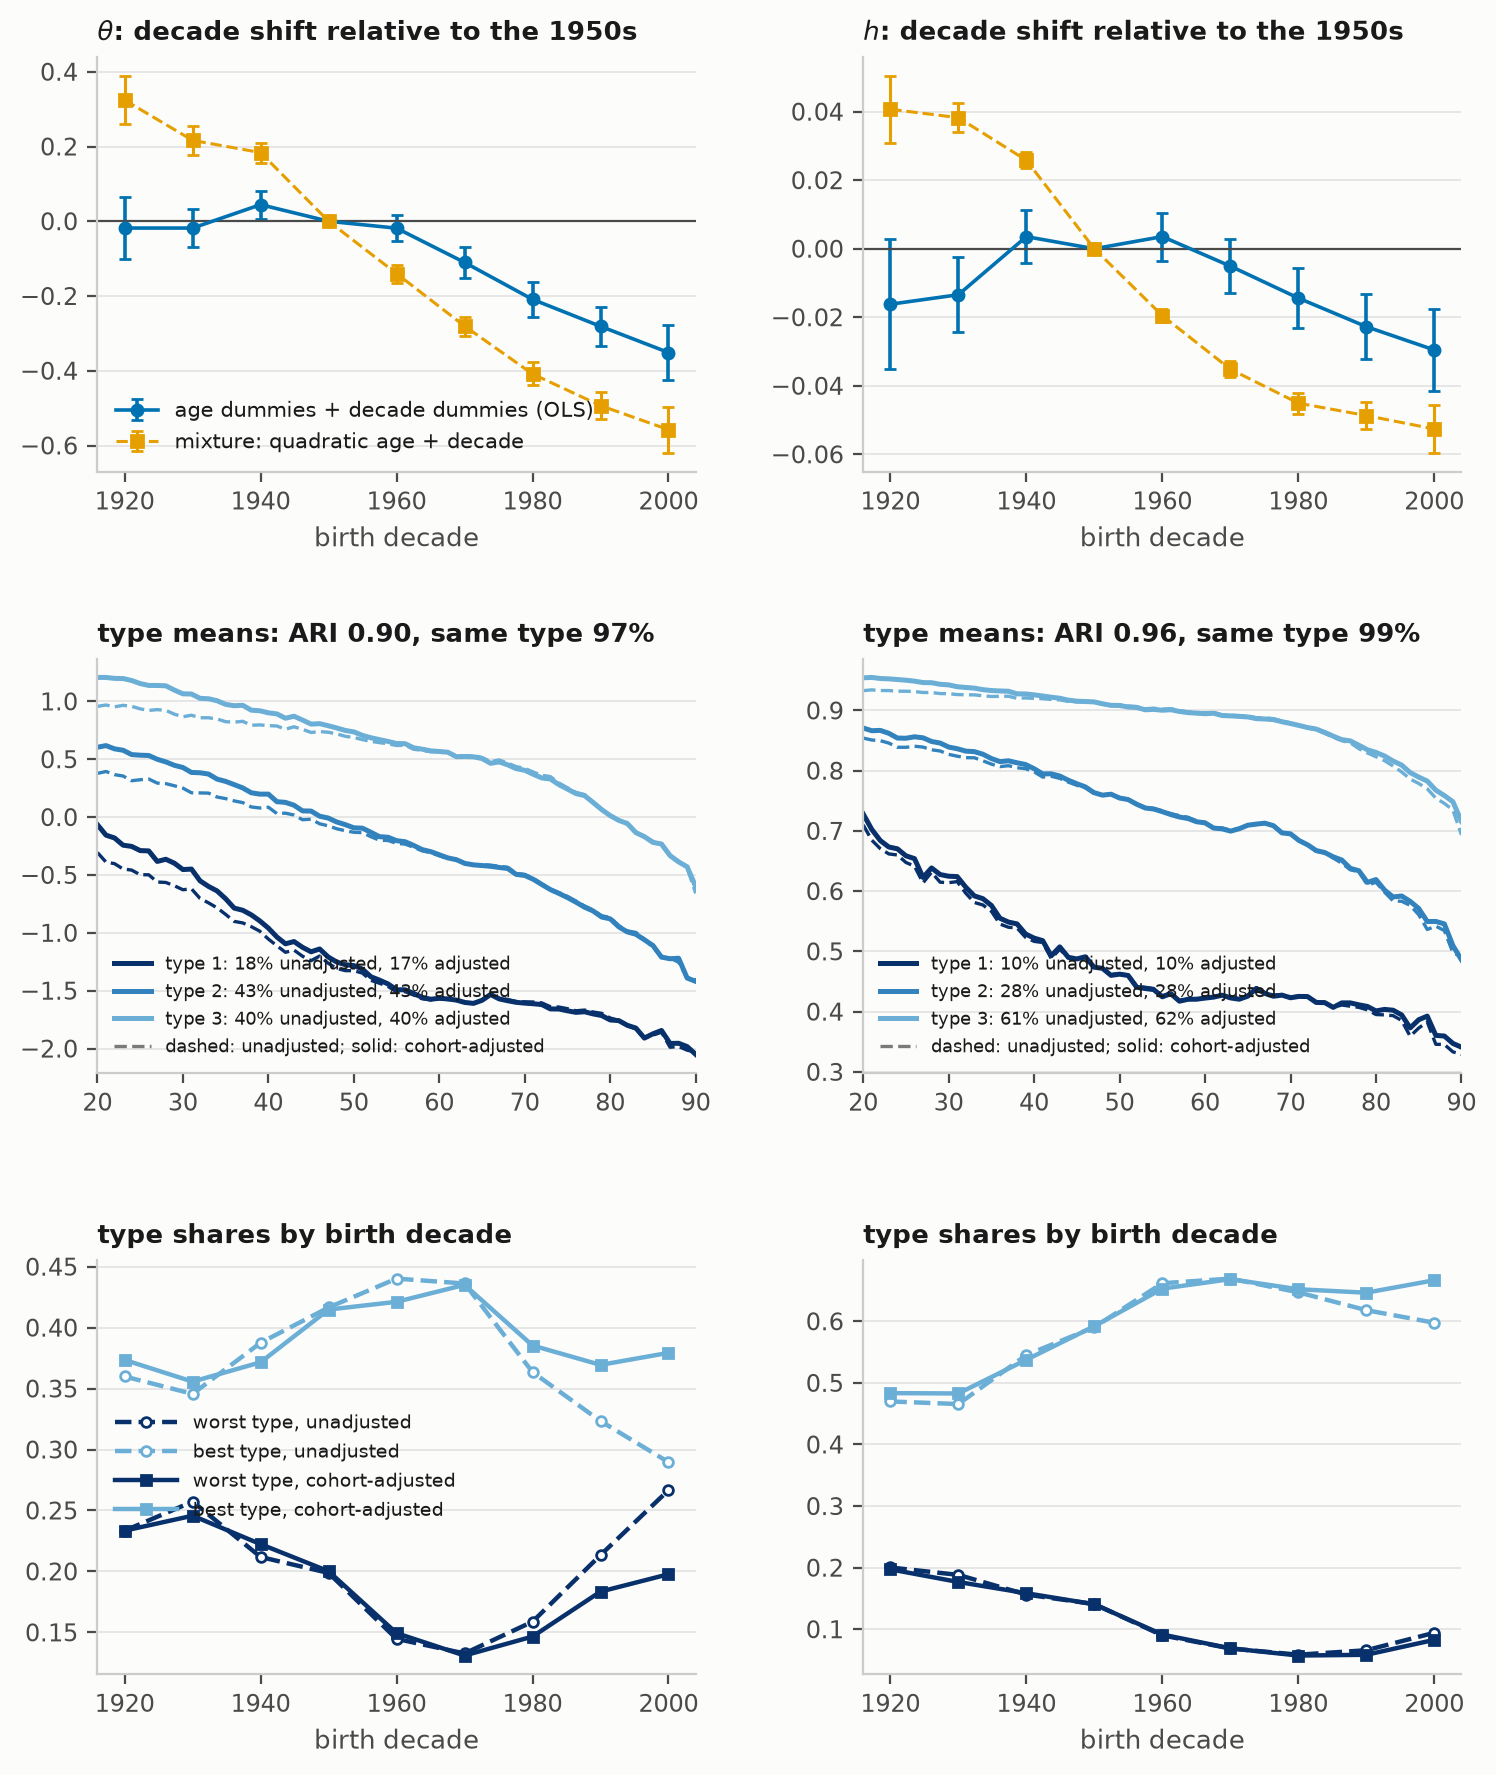
\includegraphics[width=0.75\linewidth]{fig_kmeans_cohort.png}
	\caption{Cohort adjustment within partial K-means.}
	\label{fig:kmeanscohort}
\end{figure}
\begin{figure}[H]\centering
	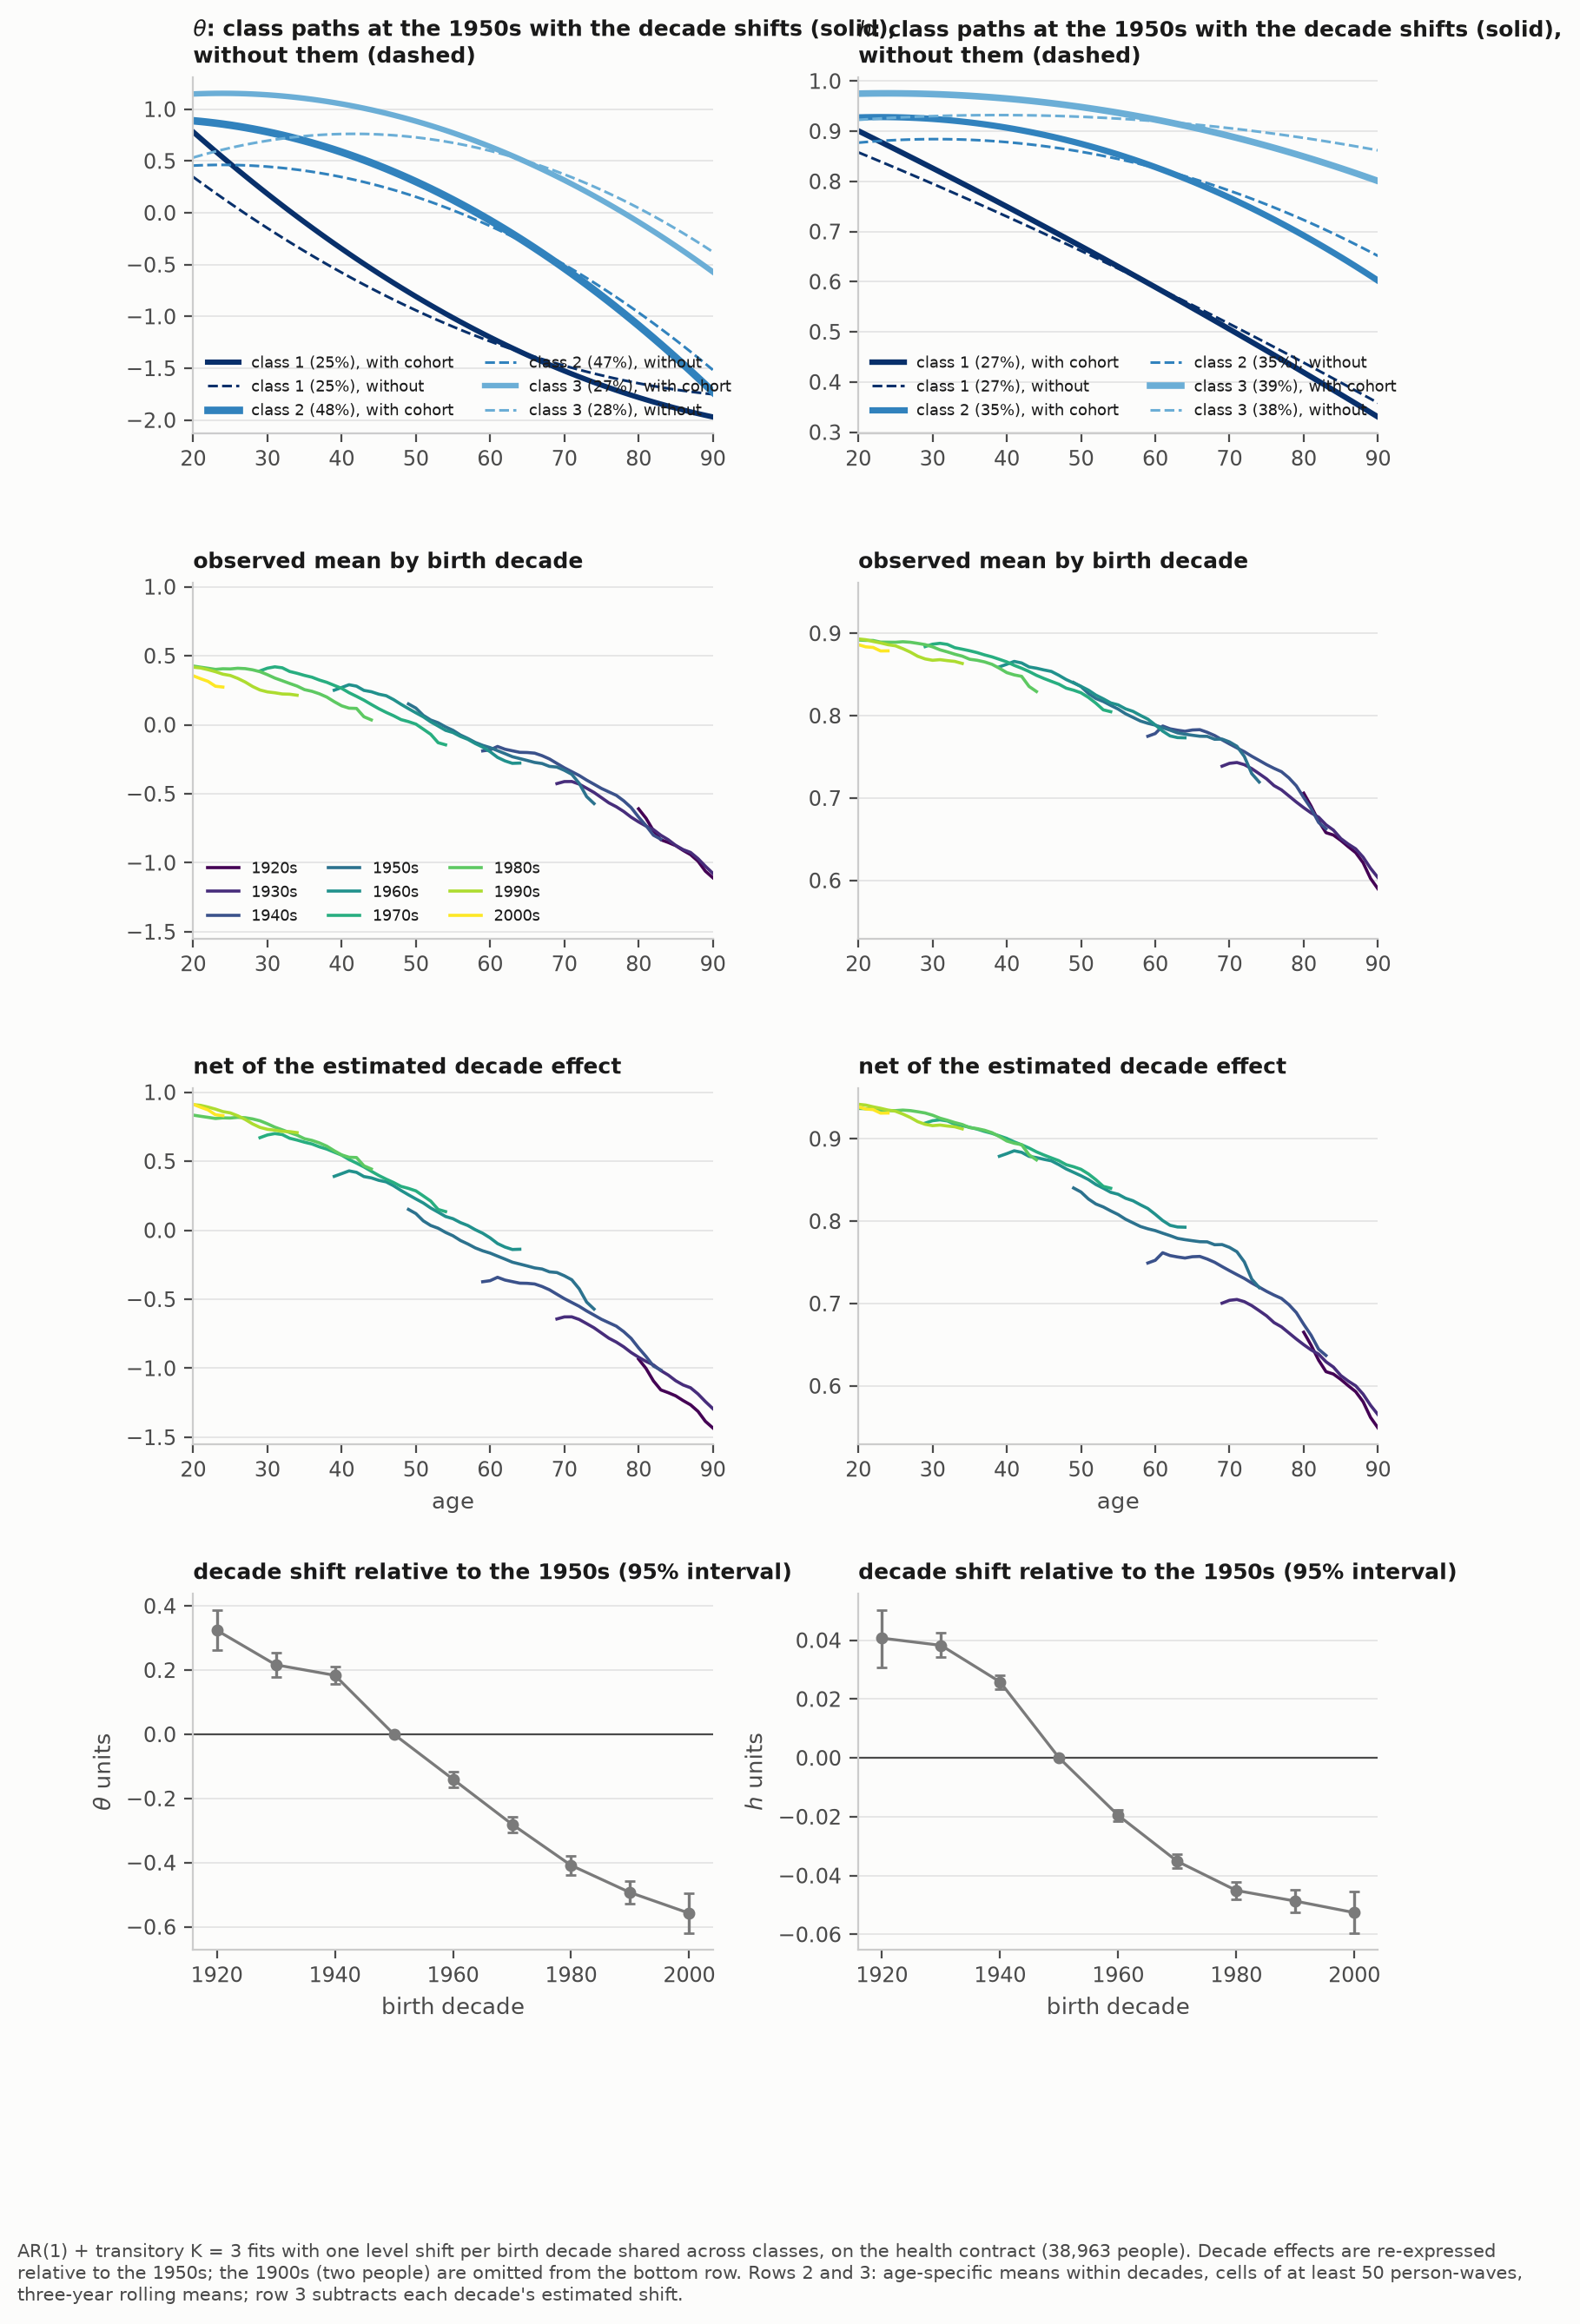
\includegraphics[width=0.62\linewidth]{fig_cohort.png}
	\caption{Single-channel mixtures with birth-decade shifts.}
	\label{fig:cohort}
\end{figure}
\begin{figure}[H]\centering
	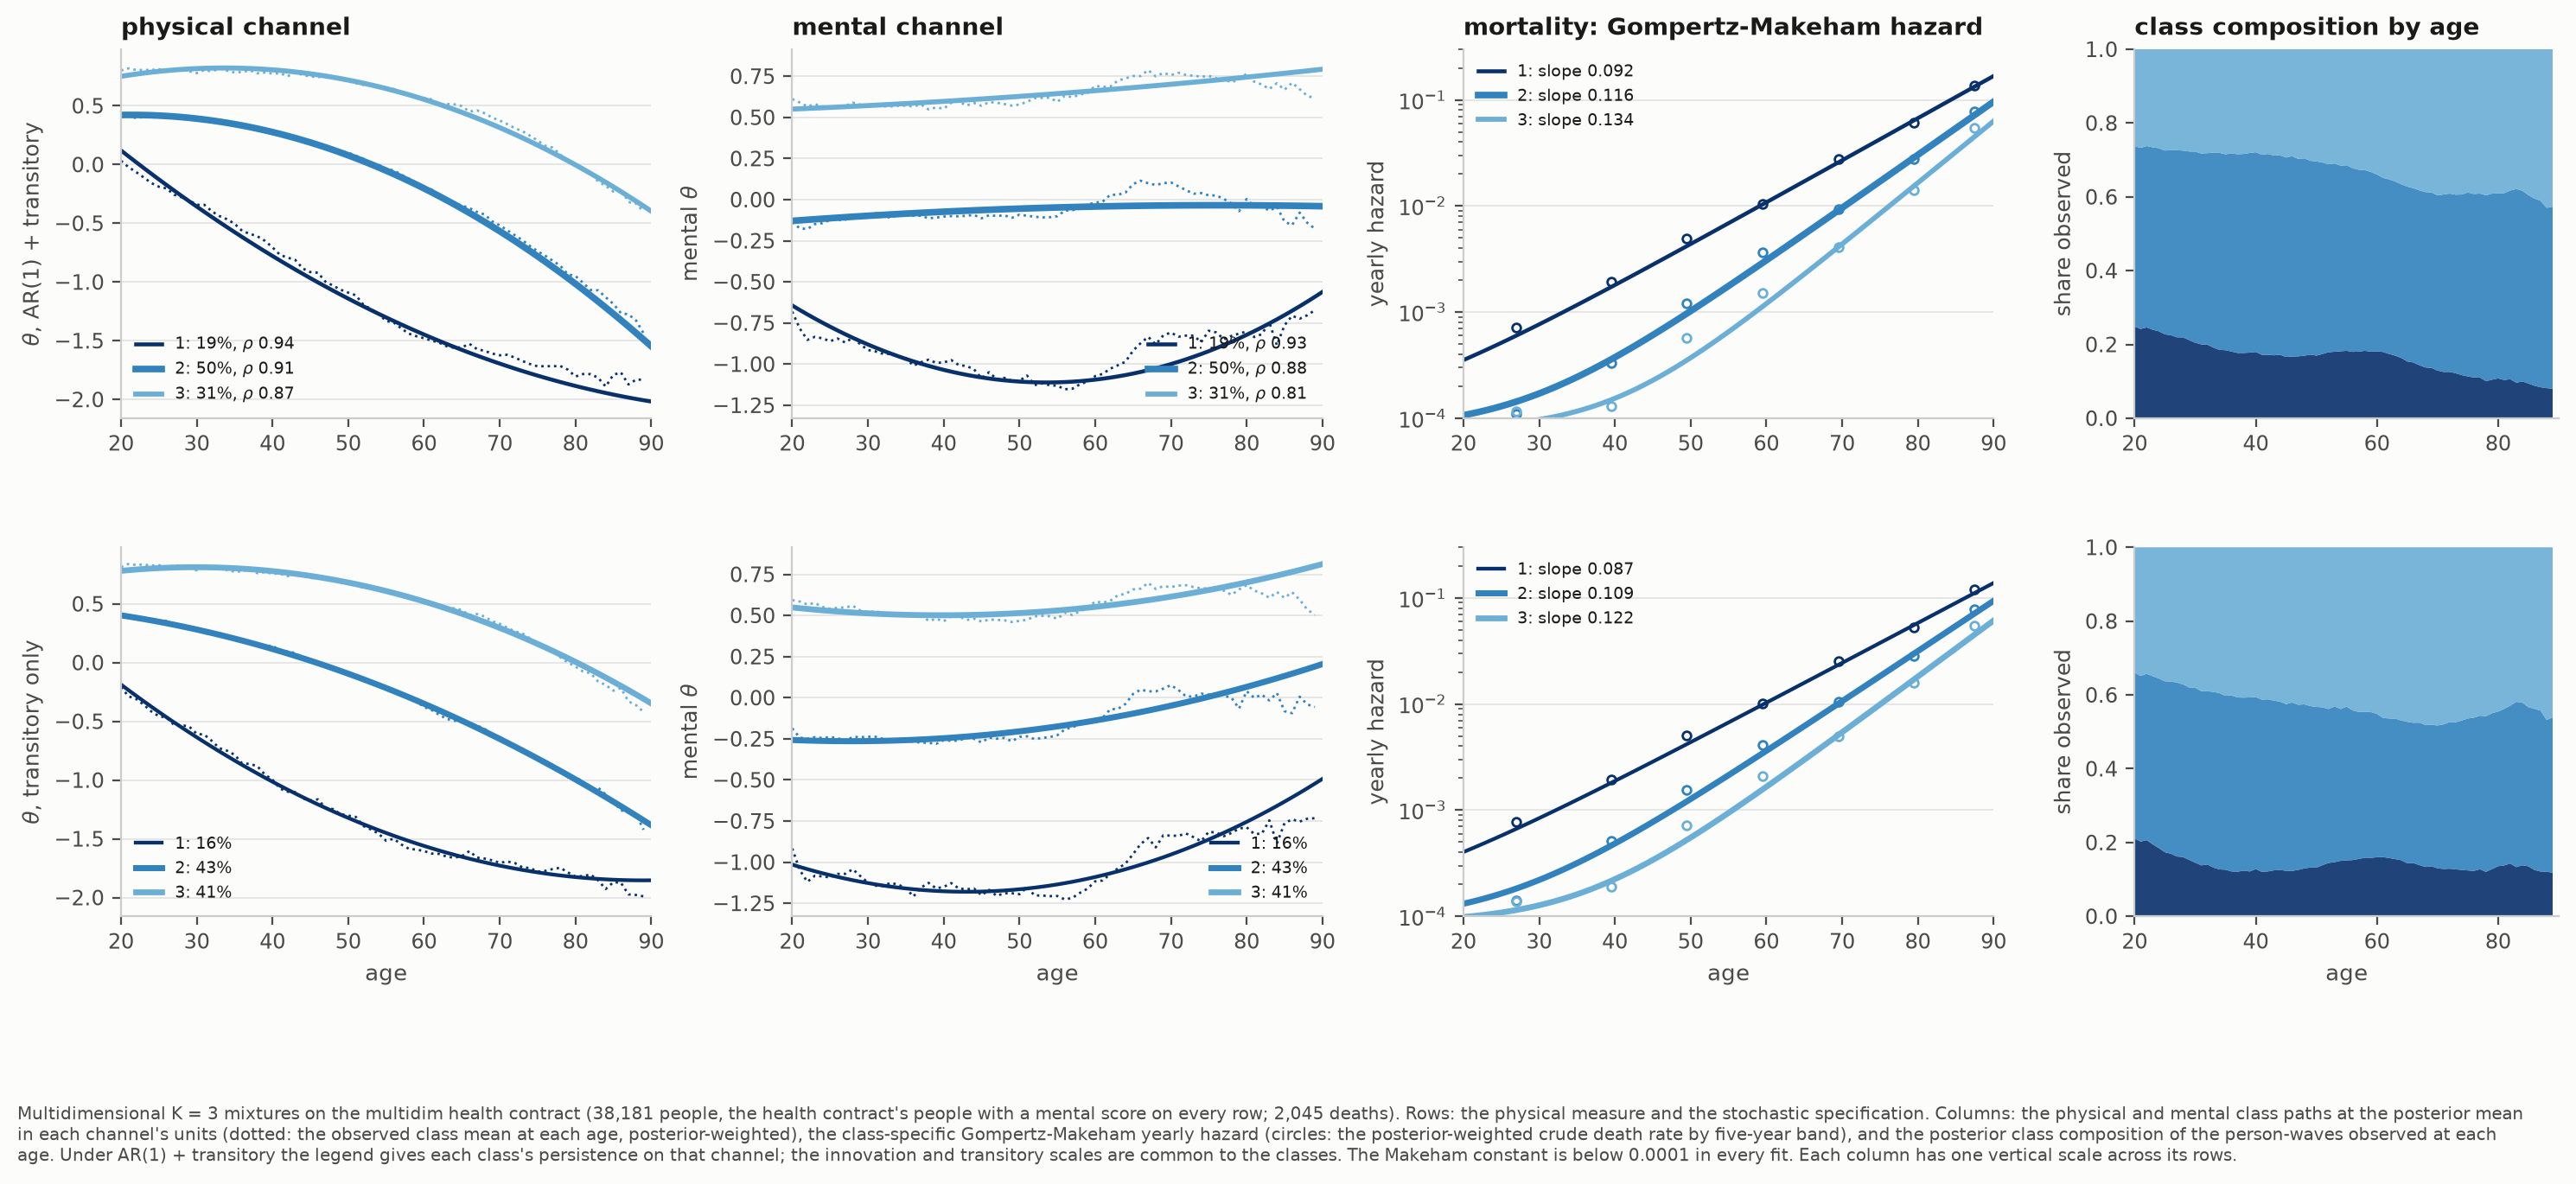
\includegraphics[width=\linewidth]{fig_multidim_trajectories.png}
	\caption{Multidimensional $K=3$ mixtures without the decade shifts.}
	\label{fig:multidim_nocohort}
\end{figure}
\begin{figure}[H]\centering
	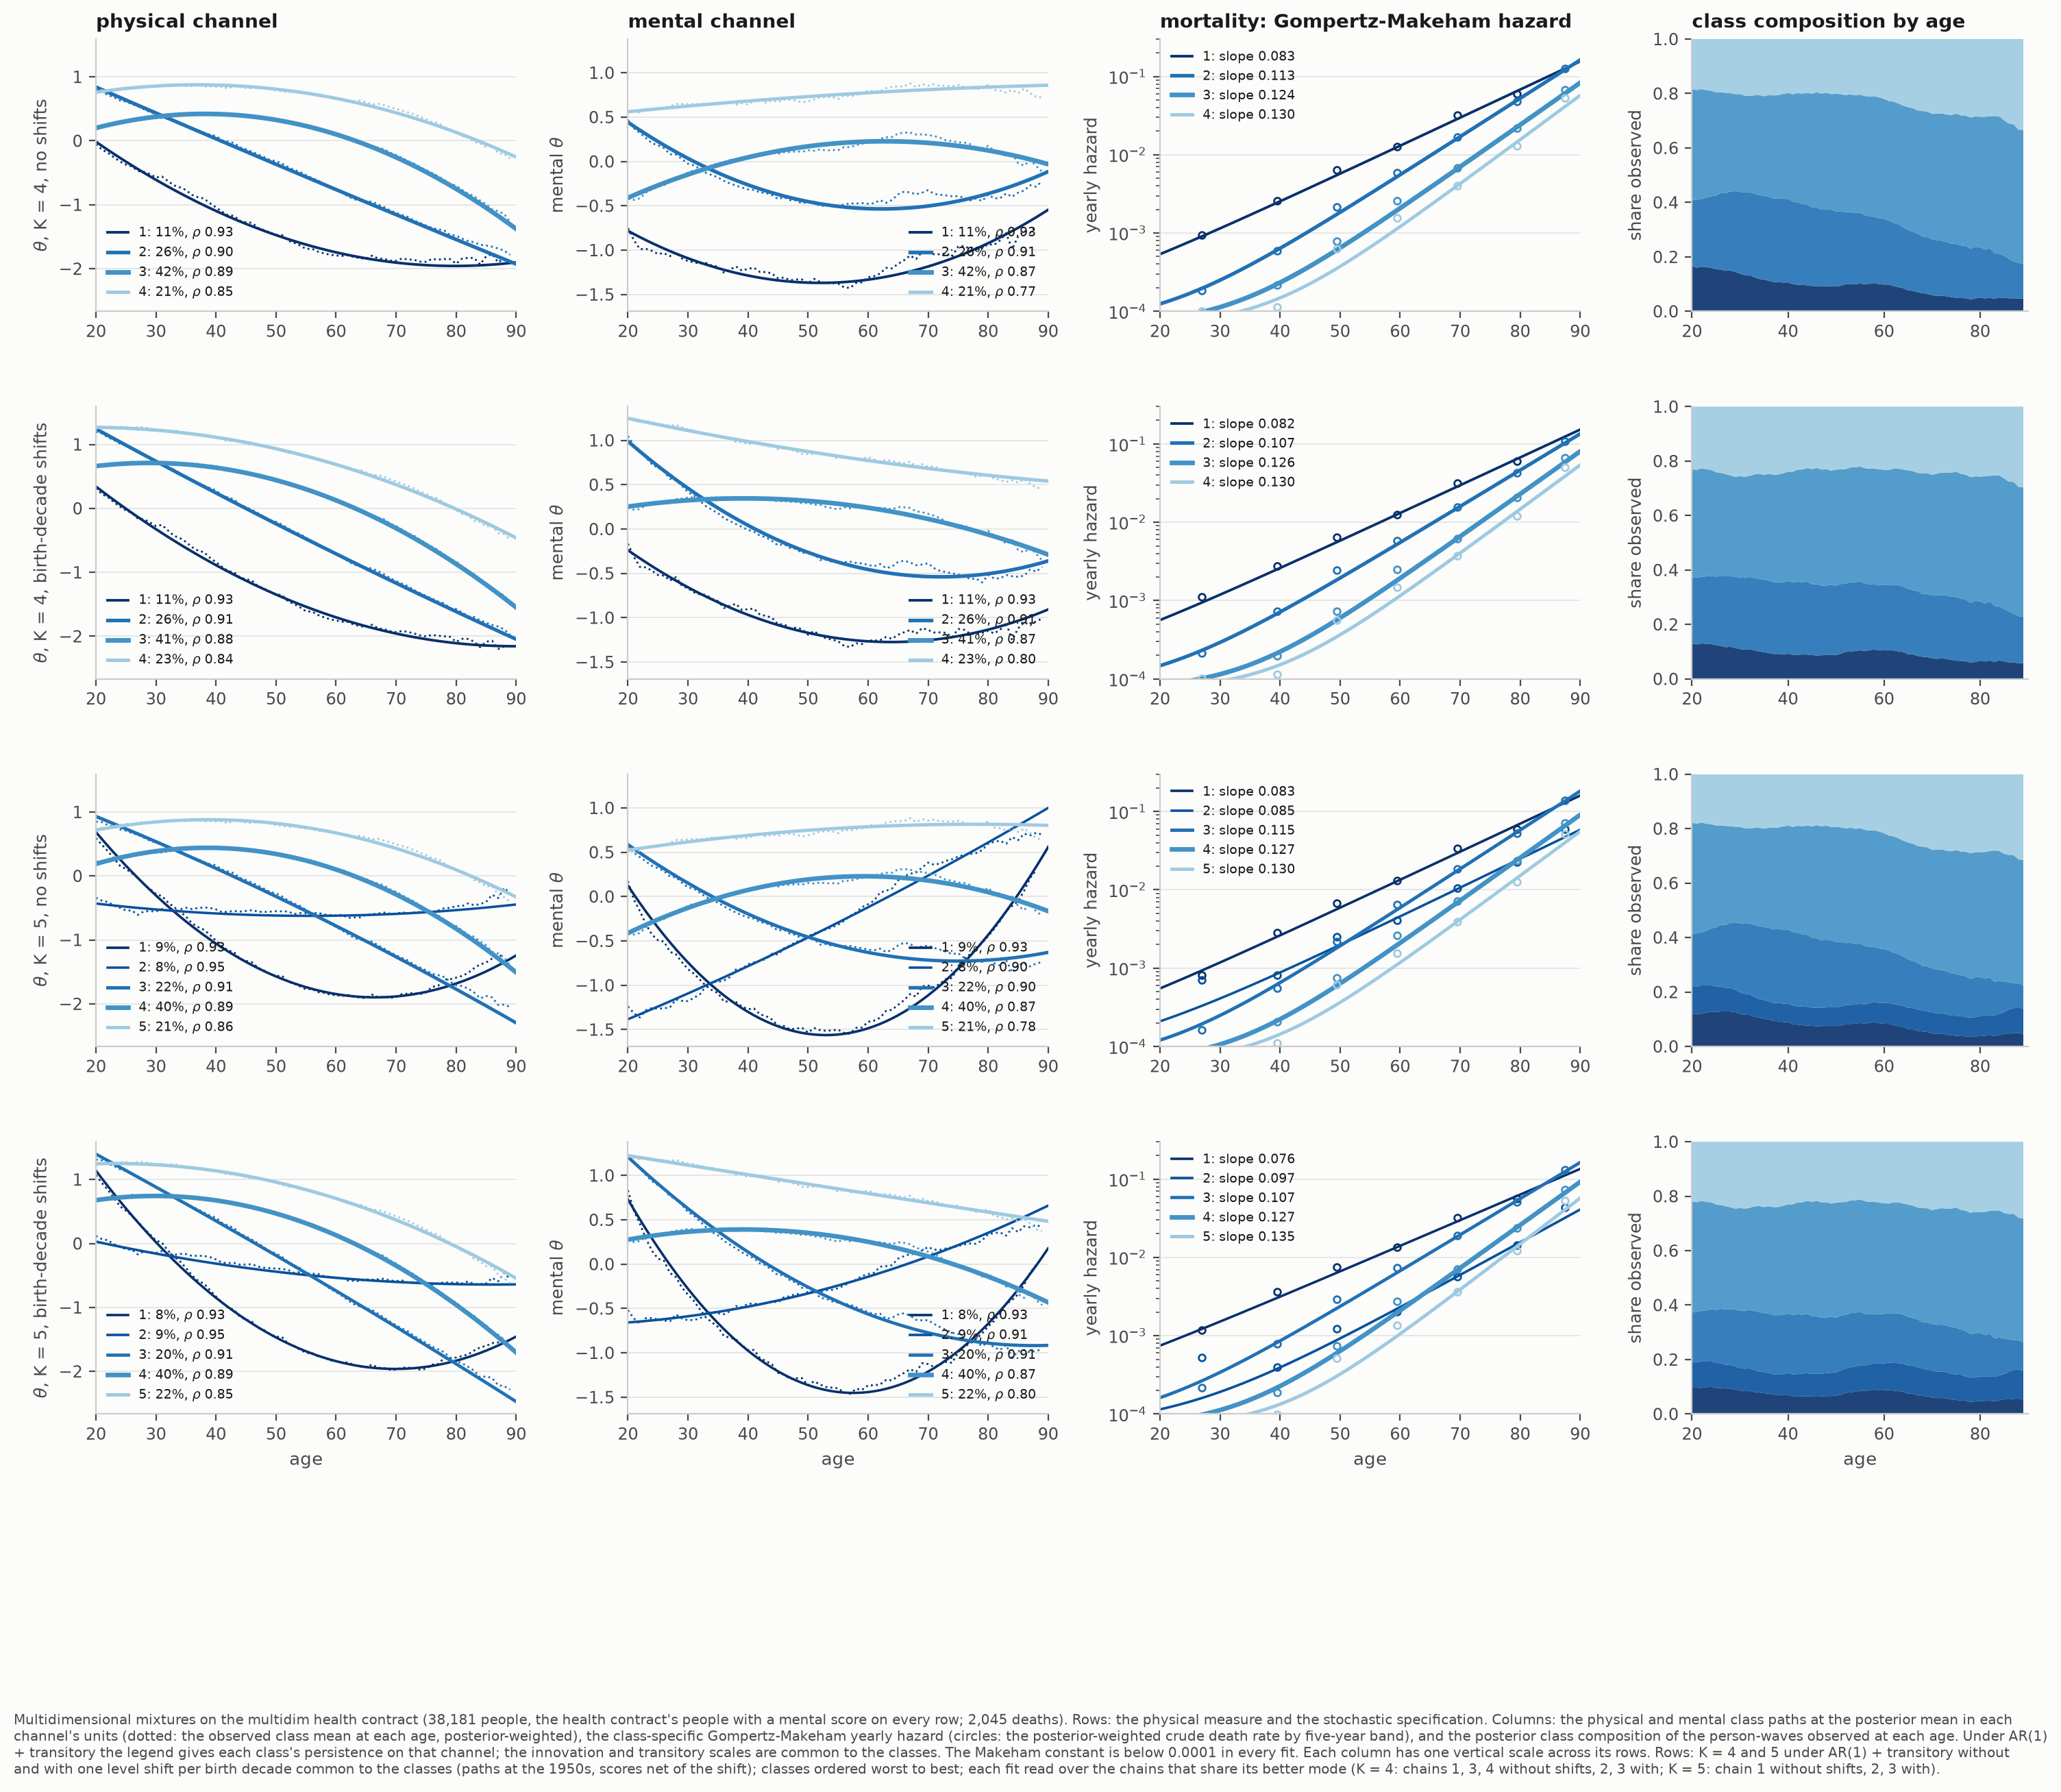
\includegraphics[width=\linewidth]{fig_multidim_trajectories_by_K_cohort.png}
	\caption{Multidimensional $K=4$ and $K=5$ fits with and without decade shifts.}
	\label{fig:multidim_k4_cohort}
\end{figure}

\subsection{Multidimensional against Univariate Classes}
\label{app:multidim_vs_uni}
\begin{itemize}
	\item The multidimensional classes are the physical classes with a mental path attached; the mental score alone gives a different partition.
\end{itemize}
\begin{figure}[H]\centering
	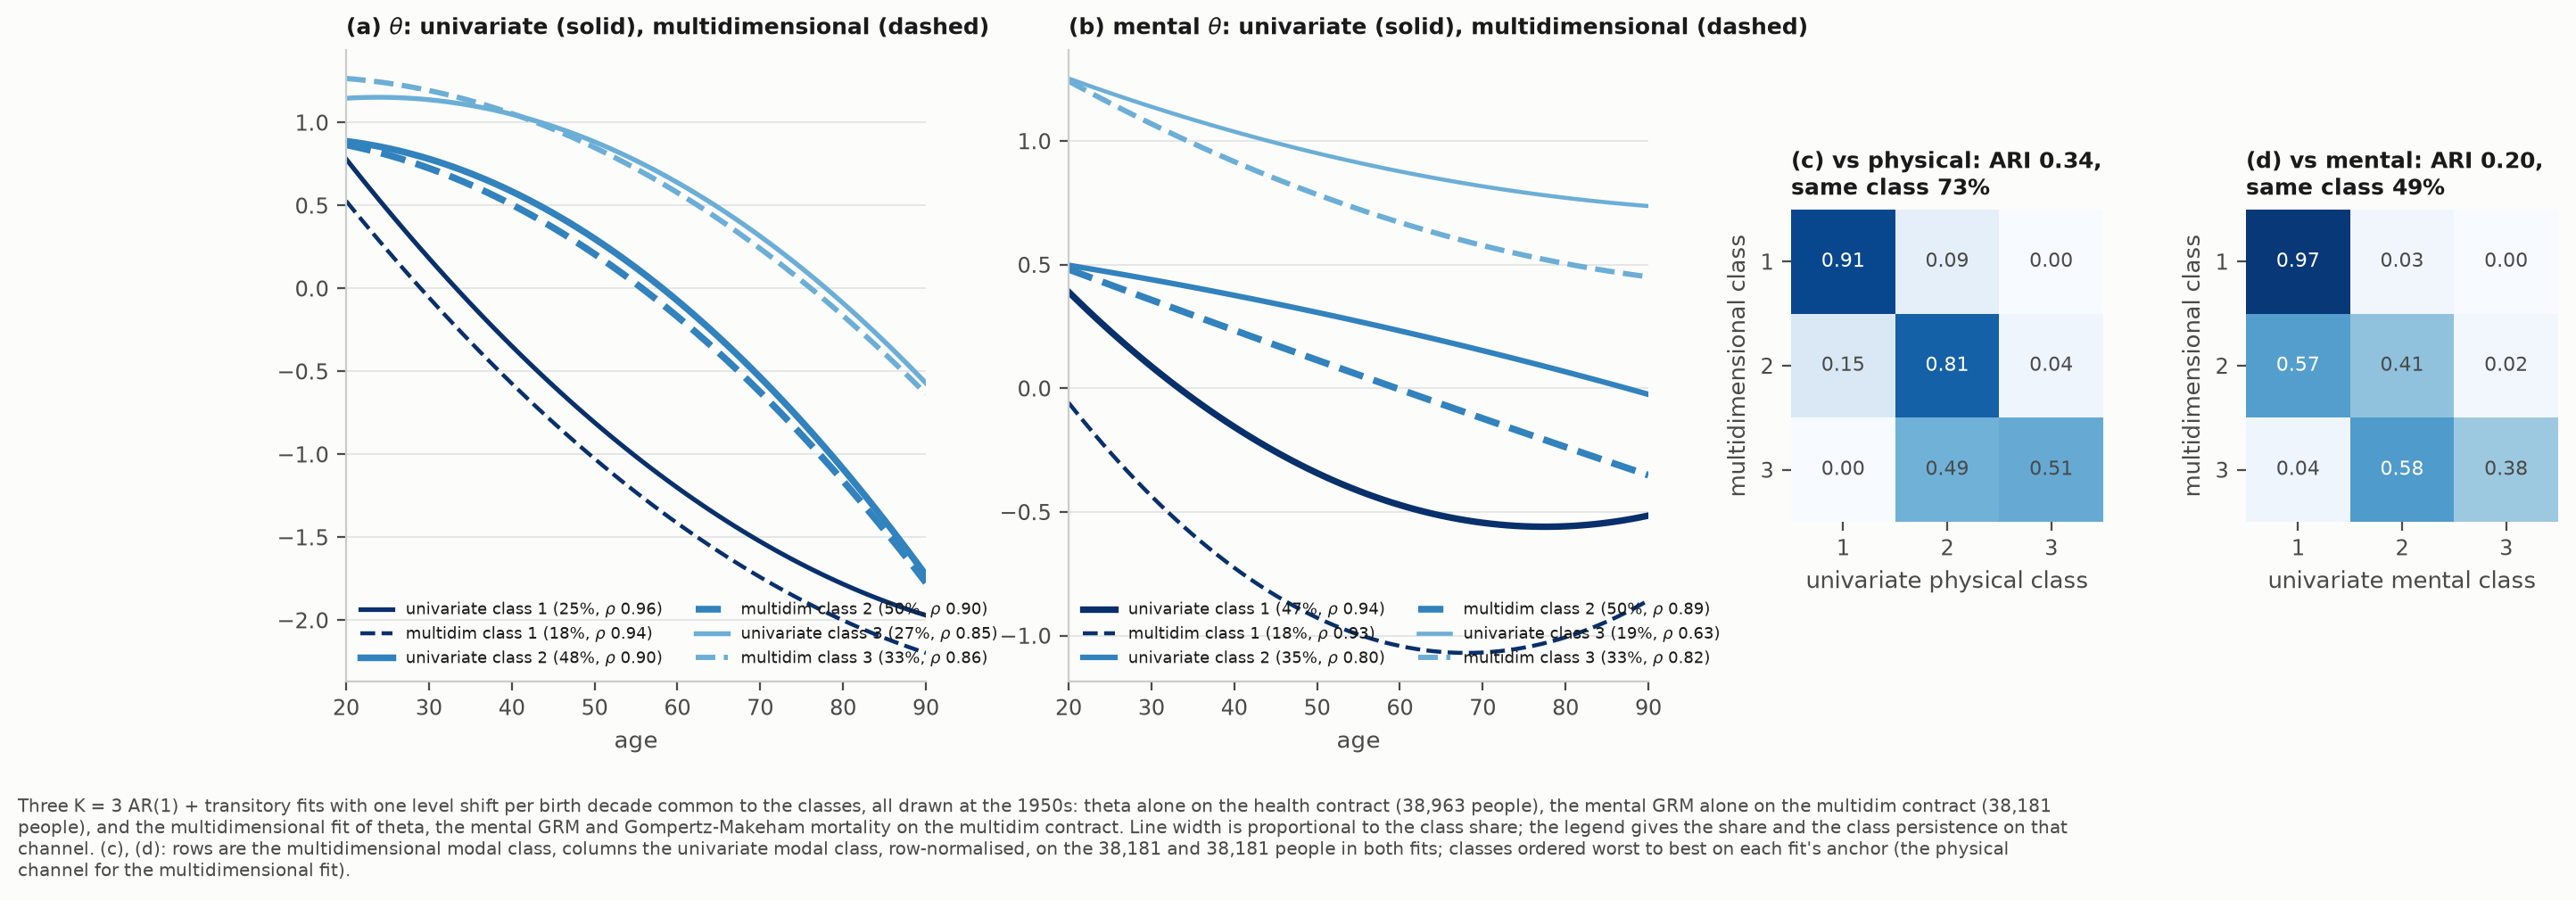
\includegraphics[width=\linewidth]{fig_multidim_vs_univariate.png}
	\caption{Multidimensional against univariate physical and mental classes.}
	\label{fig:multidim_vs_uni}
\end{figure}

\subsection{The Windows at Four Classes}
\label{app:windows_k4}
\begin{figure}[H]\centering
	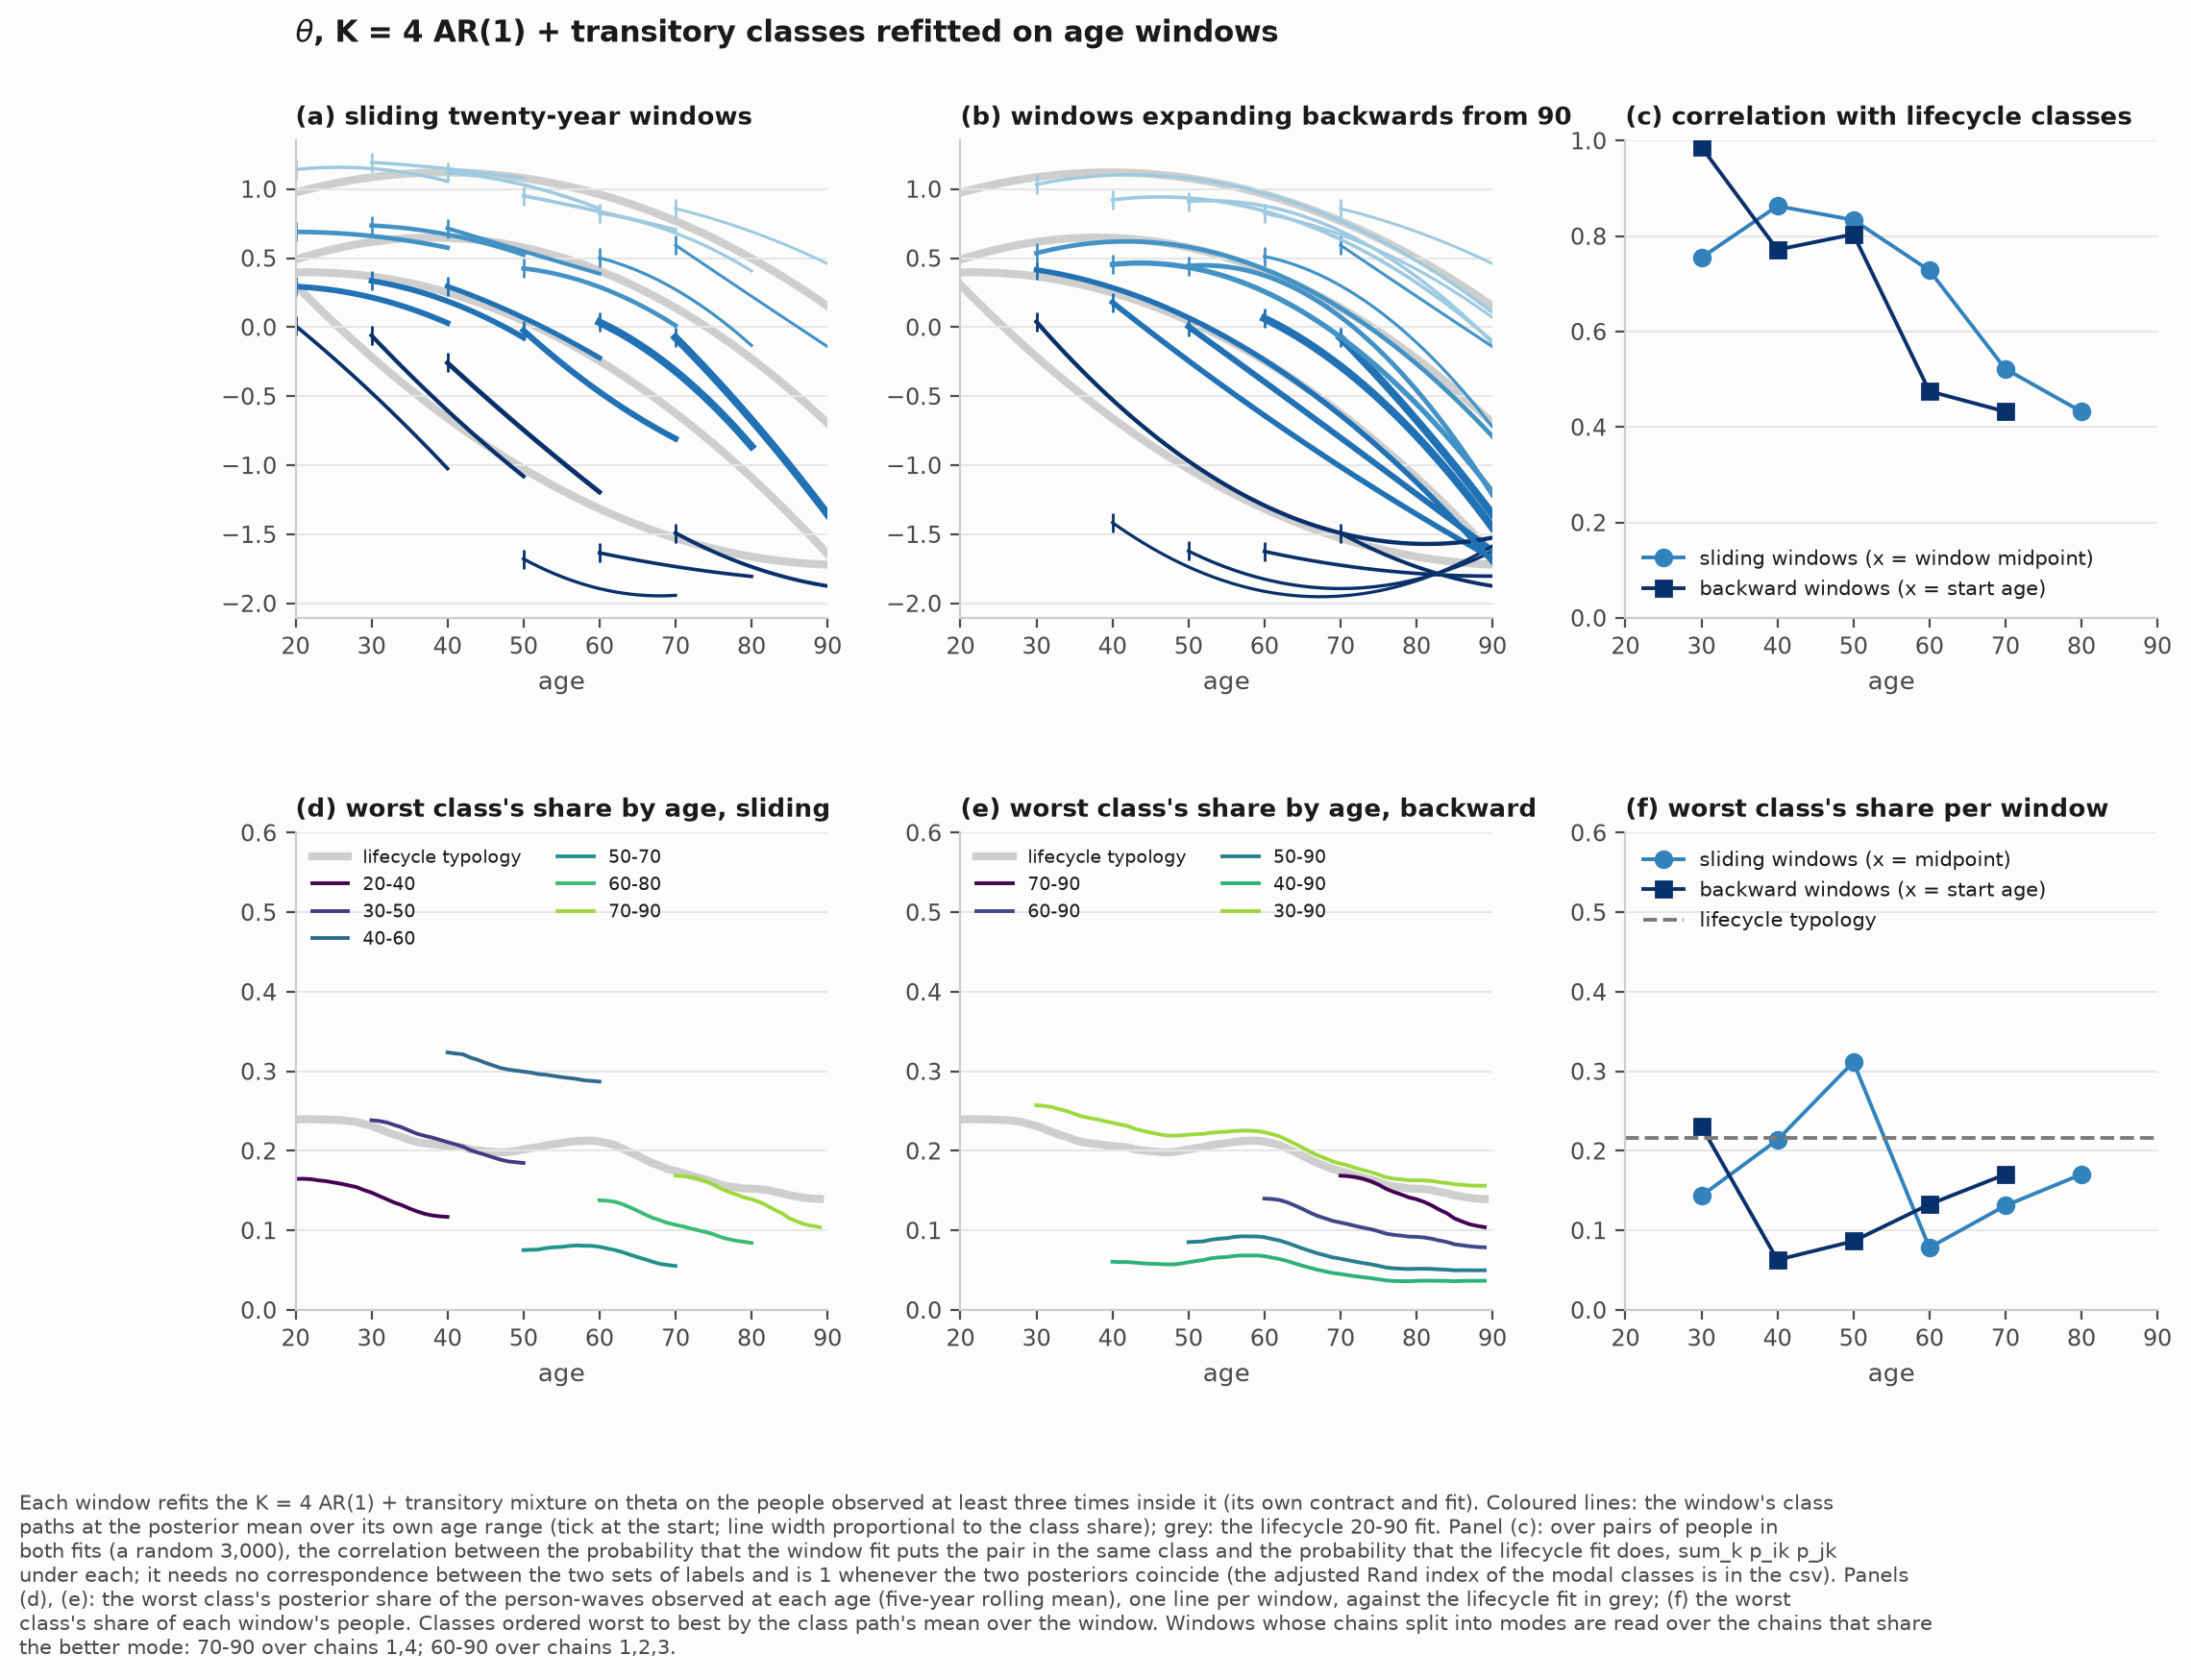
\includegraphics[width=\linewidth]{fig_windows_bayes_k4.png}
	\caption{As Figure~\ref{fig:windows}, at $K=4$.}
	\label{fig:windows_k4}
\end{figure}

\subsection{Predicting Death}
\label{app:predmort}
\begin{figure}[H]\centering
	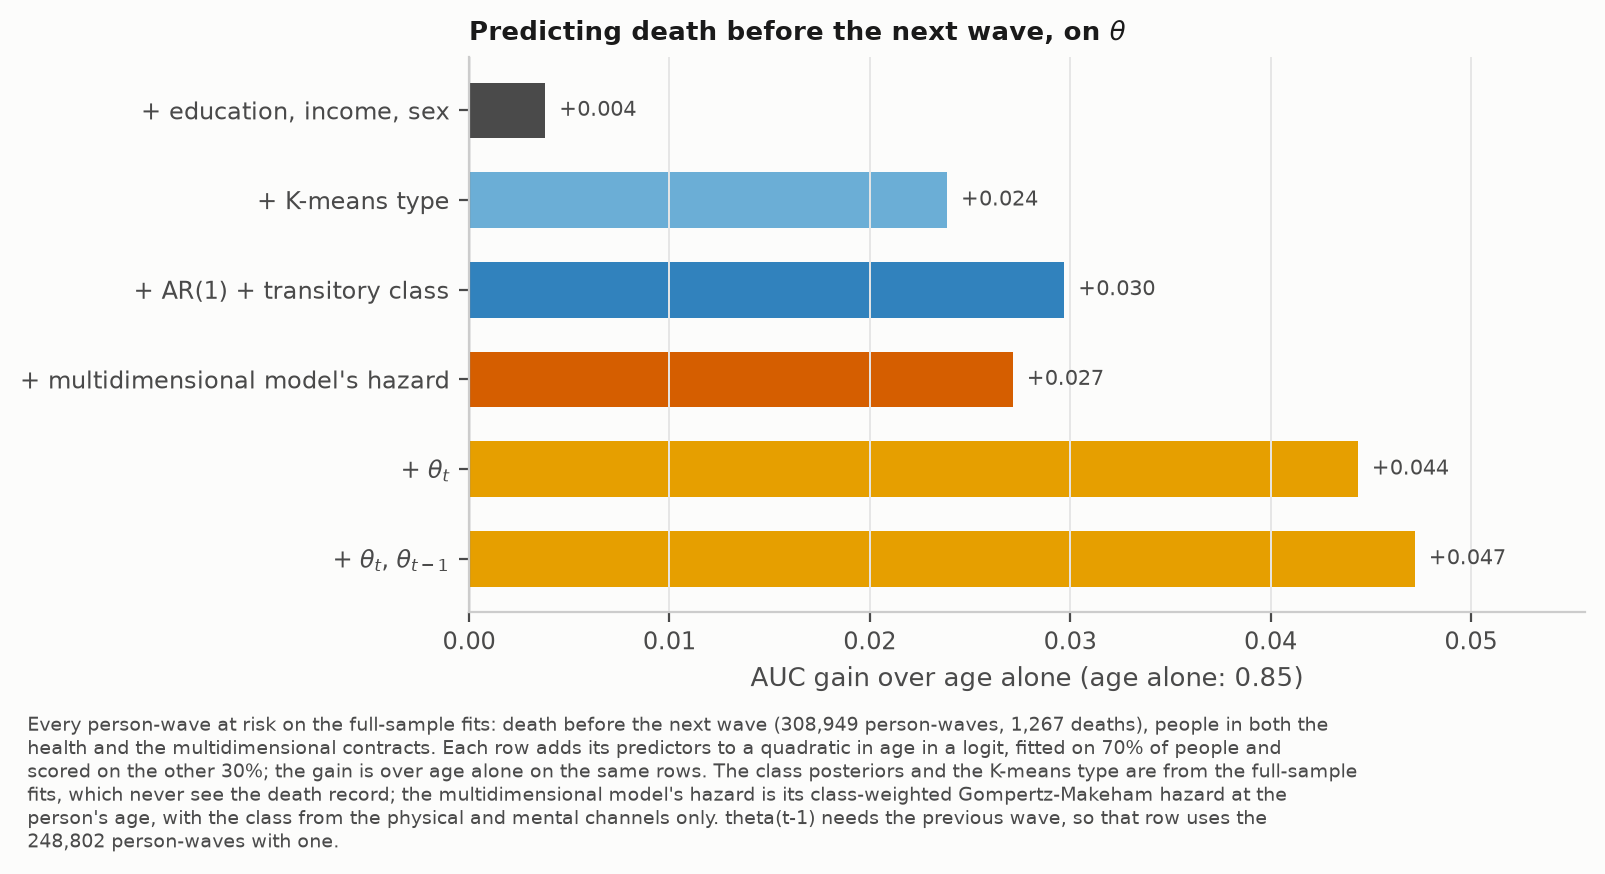
\includegraphics[width=0.75\linewidth]{fig_prediction_mortality_slim.png}
	\caption{AUC gain over age in predicting death before the next wave, on $\theta$.}
	\label{fig:predmort}
\end{figure}

\section{Additional Results on the Returns to Prevention}
\label{app:returns}

\subsection{The Estimated Cost Curve}
\label{app:costcurve}
\begin{itemize}
	\item Close to age-invariant below 75; the 75--90 band sits 32\% above, so late-life cost is understated.
\end{itemize}
\begin{figure}[H]\centering
	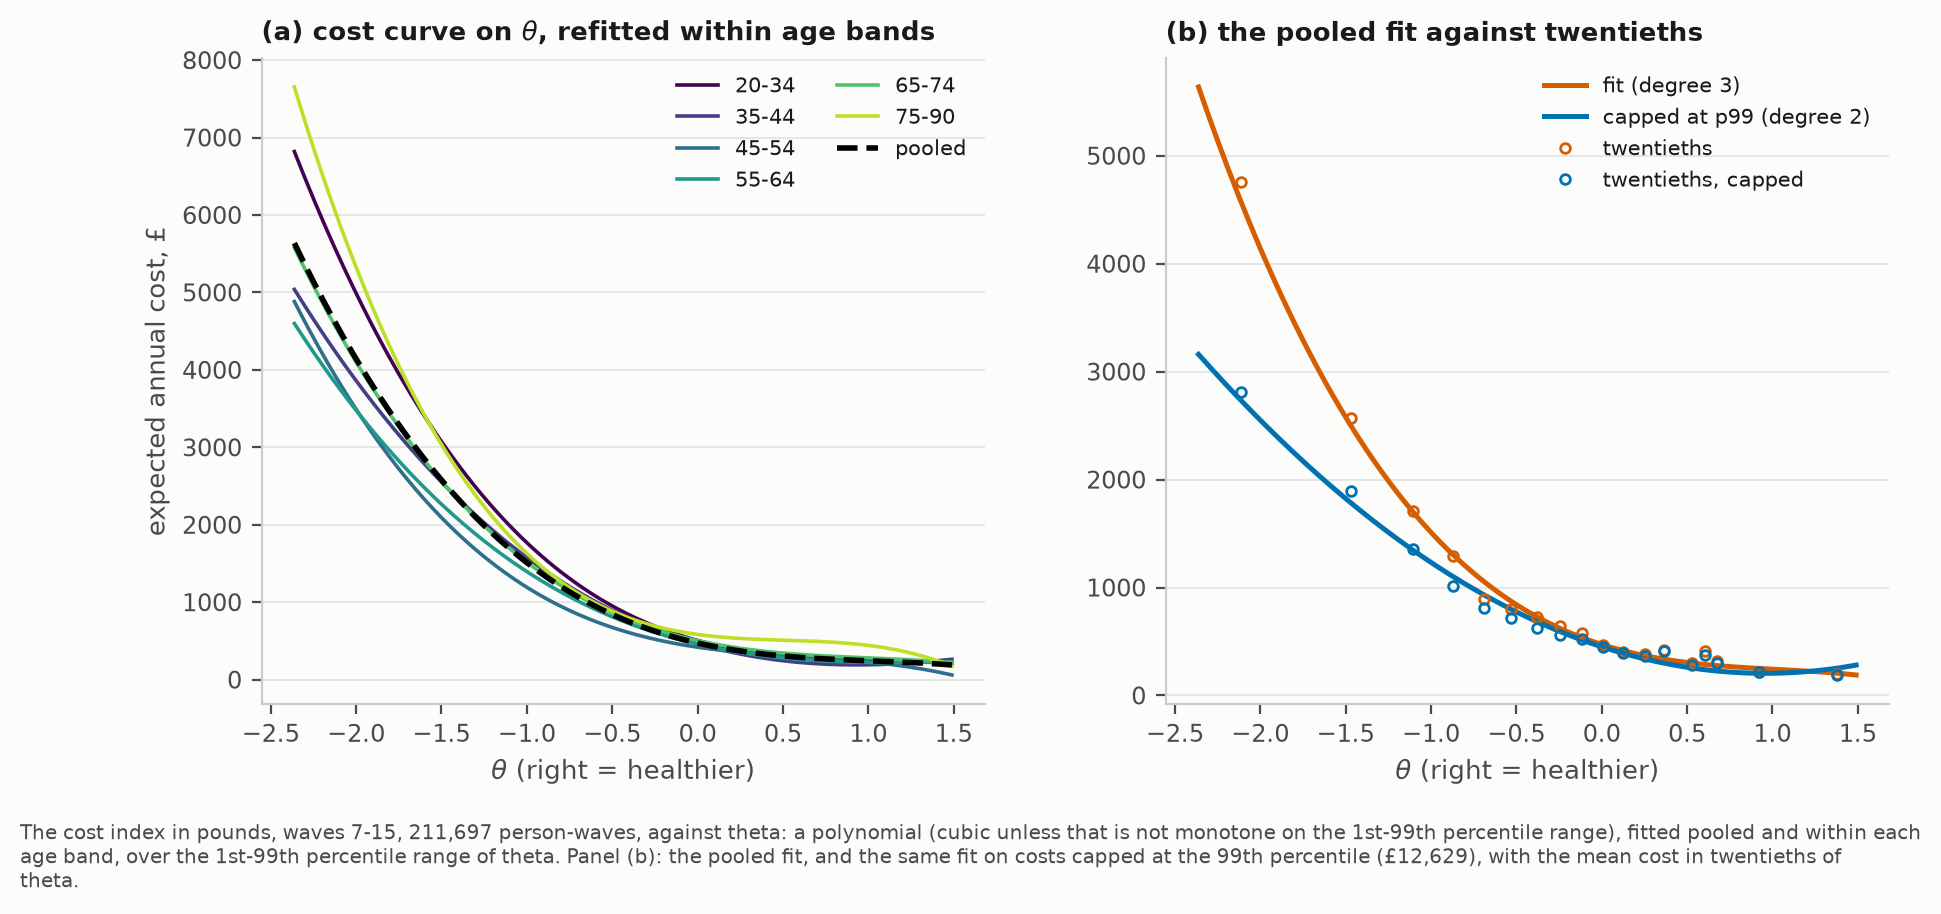
\includegraphics[width=\linewidth]{fig_cost_curve.png}
	\caption{The cubic cost curve: by age band (a) and capped vs uncapped (b).}
	\label{fig:costcurve}
\end{figure}

\subsection{The Detailed Returns and the Targeting Rules}
\label{app:returns_detail}
\begin{figure}[H]\centering
	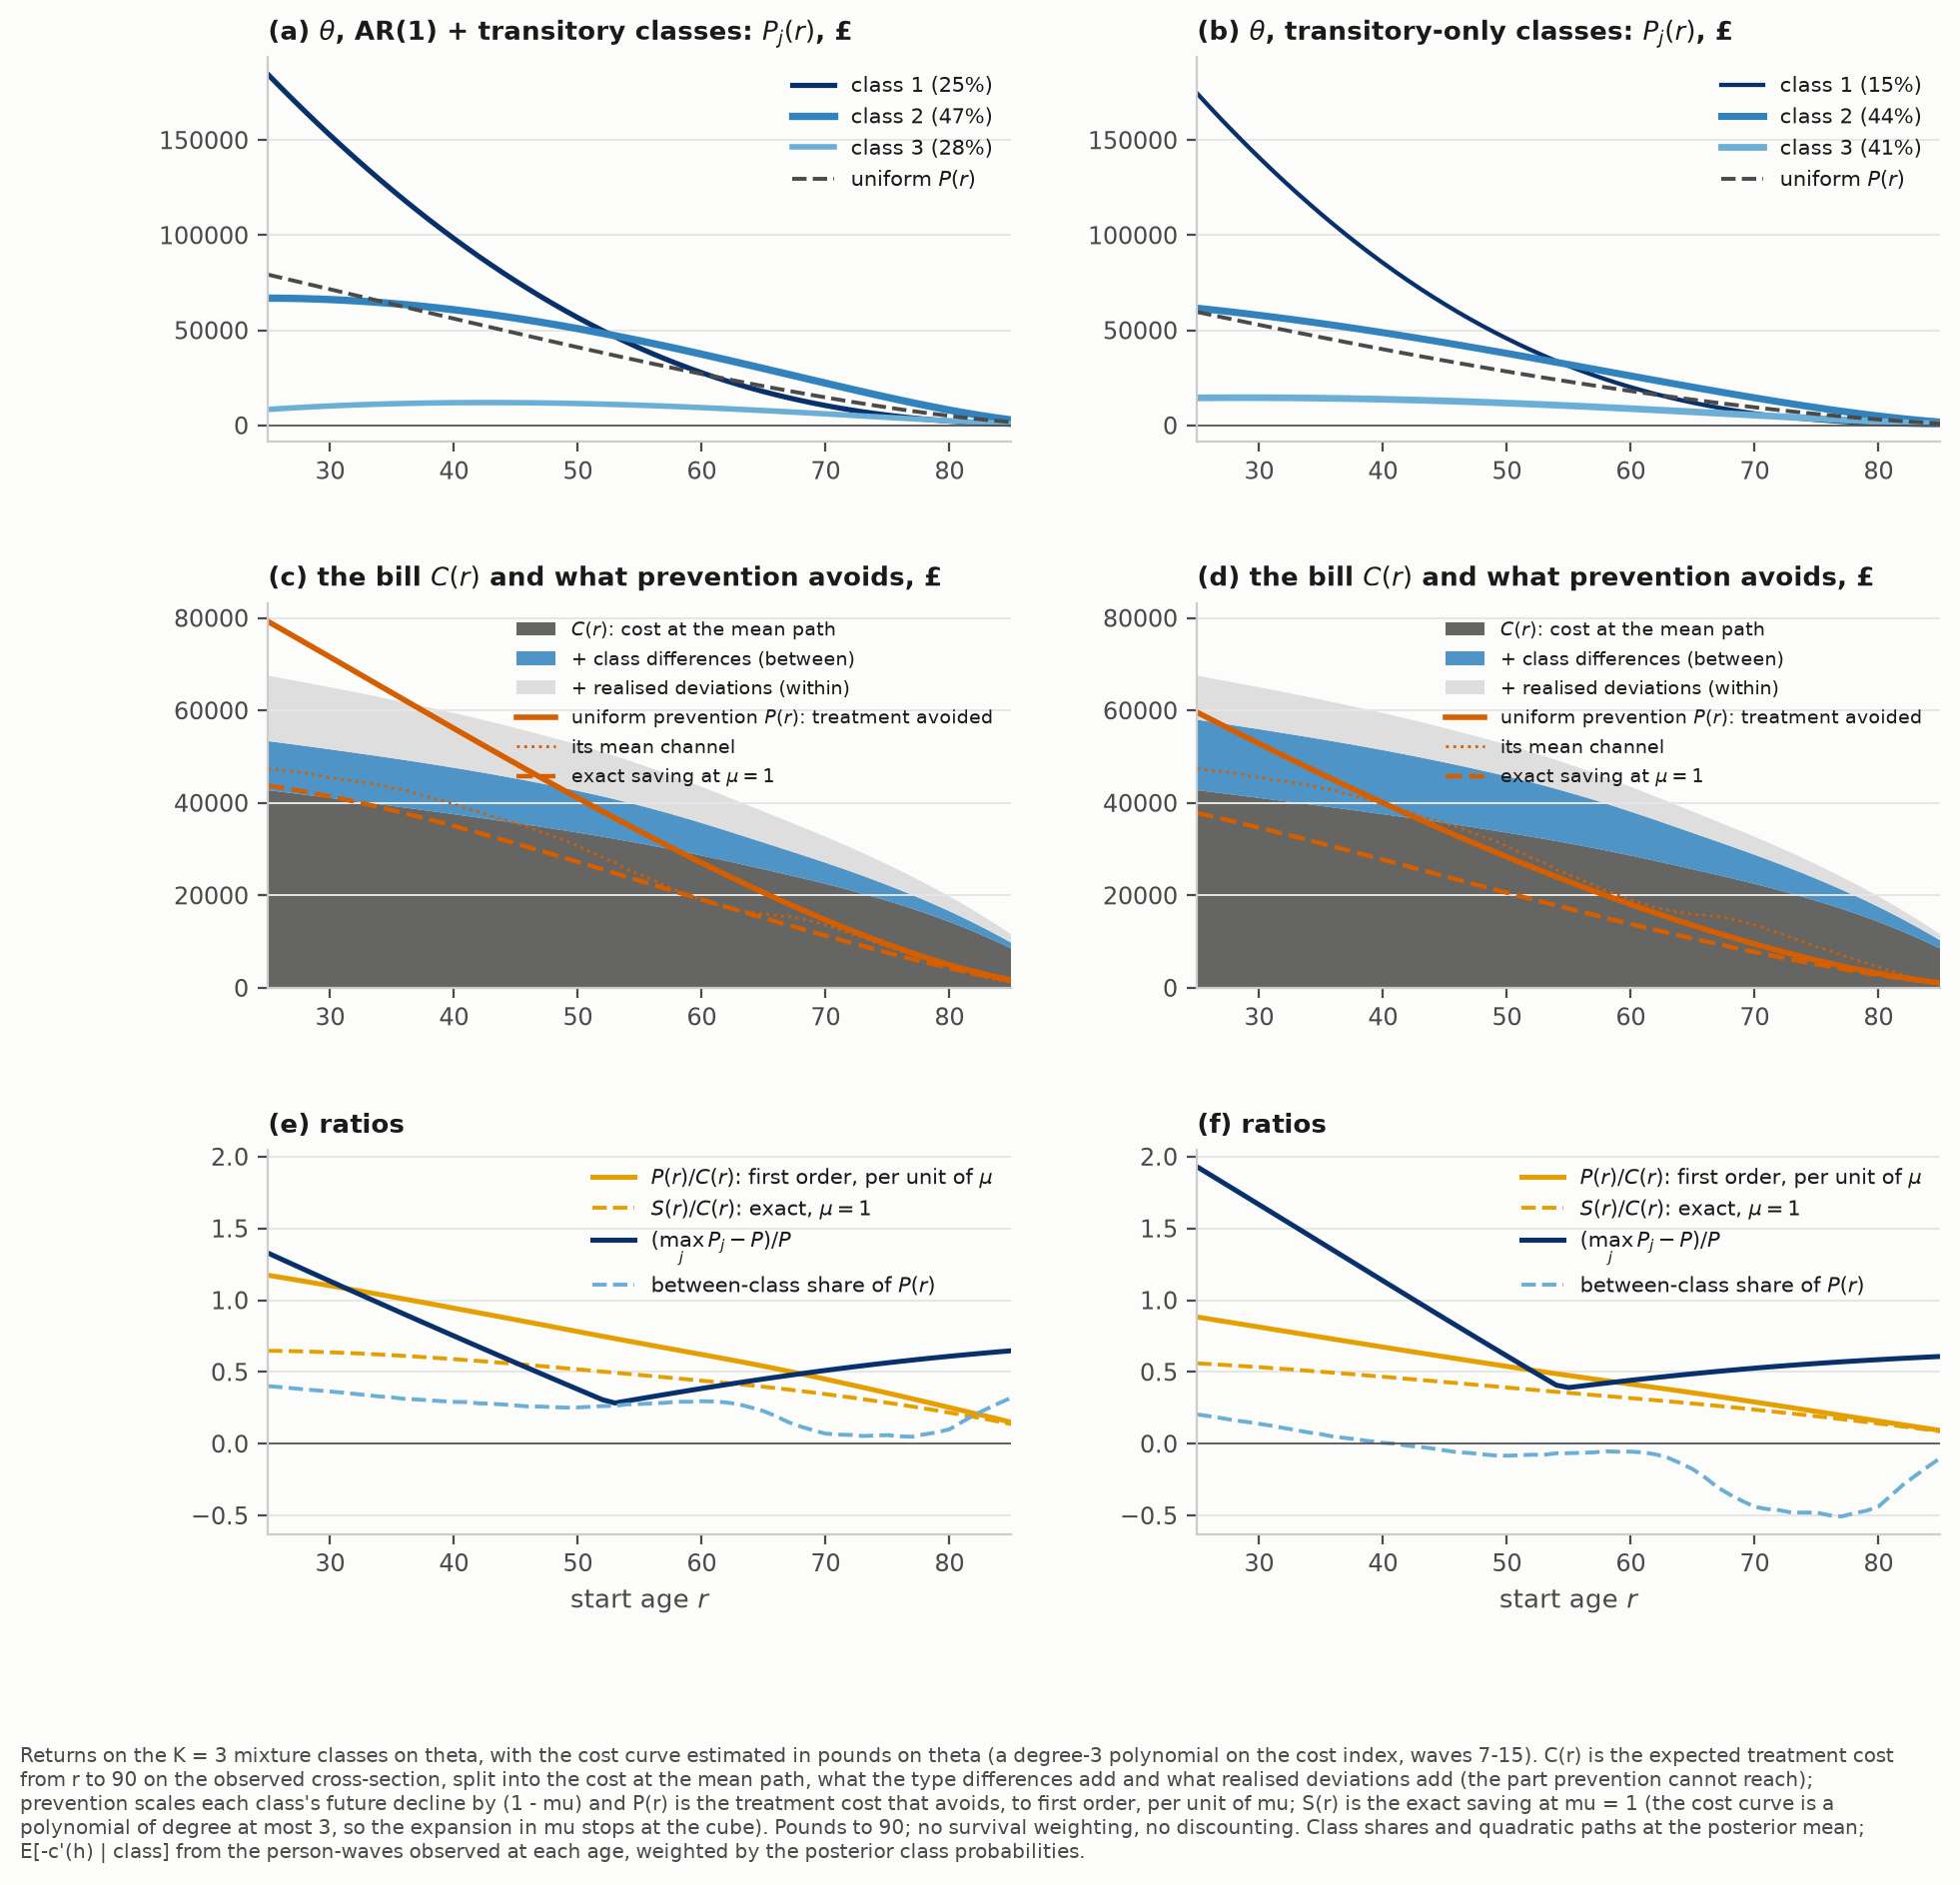
\includegraphics[width=\linewidth]{fig_returns_bayes.png}
	\caption{Bill, $P_j(r)$, $P(r)$, $S(r)$ and ratios by start age; persistent--transitory (left) and transitory only (right).}
	\label{fig:returnsbayes}
\end{figure}
\begin{figure}[H]\centering
	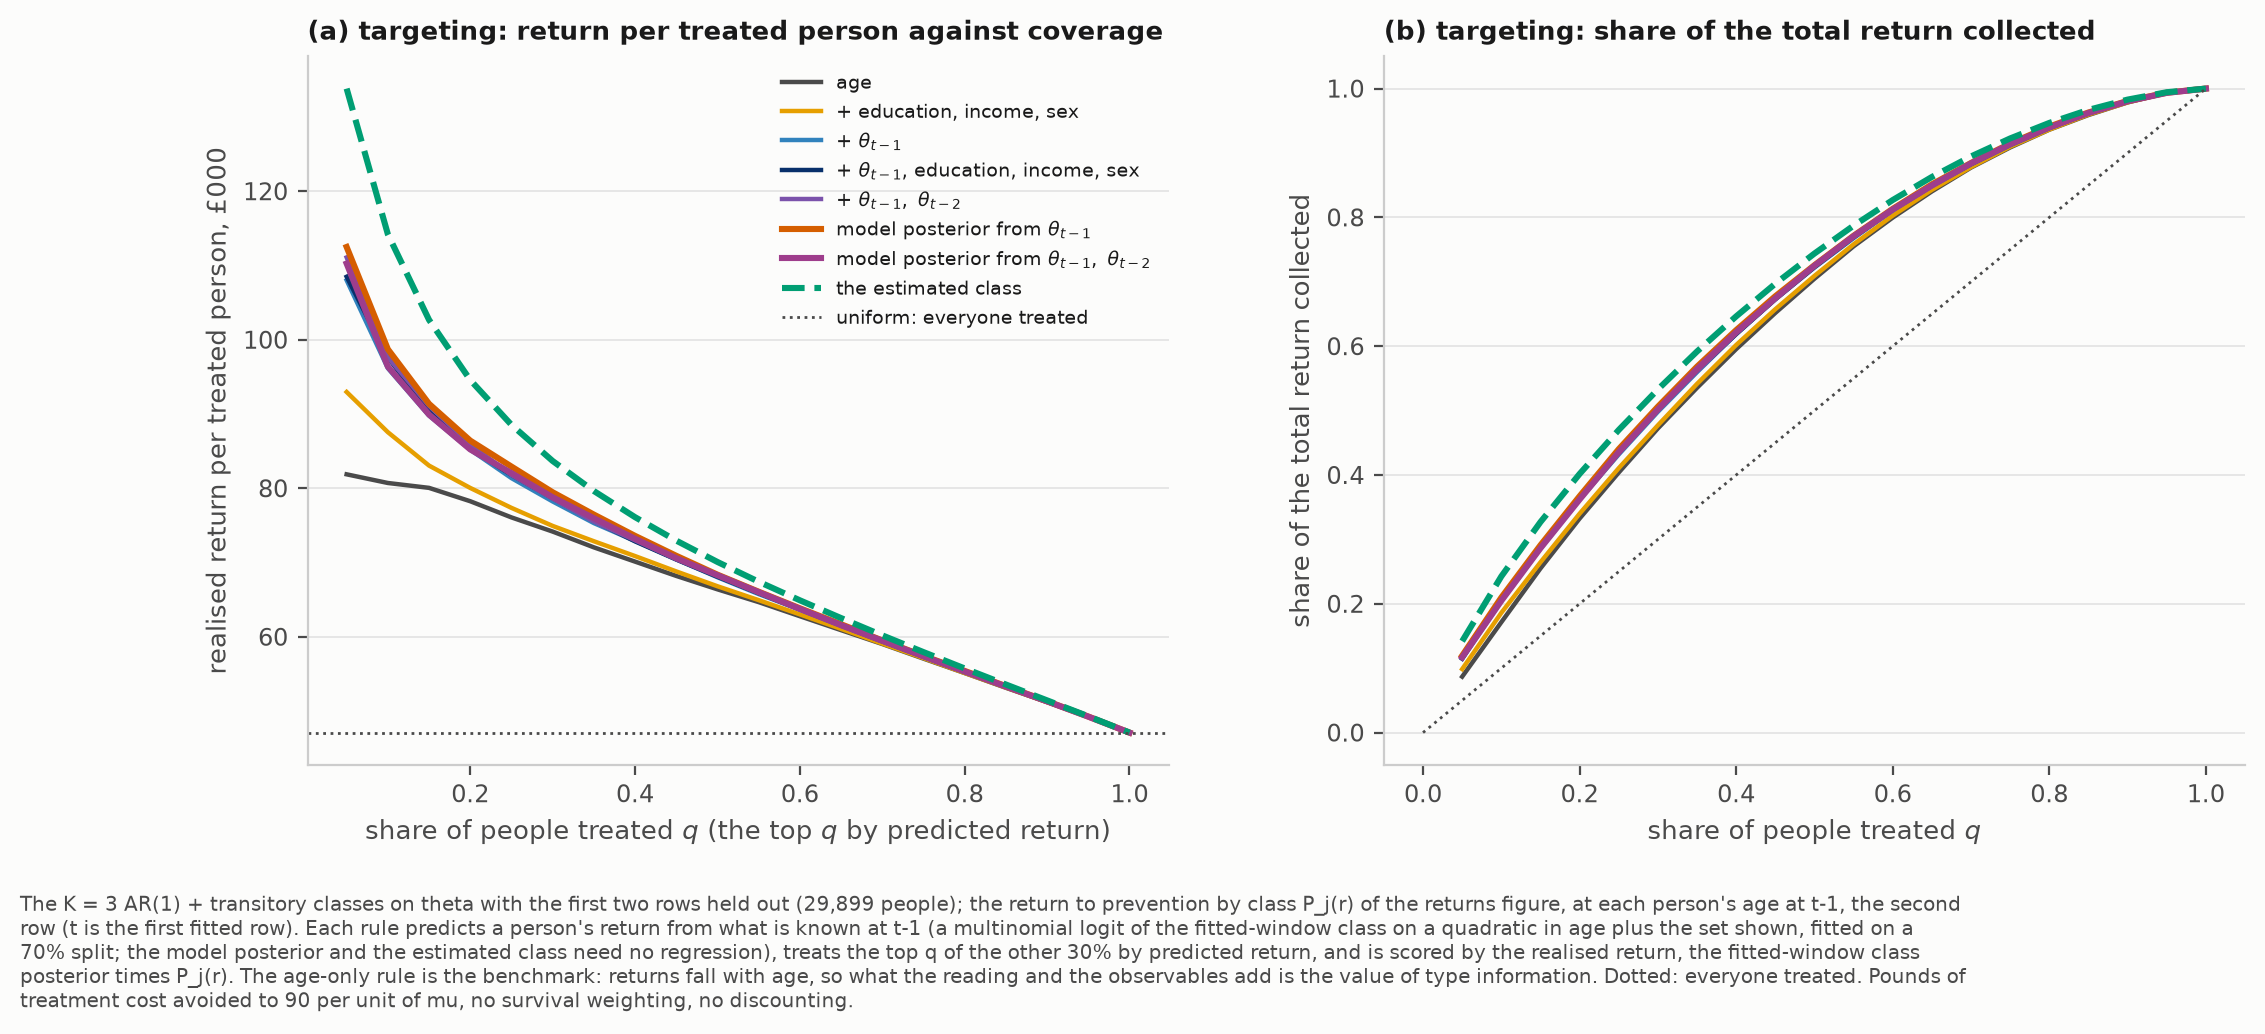
\includegraphics[width=\linewidth]{fig_targeting_first2.png}
	\caption{Targeting rules when the type is not observed: return per treated person and share collected.}
	\label{fig:targeting}
\end{figure}
\begin{figure}[H]\centering
	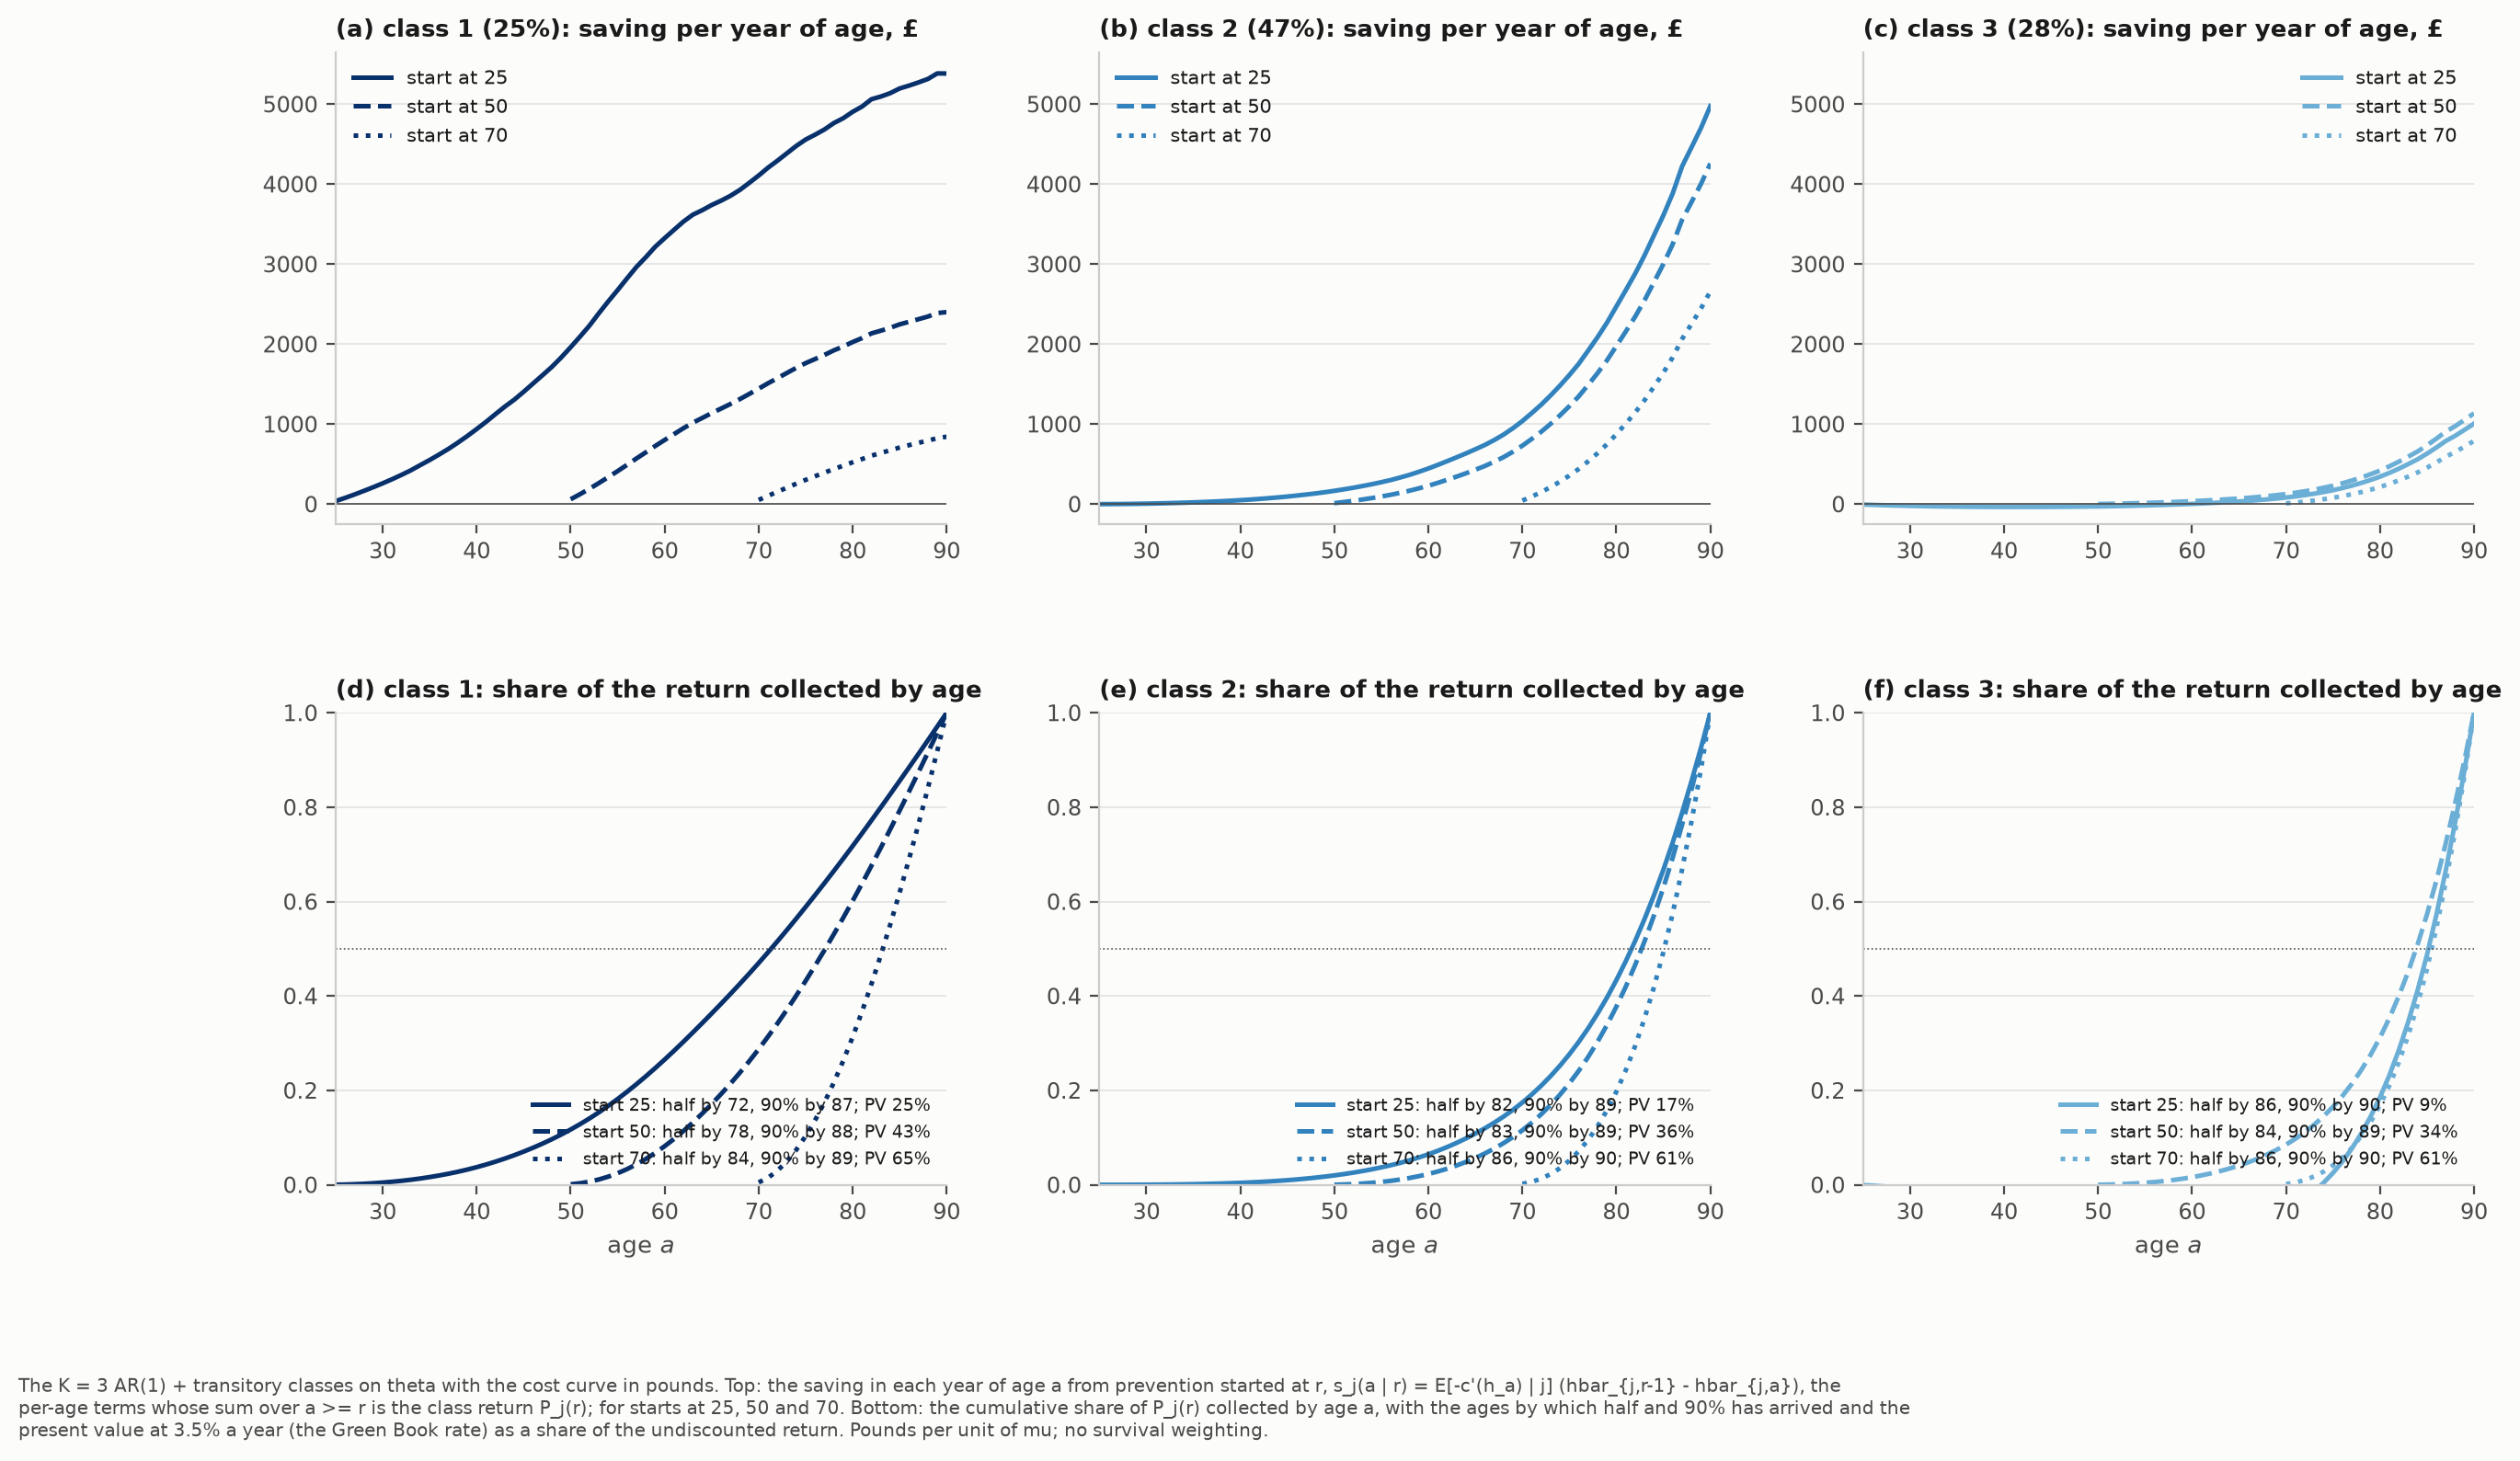
\includegraphics[width=\linewidth]{fig_prevention_timing.png}
	\caption{When the saving arrives by class, with half-way ages and present values at 3.5\%.}
	\label{fig:timing}
\end{figure}

\subsection{K-Means Types under the Estimated Cost Curve}
\label{app:returns_kmeans}
\begin{itemize}
	\item Lower $P/C$ than the mixture, and the between-type channel turns negative from about 40.
\end{itemize}
\begin{figure}[H]\centering
	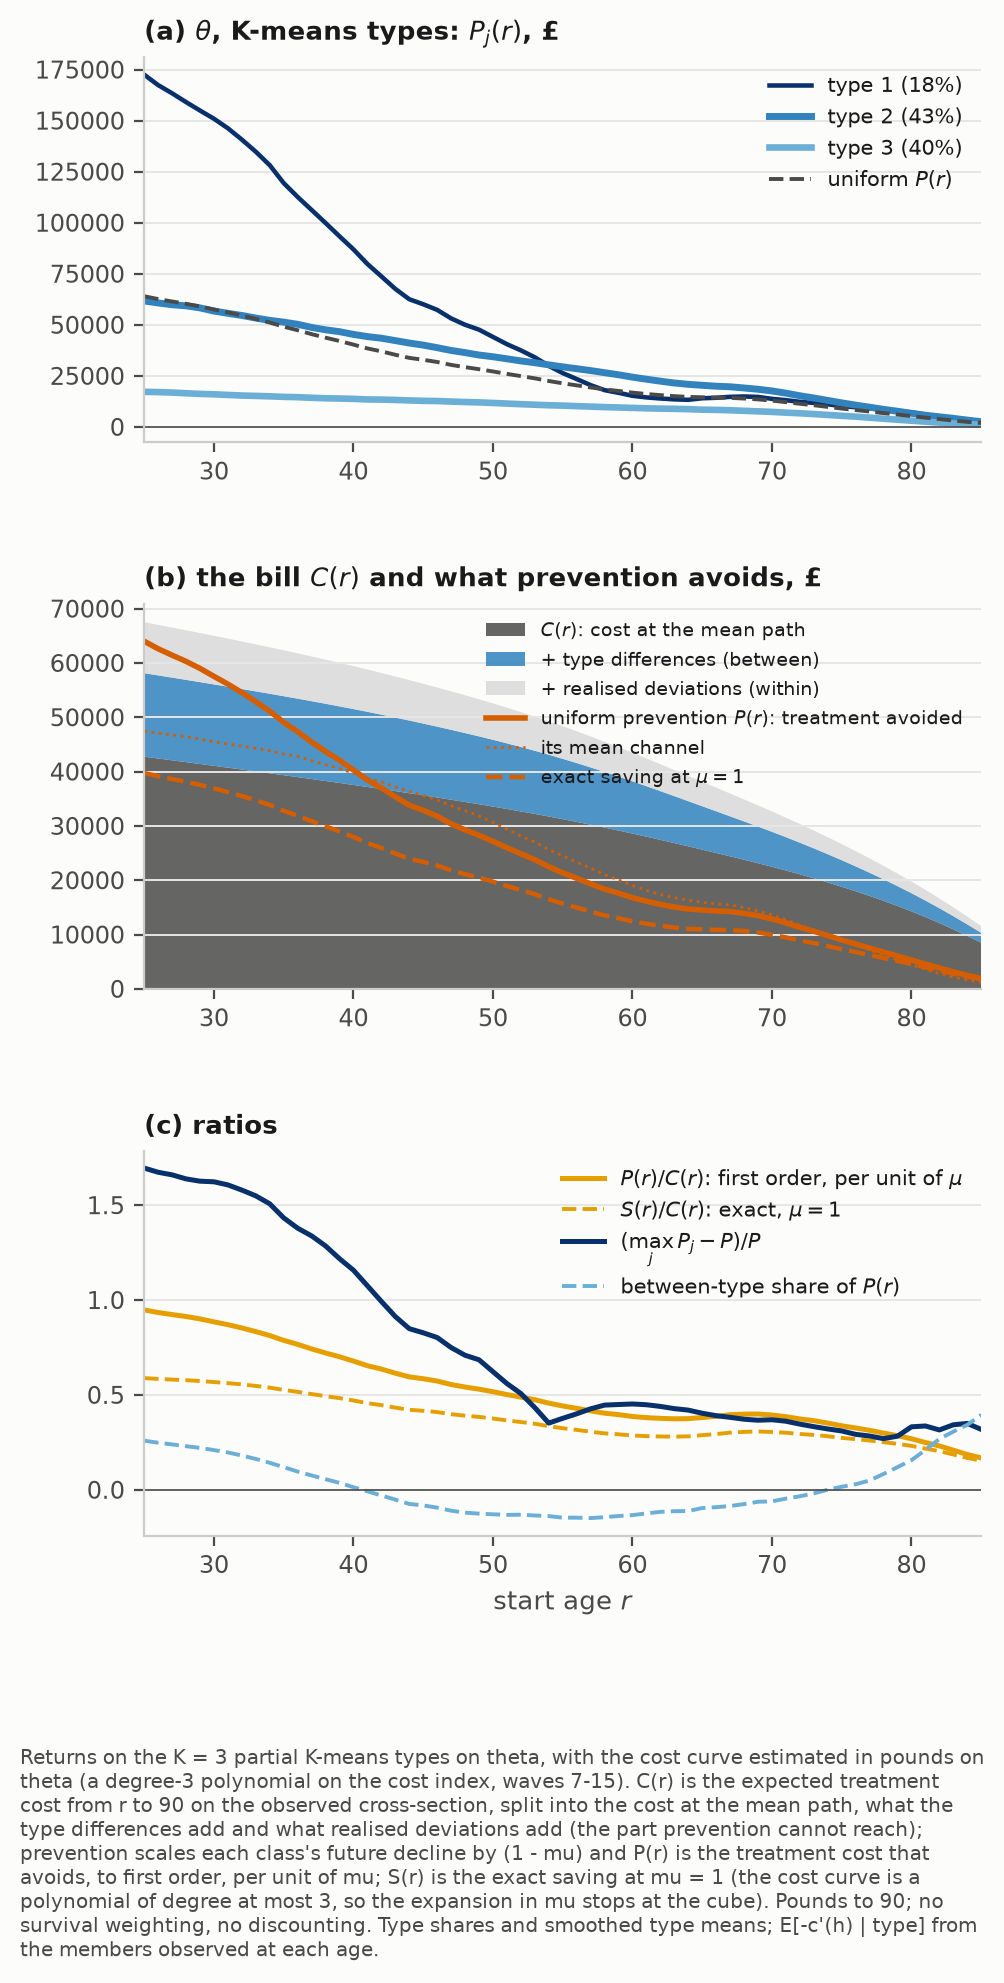
\includegraphics[width=0.55\linewidth]{fig_returns_bayes_kmeans.png}
	\caption{As Figure~\ref{fig:returnsbayes}, on the K-means types.}
	\label{fig:returnskmeans}
\end{figure}

\subsection{The Capped Cost Curve}
\label{app:returns_capped}
\begin{itemize}
	\item Capping roughly halves first-order returns; the ranking survives.
\end{itemize}
\begin{figure}[H]\centering
	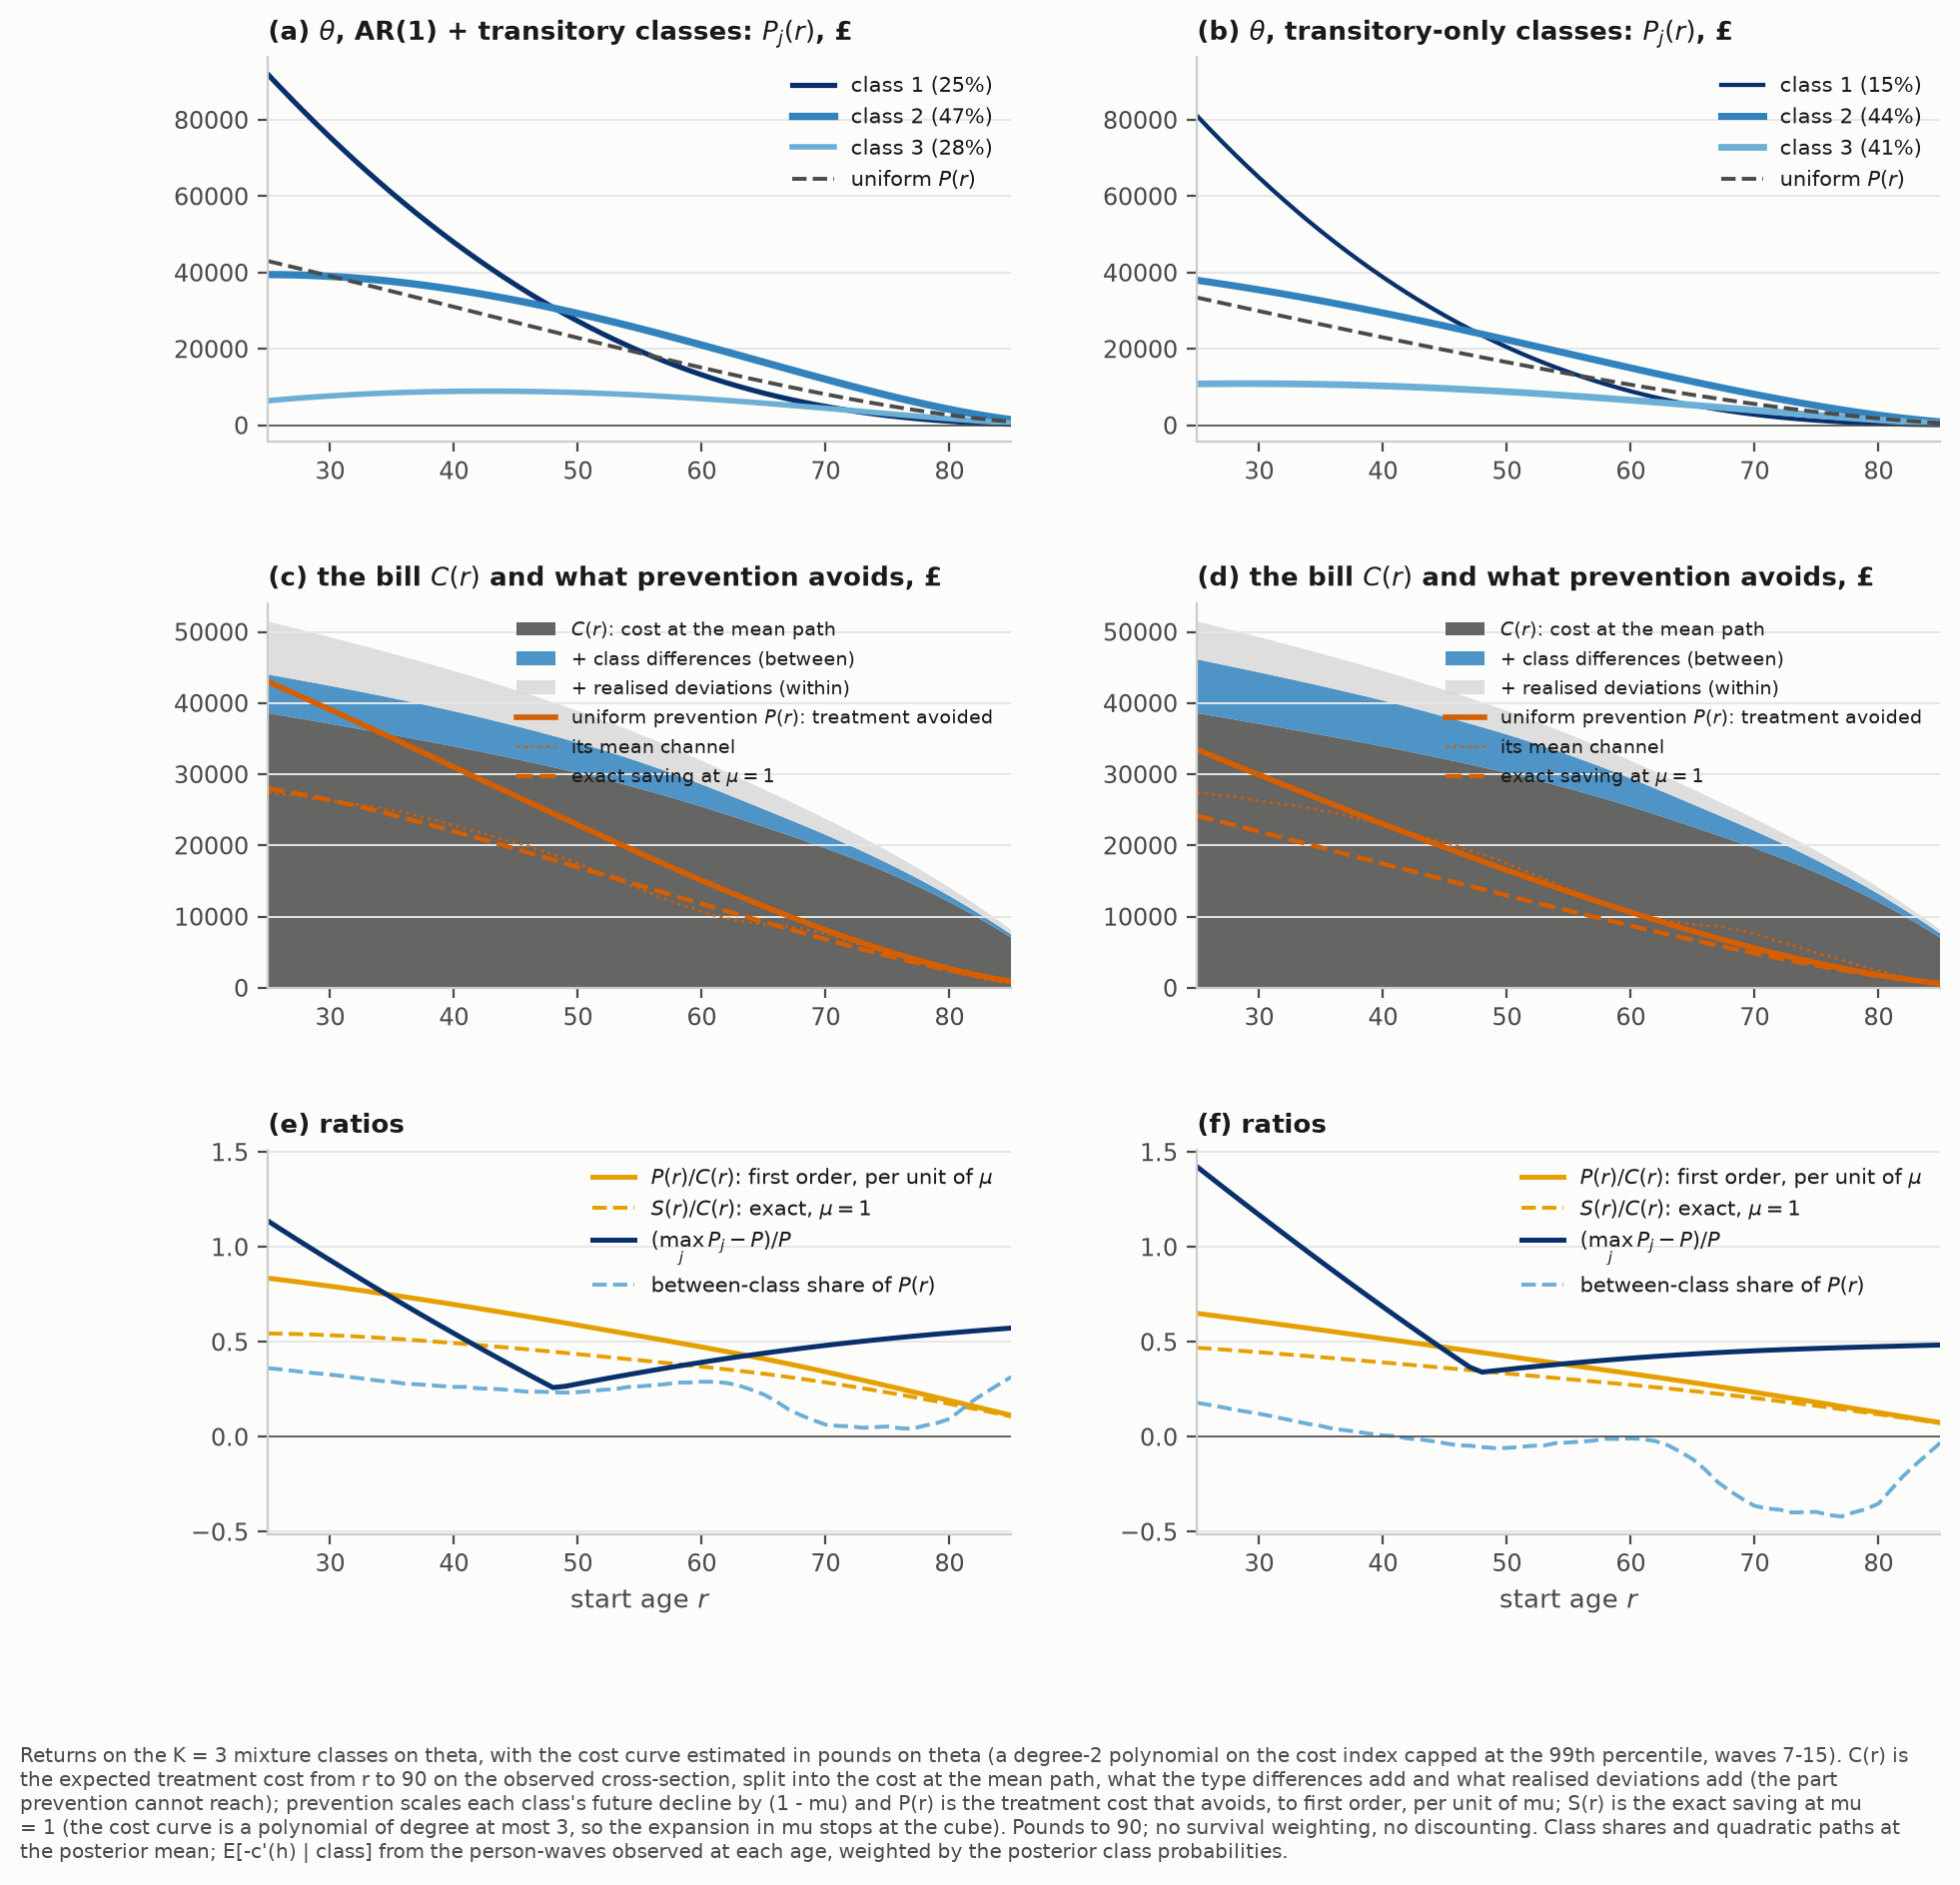
\includegraphics[width=\linewidth]{fig_returns_bayes_capped.png}
	\caption{As Figure~\ref{fig:returnsbayes}, with costs capped at the 99th percentile.}
	\label{fig:returnscapped}
\end{figure}

\subsection{The Return by Class under Other Typologies and Measures}
\label{app:returns_models}
\begin{itemize}
	\item Same shape under every typology; decade shifts raise returns by about a quarter; the worst class carries the return on every measure; adding classes splits the return, it does not create it.
\end{itemize}
\begin{figure}[H]\centering
	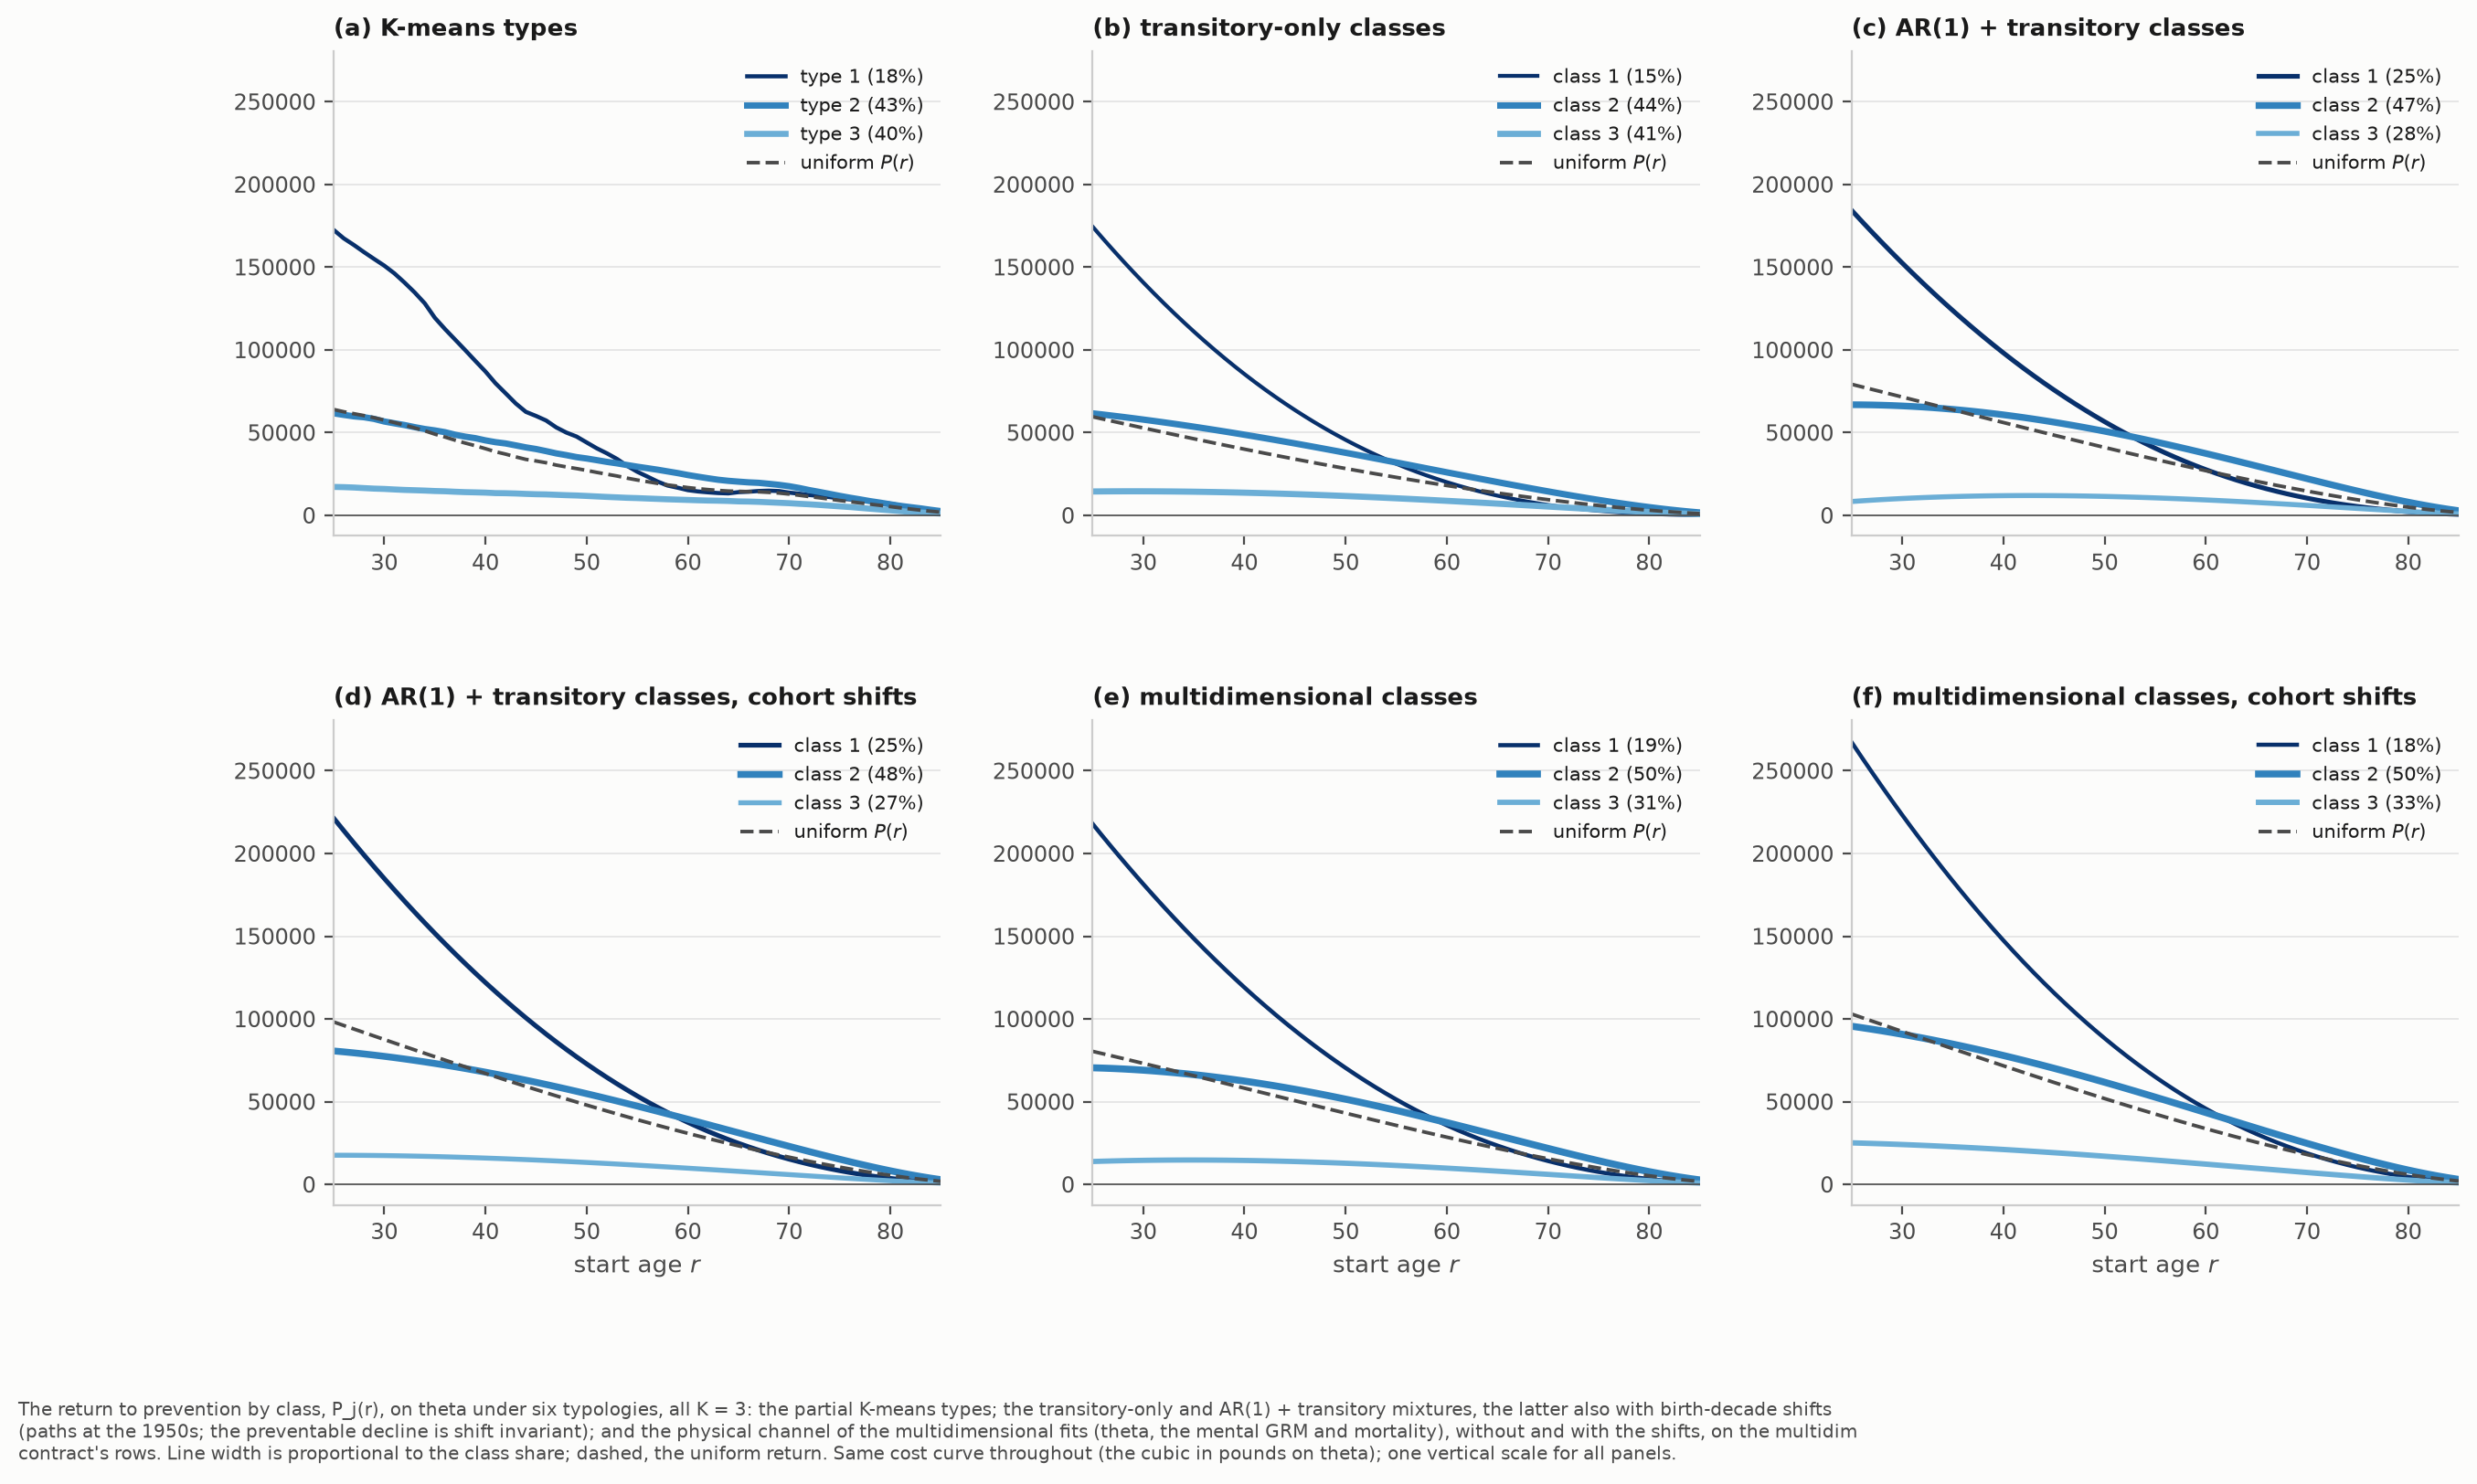
\includegraphics[width=\linewidth]{fig_returns_by_model.png}
	\caption{$P_j(r)$ under six typologies on $\theta$.}
	\label{fig:returnsmodels}
\end{figure}
\begin{figure}[H]\centering
	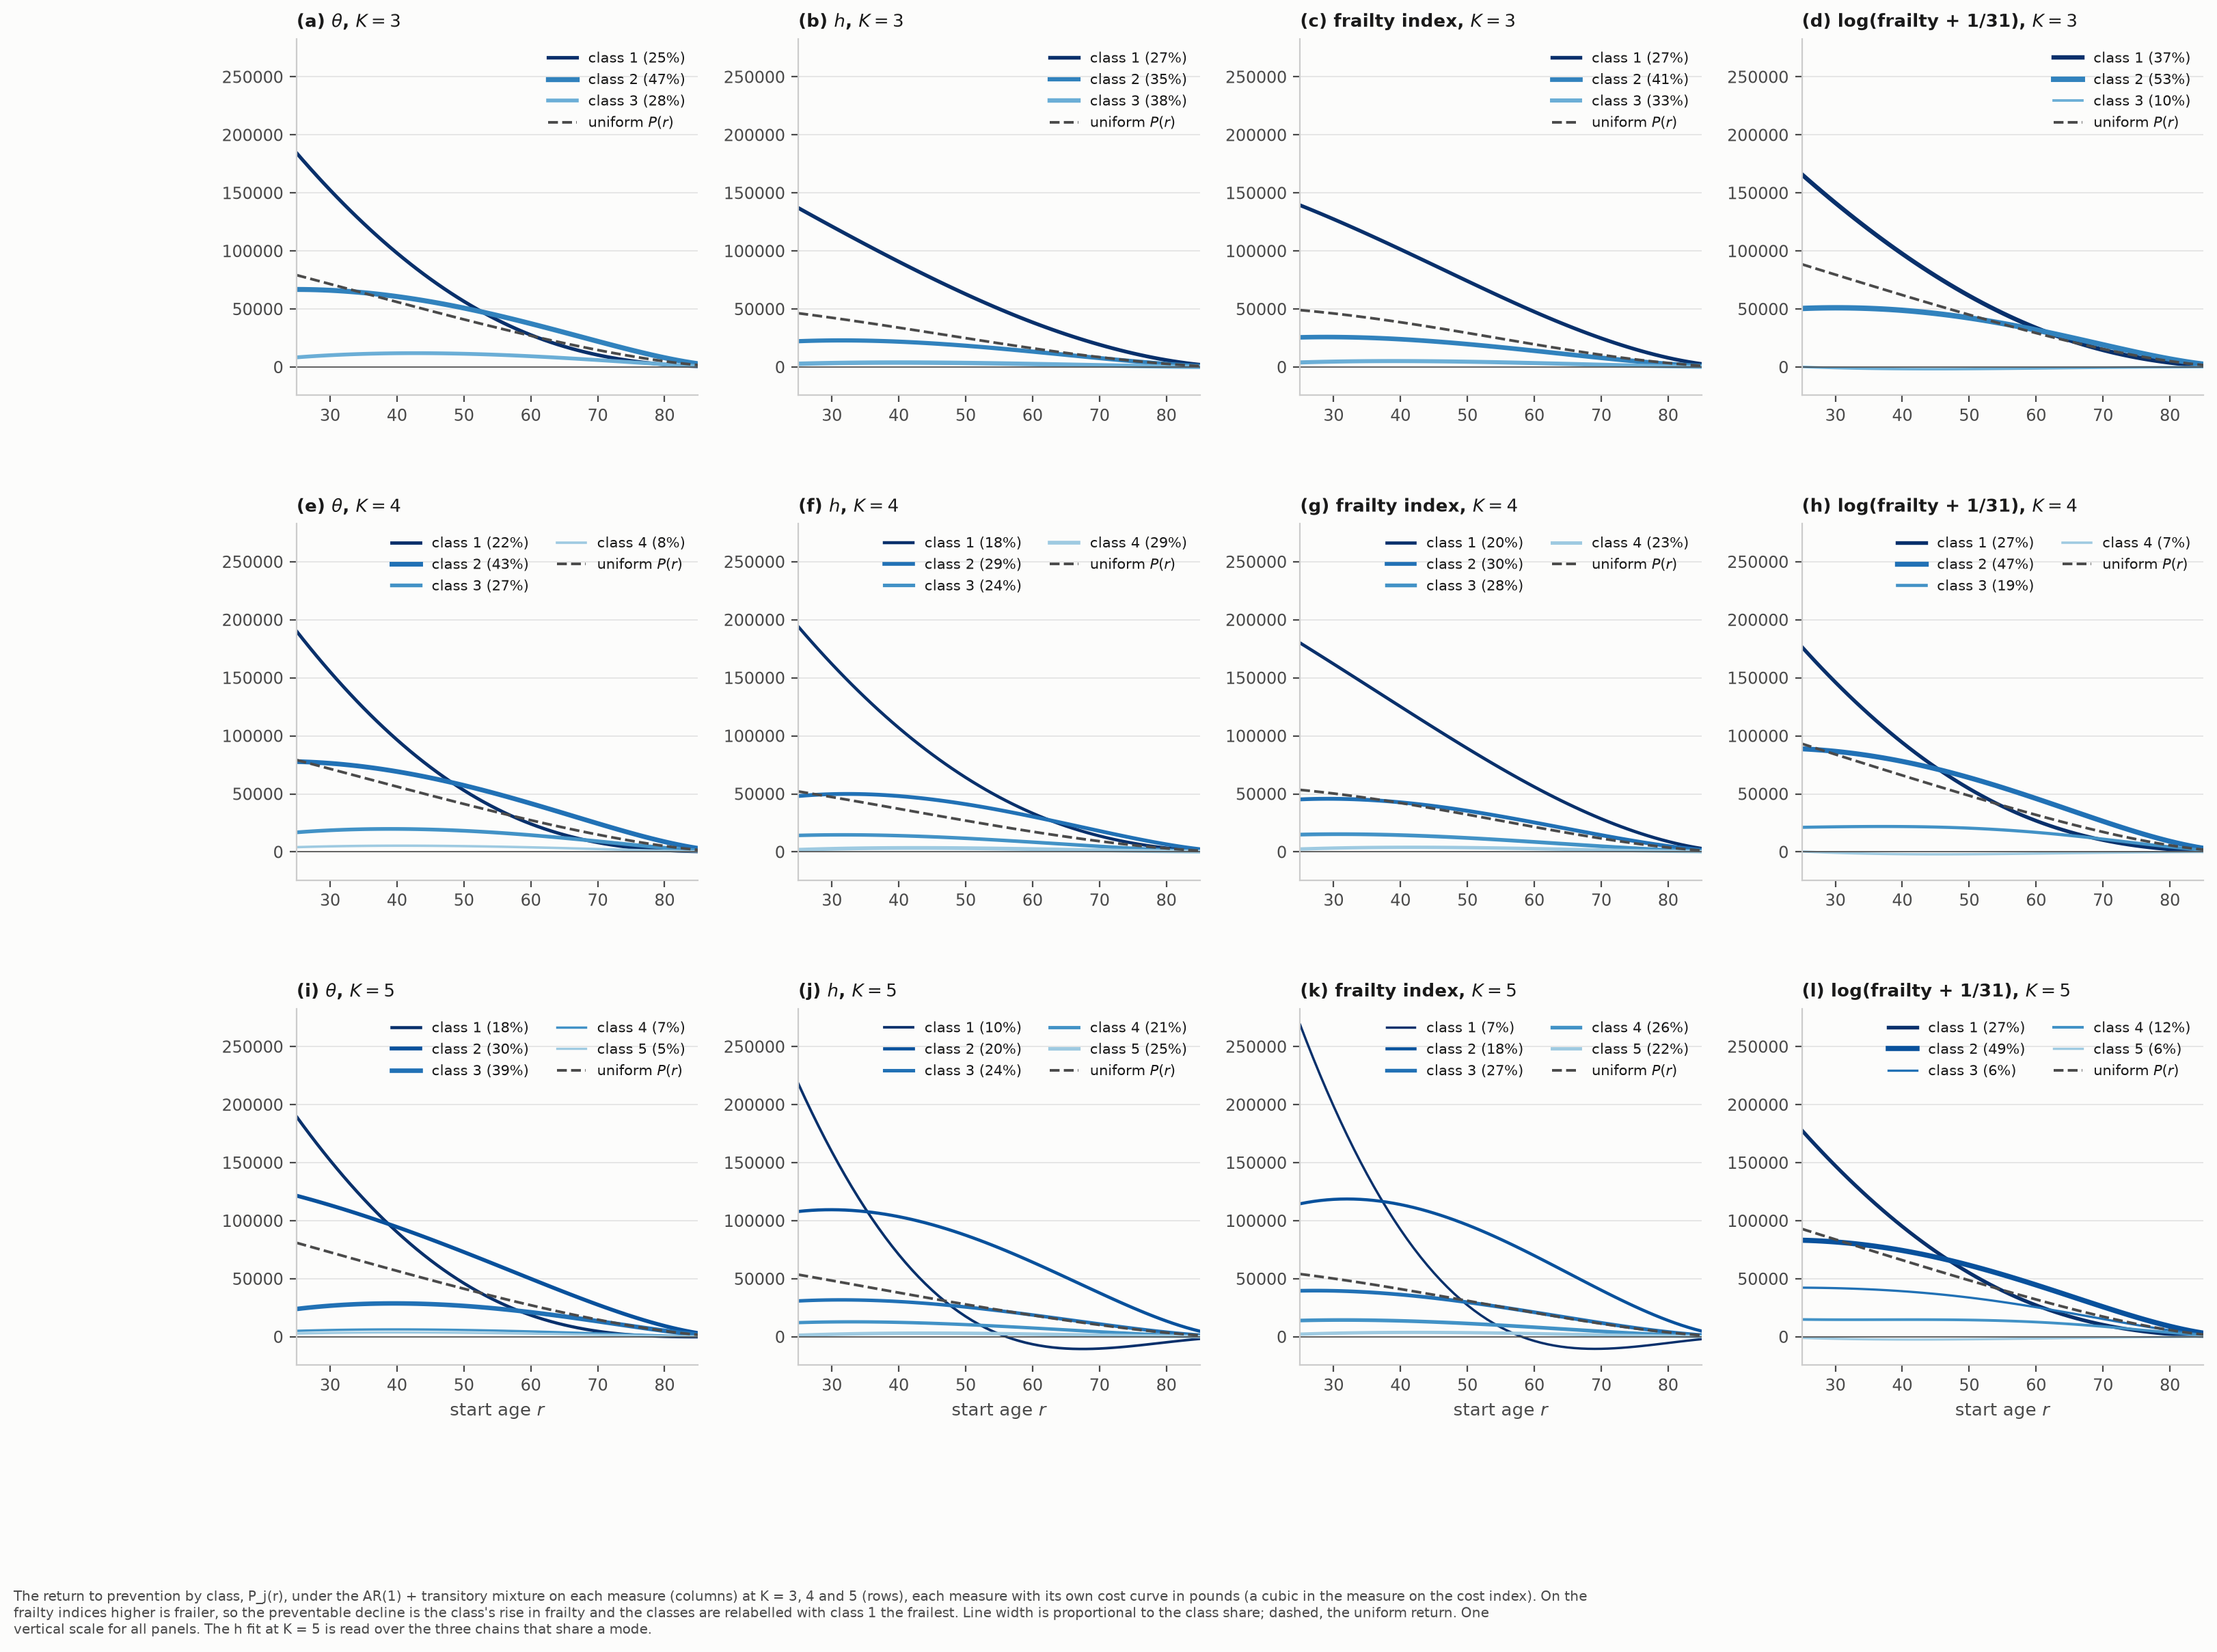
\includegraphics[width=\linewidth]{fig_returns_by_measure.png}
	\caption{$P_j(r)$ on each of the four measures at $K=3,4,5$.}
	\label{fig:returnsmeasures}
\end{figure}

\subsection{Life Years}
\label{app:prevle}
\begin{itemize}
	\item Multidimensional classes give wider gaps and the same policy ranking; on the other measures targeting closes the gaps almost entirely.
\end{itemize}
\begin{figure}[H]\centering
	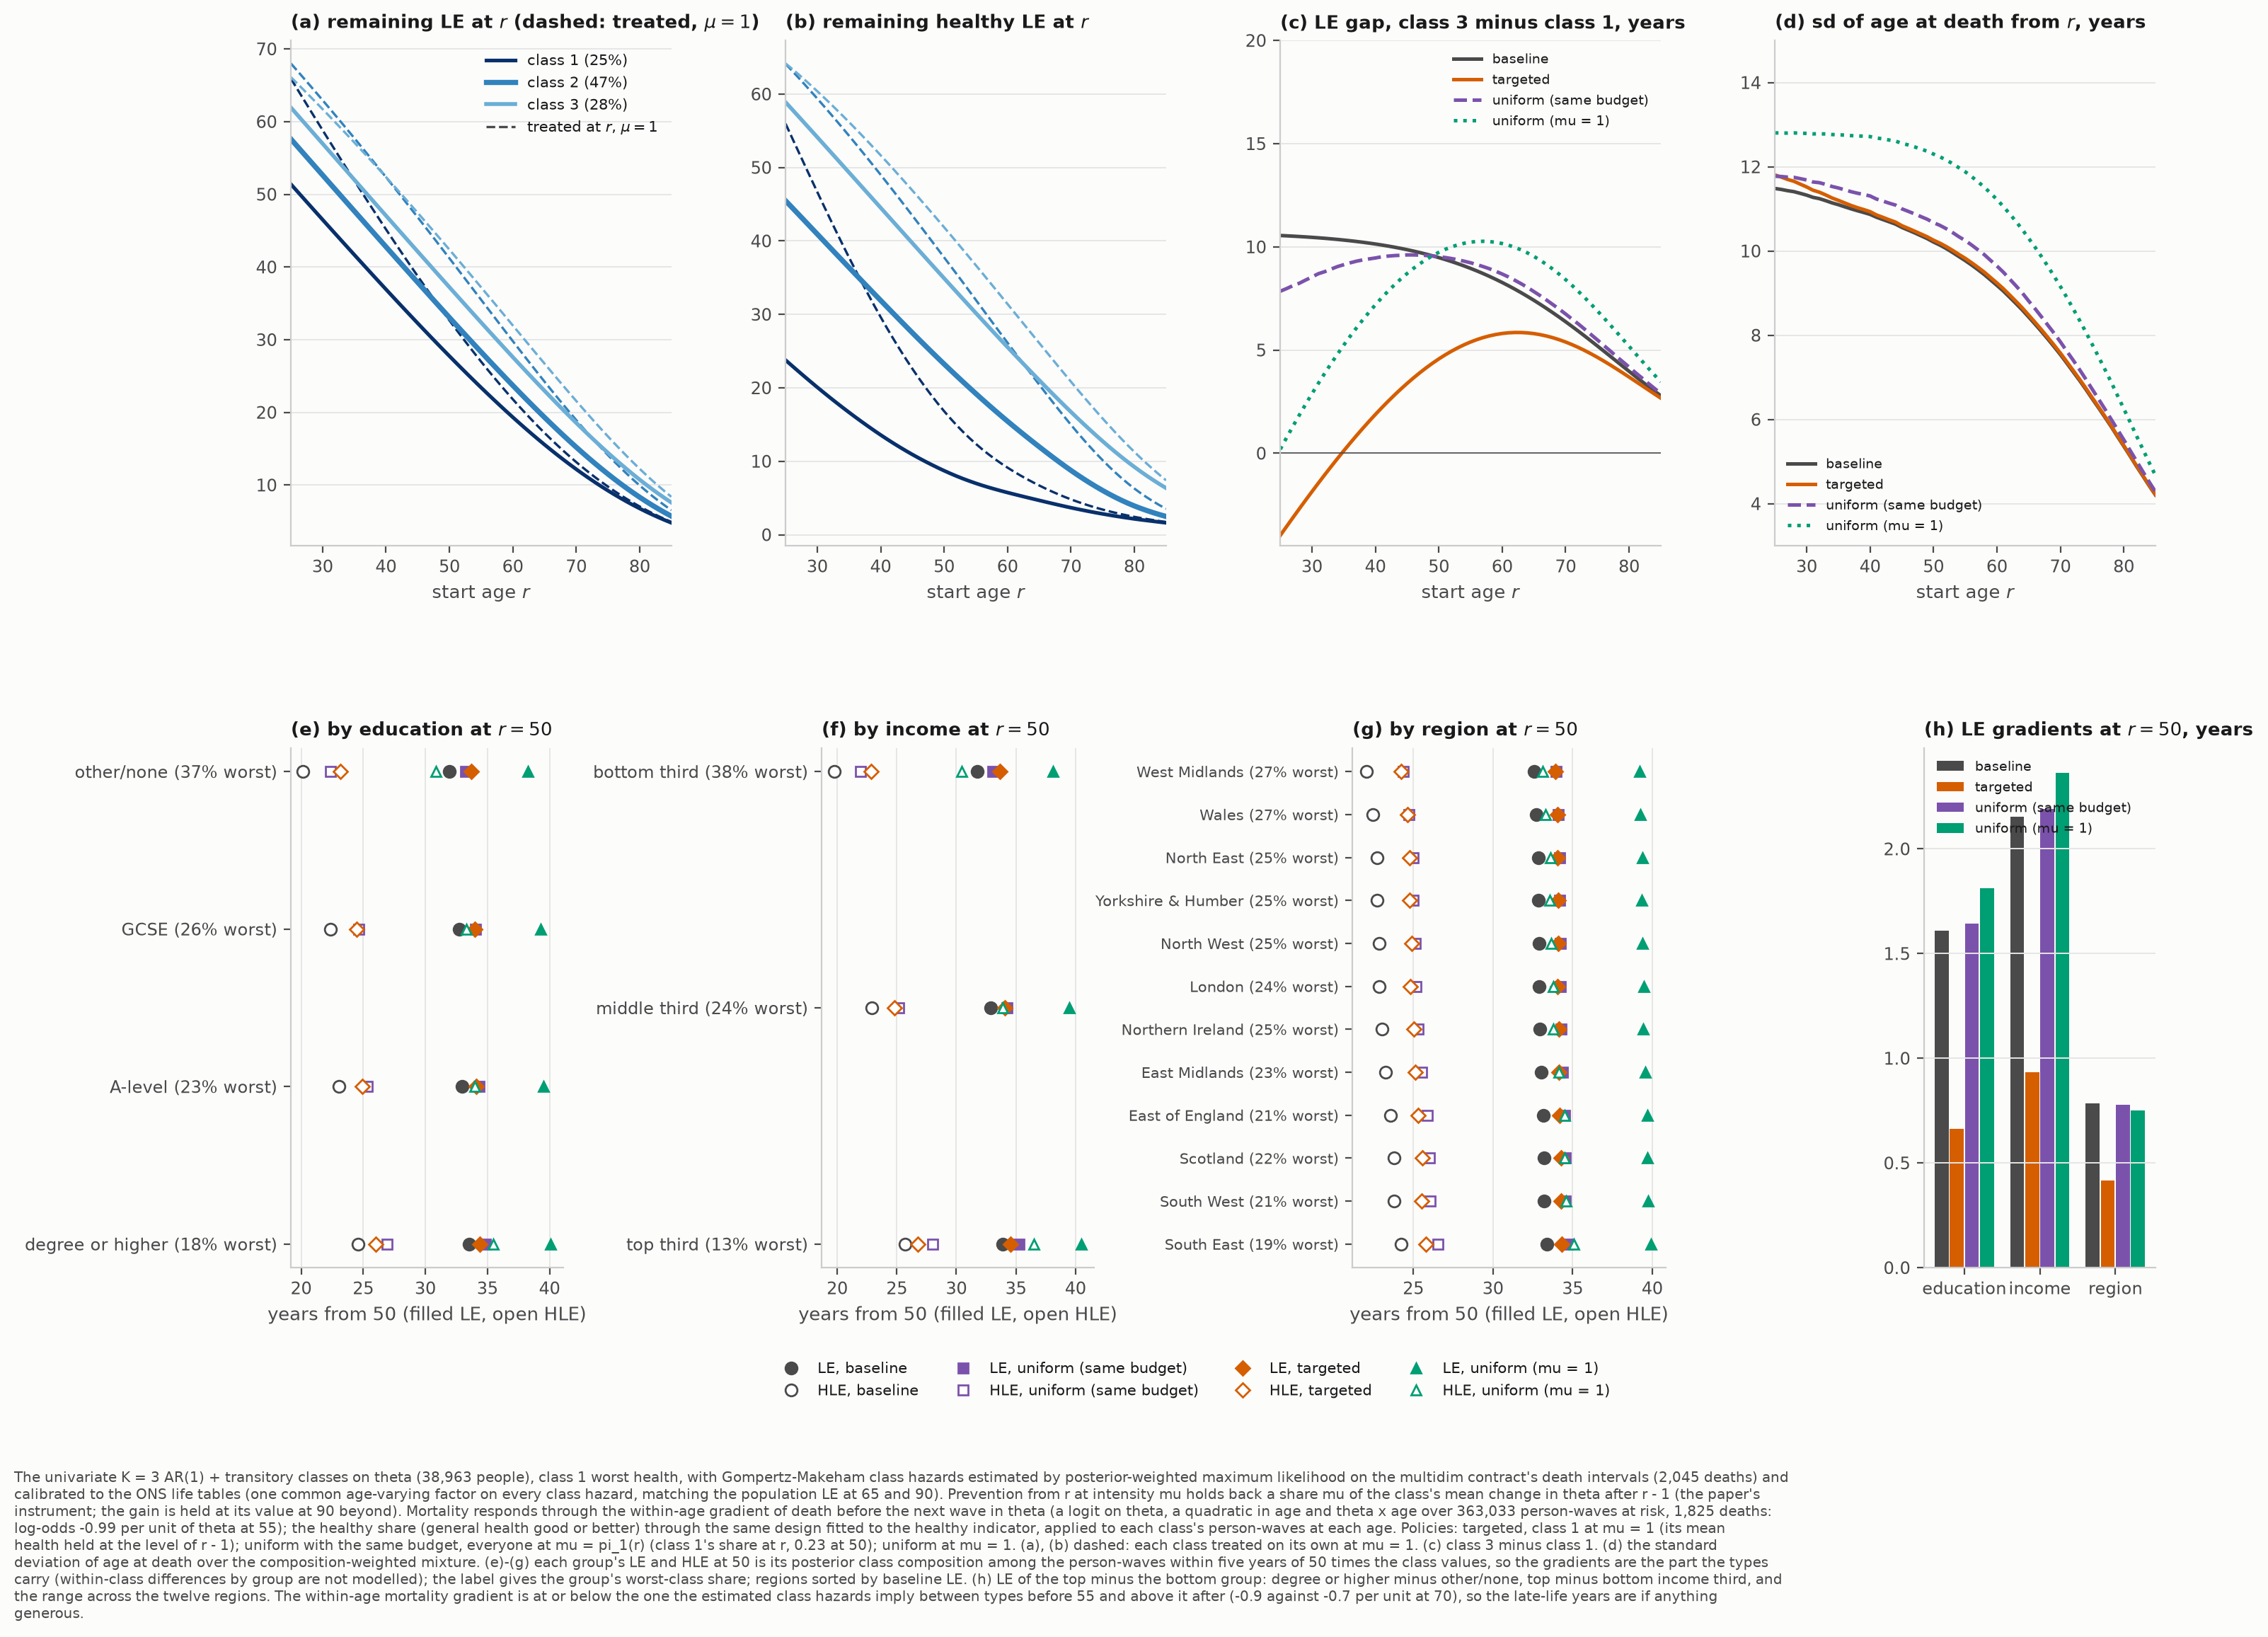
\includegraphics[width=\linewidth]{fig_prevention_le_uni.png}
	\caption{Detailed version of Figure~\ref{fig:prevle}.}
	\label{fig:prevle_uni}
\end{figure}
\begin{figure}[H]\centering
	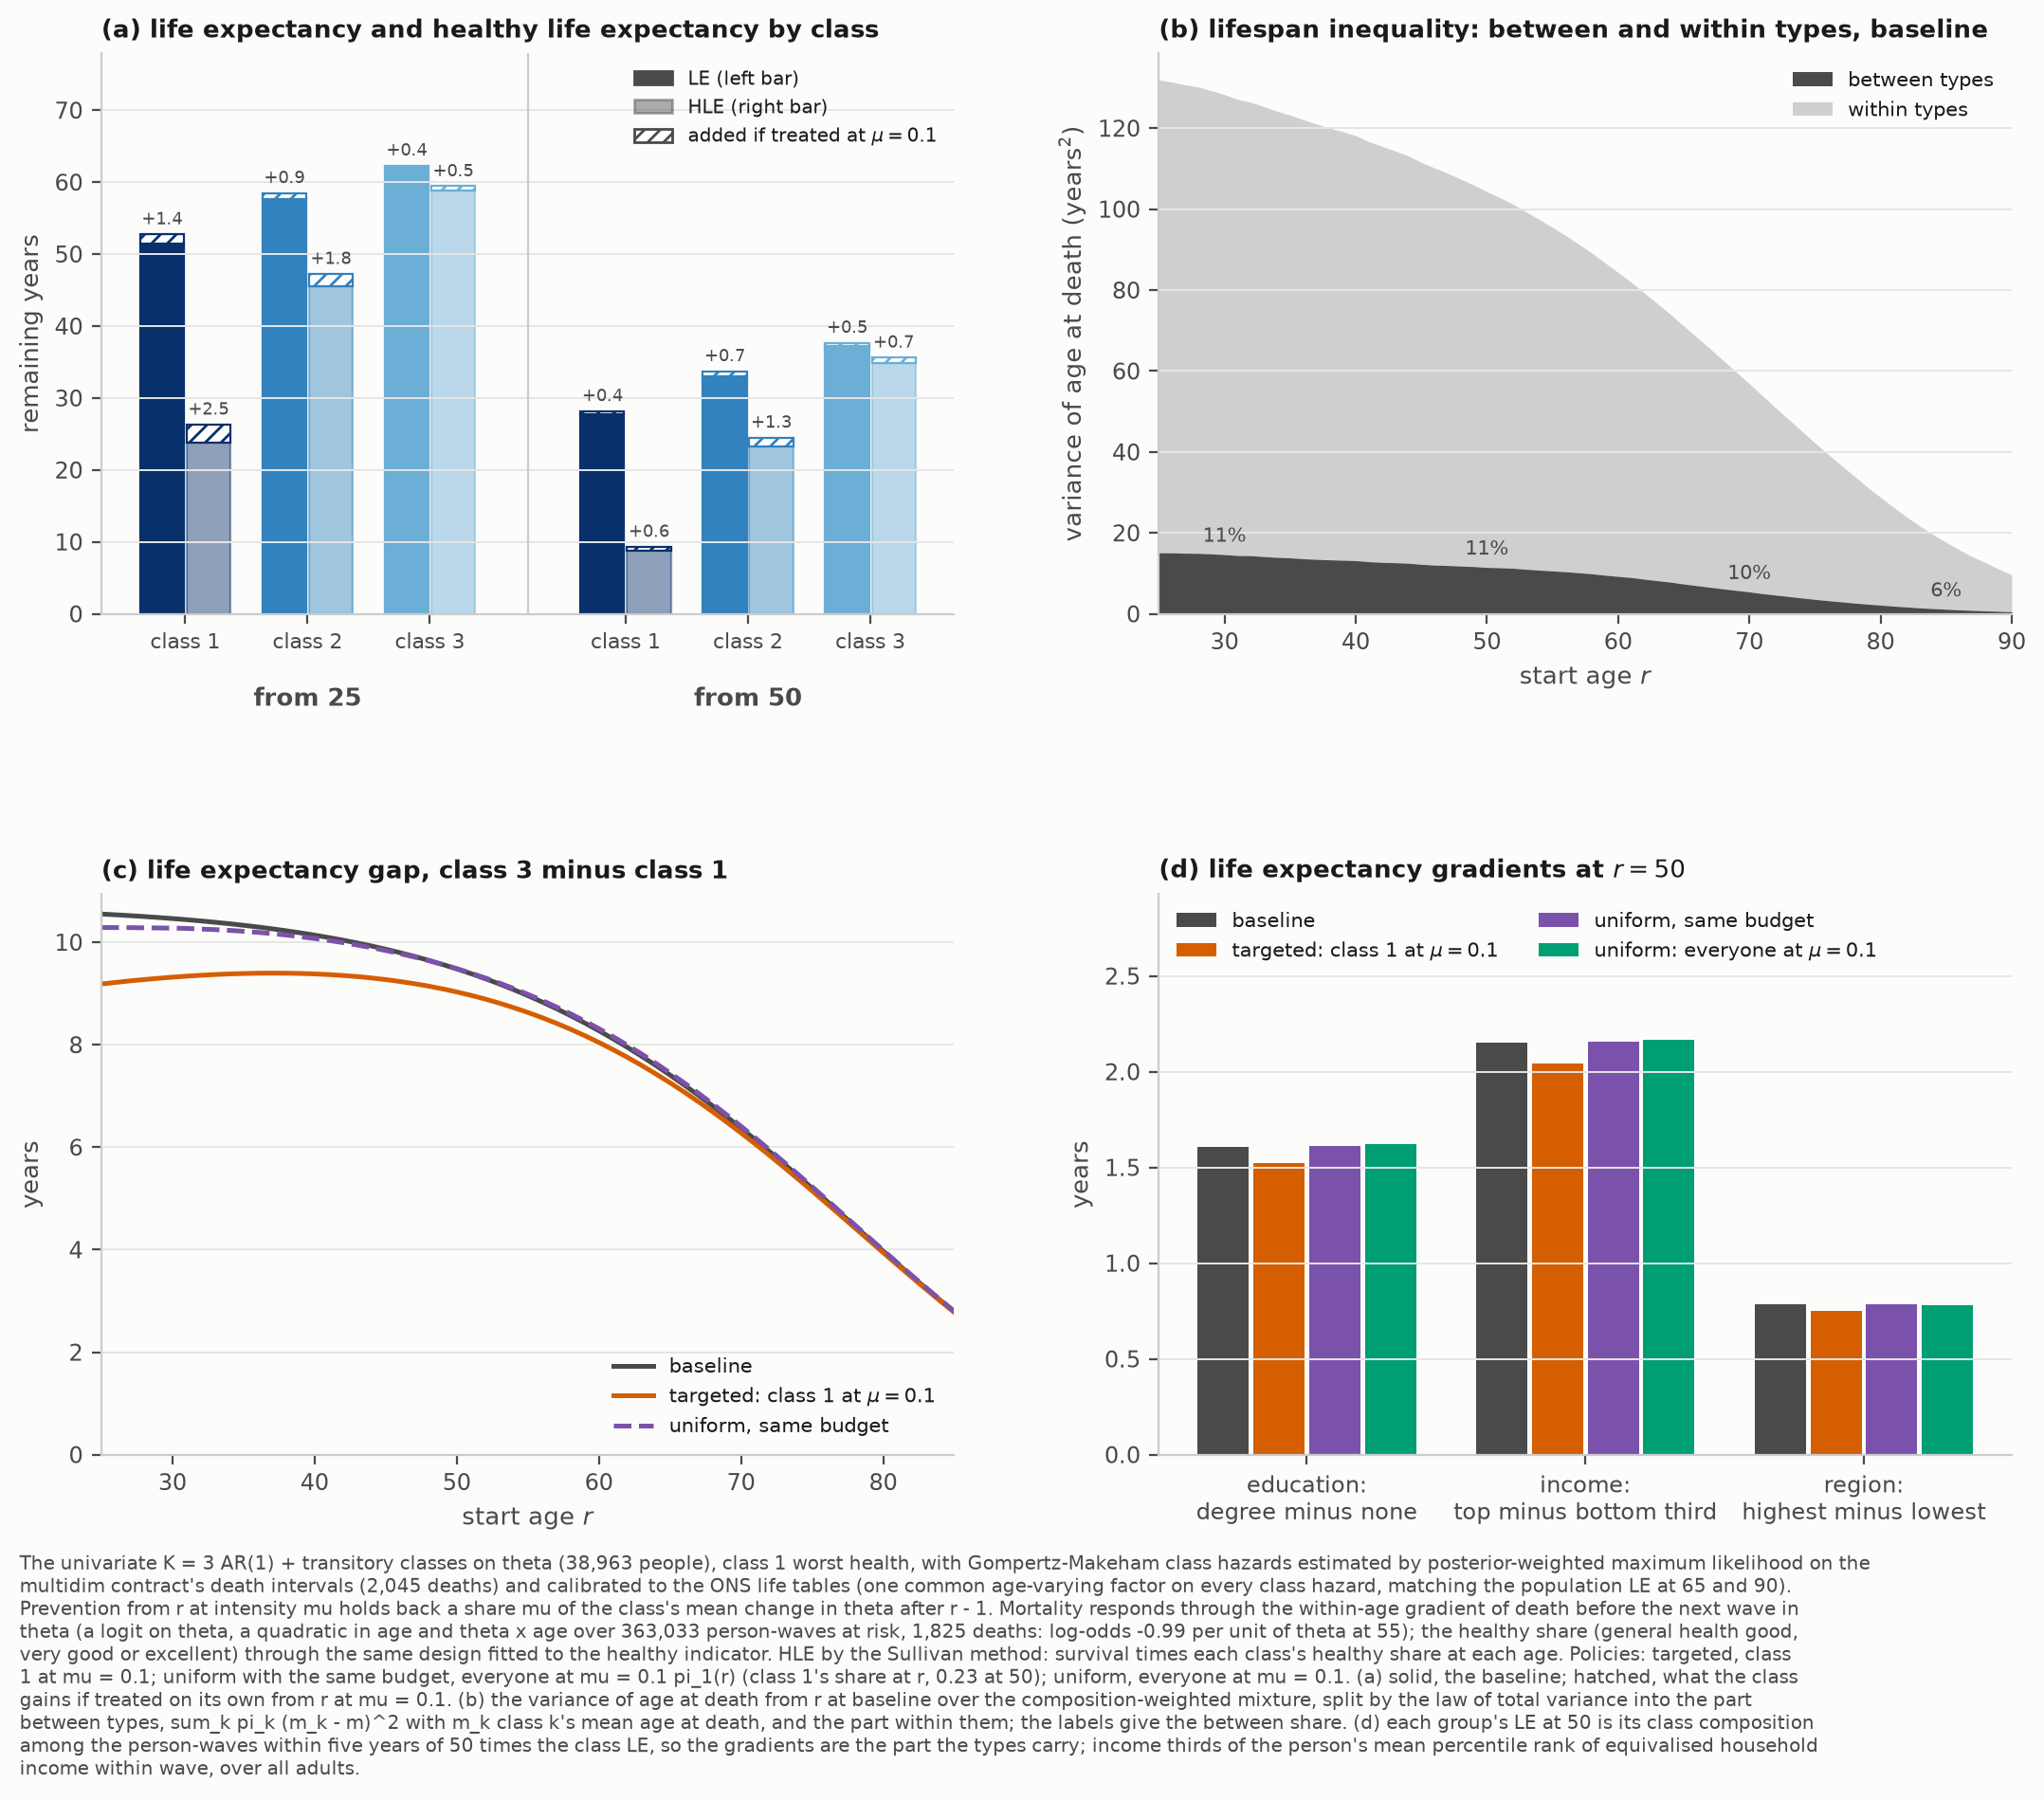
\includegraphics[width=\linewidth]{fig_prevention_le_uni_mu0.1_main.png}
	\caption{As Figure~\ref{fig:prevle}, at $\mu=0.1$.}
	\label{fig:prevle_mu01}
\end{figure}
\begin{figure}[H]\centering
	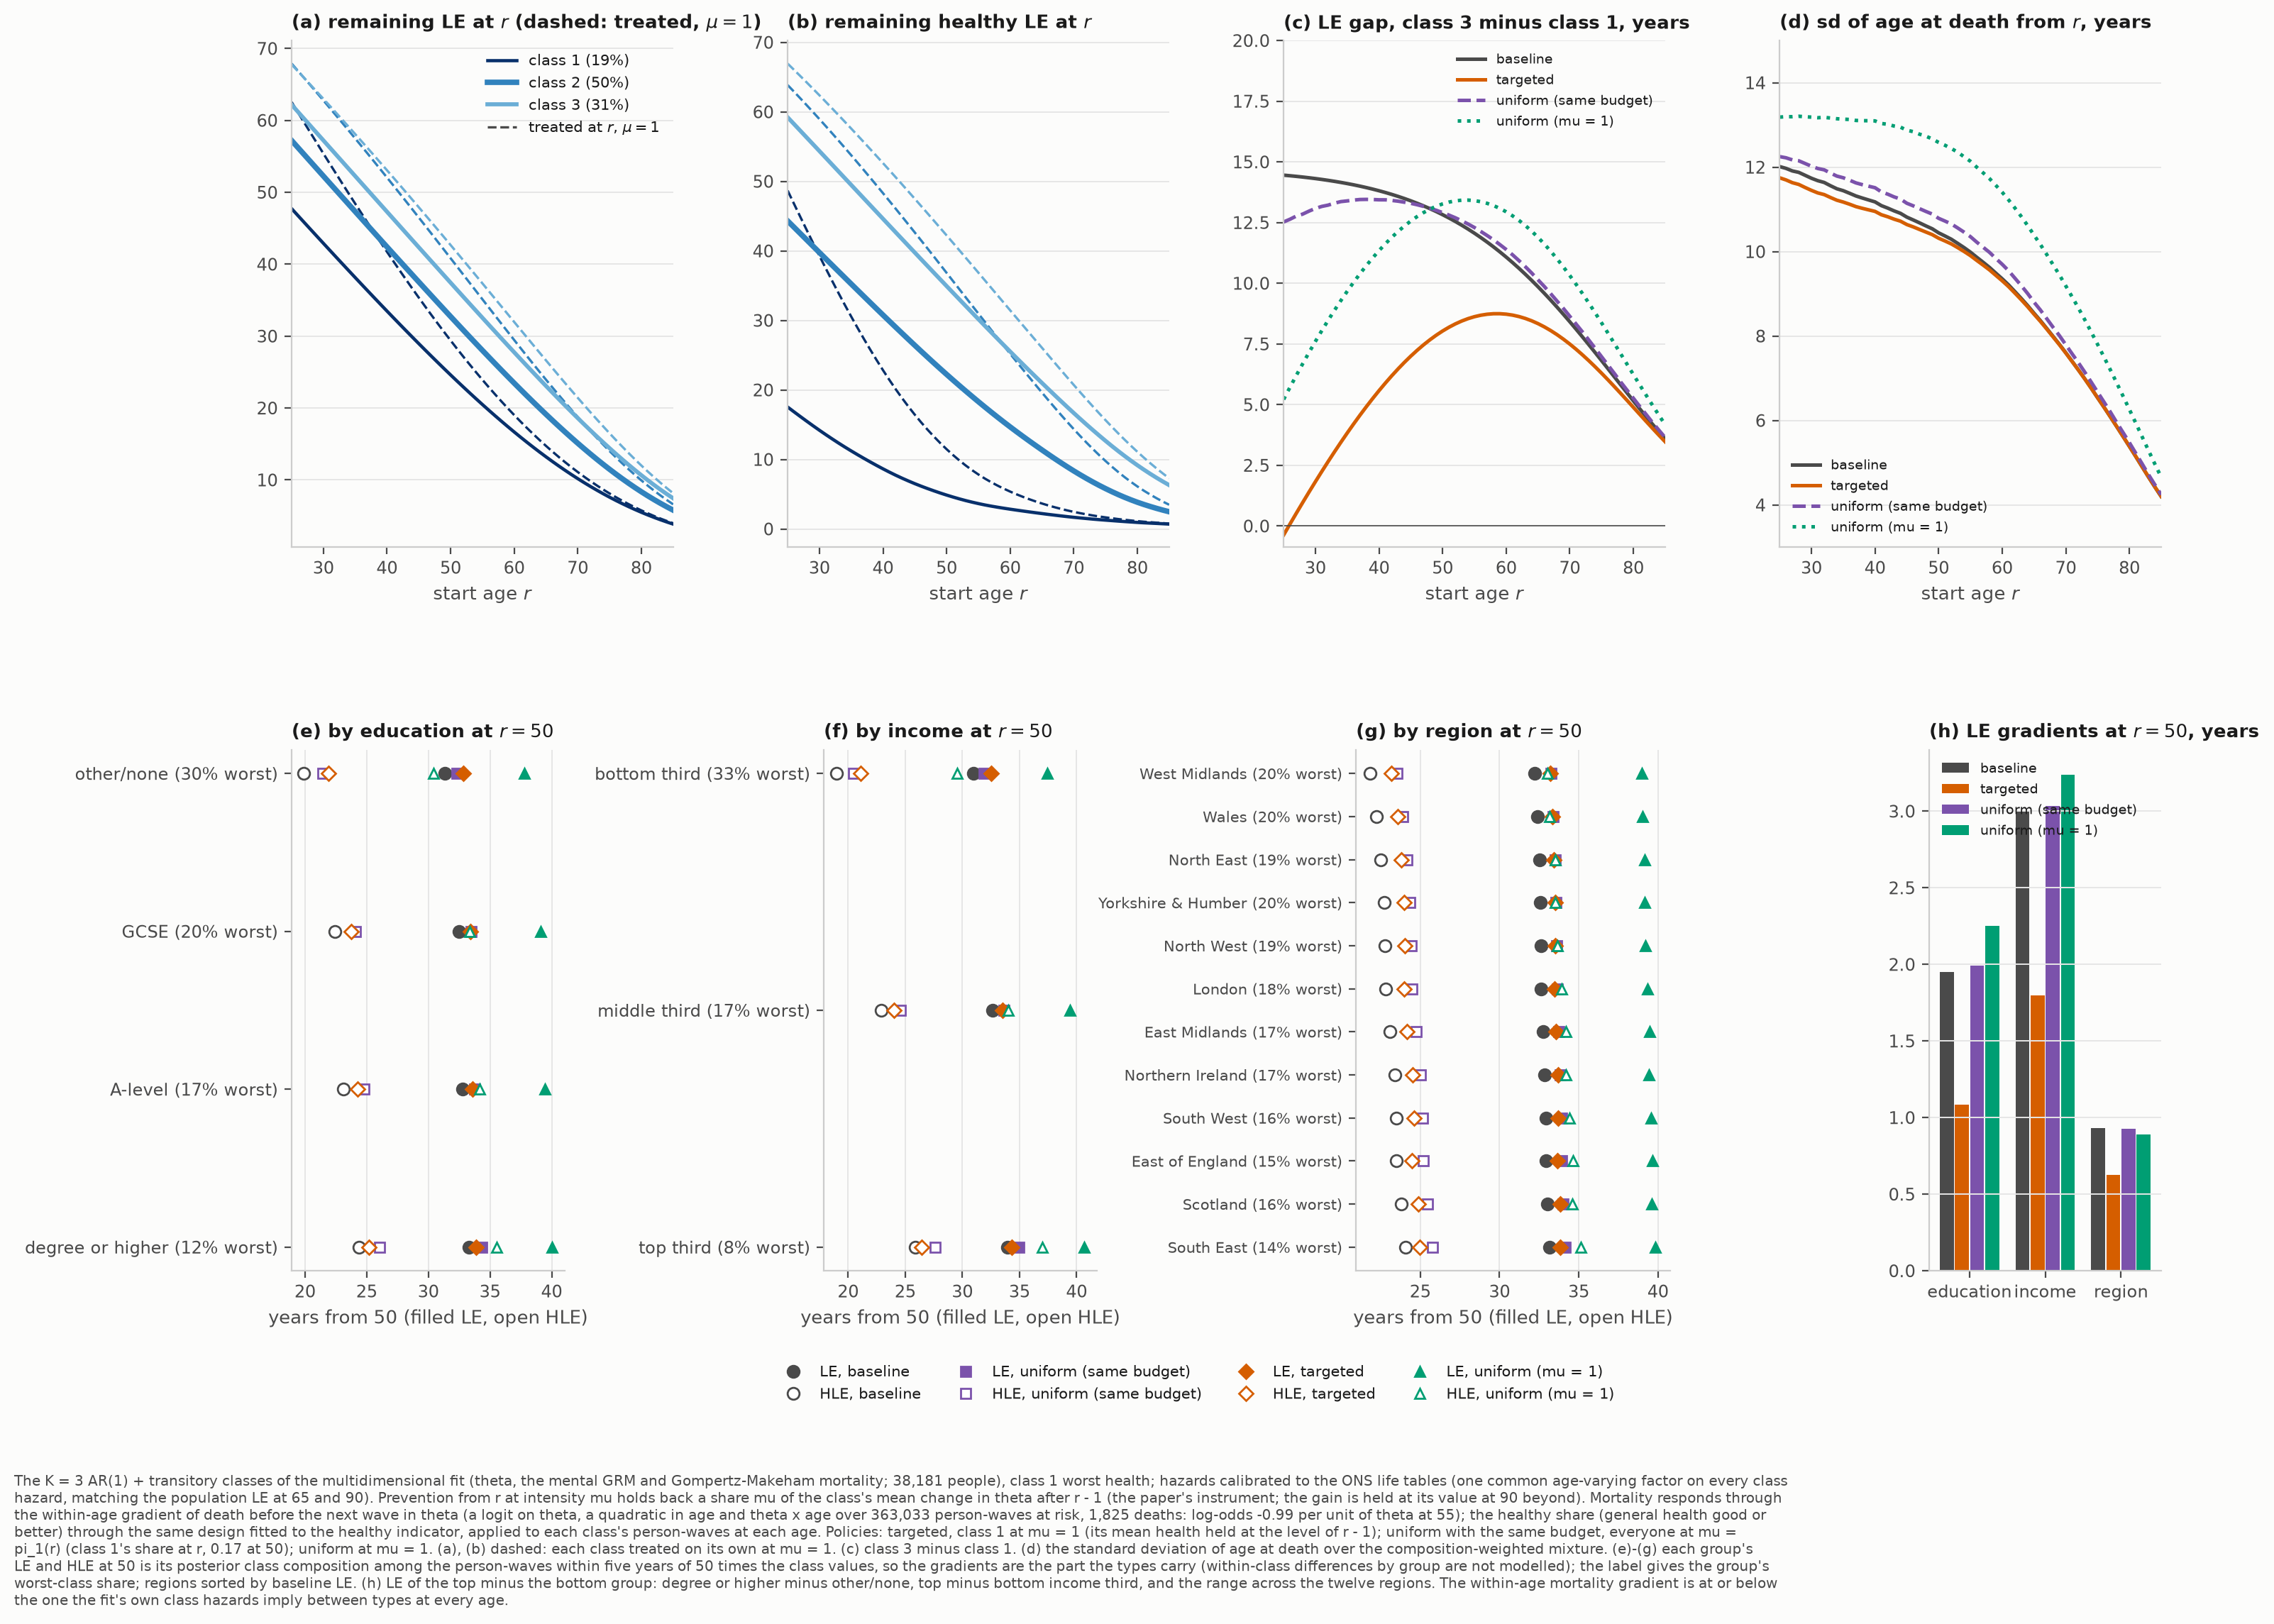
\includegraphics[width=\linewidth]{fig_prevention_le.png}
	\caption{As Figure~\ref{fig:prevle_uni}, on the multidimensional classes.}
	\label{fig:prevle_md}
\end{figure}
\begin{figure}[H]\centering
	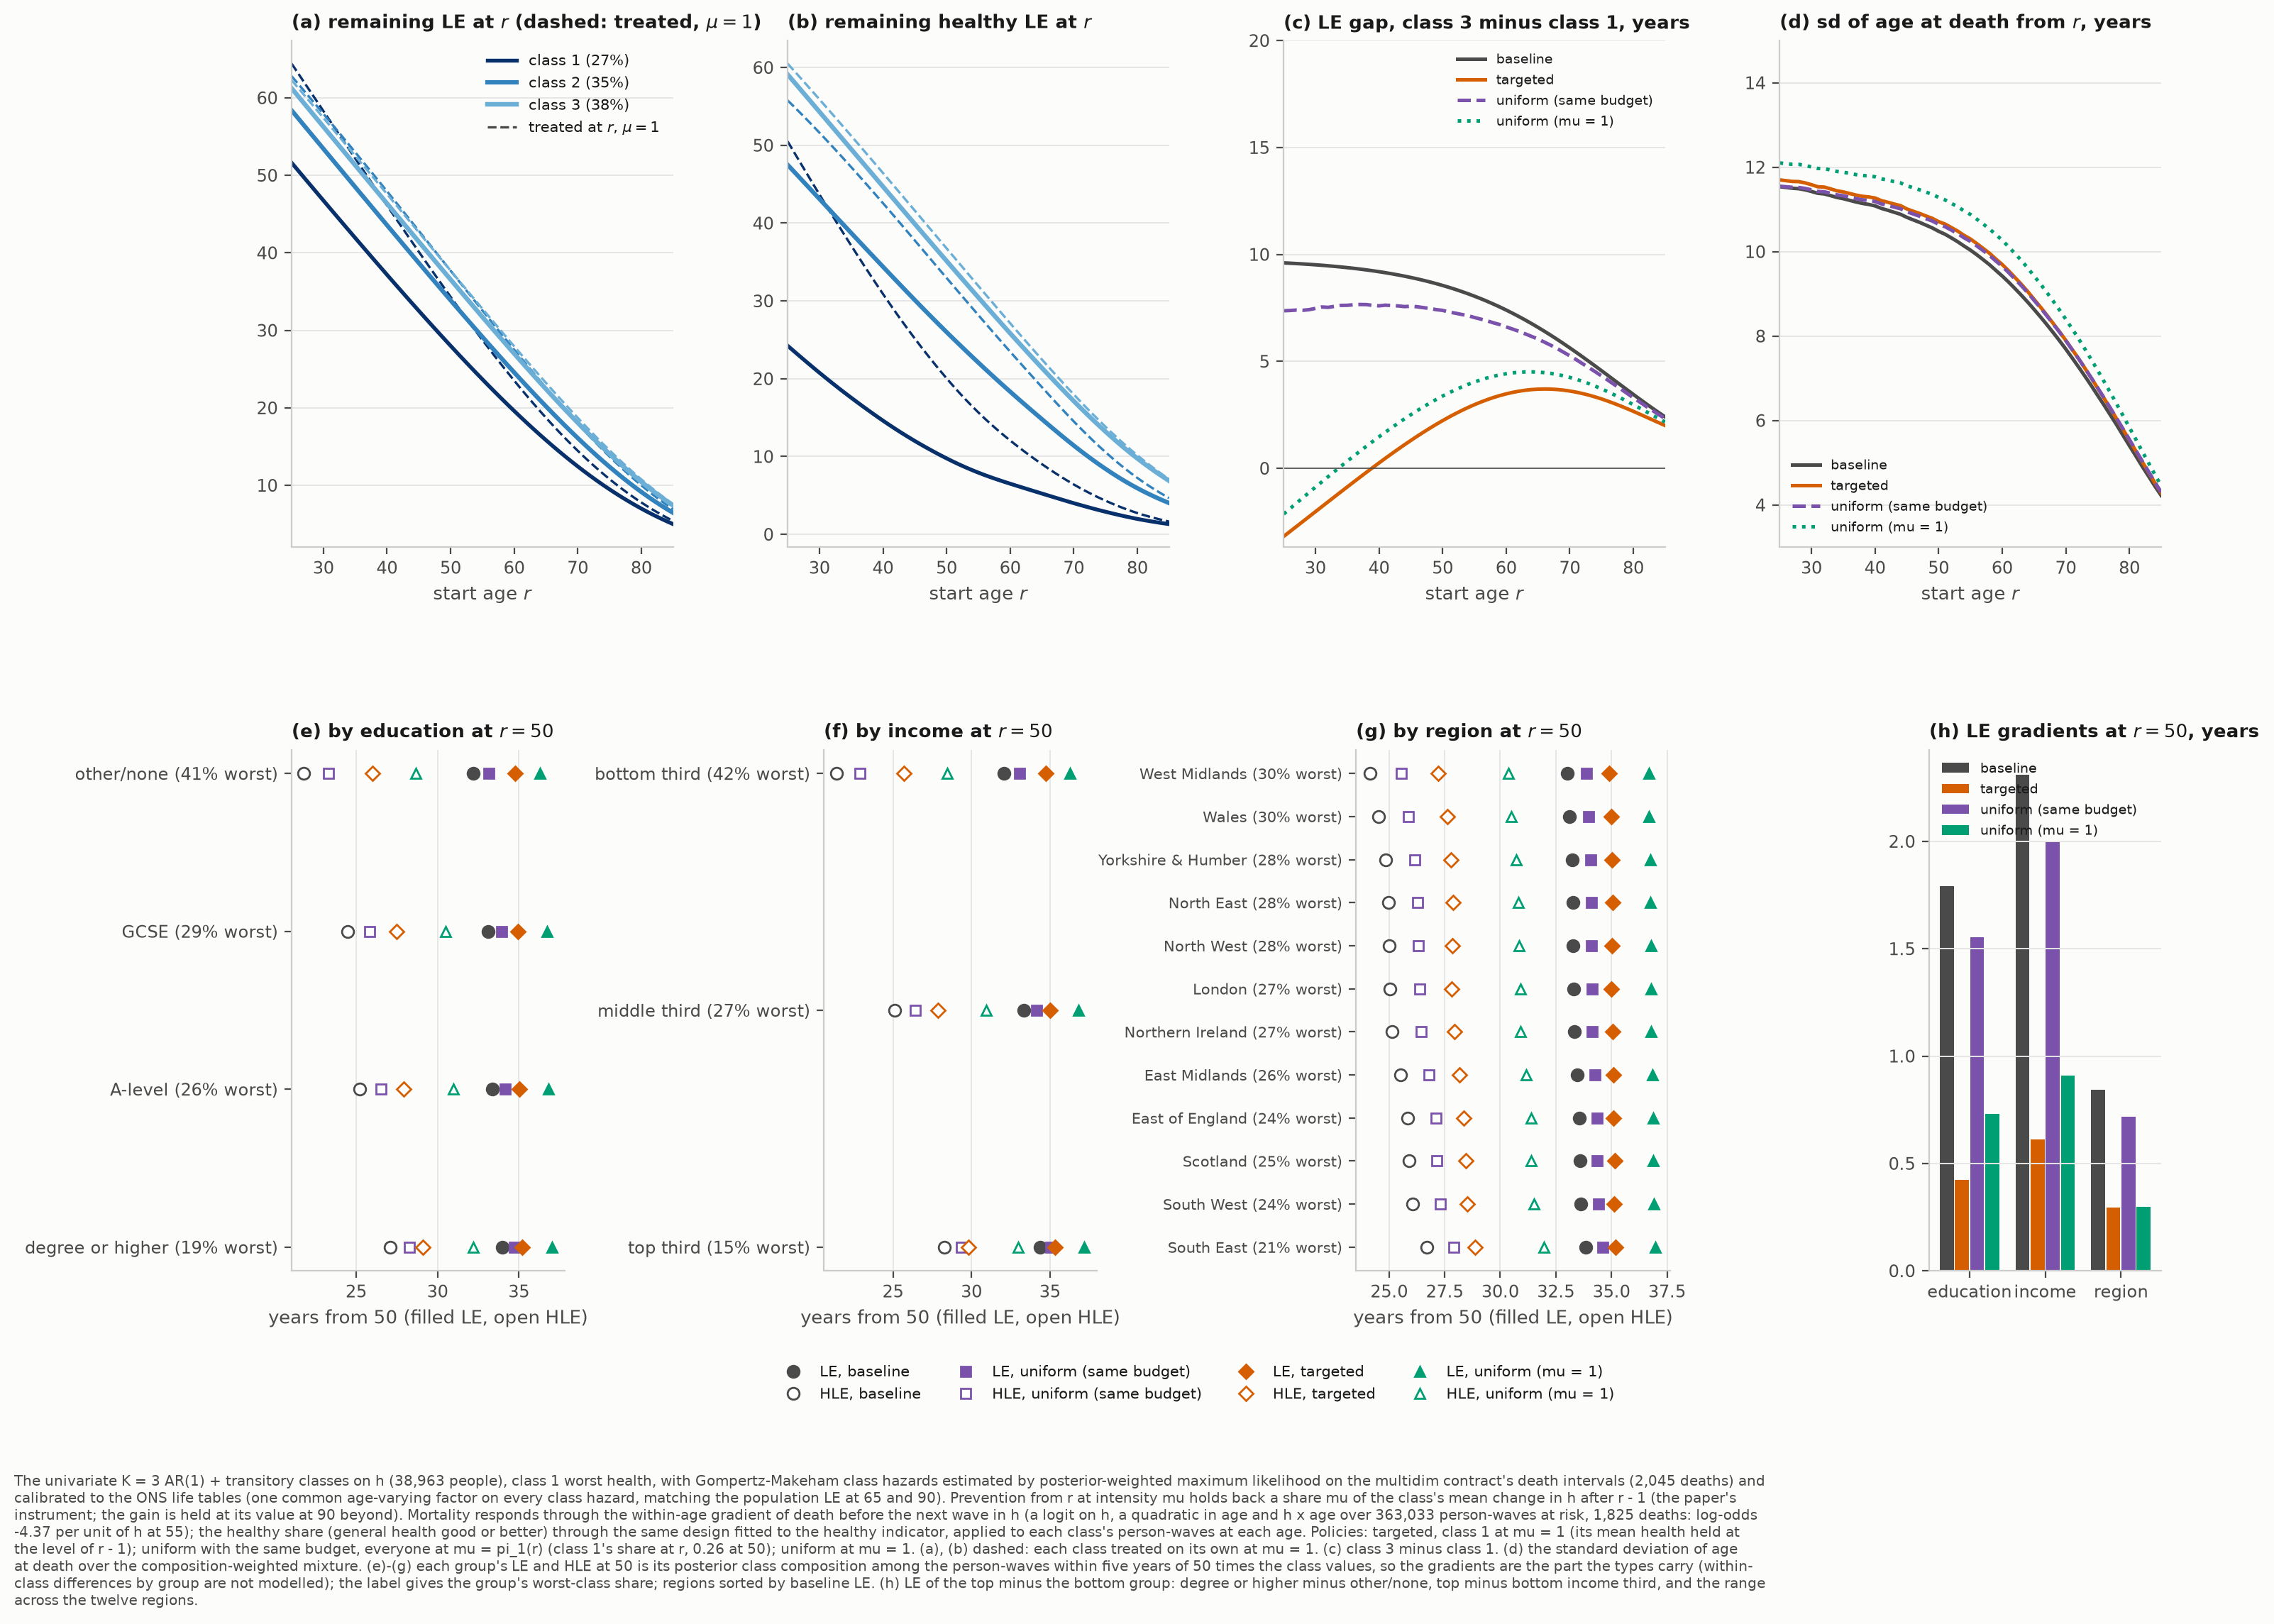
\includegraphics[width=\linewidth]{fig_prevention_le_h.png}
	\caption{As Figure~\ref{fig:prevle_uni}, on $h$.}
	\label{fig:prevle_h}
\end{figure}
\begin{figure}[H]\centering
	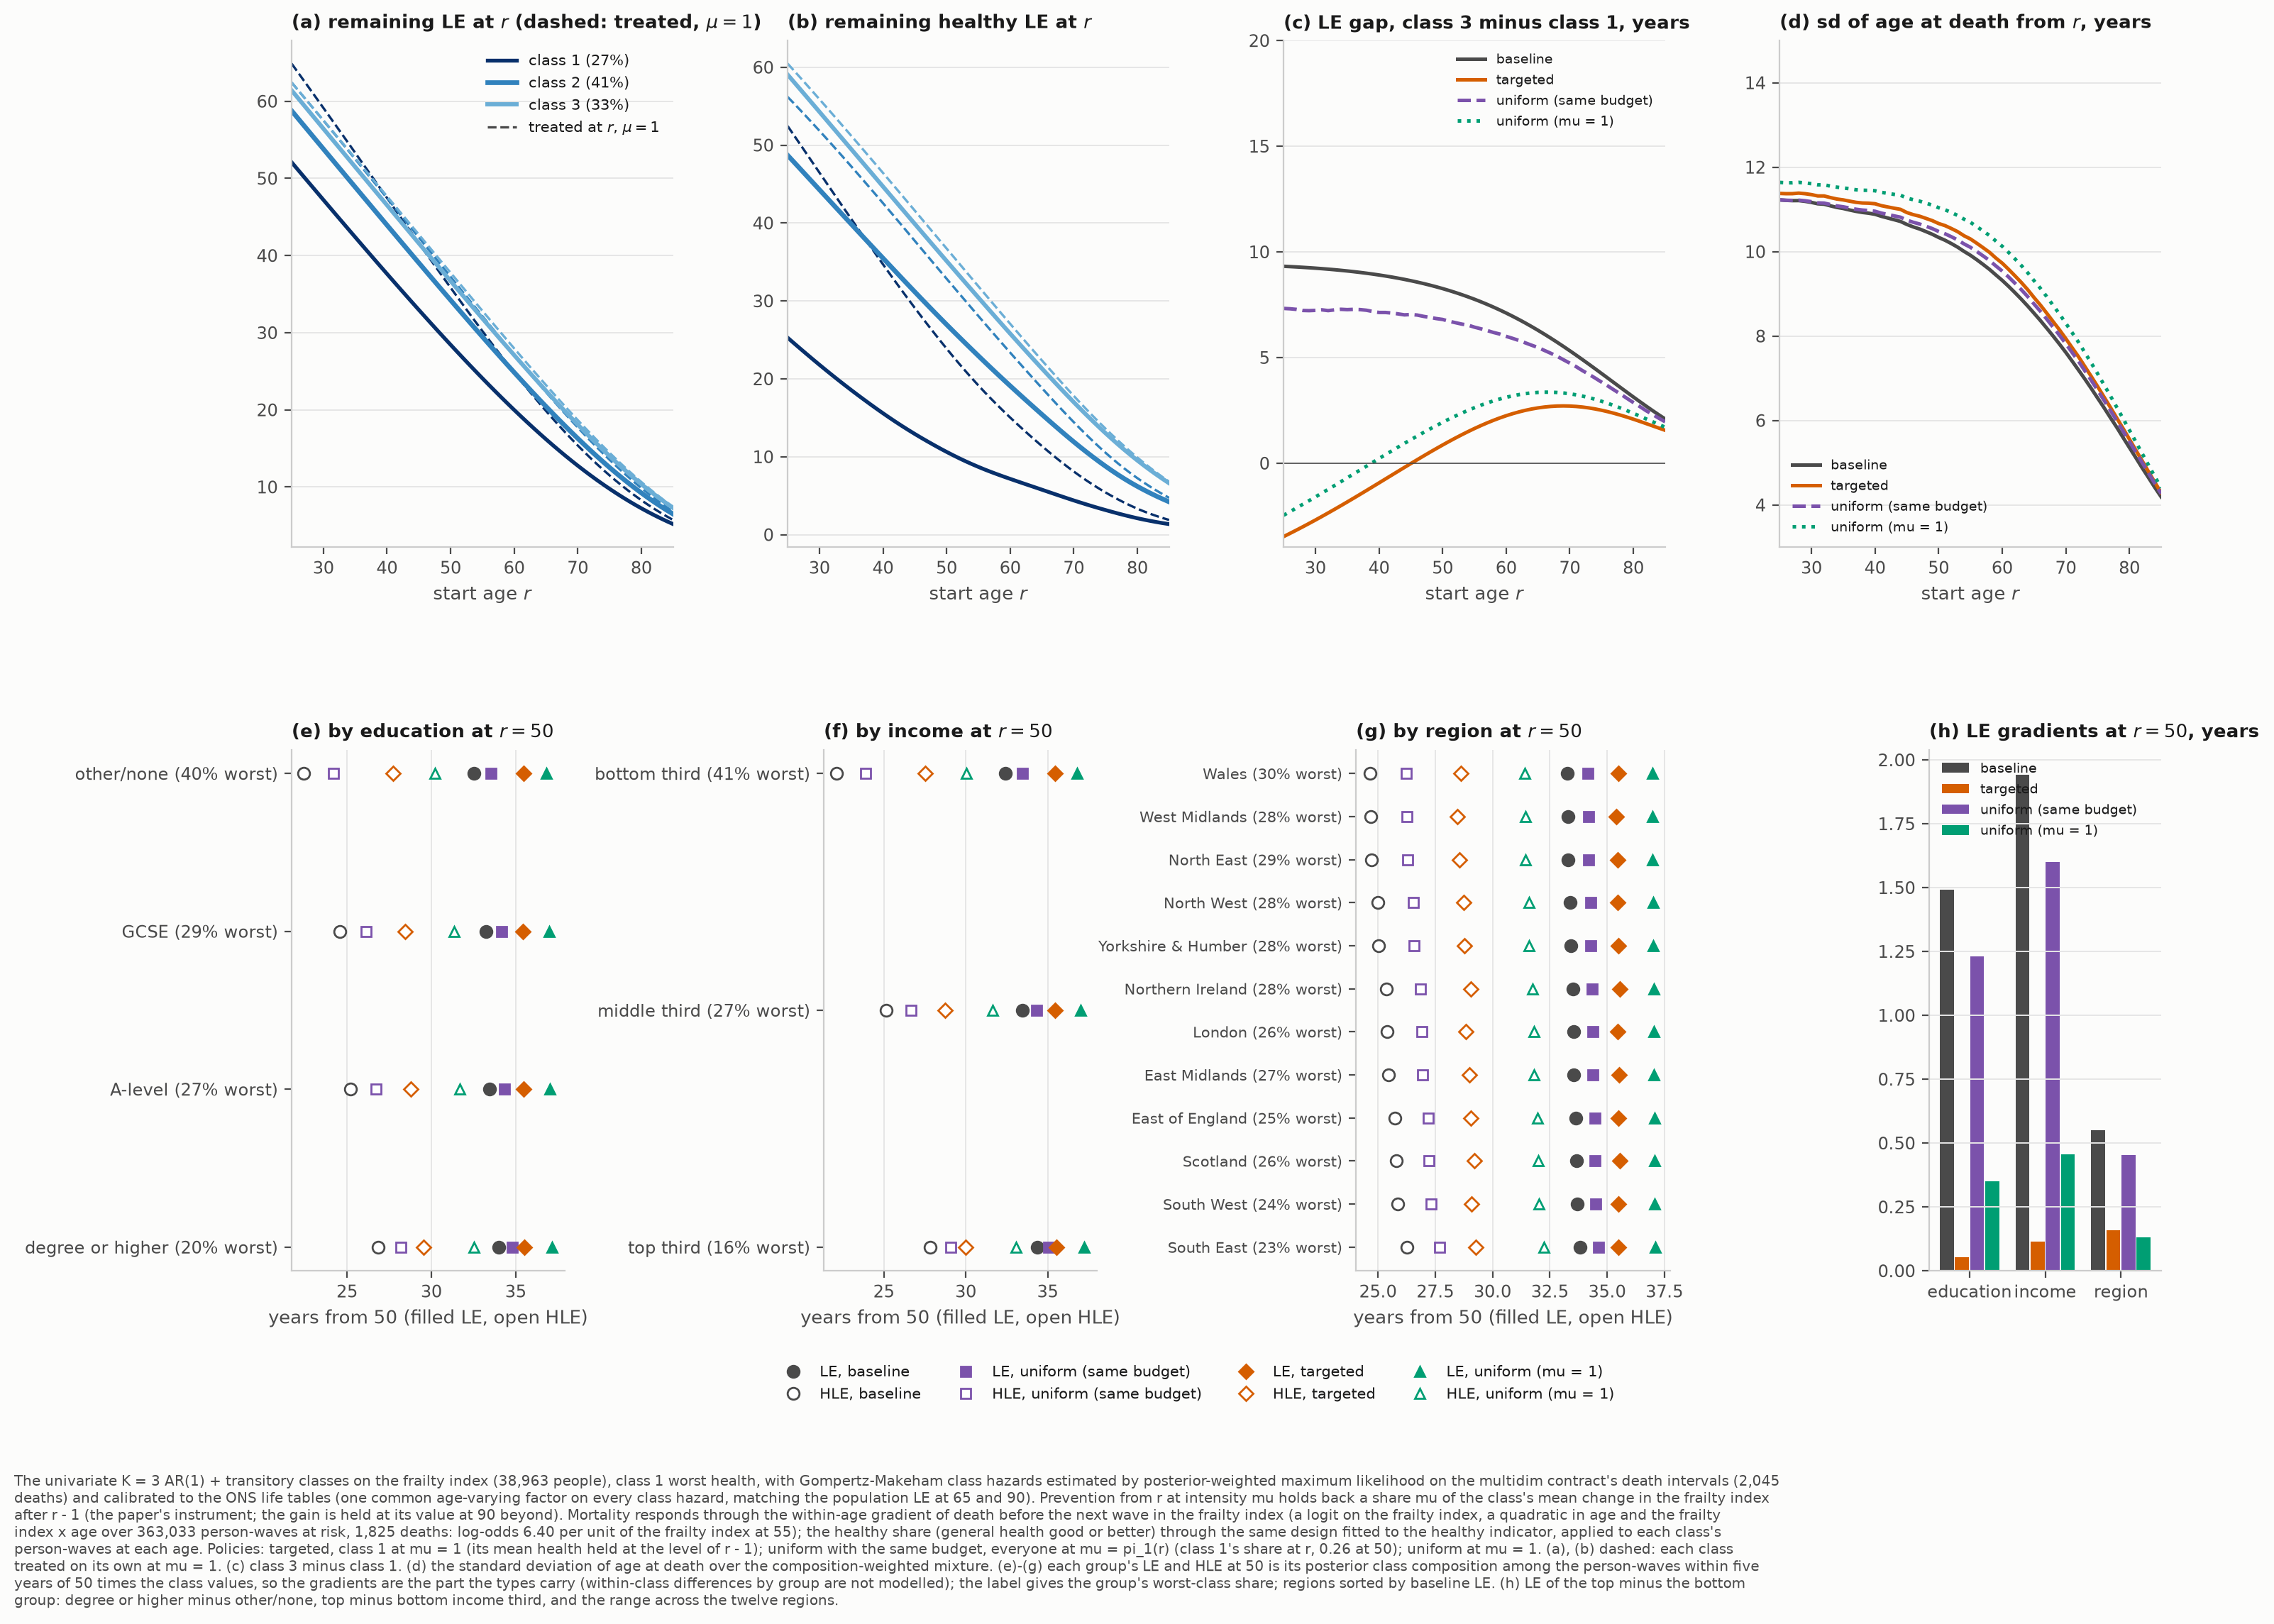
\includegraphics[width=\linewidth]{fig_prevention_le_frailty.png}
	\caption{As Figure~\ref{fig:prevle_uni}, on the frailty index.}
	\label{fig:prevle_frailty}
\end{figure}
\begin{figure}[H]\centering
	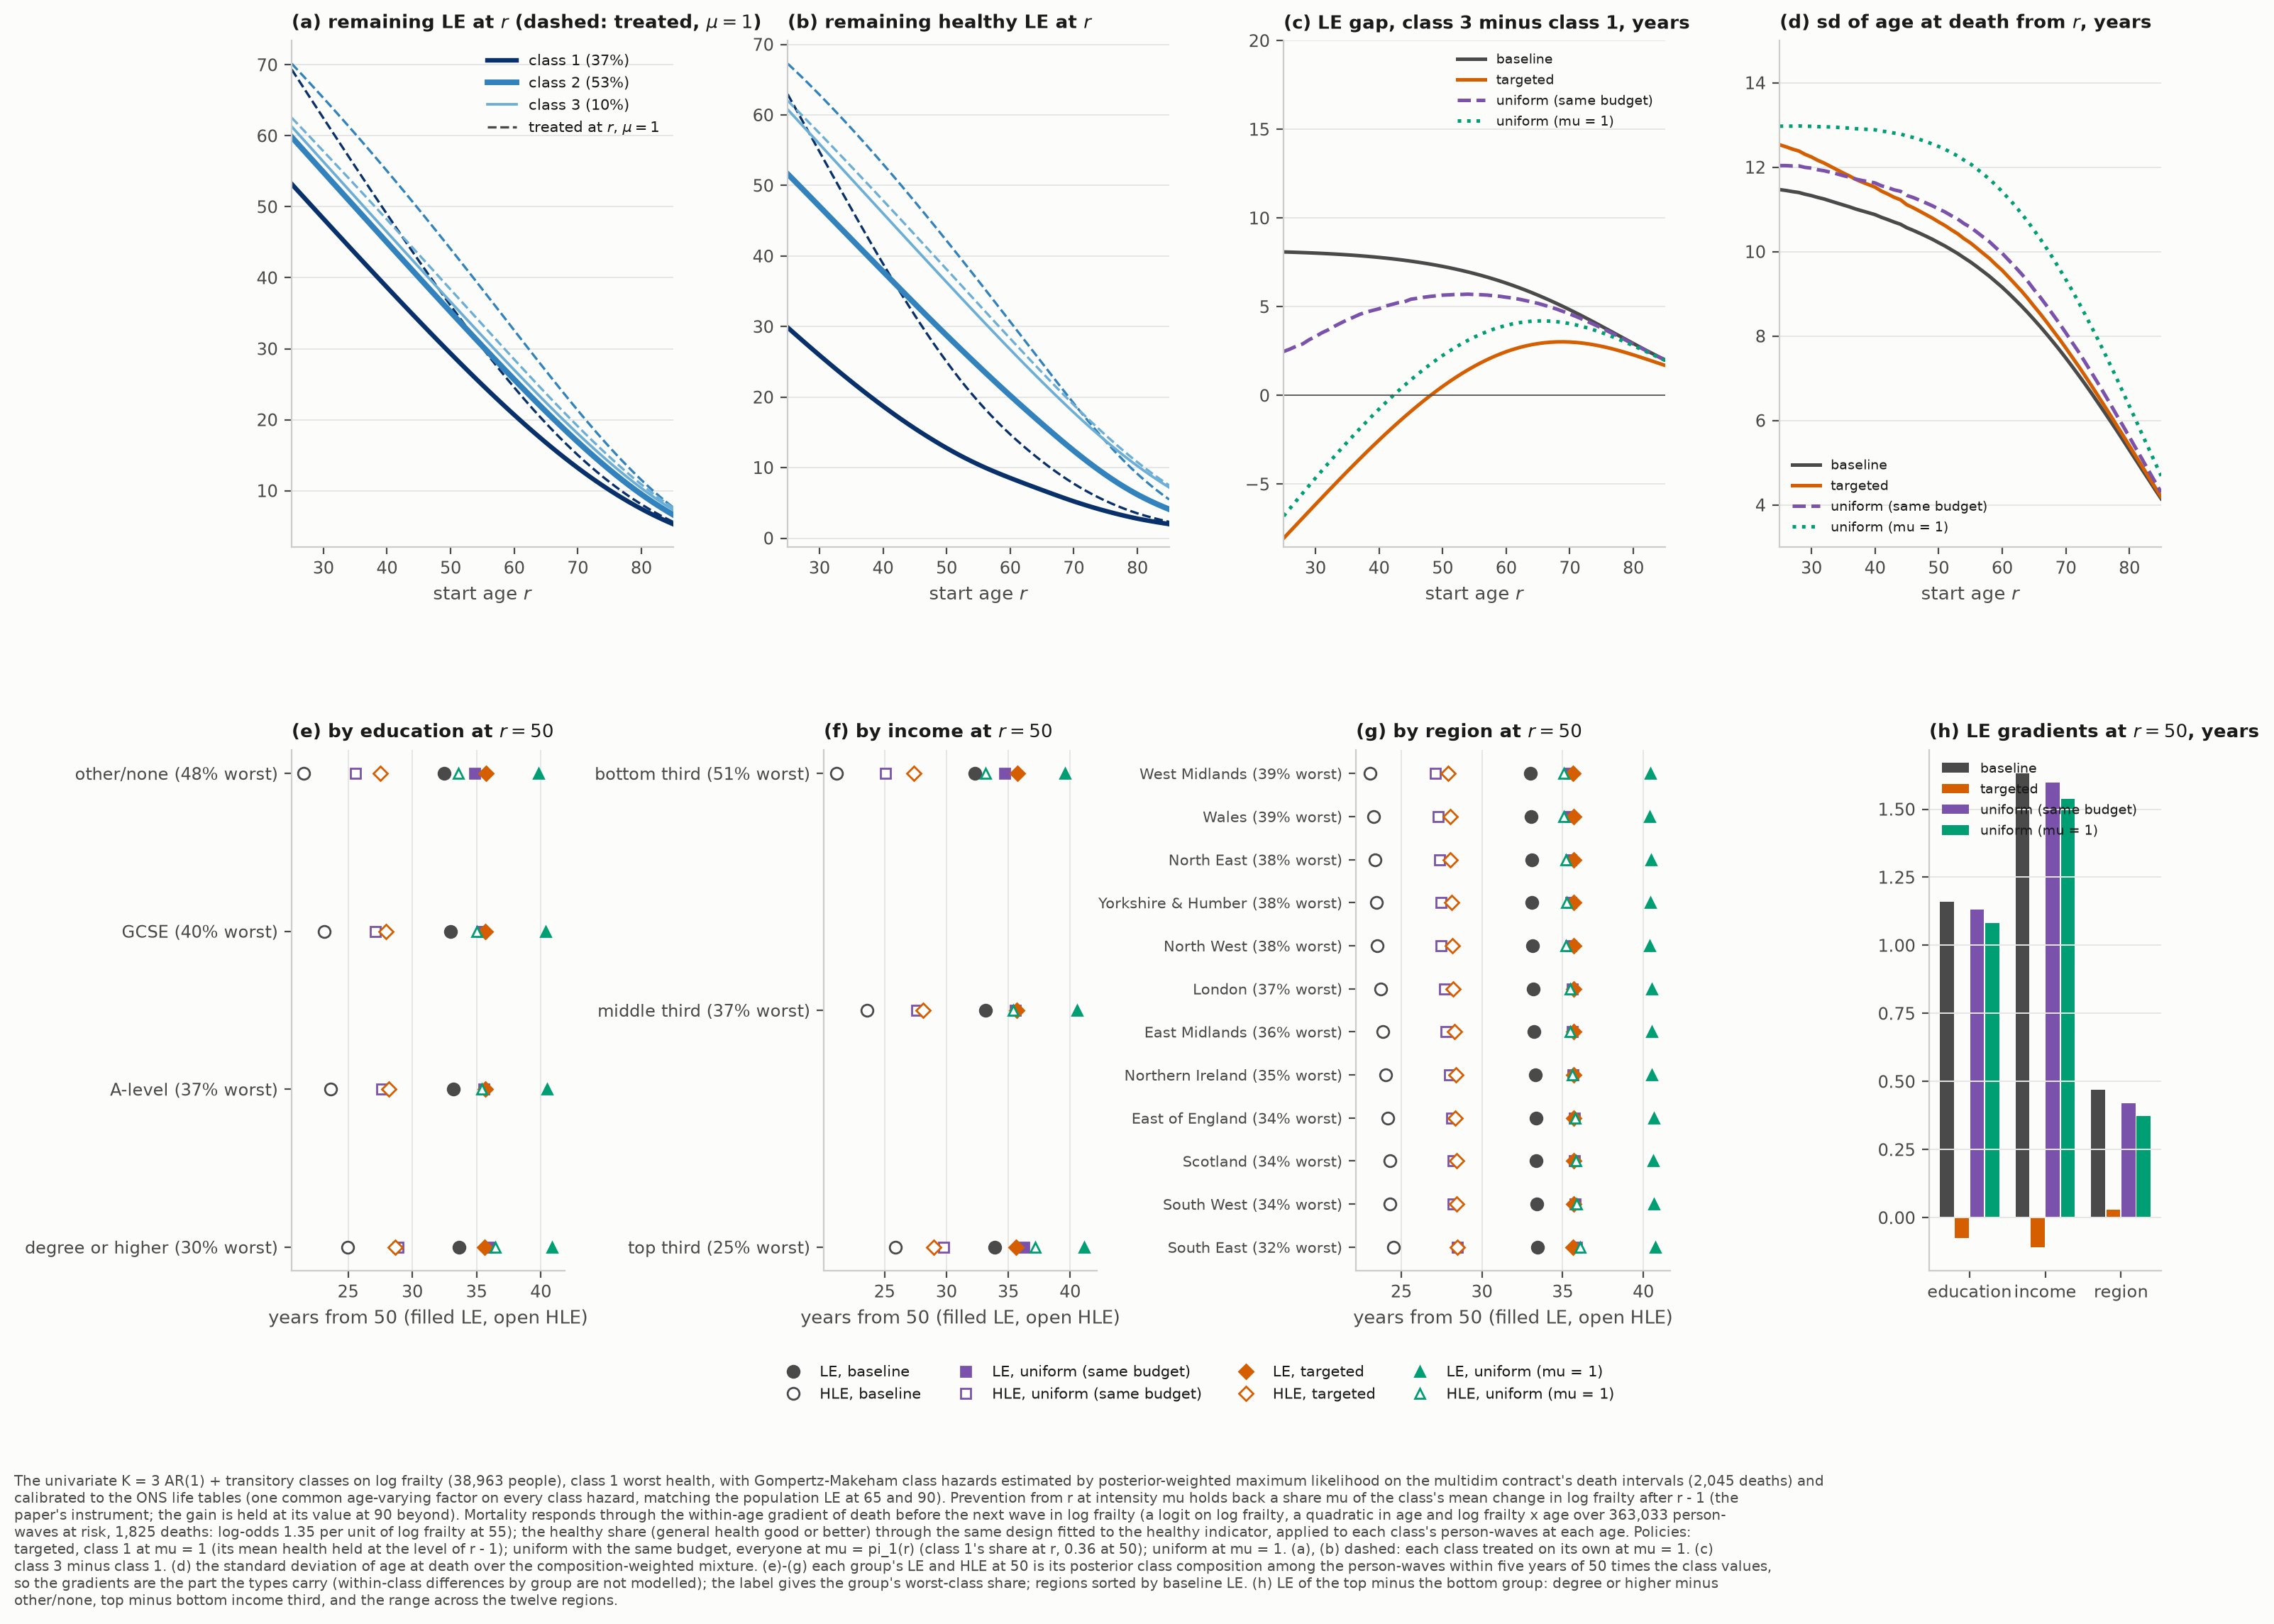
\includegraphics[width=\linewidth]{fig_prevention_le_logfrailty.png}
	\caption{As Figure~\ref{fig:prevle_uni}, on log frailty.}
	\label{fig:prevle_logfrailty}
\end{figure}

\section{Mental Health} \label{app:mental}
\begin{itemize}
	\item Half the variance is one-period noise; the mixtures then sort by persistence, not level, so mental health cannot carry its own level typology.
	\item Cost and mortality gradients are weaker than on $\theta$.
\end{itemize}
\begin{figure}[H]\centering
	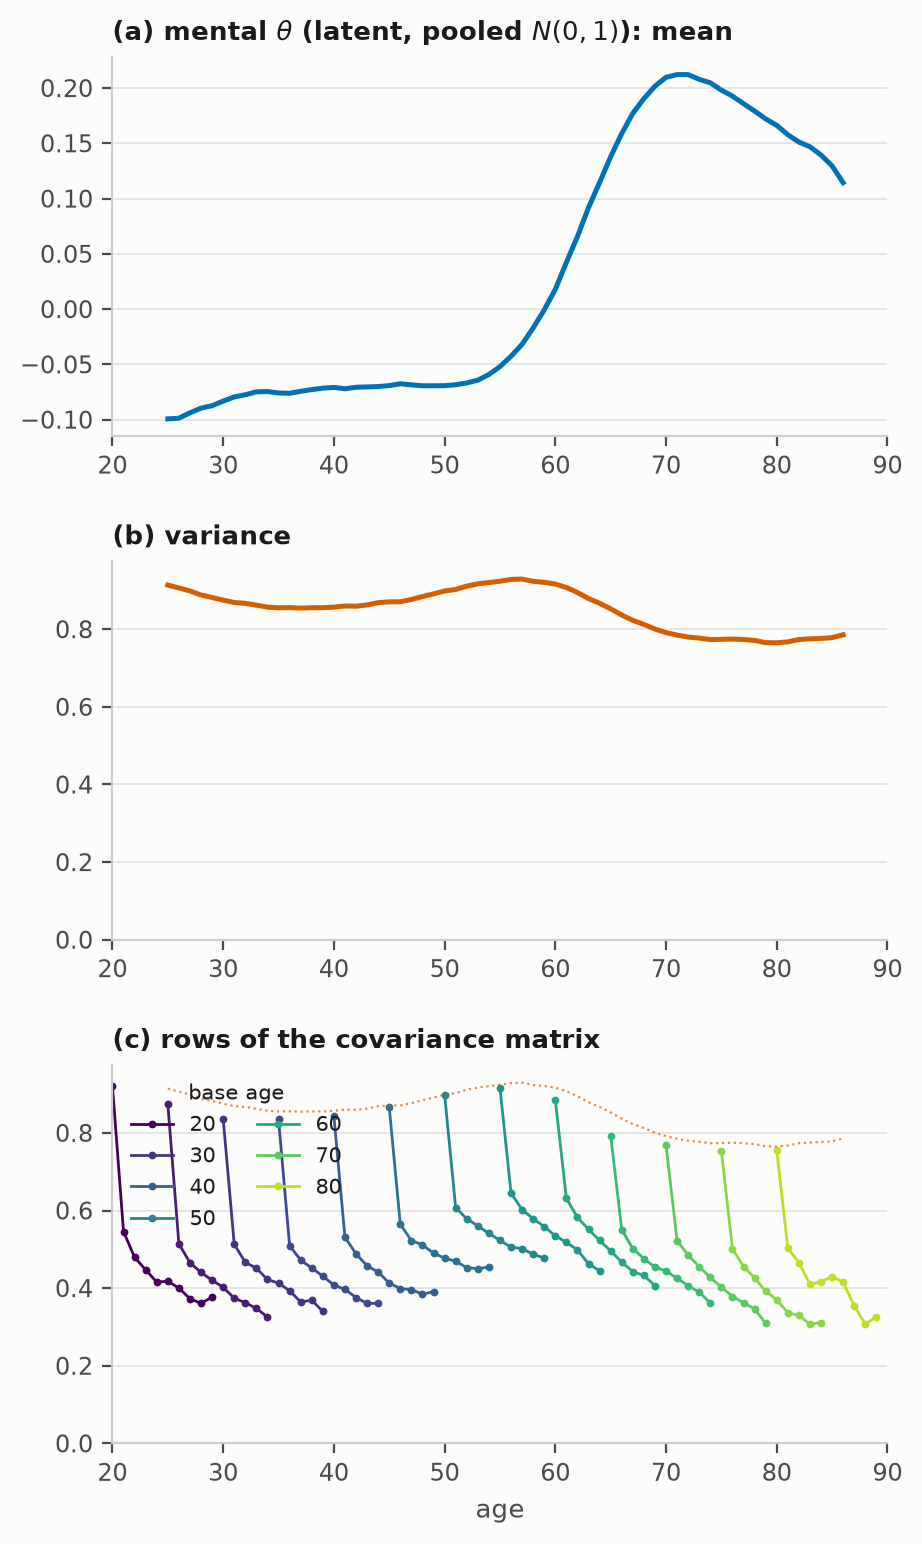
\includegraphics[width=0.45\linewidth]{fig_exhibit1_mental.png}
	\caption{As Figure~\ref{fig:exhibit1}, on the mental GRM.}
	\label{fig:exhibit1_mental}
\end{figure}
\begin{figure}[H]\centering
	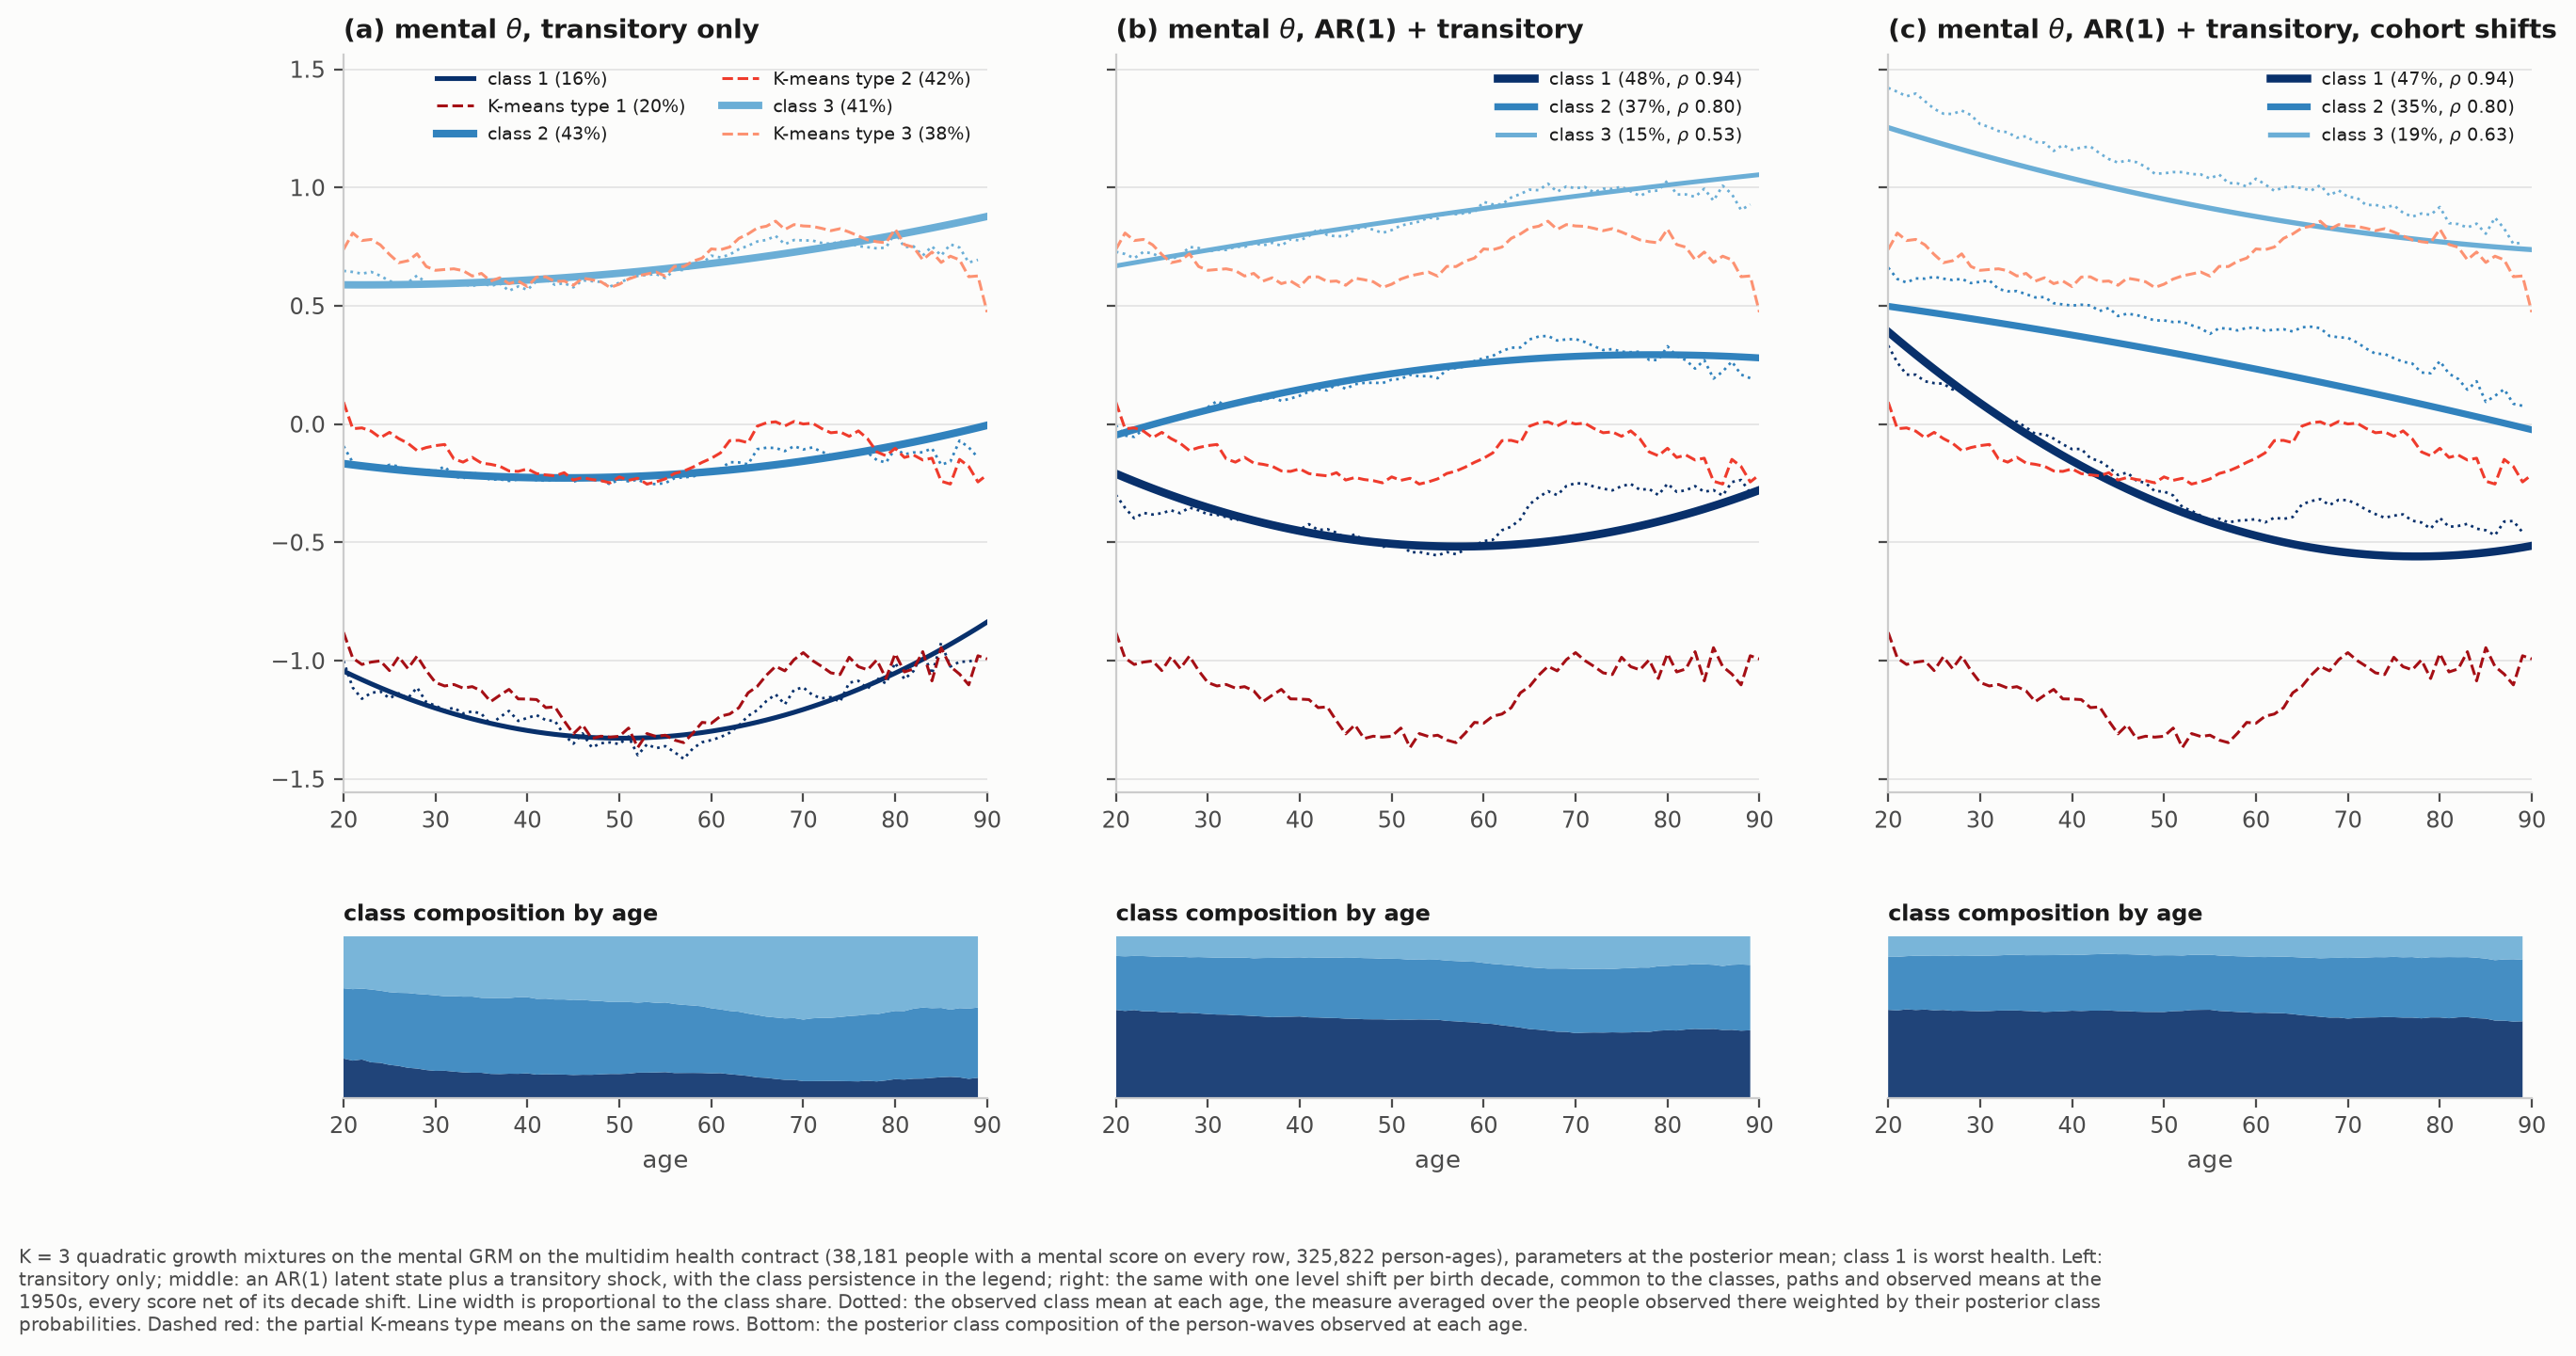
\includegraphics[width=\linewidth]{fig_bayes_mixtures_mental.png}
	\caption{$K=3$ mixtures on the mental GRM.}
	\label{fig:bayes_mental}
\end{figure}

\section{The Main Figures on the Other Measures} \label{app:measures}
\begin{figure}[H]\centering
	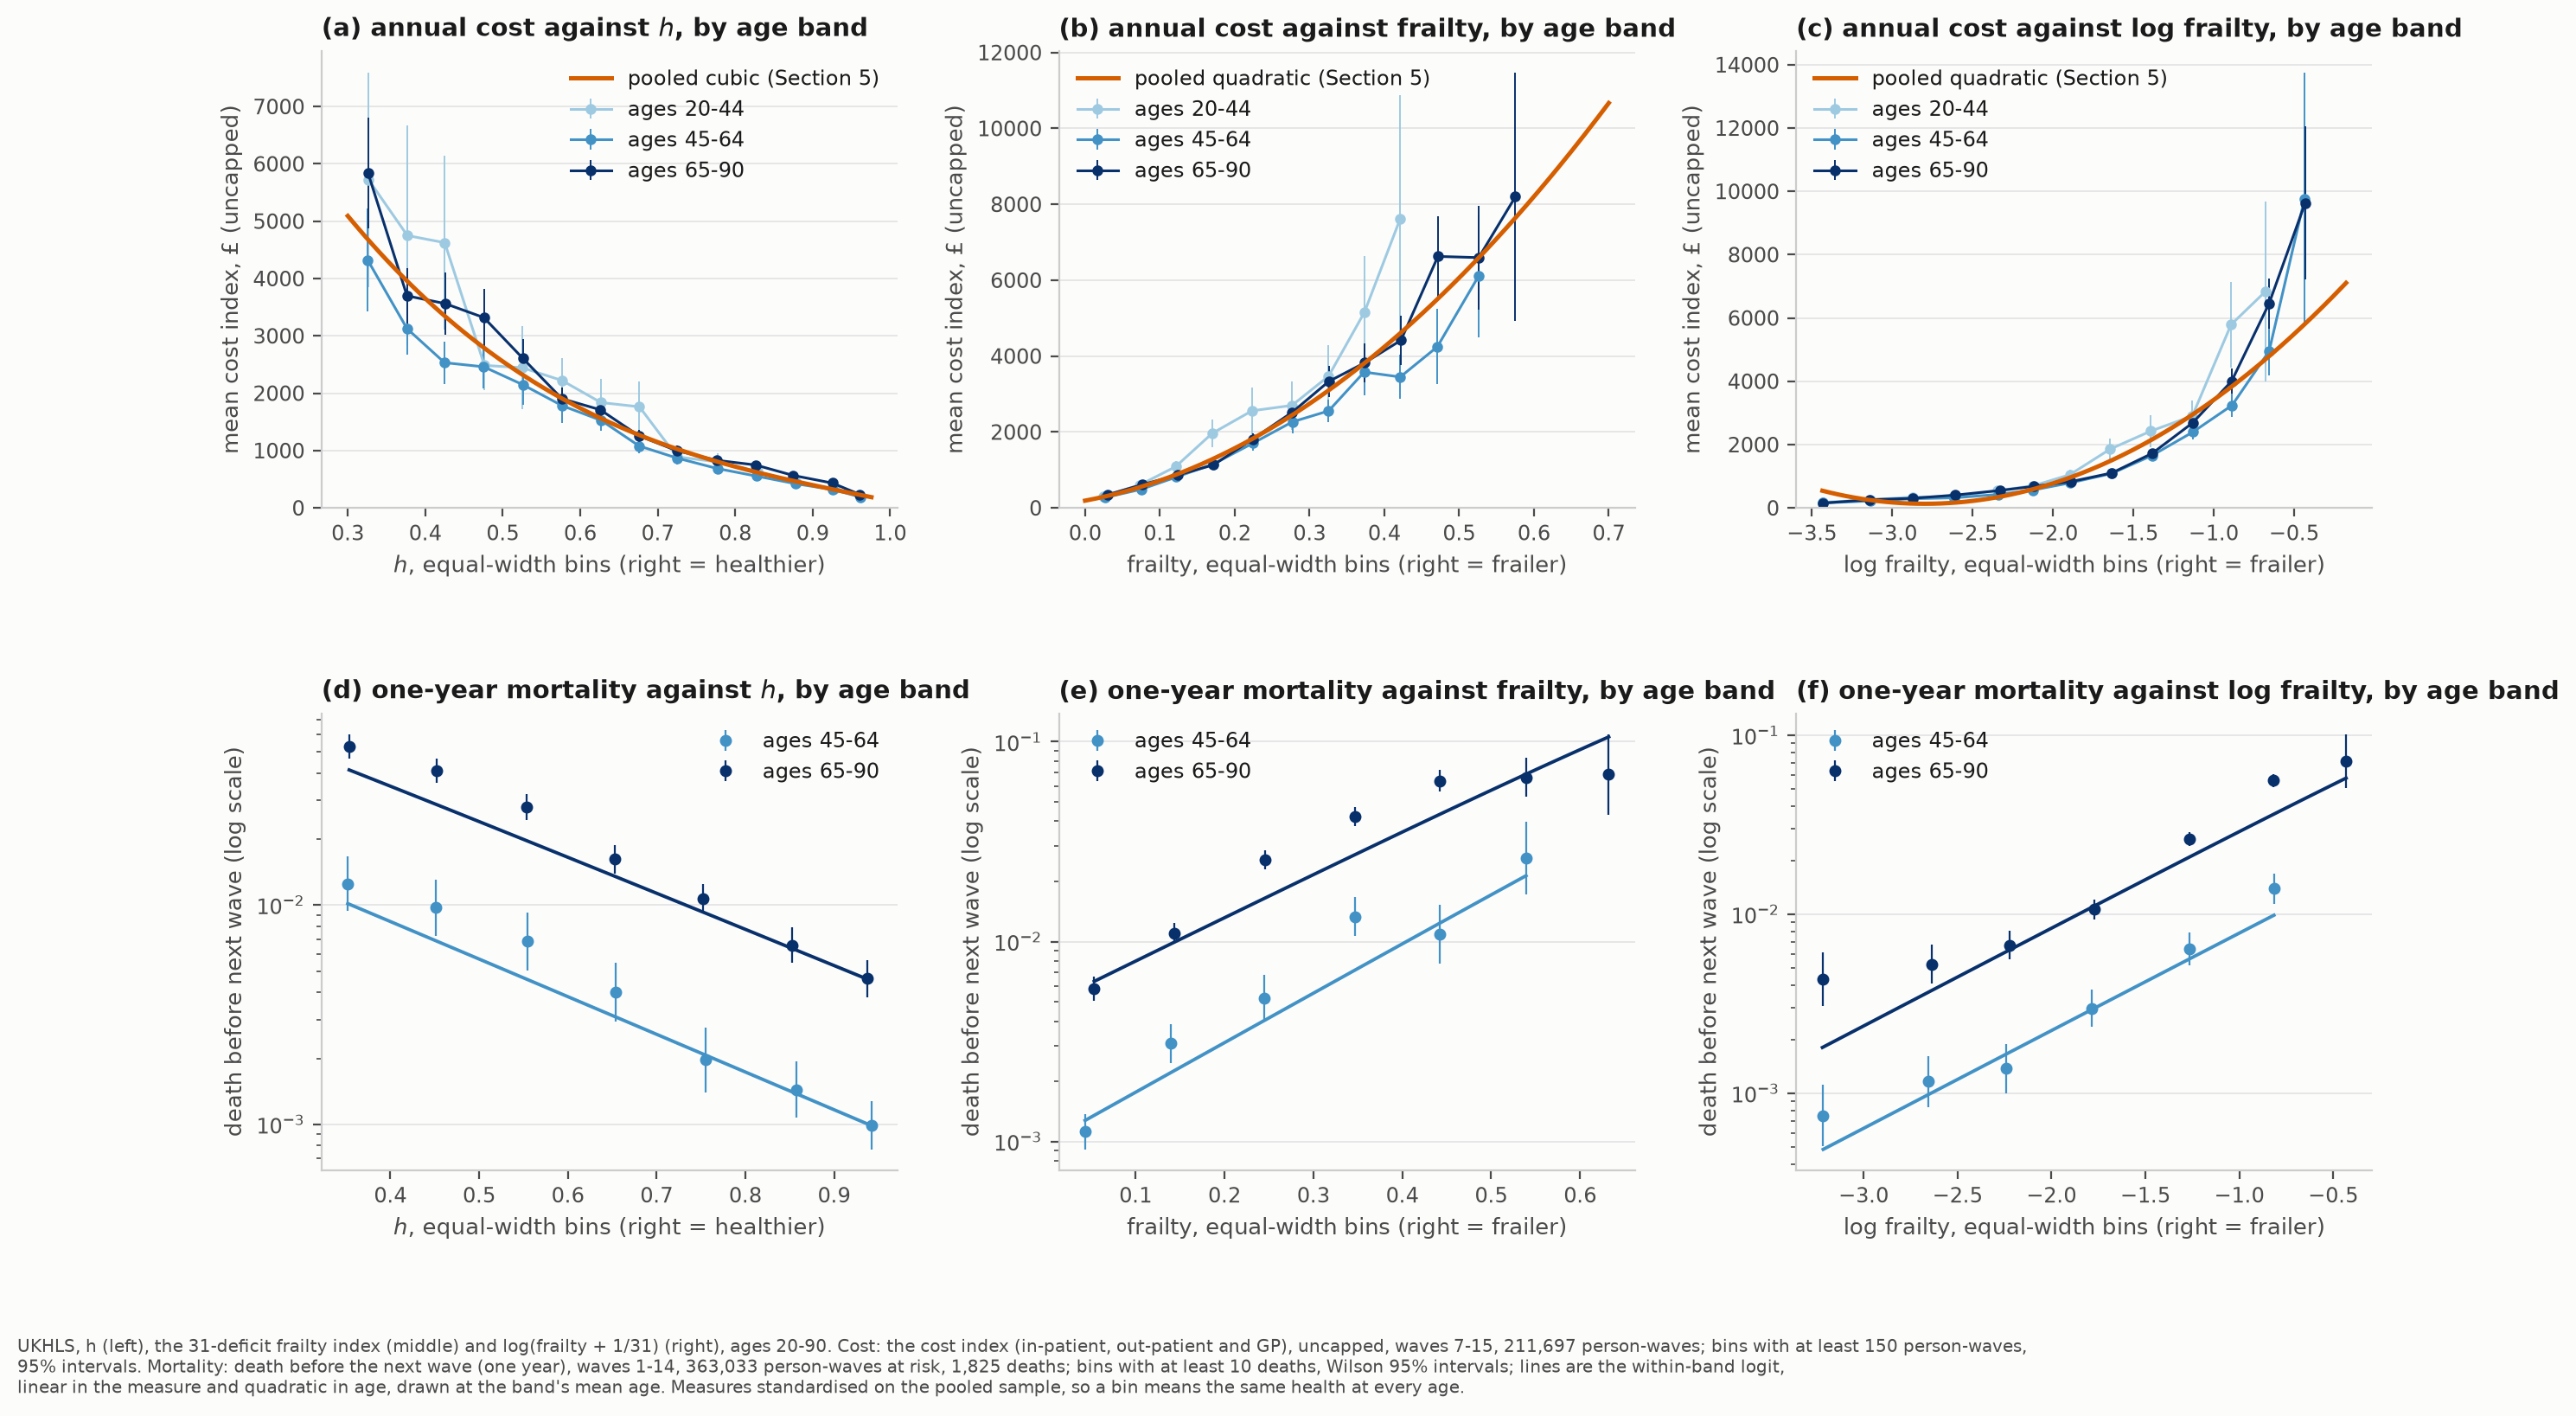
\includegraphics[width=\linewidth]{fig_cost_mortality_age_measures.png}
	\caption{As Figure~\ref{fig:cost}, on $h$, frailty and log frailty.}
	\label{fig:cost_measures}
\end{figure}
\begin{figure}[H]\centering
	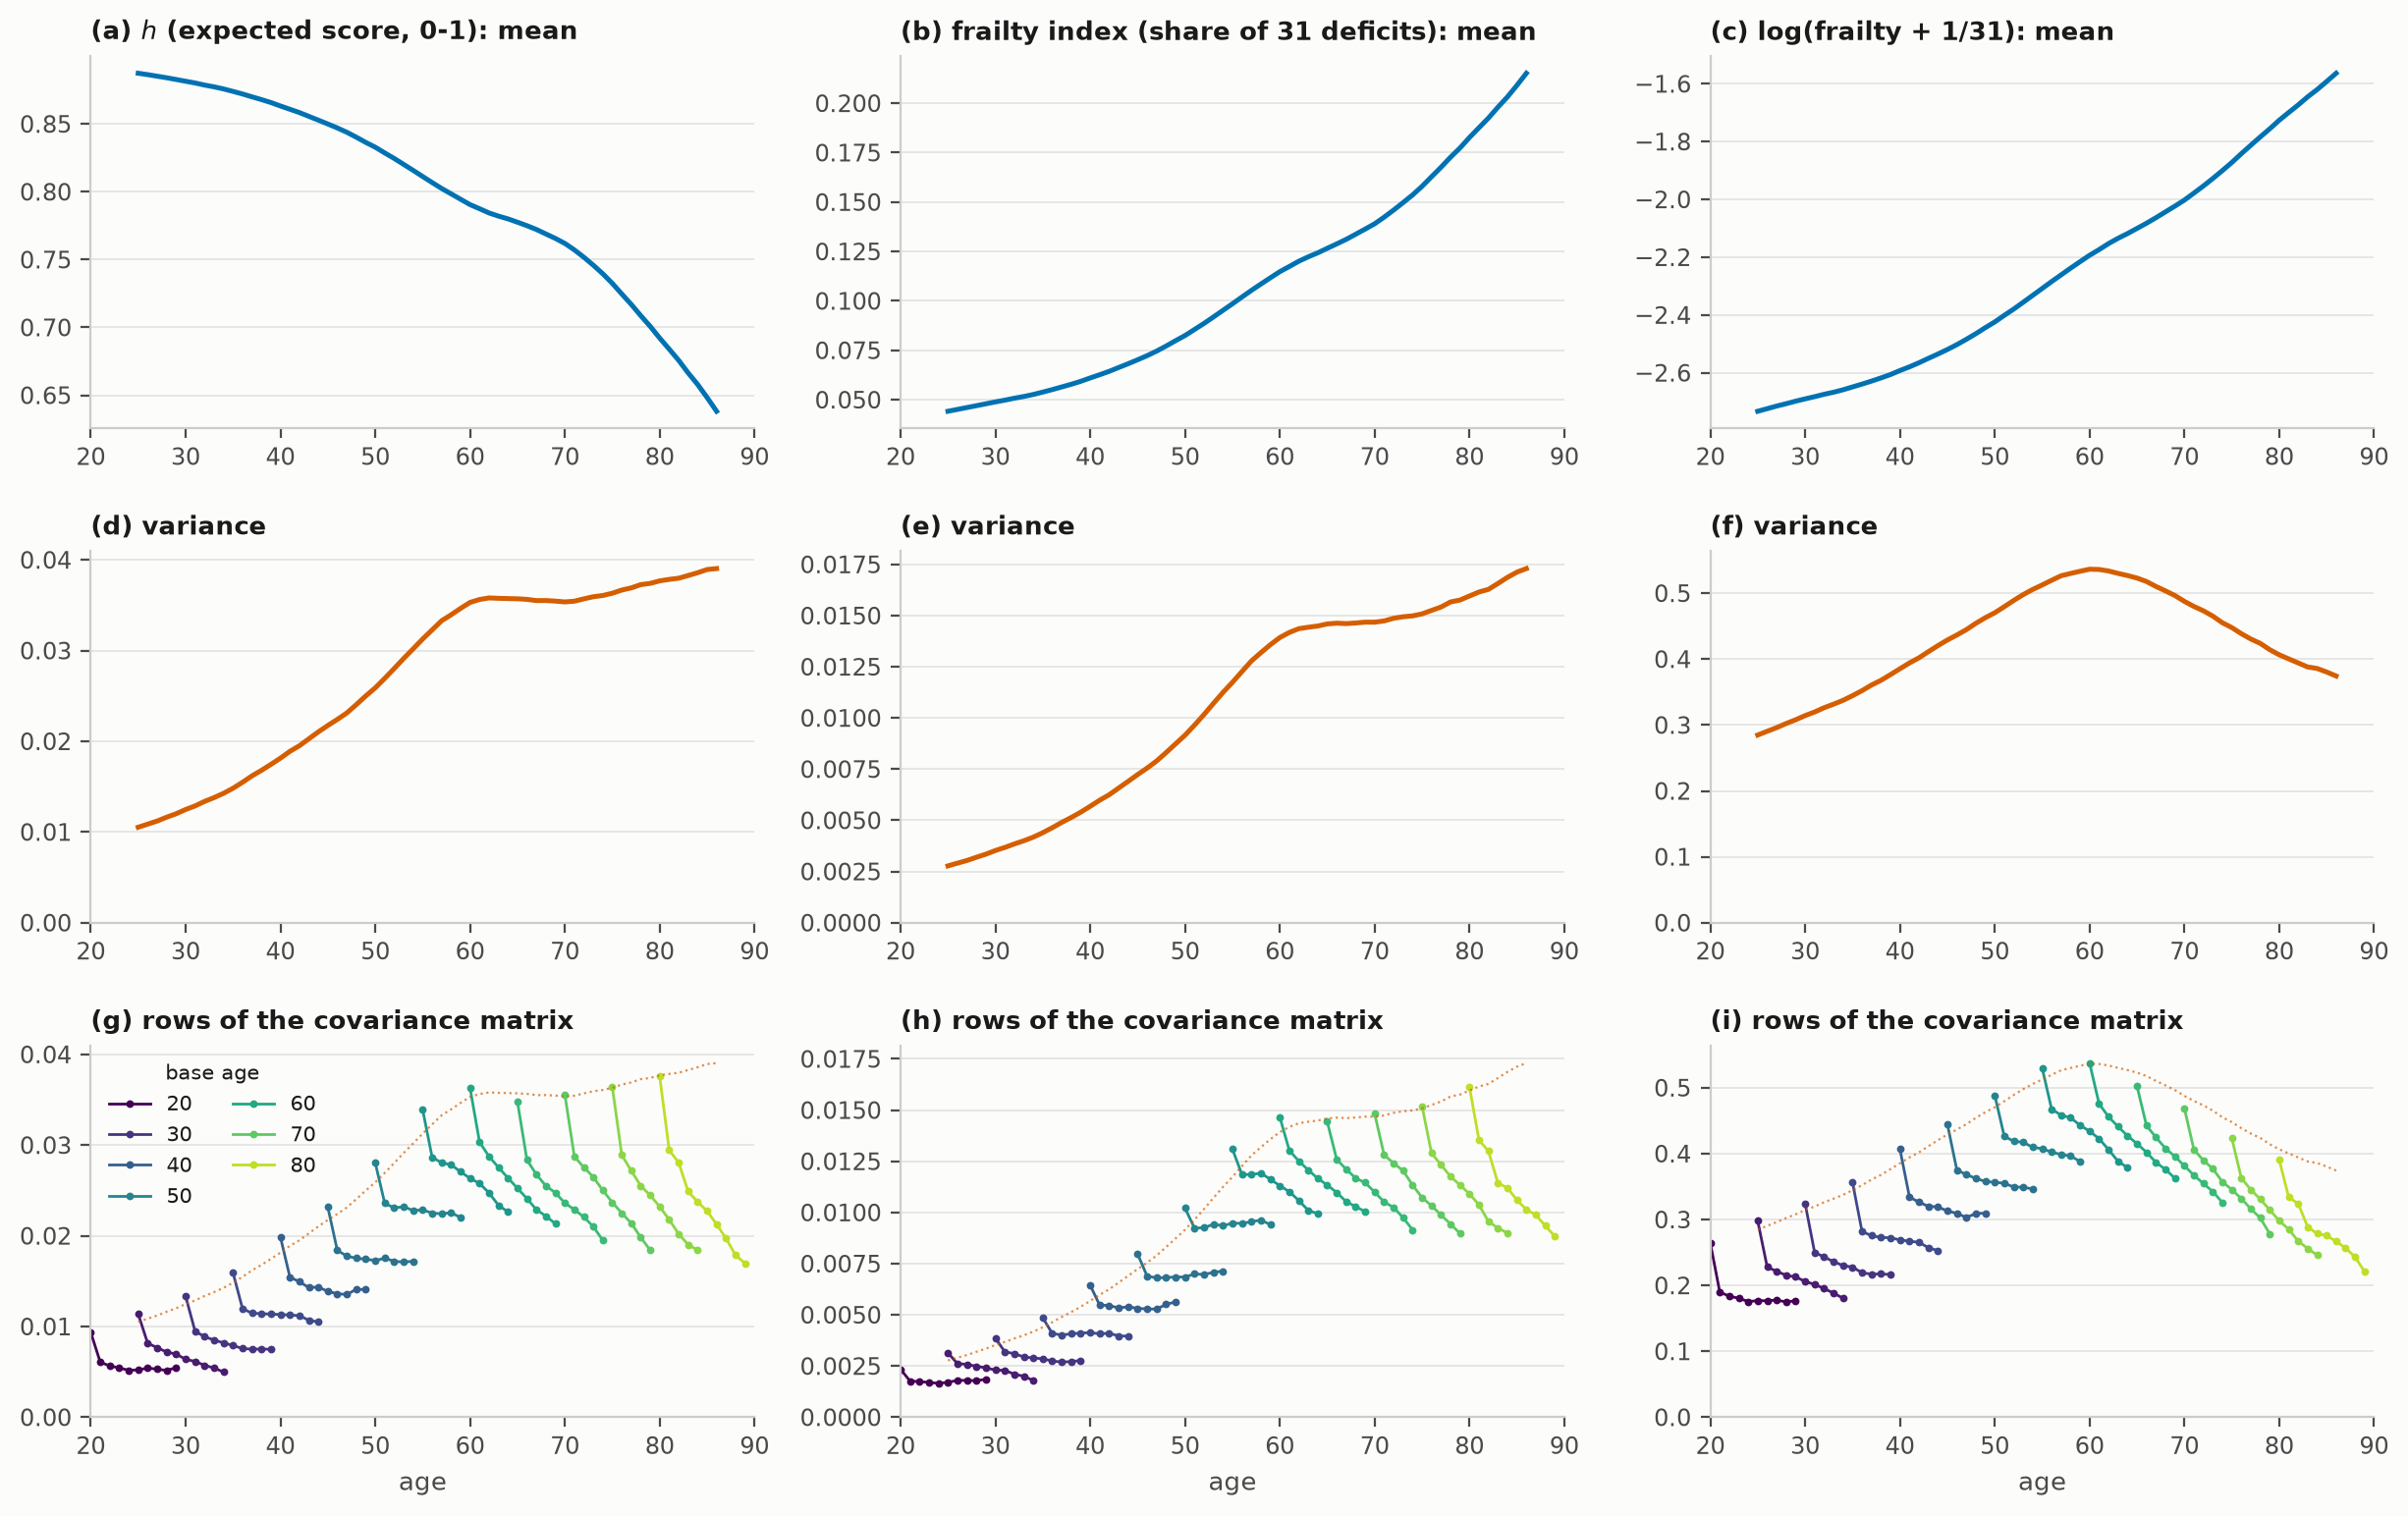
\includegraphics[width=\linewidth]{fig_exhibit1_measures.png}
	\caption{As Figure~\ref{fig:exhibit1}, on $h$, frailty and log frailty.}
	\label{fig:exhibit1_measures}
\end{figure}
\begin{figure}[H]\centering
	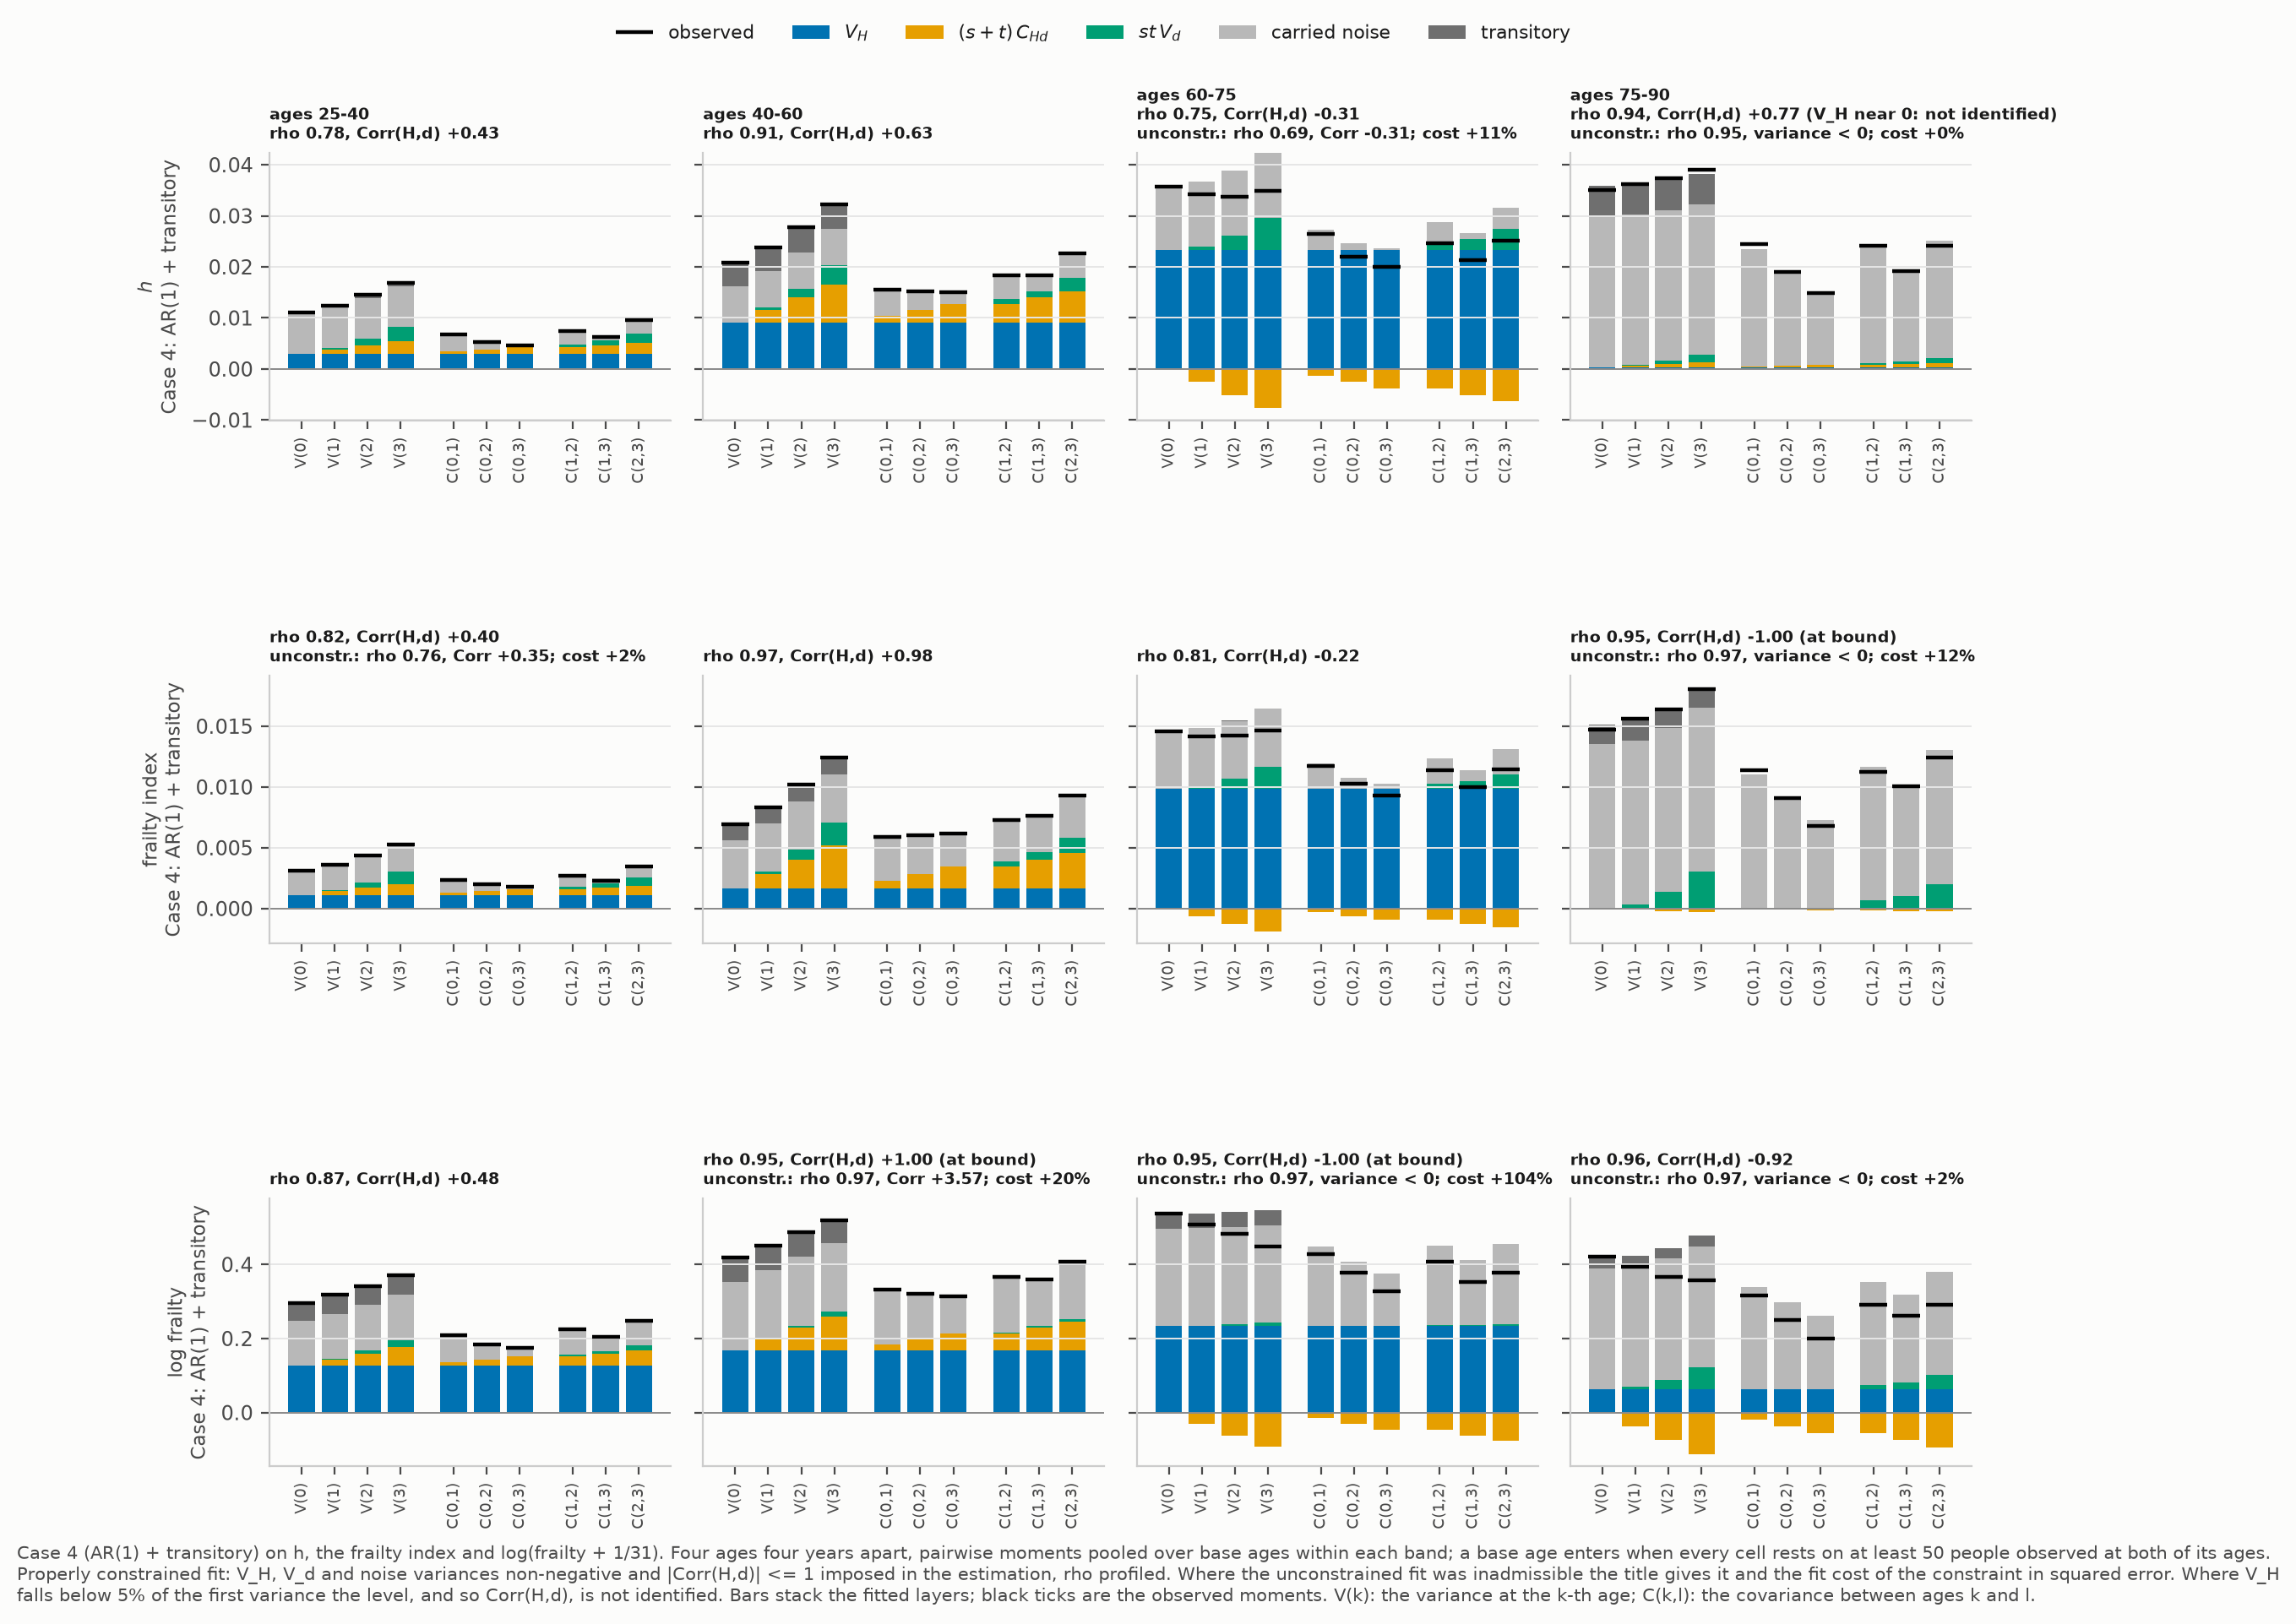
\includegraphics[width=\linewidth]{fig_exhibit2_measures.png}
	\caption{As Figure~\ref{fig:ex2main}, on $h$, frailty and log frailty.}
	\label{fig:ex2measures}
\end{figure}
\begin{figure}[H]\centering
	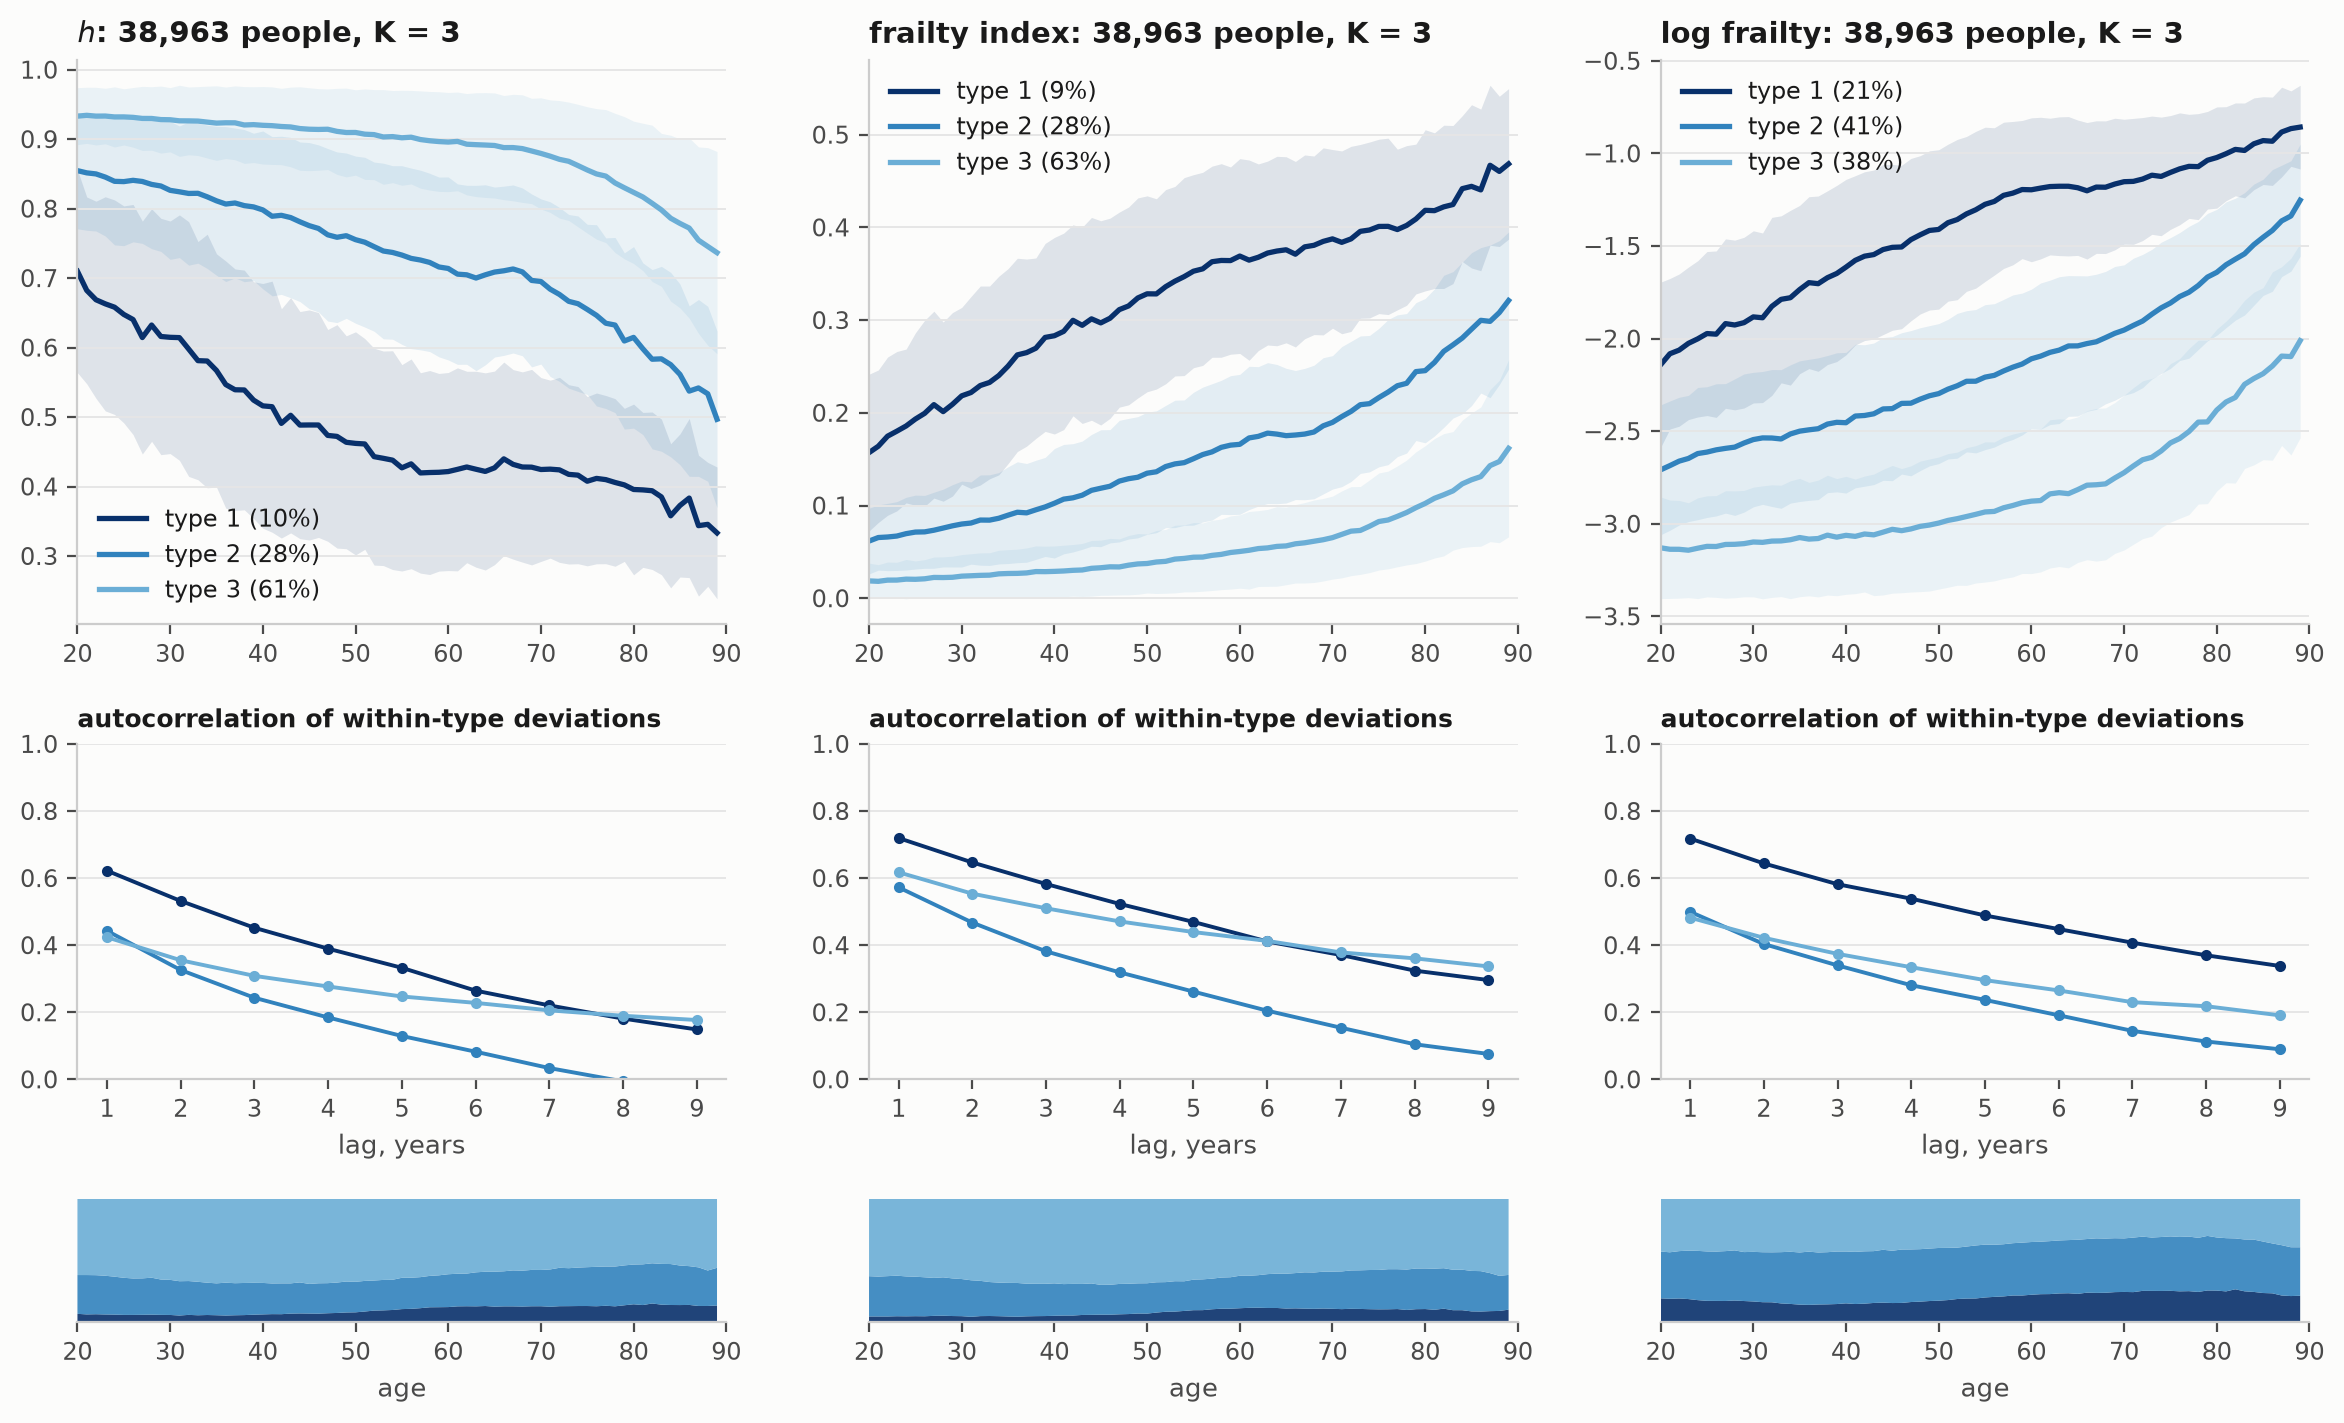
\includegraphics[width=\linewidth]{fig_clusters_measures.png}
	\caption{As Figure~\ref{fig:clusters}, on $h$, frailty and log frailty.}
	\label{fig:clusters_measures}
\end{figure}
\begin{figure}[H]\centering
	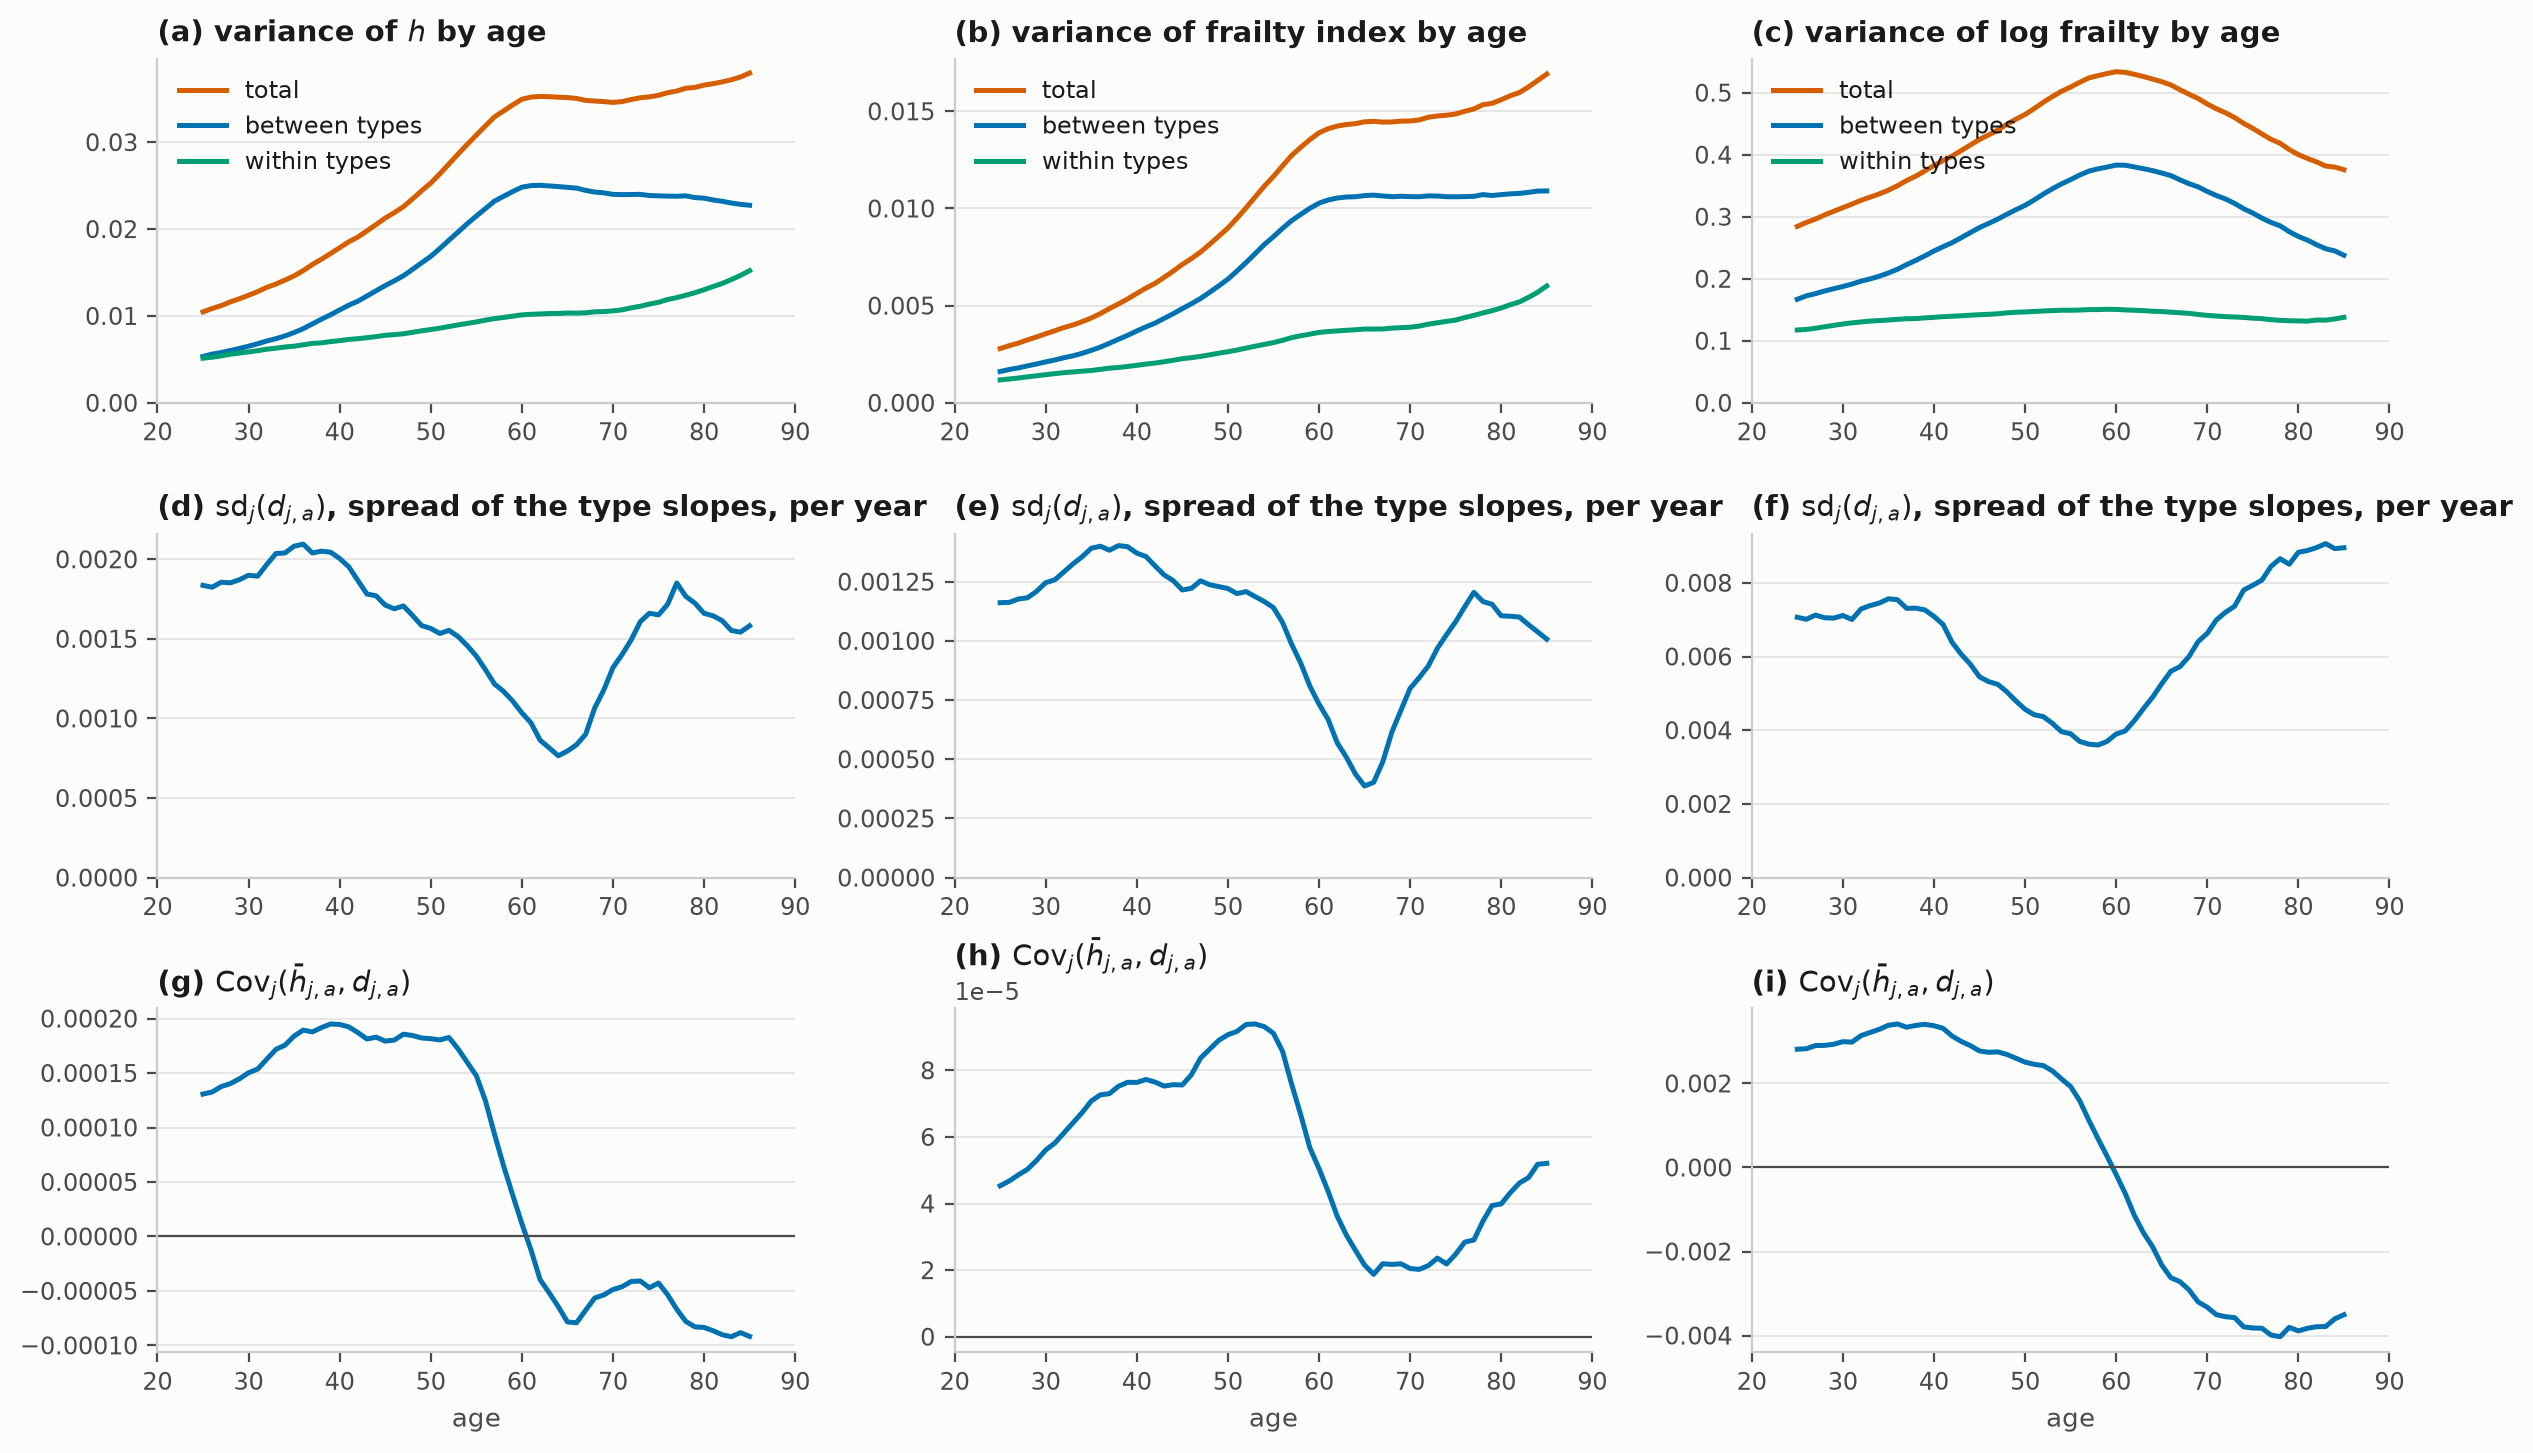
\includegraphics[width=\linewidth]{fig_cluster_decomposition_measures.png}
	\caption{As Figure~\ref{fig:decomp}, on $h$, frailty and log frailty.}
	\label{fig:decomp_measures}
\end{figure}
\begin{figure}[H]\centering
	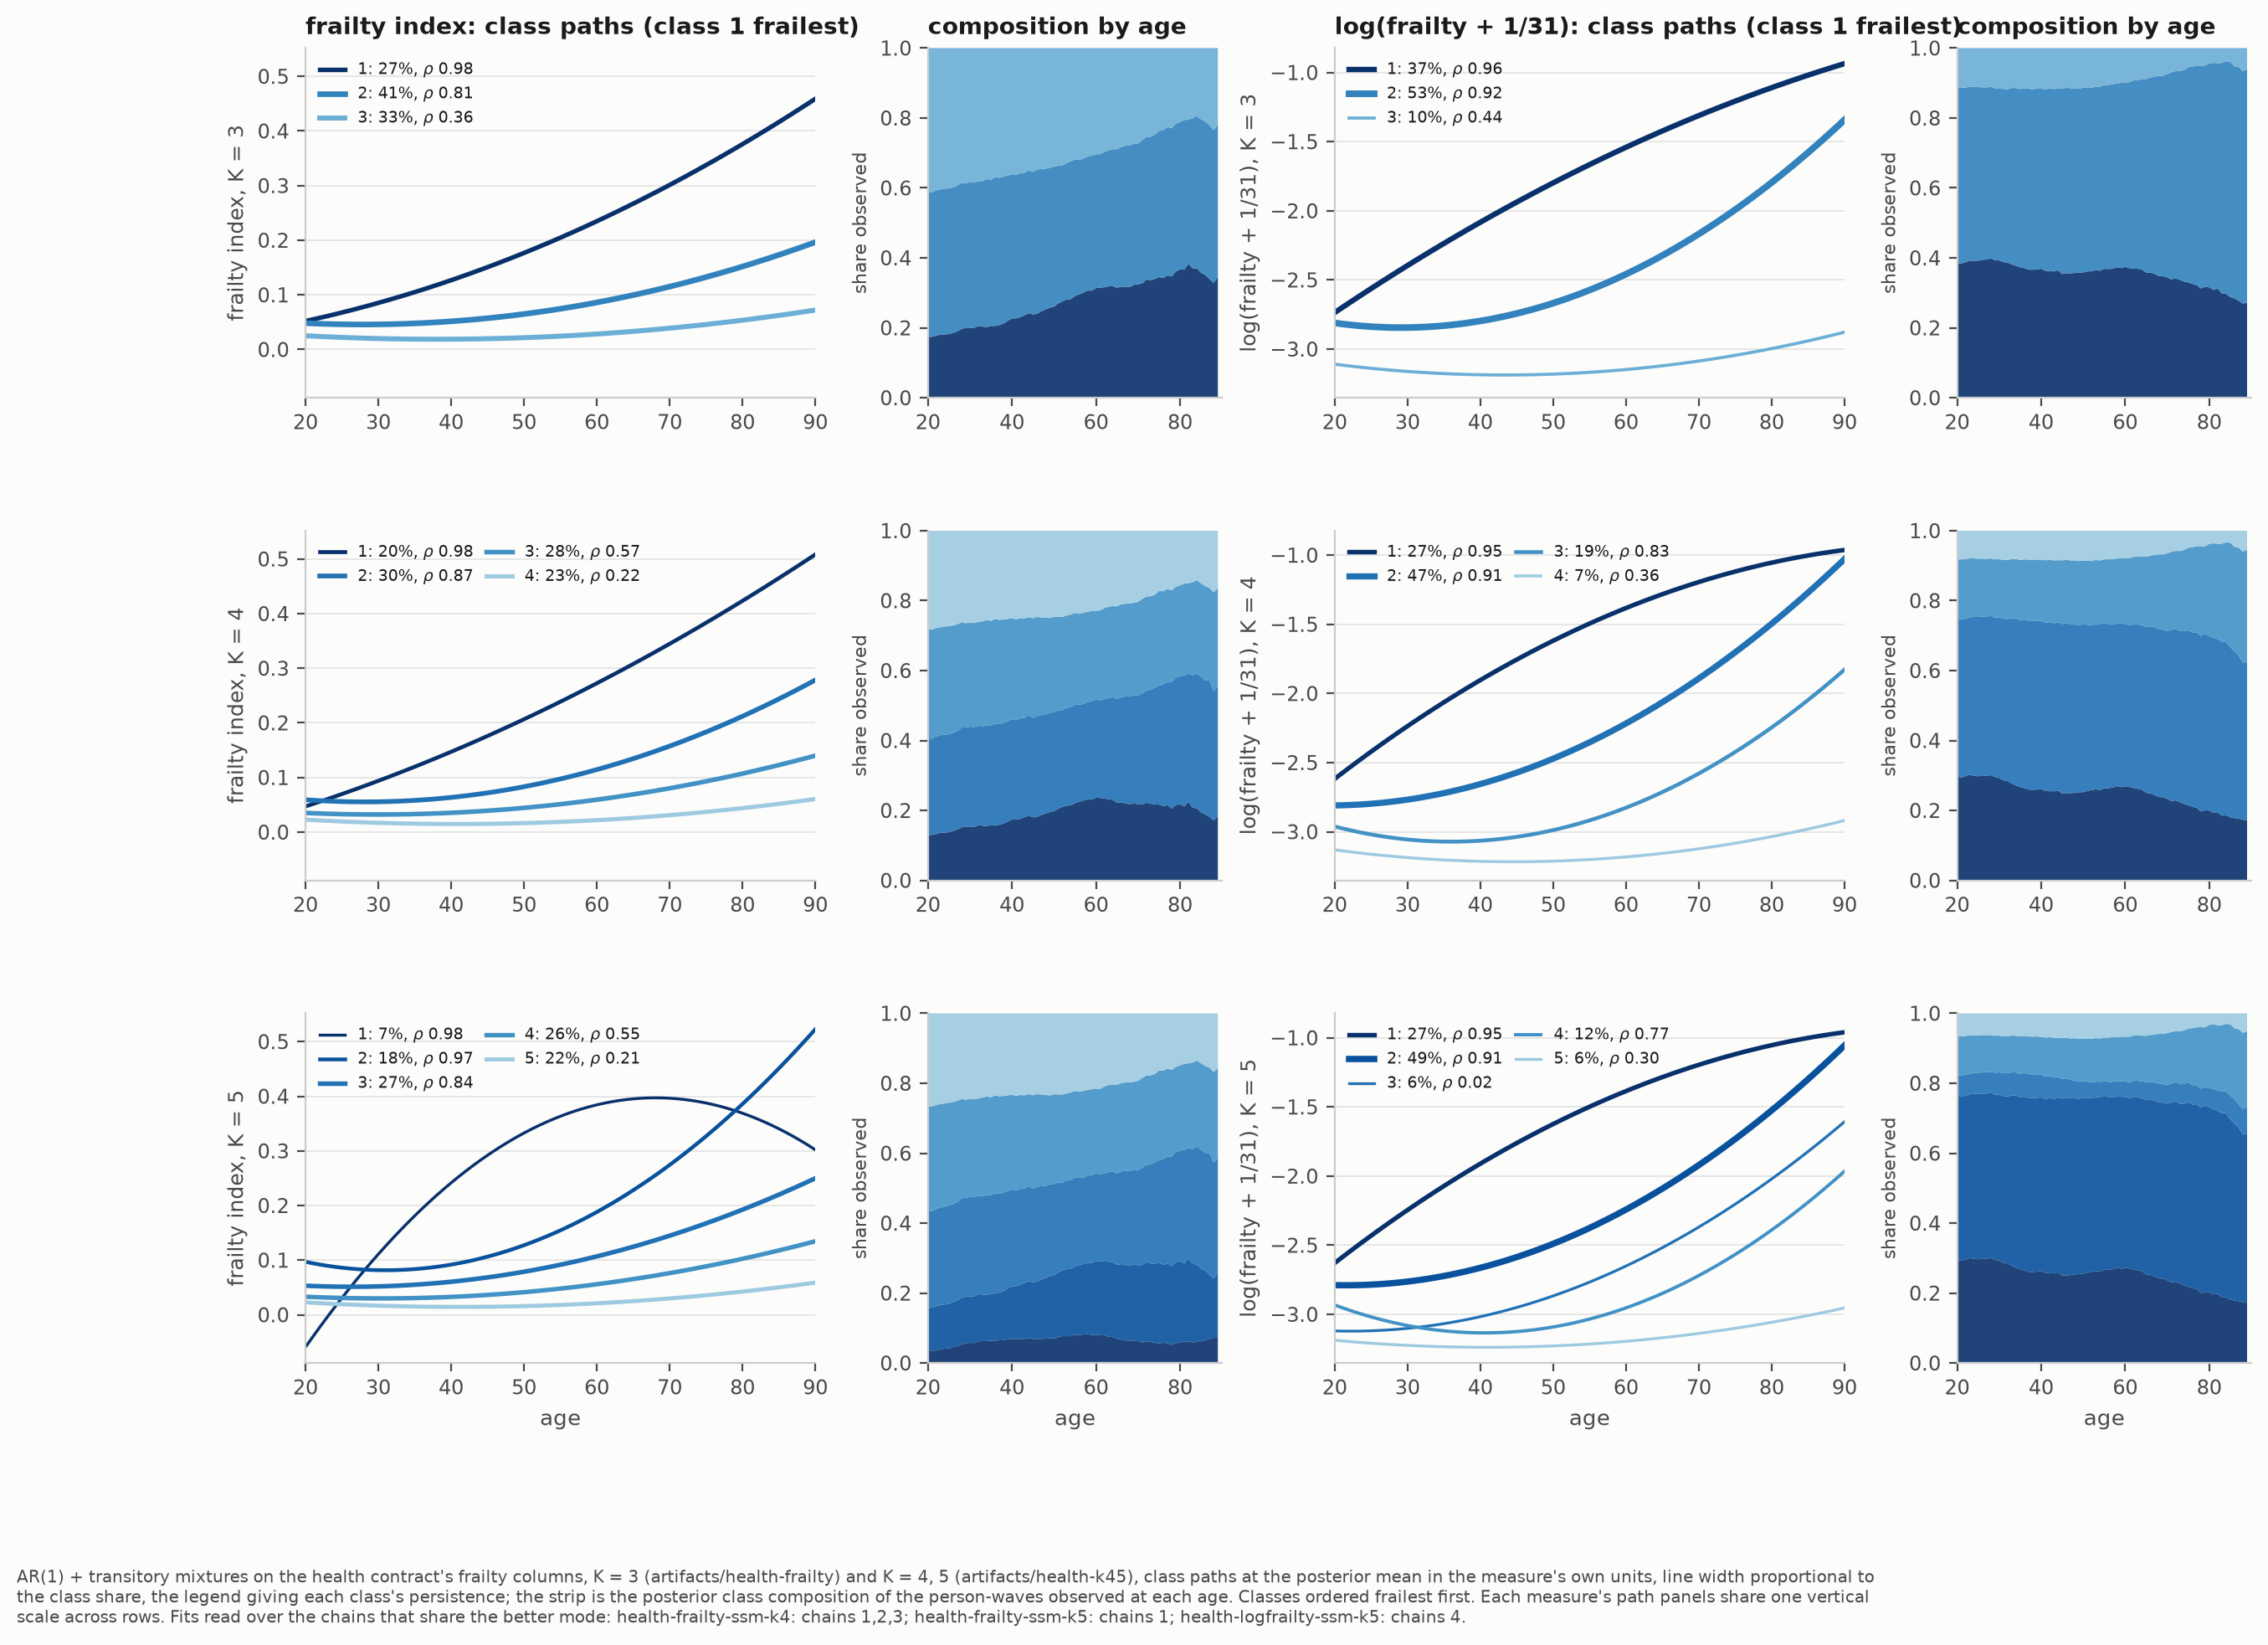
\includegraphics[width=\linewidth]{fig_frailty_by_K.png}
	\caption{Frailty and log frailty under the persistent--transitory specification at $K=3,4,5$.}
	\label{fig:frailty_by_K}
\end{figure}
\begin{figure}[H]\centering
	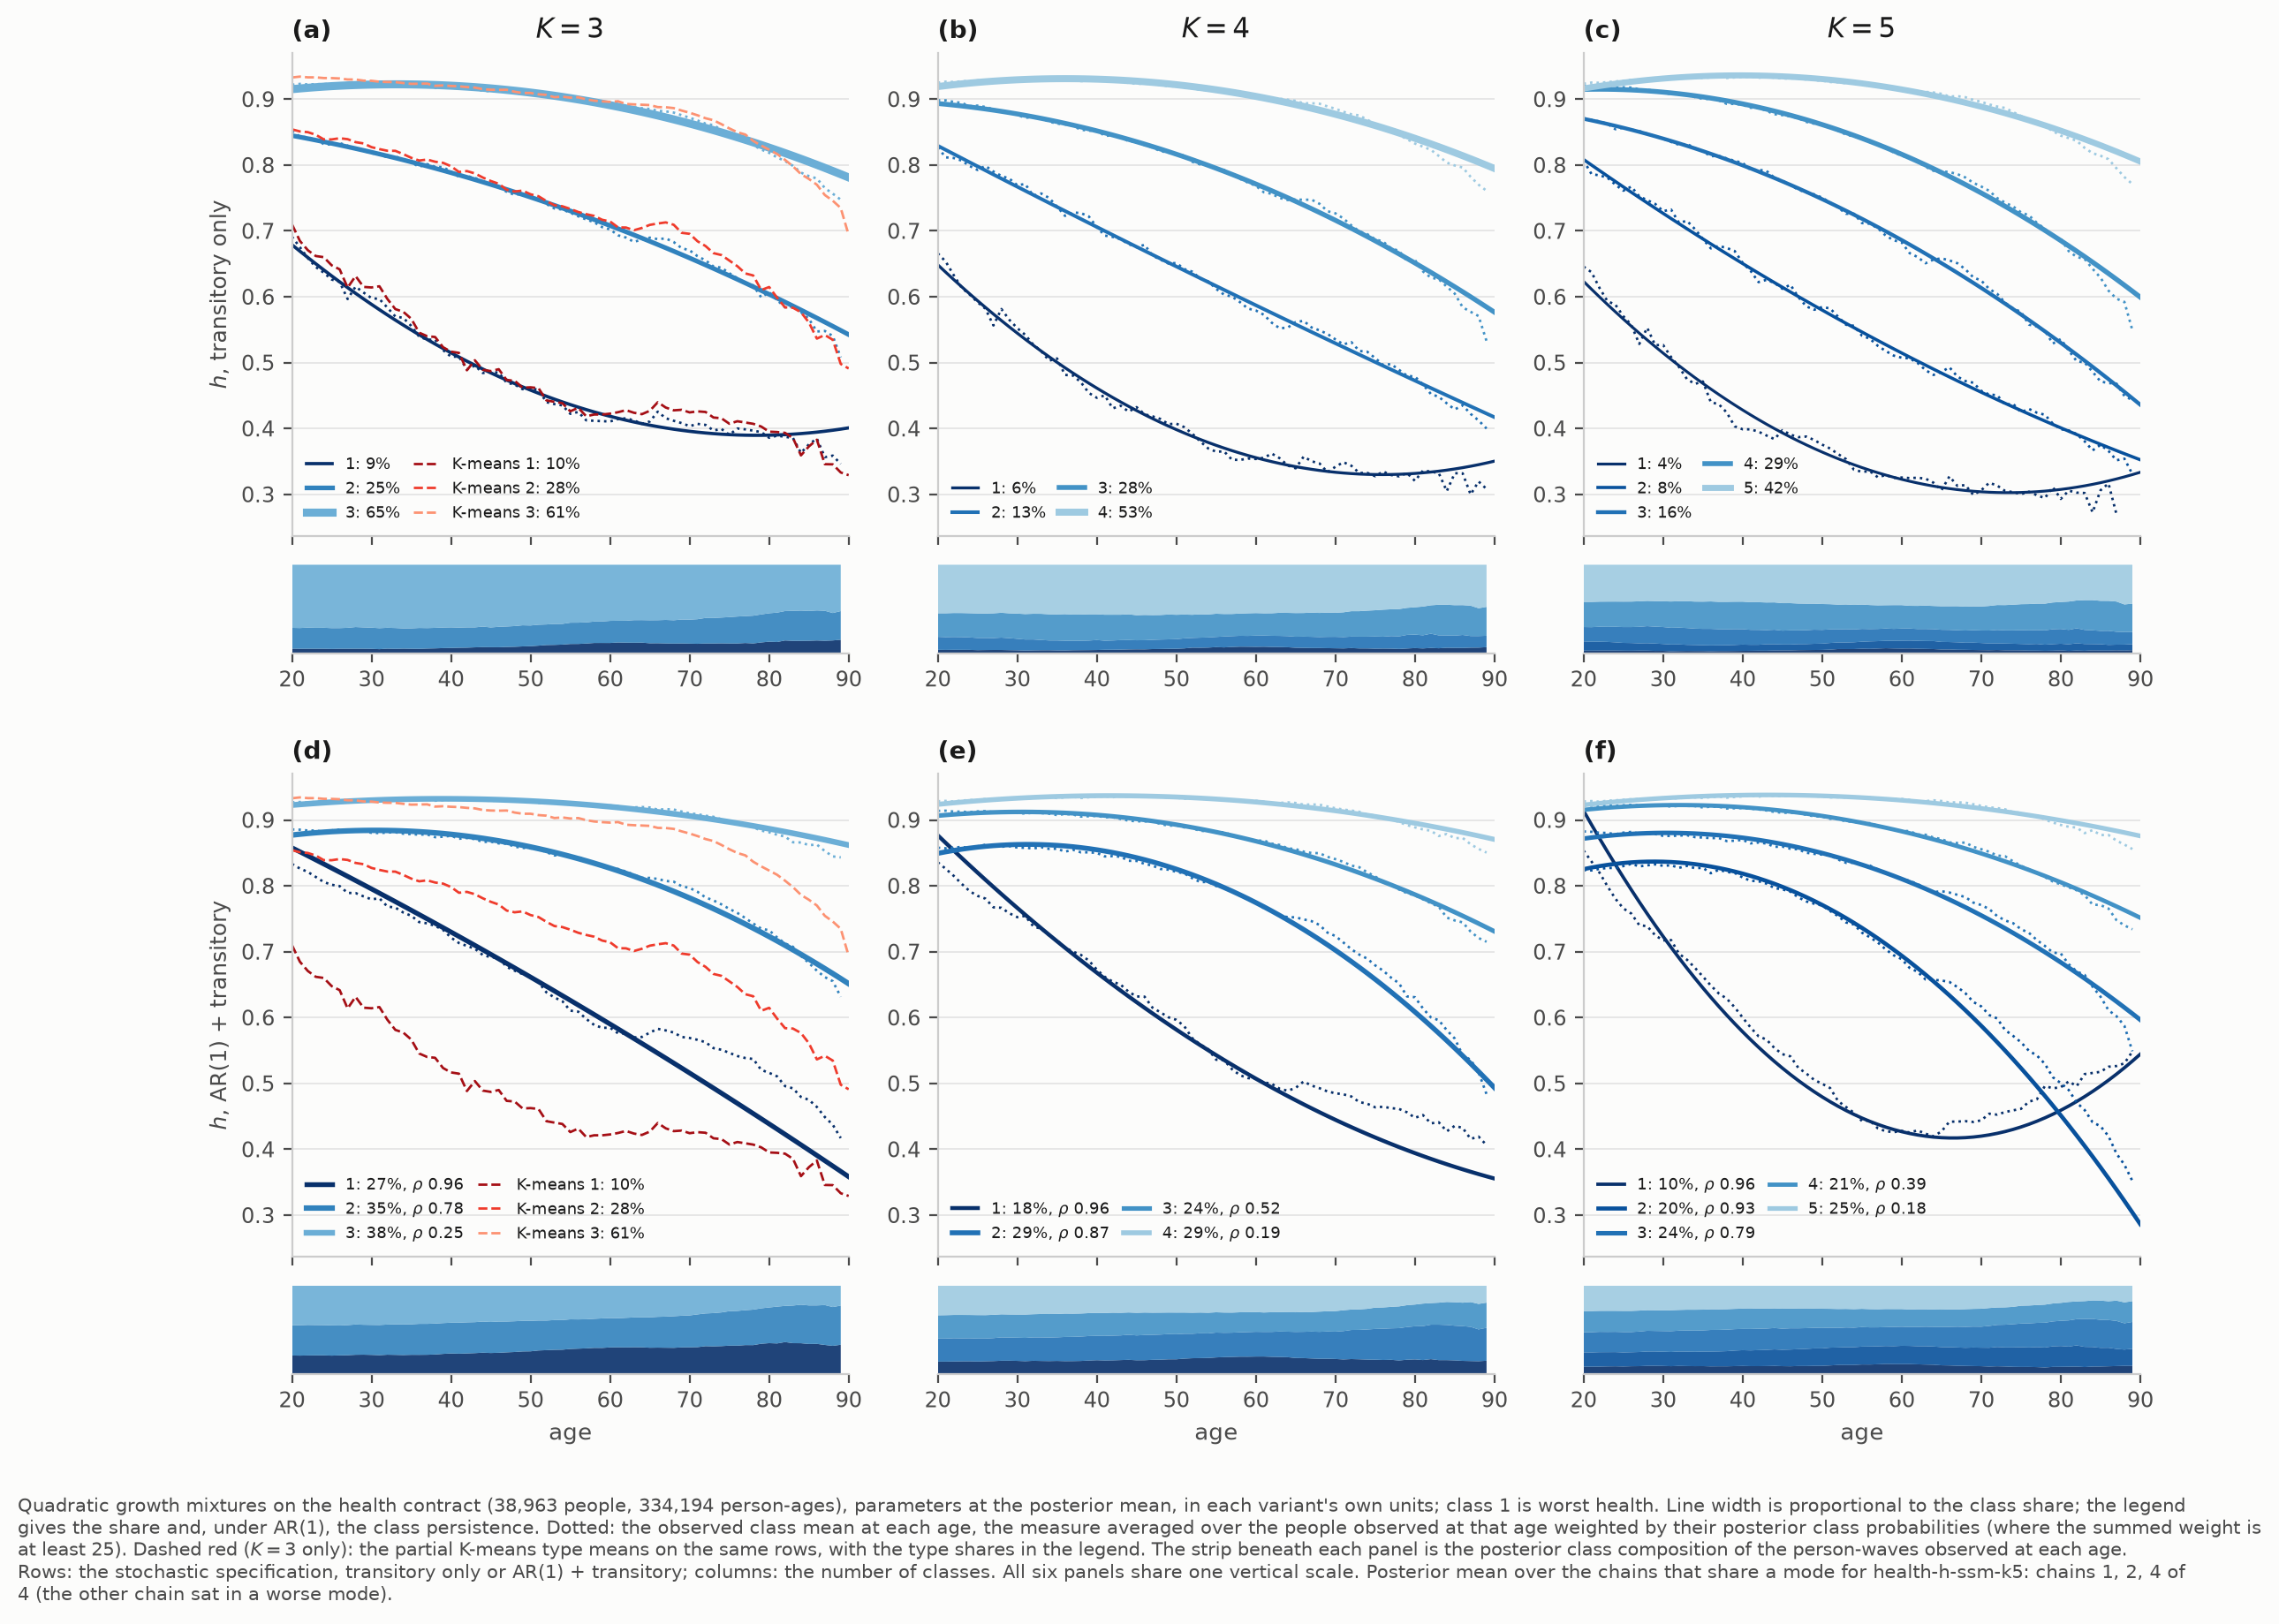
\includegraphics[width=\linewidth]{fig_class_trajectories_by_K_h.png}
	\caption{As Figure~\ref{fig:trajK}, on $h$.}
	\label{fig:trajK_h}
\end{figure}
\begin{figure}[H]\centering
	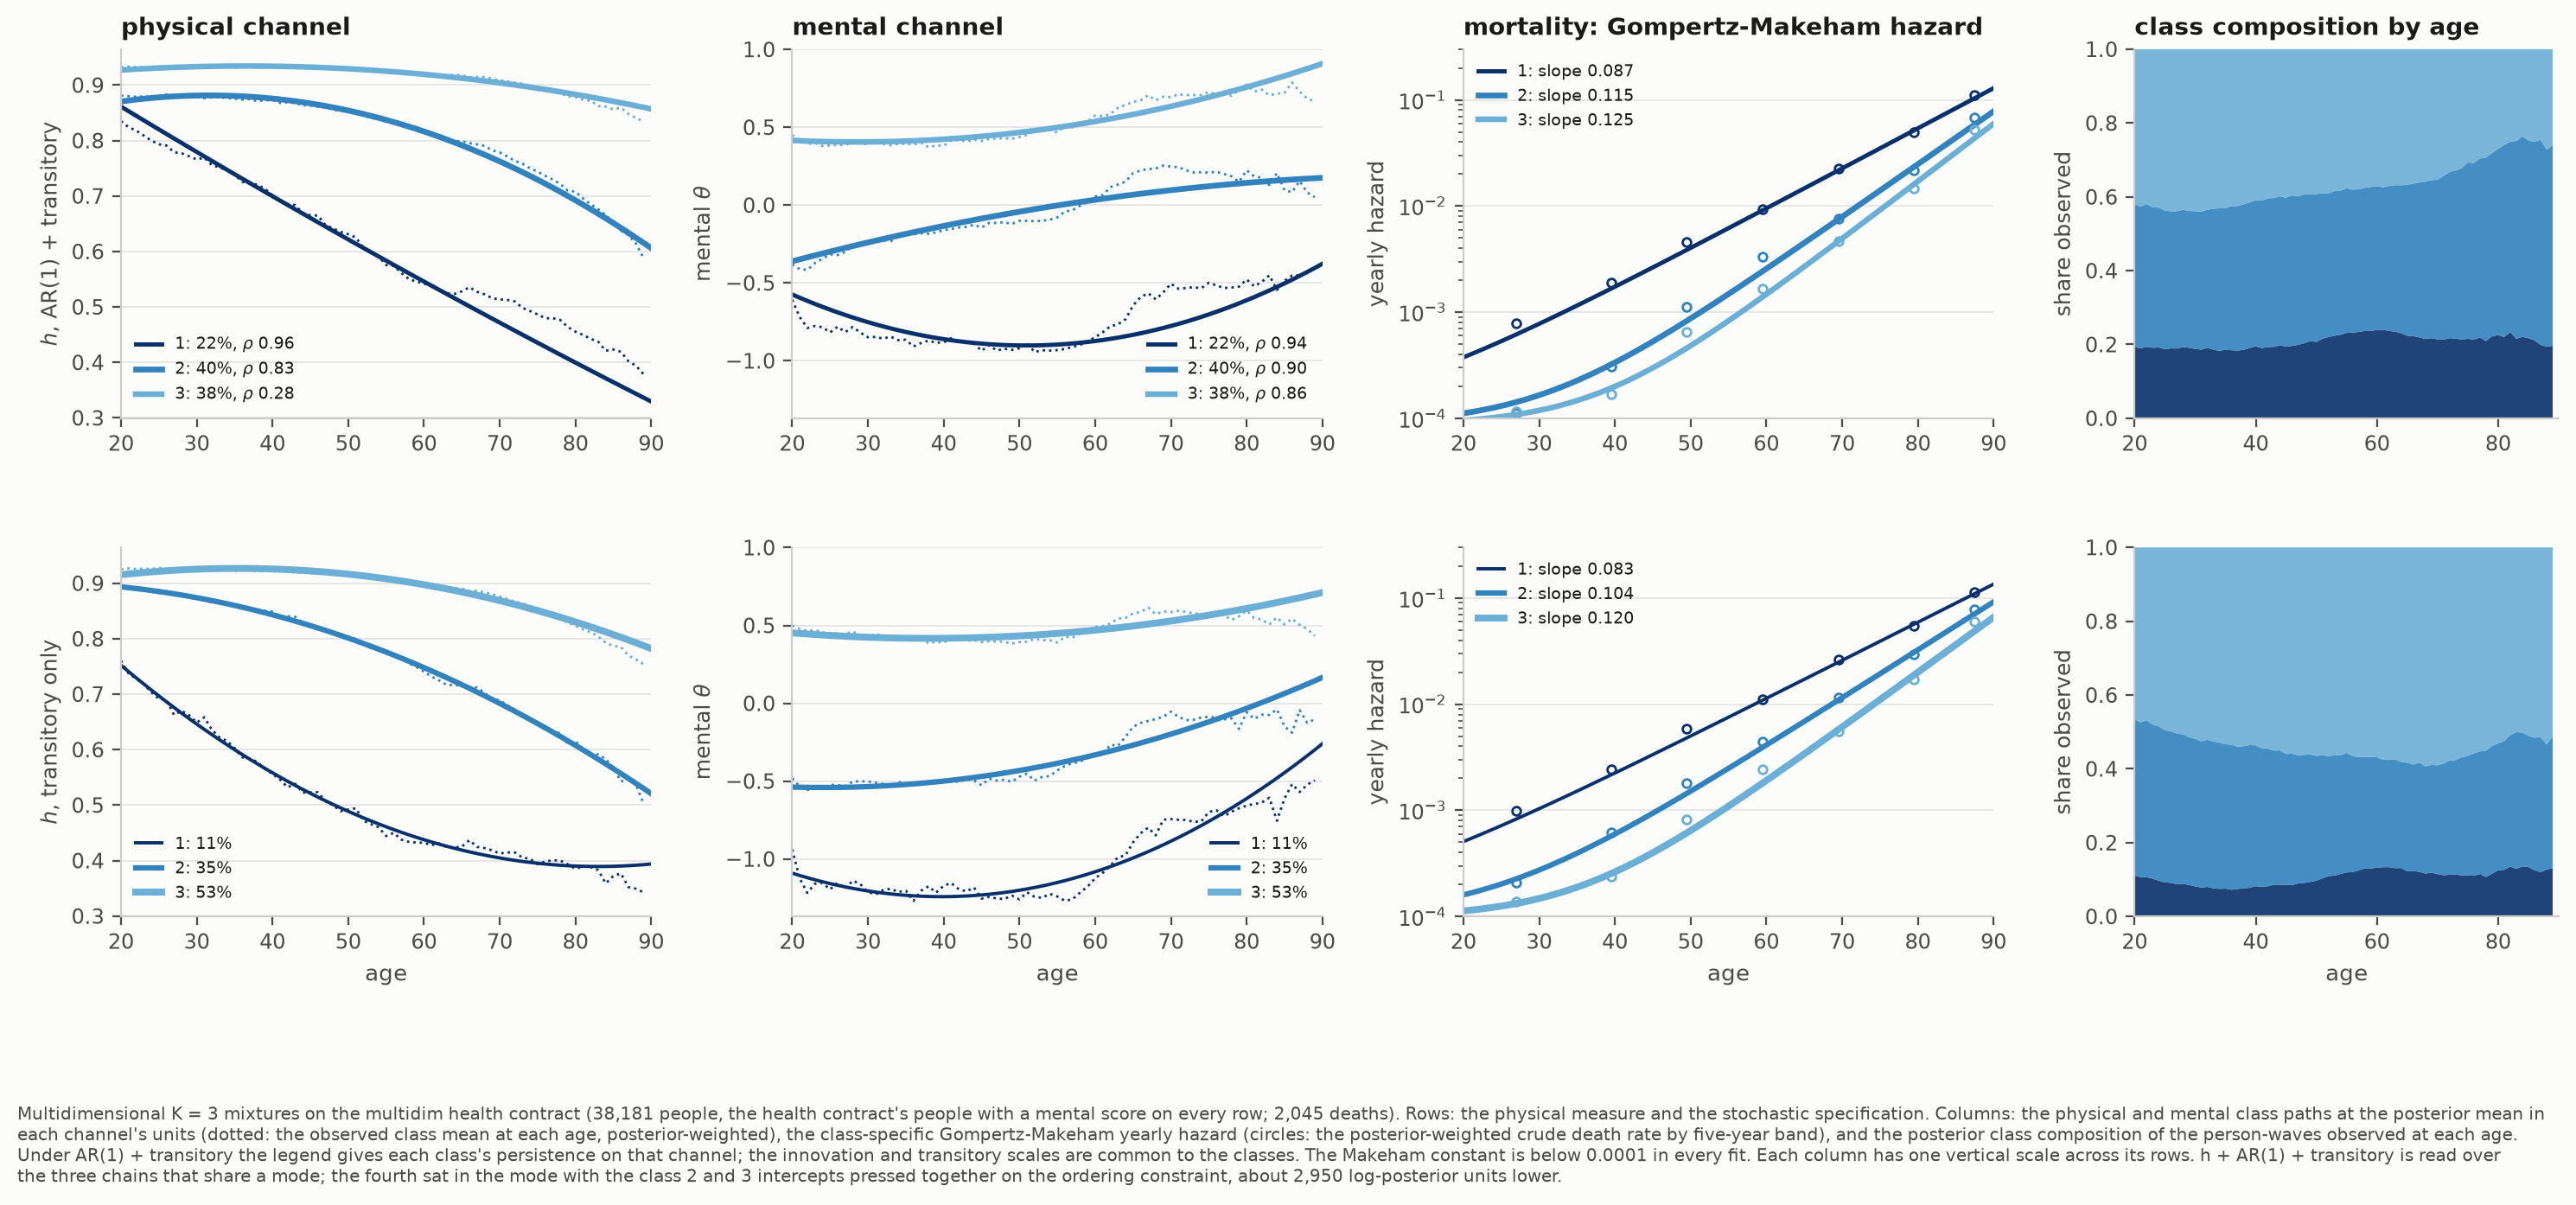
\includegraphics[width=\linewidth]{fig_multidim_trajectories_h.png}
	\caption{As Figure~\ref{fig:multidim}, on $h$.}
	\label{fig:multidim_h}
\end{figure}
\begin{figure}[H]\centering
	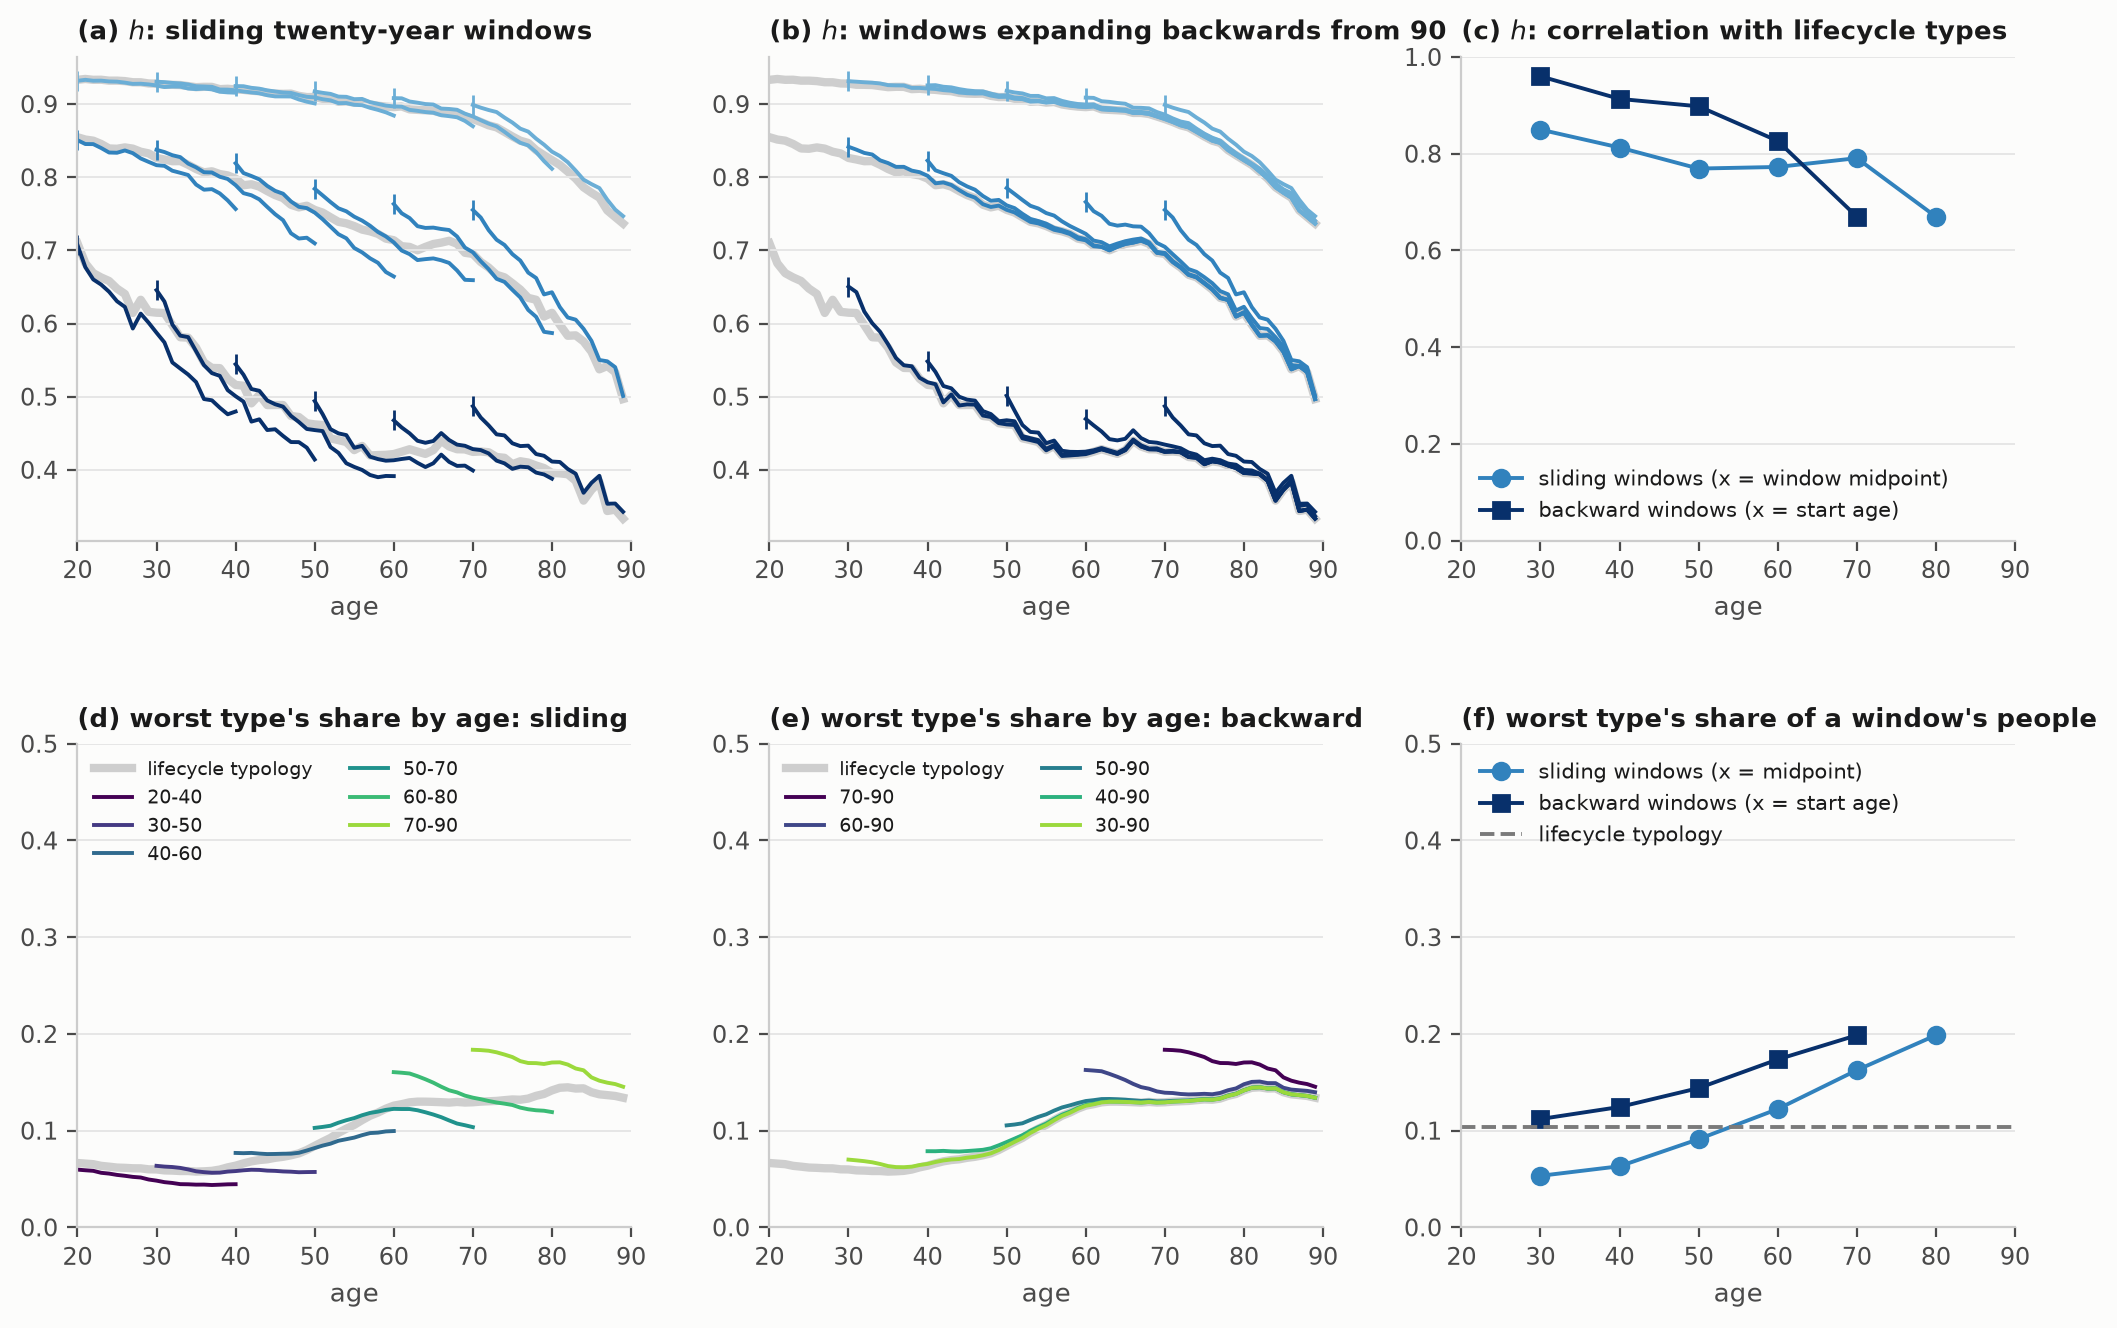
\includegraphics[width=\linewidth]{fig_windows_h.png}
	\caption{As Figure~\ref{fig:windows_kmeans}, on $h$.}
	\label{fig:windows_h}
\end{figure}
\begin{figure}[H]\centering
	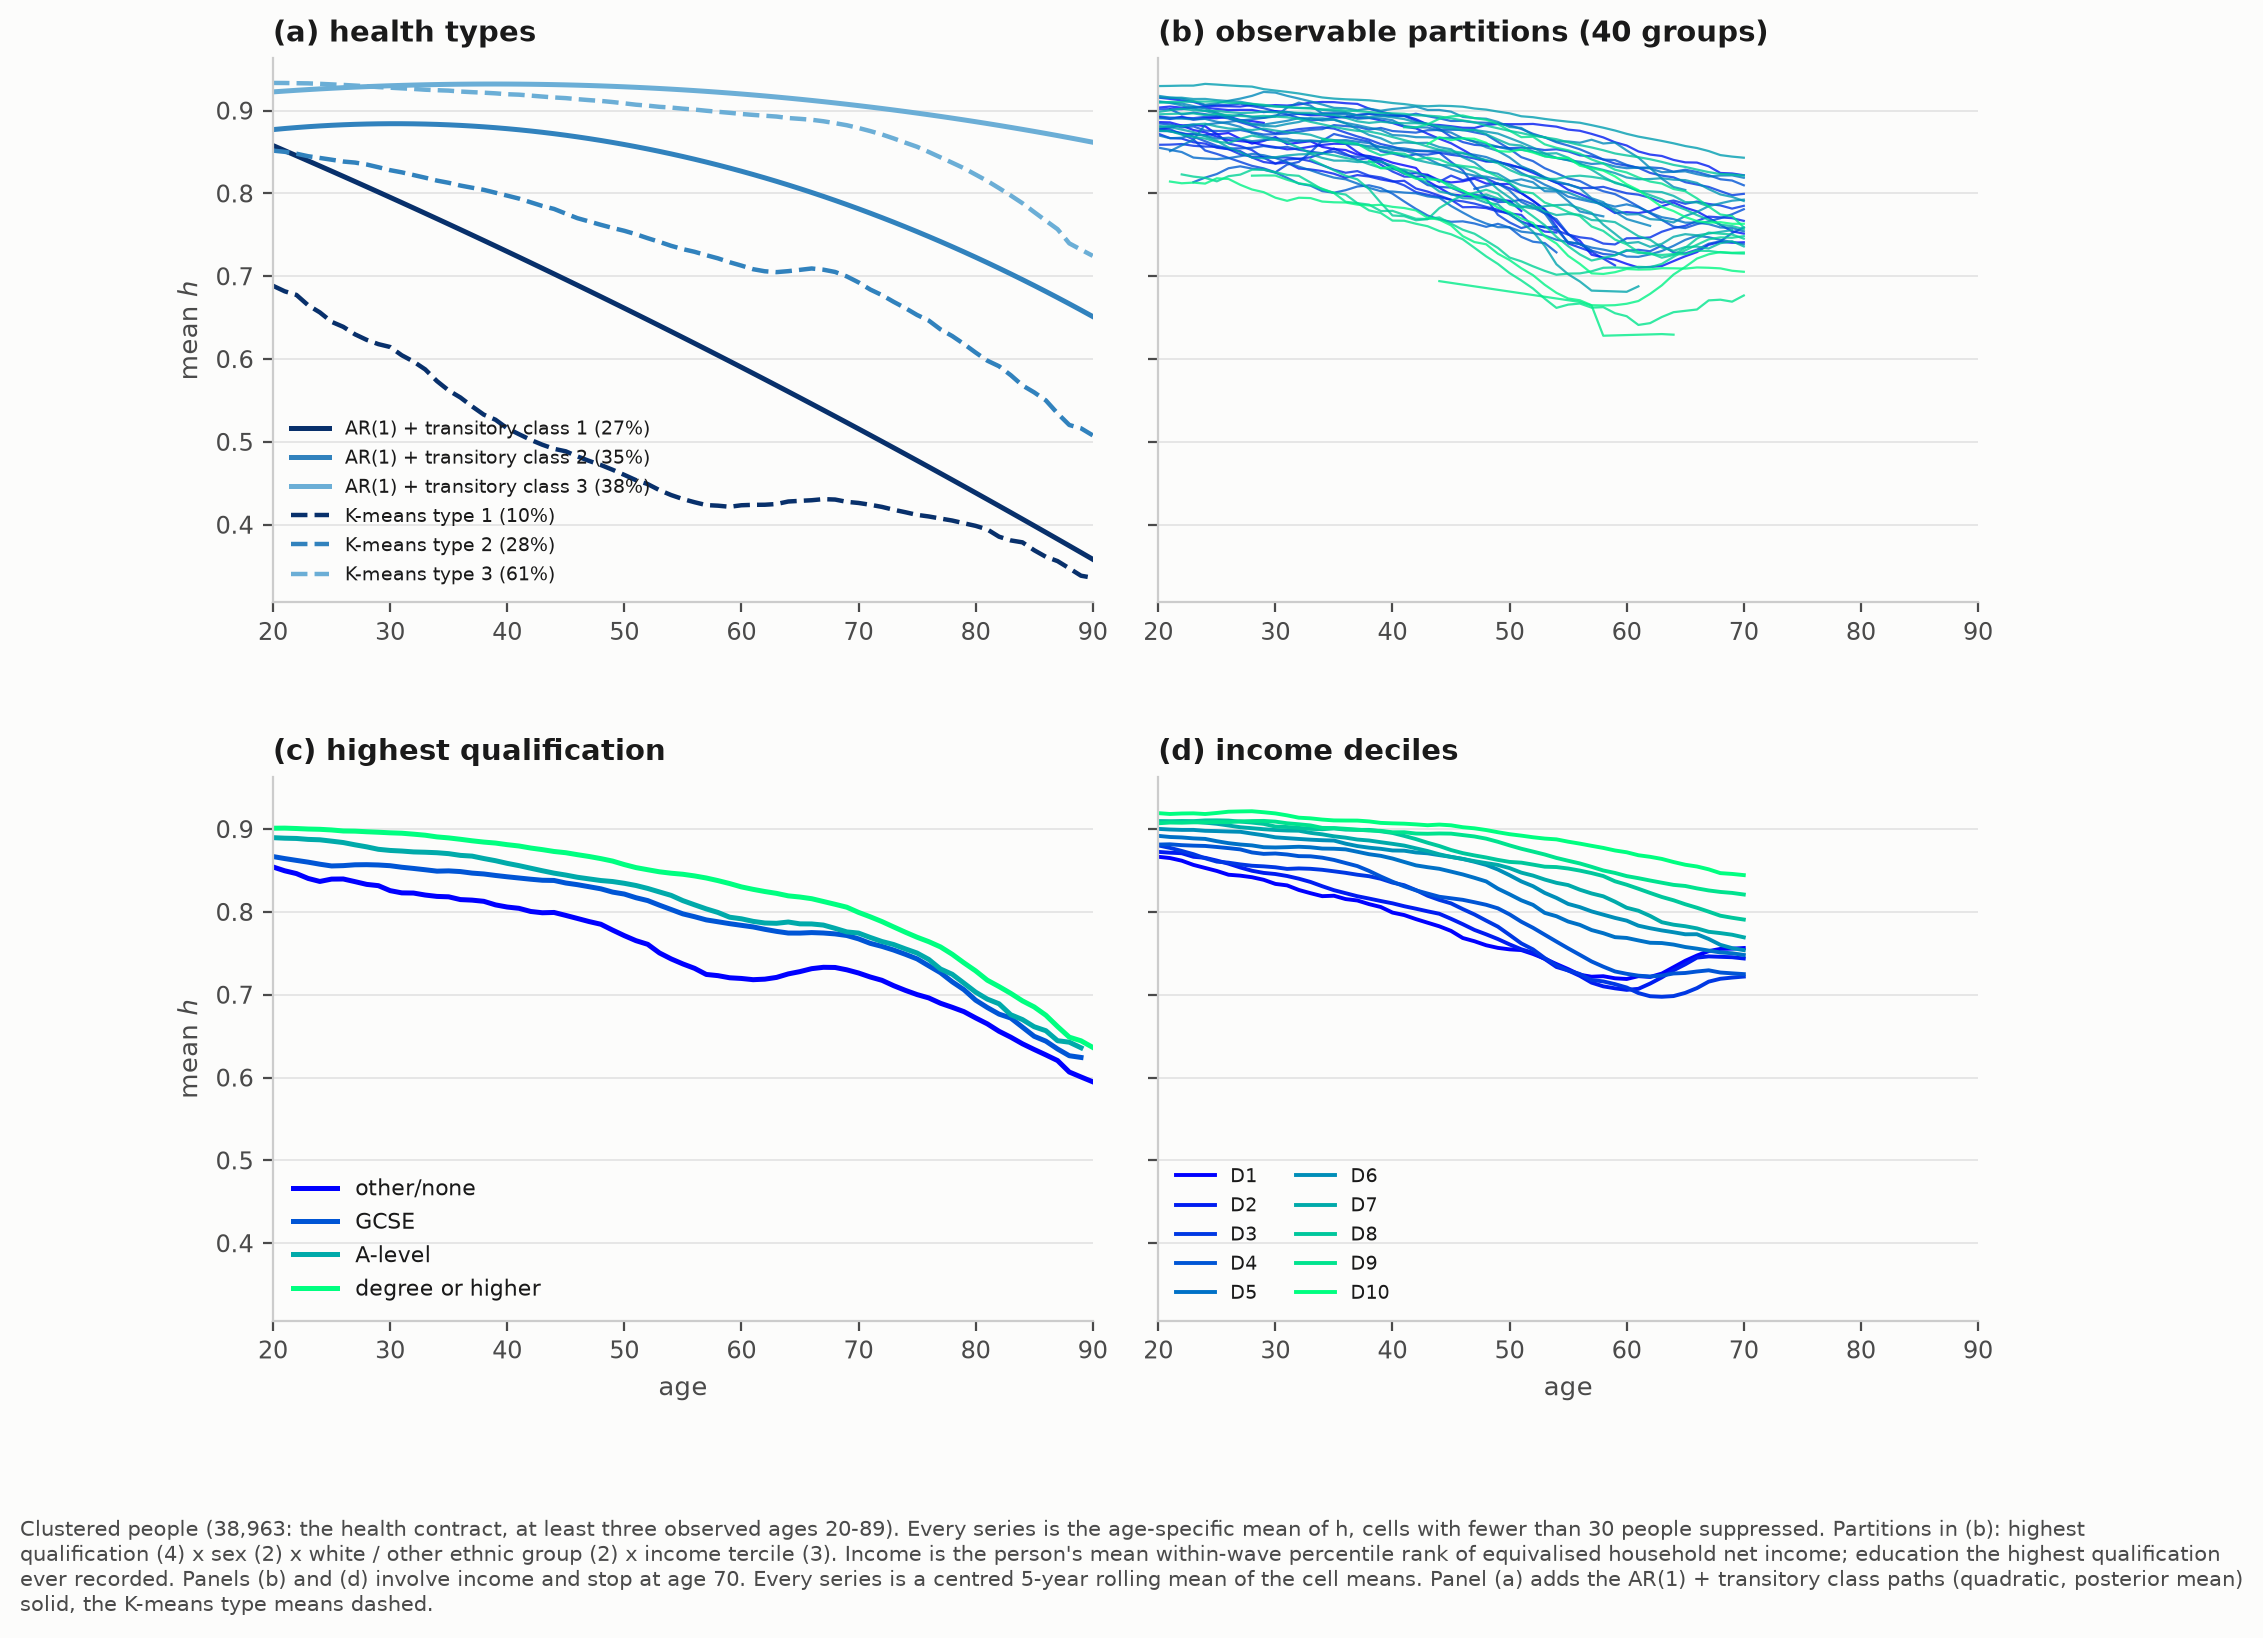
\includegraphics[width=\linewidth]{fig_observables_h.png}
	\caption{As Figure~\ref{fig:obs}, on $h$.}
	\label{fig:obs_h}
\end{figure}
\begin{figure}[H]\centering
	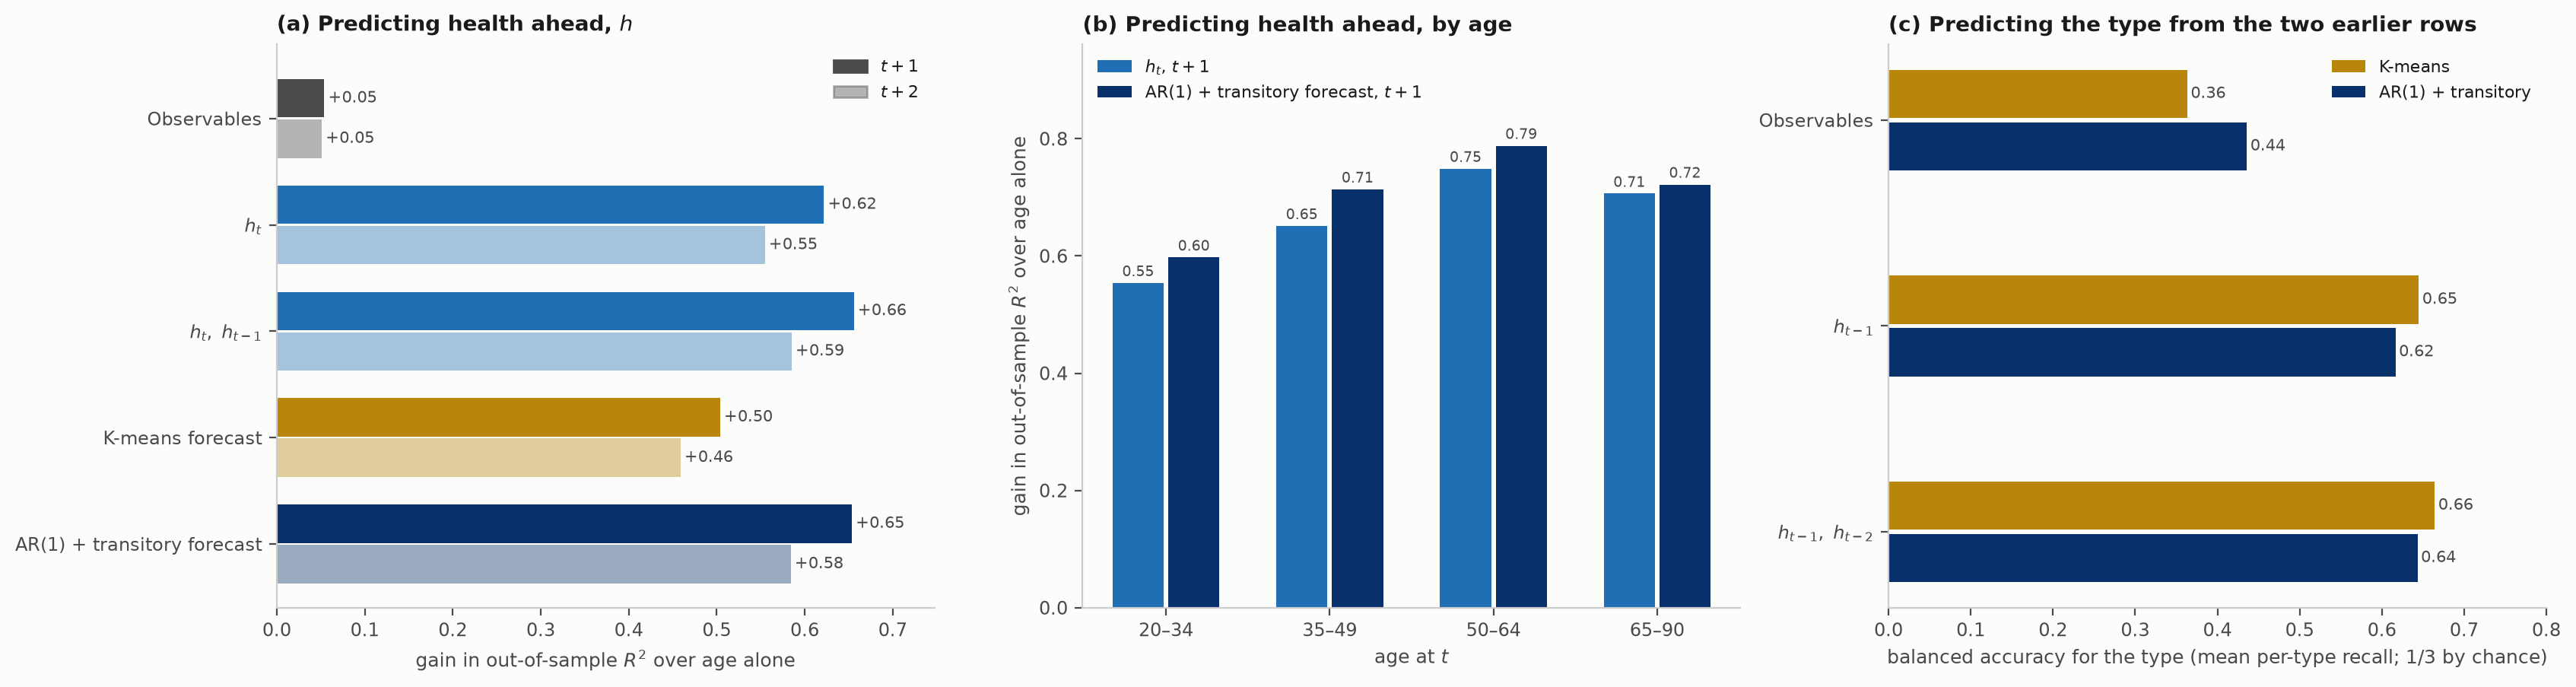
\includegraphics[width=\linewidth]{fig_prediction_summary_h.png}
	\caption{As Figure~\ref{fig:predsummary}, on $h$.}
	\label{fig:predsummary_h}
\end{figure}
\begin{figure}[H]\centering
	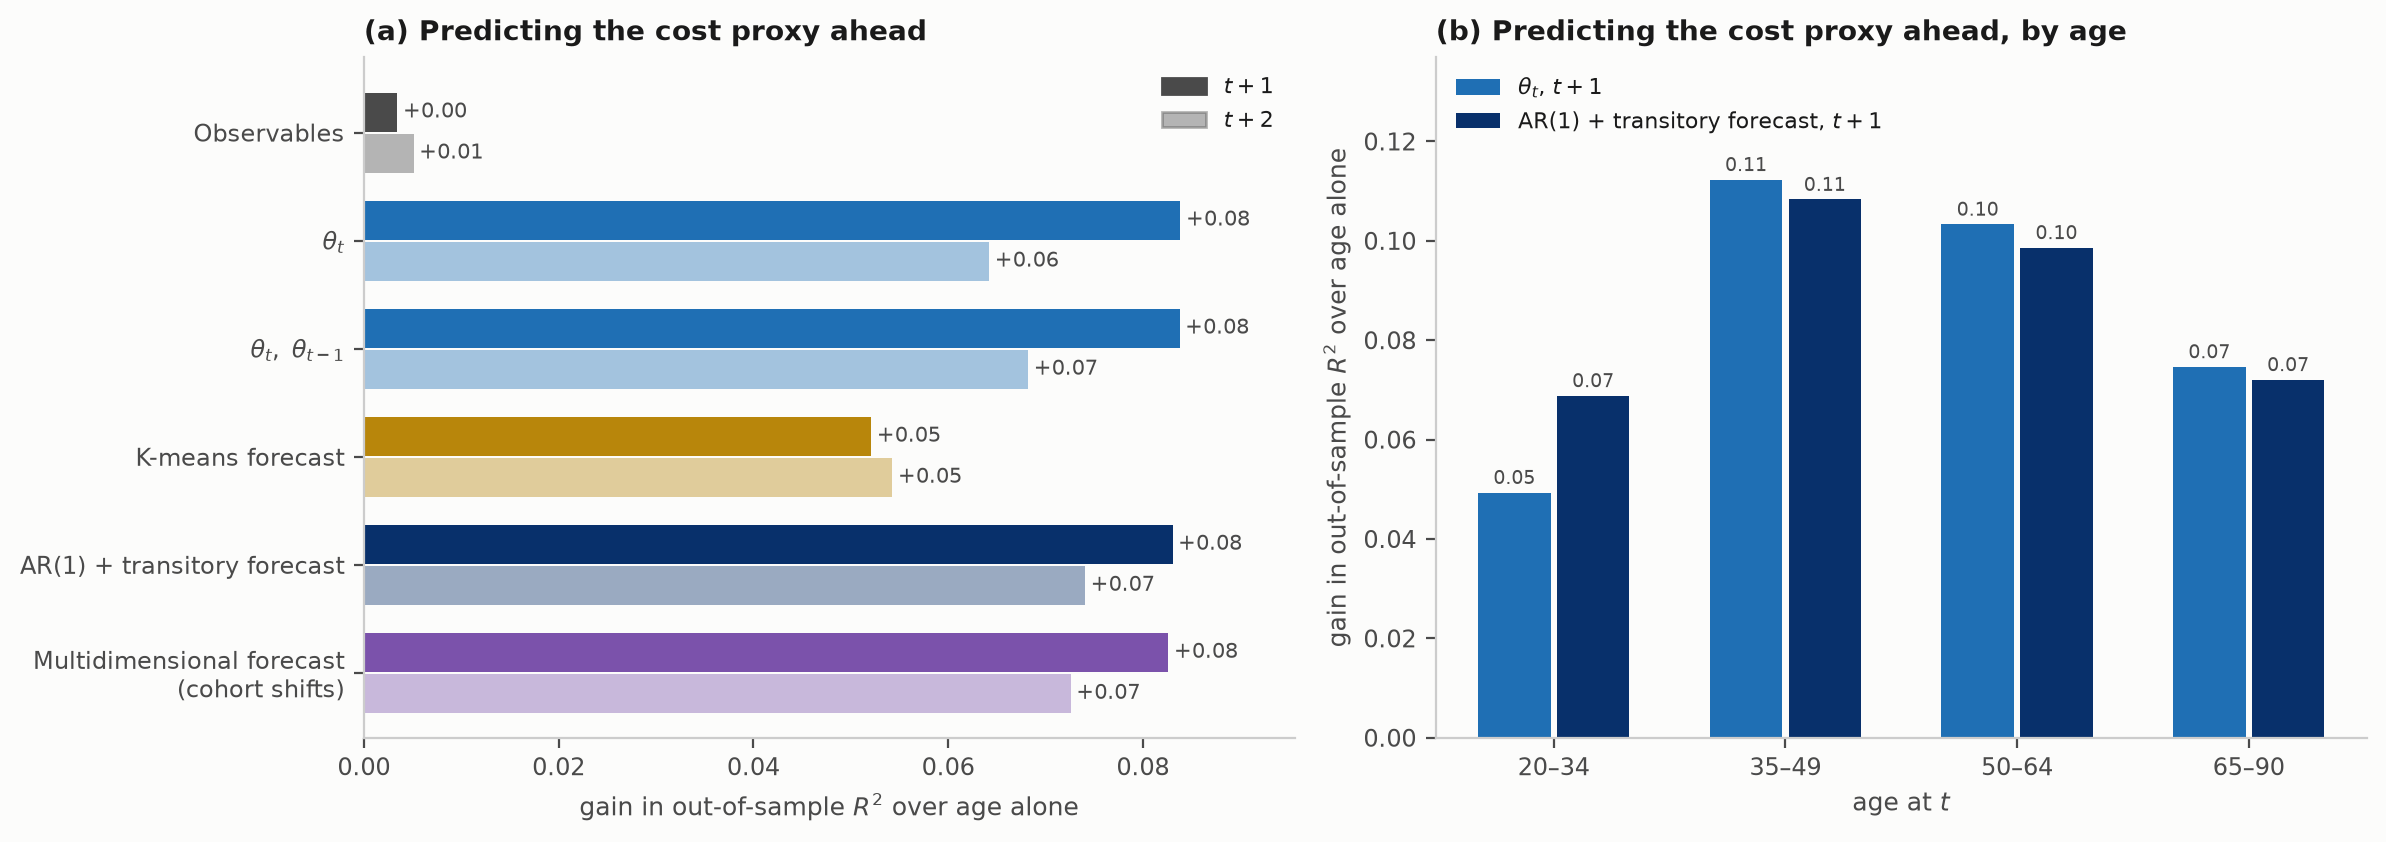
\includegraphics[width=\linewidth]{fig_prediction_cost.png}
	\caption{As Figure~\ref{fig:predsummary}(a), (c), predicting the cost proxy.}
	\label{fig:predcost}
\end{figure}
\begin{figure}[H]\centering
	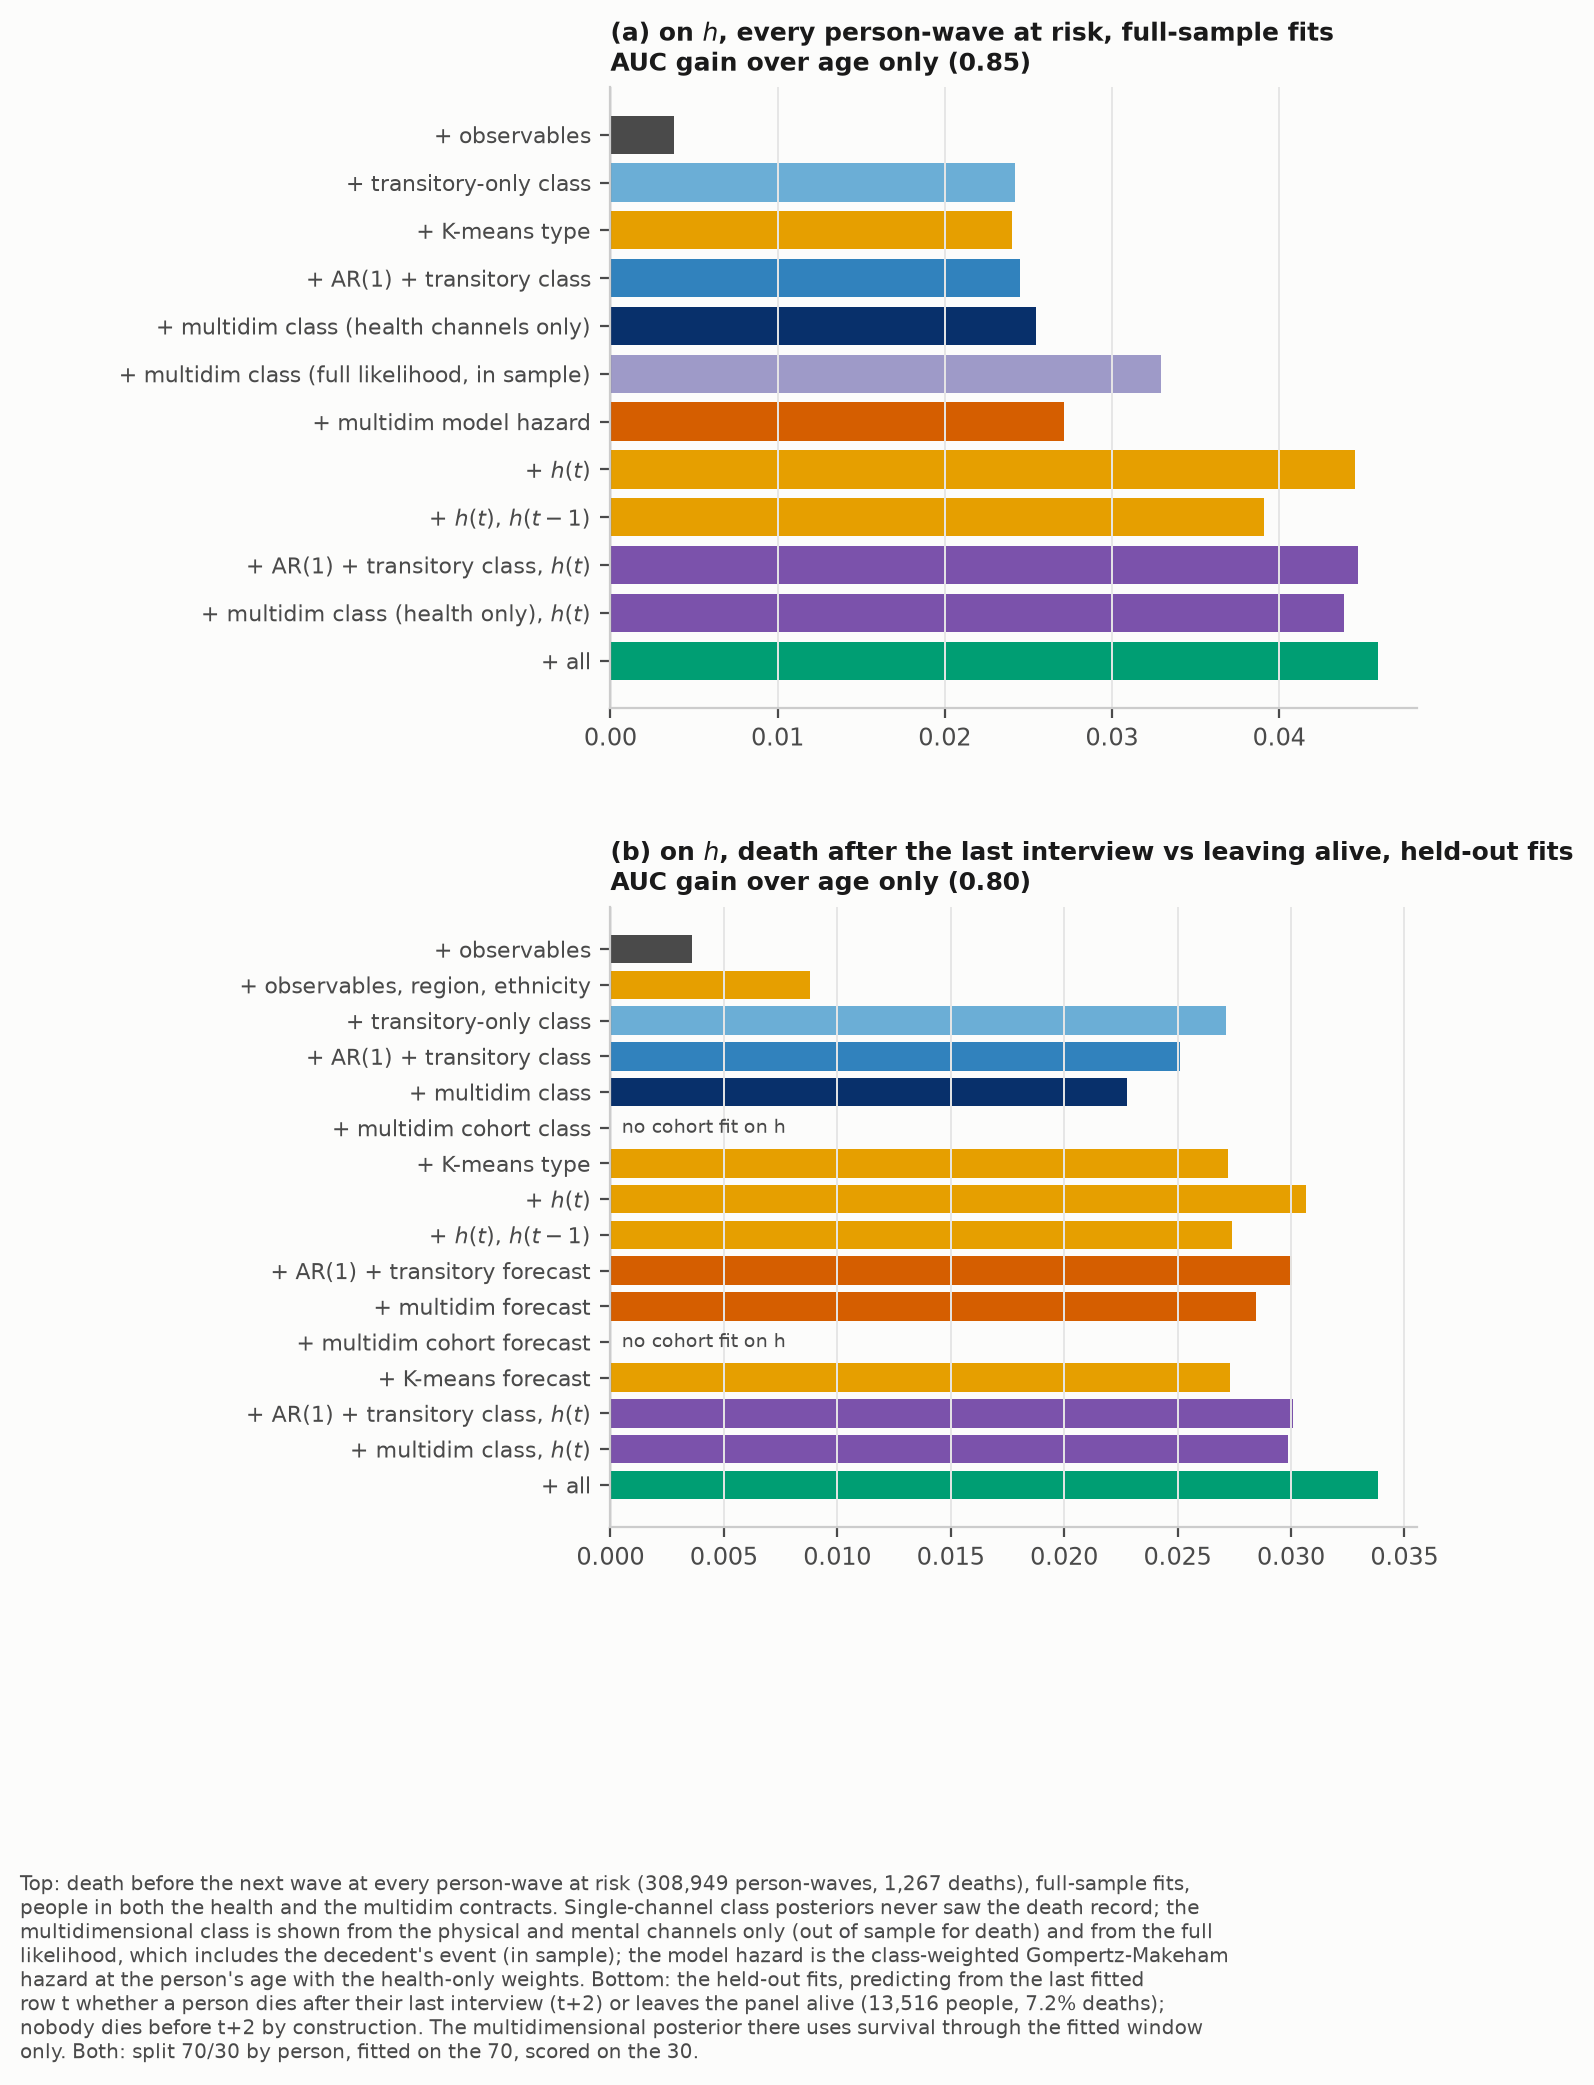
\includegraphics[width=0.62\linewidth]{fig_prediction_mortality_h.png}
	\caption{Predicting death on $h$.}
	\label{fig:predmort_h}
\end{figure}
\begin{figure}[H]\centering
	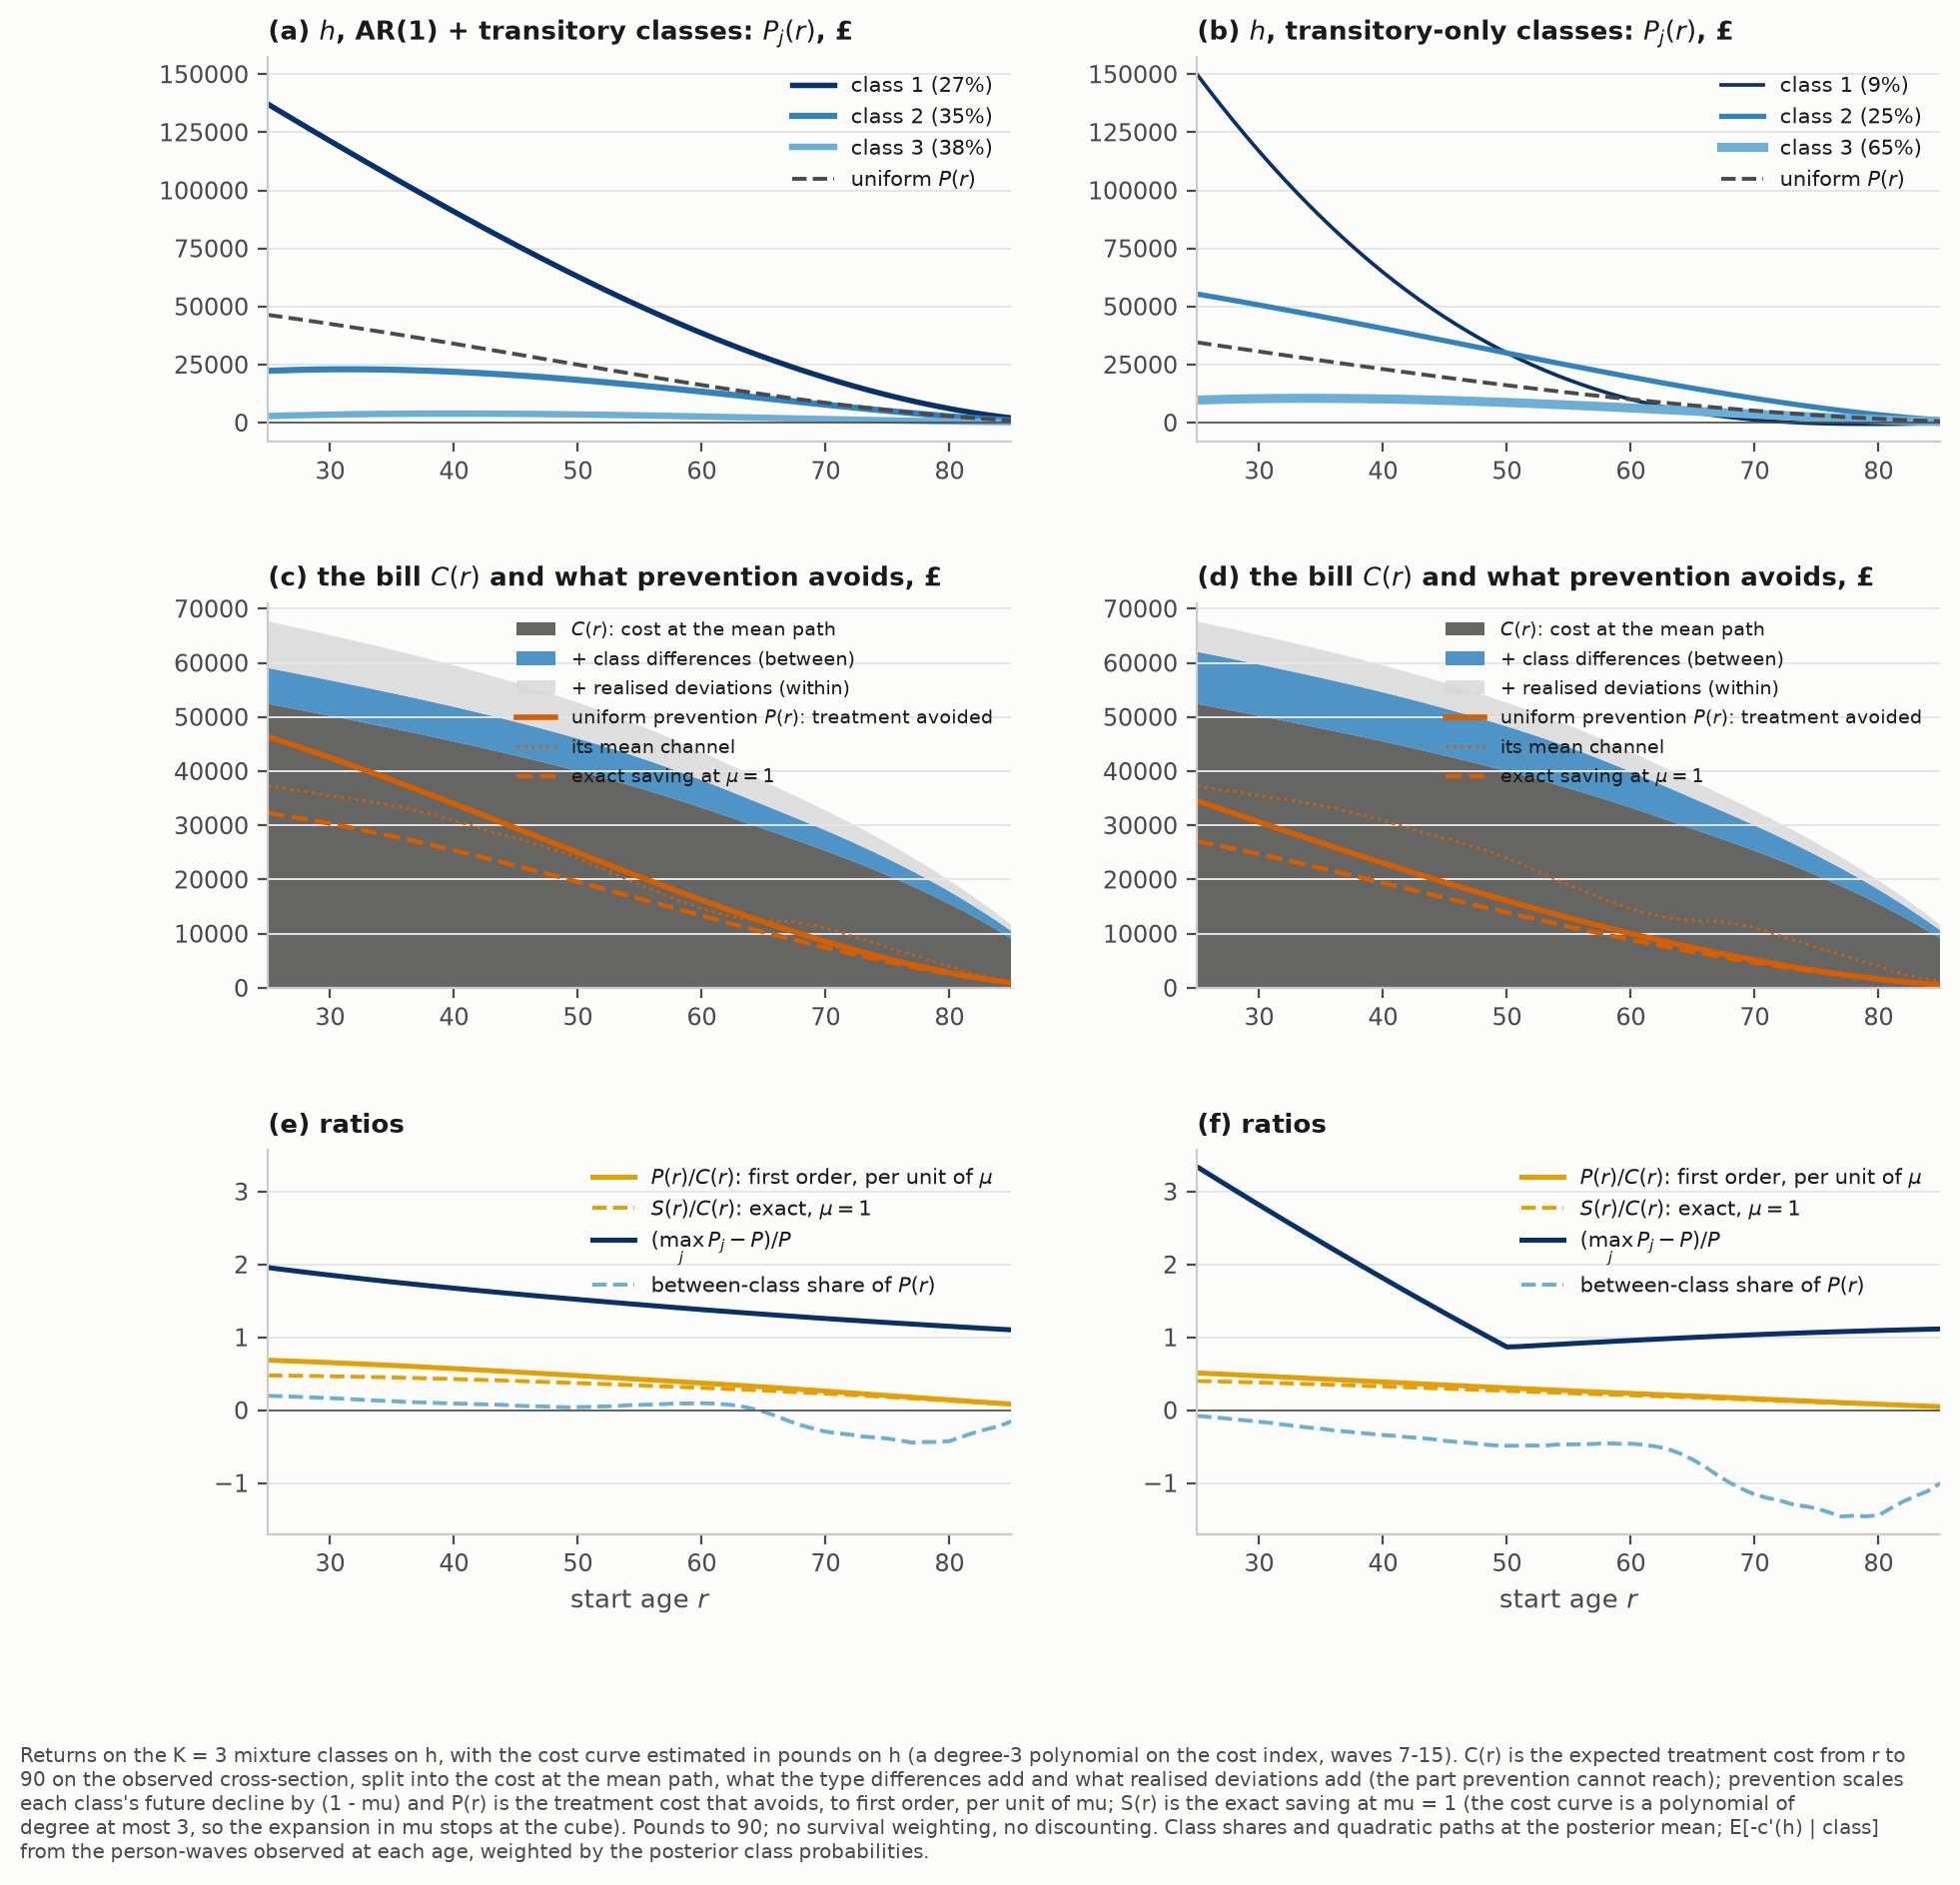
\includegraphics[width=\linewidth]{fig_returns_bayes_h.png}
	\caption{As Figure~\ref{fig:returnsbayes}, on $h$.}
	\label{fig:returnsbayes_h}
\end{figure}
\begin{figure}[H]\centering
	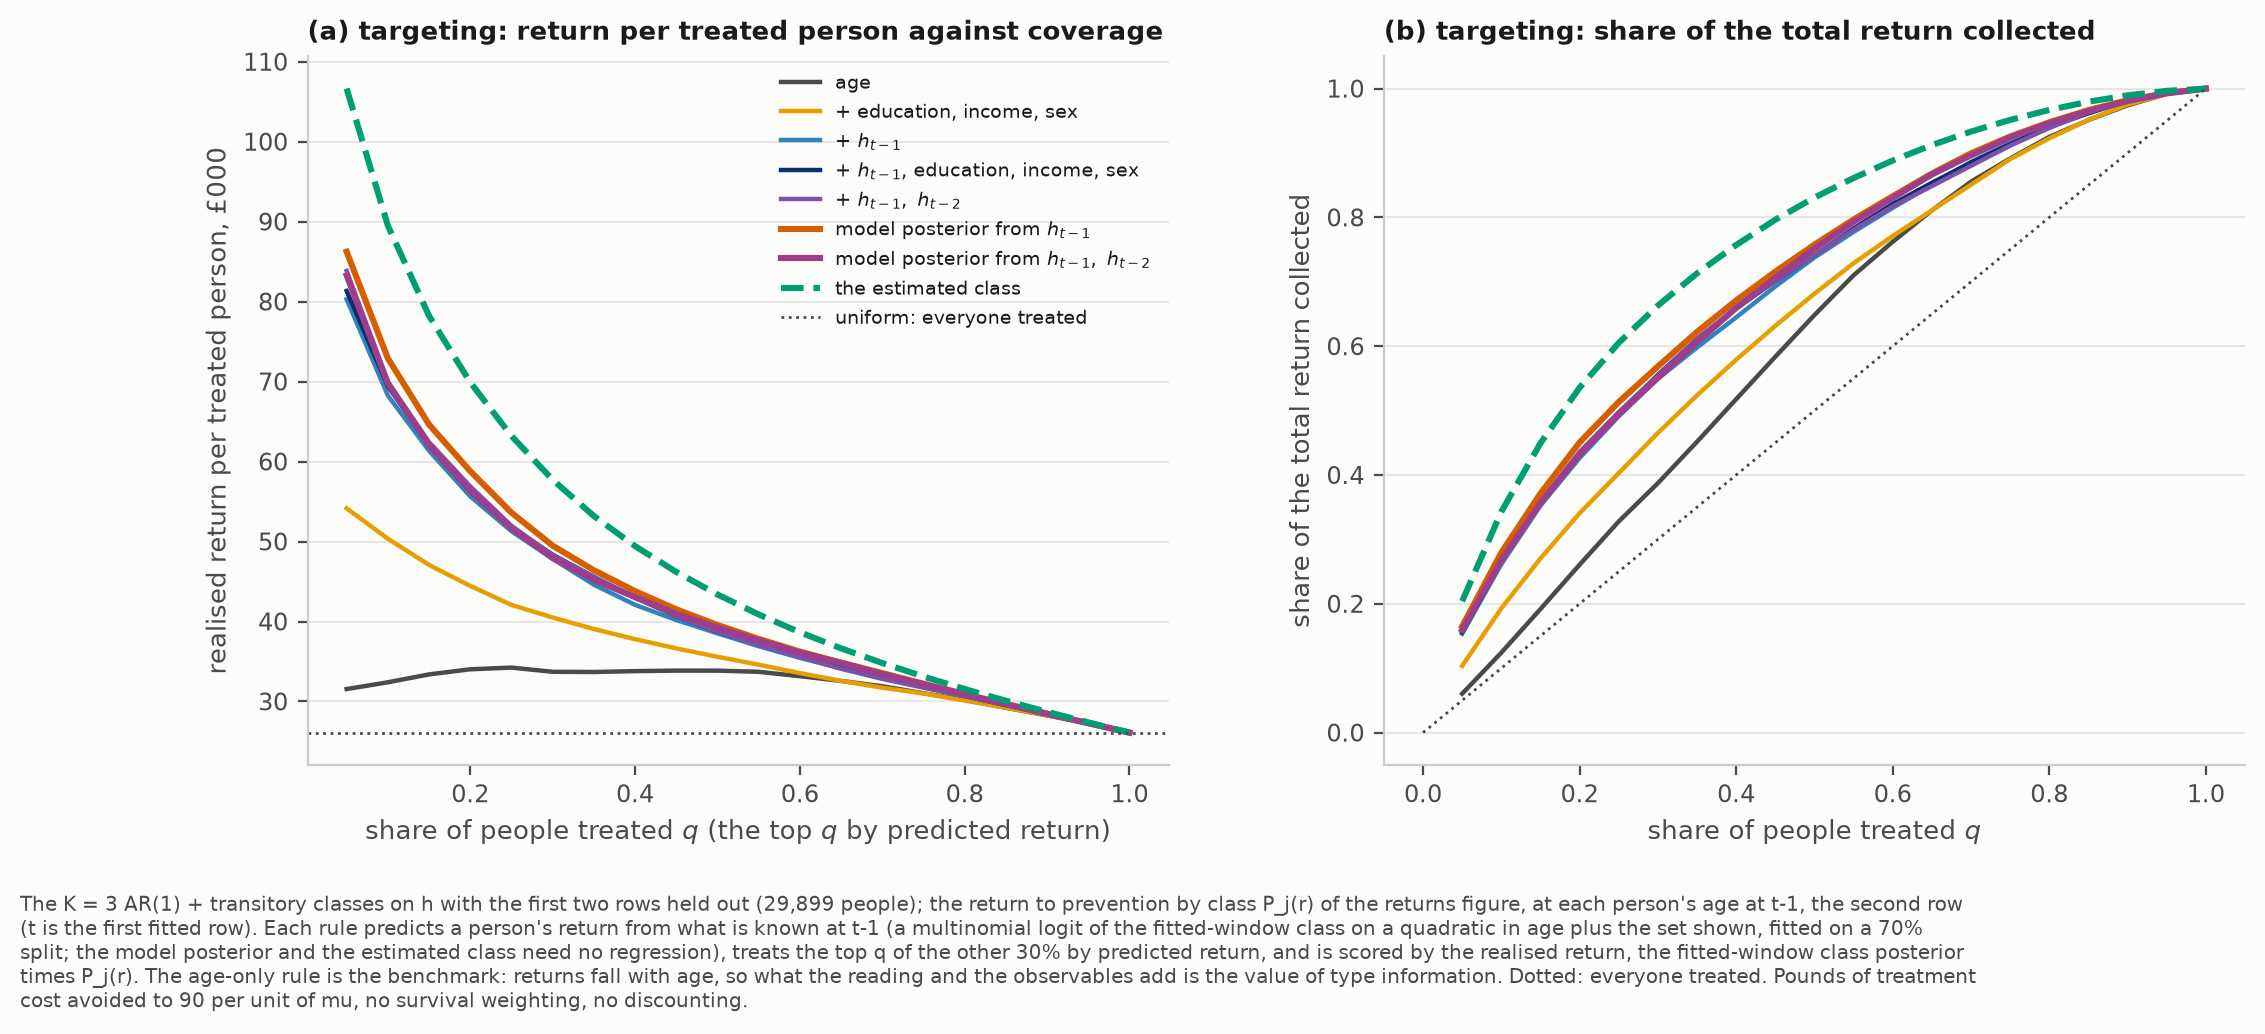
\includegraphics[width=\linewidth]{fig_targeting_first2_h.png}
	\caption{As Figure~\ref{fig:targeting}, on $h$.}
	\label{fig:targeting_h}
\end{figure}

\end{document}
